\documentclass[12pt,a4paper,twoside,openright]{report}
\let\openright=\cleardoublepage


%%% Choose a language %%%

\newif\ifEN
%\ENtrue   % uncomment this for english
\ENfalse   % uncomment this for czech

%%% Configuration of the title page %%%

\def\ThesisTitleStyle{mff} % MFF style
%\def\ThesisTitleStyle{cuni} % uncomment for old-style with cuni.cz logo
%\def\ThesisTitleStyle{natur} % uncomment for nature faculty logo

\def\UKFaculty{Faculty of Mathematics and Physics}
%\def\UKFaculty{Faculty of Science}

\def\UKName{Charles University in Prague} % this is not used in the "mff" style

% Thesis type names, as used in several places in the title
\def\ThesisTypeTitle{\ifEN BACHELOR THESIS \else BAKALÁŘSKÁ PRÁCE \fi}
%\def\ThesisTypeTitle{\ifEN MASTER THESIS \else DIPLOMOVÁ PRÁCE \fi}
%\def\ThesisTypeTitle{\ifEN RIGOROUS THESIS \else RIGORÓZNÍ PRÁCE \fi}
%\def\ThesisTypeTitle{\ifEN DOCTORAL THESIS \else DISERTAČNÍ PRÁCE \fi}
\def\ThesisGenitive{\ifEN bachelor \else bakalářské \fi}
%\def\ThesisGenitive{\ifEN master \else diplomové \fi}
%\def\ThesisGenitive{\ifEN rigorous \else rigorózní \fi}
%\def\ThesisGenitive{\ifEN doctoral \else disertační \fi}
\def\ThesisAccusative{\ifEN bachelor \else bakalářskou \fi}
%\def\ThesisAccusative{\ifEN master \else diplomovou \fi}
%\def\ThesisAccusative{\ifEN rigorous \else rigorózní \fi}
%\def\ThesisAccusative{\ifEN doctoral \else disertační \fi}



%%% Fill in your details %%%

% (Note: \xxx is a "ToDo label" which makes the unfilled visible. Remove it.)
\def\ThesisTitle{Analýza vazby mezi teplotou vzduchu ve standardní výšce a v hladině bylinného patra v závislosti na meteorologických podmínkách}
\def\ThesisAuthor{Vojtěch Klimeš}
\def\YearSubmitted{2023}

% department assigned to the thesis
\def\Department{Katedra fyziky atmosféry}
% Is it a department (katedra), or an institute (ústav)?
\def\DeptType{katedra}

\def\Supervisor{doc. Mgr. Michal Žák, Ph.D.}
\def\SupervisorsDepartment{Katedra fyziky atmosféry}

% Study programme and specialization
\def\StudyProgramme{Fyzika}
\def\StudyBranch{FP}

\def\Dedication{%
Dedication. \xxx{It is nice to say thanks to supervisors, friends, family, book authors and food providers.}
}

\def\AbstractEN{%
\xxx{Abstracts are an abstract form of art. Use the most precise, shortest sentences that state what problem the thesis addresses, how it is approached, pinpoint the exact result achieved, and describe the applications and significance of the results. Highlight anything novel that was discovered or improved by the thesis. Maximum length is 200 words, but try to fit into 120. Abstracts are often used for deciding if a reviewer will be suitable for the thesis; a well-written abstract thus increases the probability of getting a reviewer who will like the thesis.}
% ABSTRACT IS NOT A COPY OF YOUR THESIS ASSIGNMENT!
}

\def\AbstractCS{%
\xxx{You will need to submit both Czech and English abstract to the SIS, no matter what language you use in the thesis. If writing in English, translate the contents of \texttt{\textbackslash{}AbstractEN} into this field. In case you do not speak czech, your supervisor should be able to help you with the translation.}
}

% 3 to 5 keywords (recommended), each enclosed in curly braces.
% Keywords are useful for indexing and searching for the theses by topic.
\def\Keywords{%
\xxx{{key} {words}}
}

% If your abstracts are long and do not fit in the infopage, you can make the
% fonts a bit smaller by this setting. (Also, you should try to compress your abstract more.)
% Alternatively, consider increasing the size of the page by uncommenting the
% geometry modification in thesis.tex.
\def\InfoPageFont{}
%\def\InfoPageFont{\small}  %uncomment to decrease font size

\ifEN\relax\else
% If you are writing a czech thesis, you additionally need to fill in the
% english translation of the metadata here!
\def\ThesisTitleEN{Study of relationship between temperature measurement in standard level and herb layer according to meteorological conditions}
\def\DepartmentEN{Department of Atmospheric Physics}
\def\DeptTypeEN{Department}
\def\SupervisorsDepartmentEN{Department of Atmospheric Physics}
\def\StudyProgrammeEN{Physics}
\def\StudyBranchEN{FP}
\def\KeywordsEN{%
\xxx{{key} {words}}
}
\fi


\usepackage{siunitx}
\usepackage{subcaption}
\usepackage{amsmath}

\usepackage[a-2u]{pdfx}

\usepackage[czech,shorthands=off]{babel}
\usepackage[utf8]{inputenc}
\usepackage[T1]{fontenc}
% See https://en.wikipedia.org/wiki/Canons_of_page_construction before
% modifying the size of printable area. LaTeX defaults are great.
% If you feel it would help anything, you can enlarge the printable area a bit:
%\usepackage[textwidth=390pt,textheight=630pt]{geometry}
% The official recommendation expands the area quite a bit (looks pretty harsh):
%\usepackage[textwidth=145mm,textheight=247mm]{geometry}

%%% FONTS %%%
\usepackage{lmodern} % TeX "original" (this sets up the latin mono)

% Optionally choose an override for the main font for typesetting:
\usepackage[mono=false]{libertinus} % popular for comp-sci (ACM uses this)
%\usepackage{tgschola} % Schoolbook-like (gives a bit of historic feel)
%\usepackage[scale=0.96]{tgpagella} % Palladio-like (popular in formal logic).
% IBM Plex font suite is nice but requires us to fine-tune the sizes, also note
% that it does not directly support small caps (\textsc) and requires lualatex:
%\usepackage[usefilenames,RM={Scale=0.88},SS={Scale=0.88},SScon={Scale=0.88},TT={Scale=0.88},DefaultFeatures={Ligatures=Common}]{plex-otf}

% Optionally choose a custom sans-serif fonts (e.g. for figures and tables).
% Default sans-serif font is usually Latin Modern Sans. Some font packages
% (e.g. libertinus) replace that with a better matching sans-serif font.
%\usepackage{tgheros} % recommended and very readable (Helvetica-like)
%\usepackage{FiraSans} % looks great
% DO NOT typeset the main text in sans-serif font!
% The serifs make the text easily readable on the paper.

% IMPORTANT FONT NOTE: Some fonts require additional PDF/A conversion using
% the pdfa.sh script. These currently include only 'tgpagella'; but various
% other fonts from the texlive distribution need that too (mainly the Droid
% font family).


% some useful packages
\usepackage{microtype}
\usepackage{amsmath,amsfonts,amsthm,bm}
\usepackage{graphicx}
\usepackage{xcolor}
\usepackage{booktabs}
\usepackage{caption}
\usepackage{floatrow}

% load bibliography tools
%\usepackage[backend=bibtex,natbib,style=numeric,sorting=none]{biblatex}
% alternative with alphanumeric citations (more informative than numbers):
\usepackage[backend=biber,natbib,style=authoryear]{biblatex}
%
% alternatives that conform to iso690
% (iso690 is not formally required on MFF, but may help elsewhere):
%\usepackage[backend=bibtex,natbib,style=iso-numeric,sorting=none]{biblatex}
%\usepackage[backend=bibtex,natbib,style=iso-alphabetic]{biblatex}
%
% additional option choices:
%  - add `giveninits=true` to typeset "E. A. Poe" instead of full Edgar Allan
%  - `terseinits=true` additionaly shortens it to nature-like "Poe EA"
%  - add `maxnames=10` to limit (or loosen) the maximum number of authors in
%    bibliography entry before shortening to `et al.` (useful when referring to
%    book collections that may have hundreds of authors)
%  - for additional flexibility (e.g. multiple reference sections, etc.),
%    remove `backend=bibtex` and compile with `biber` instead of `bibtex` (see
%    Makefile)
%  - `sorting=none` causes the bibliography list to be ordered by the order of
%    citation as they appear in the text, which is usually the desired behavior
%    with numeric citations. Additionally you can use a style like
%    `numeric-comp` that compresses the long lists of citations such as
%    [1,2,3,4,5,6,7,8] to simpler [1--8]. This is especially useful if you plan
%    to add tremendous amounts of citations, as usual in life sciences and
%    bioinformatics.
%  - if you don't like the "In:" appearing in the bibliography, use the
%    extended style (`ext-numeric` or `ext-alphabetic`), and add option
%    `articlein=false`.
%
% possibly reverse the names of the authors with the default styles:
%\DeclareNameAlias{default}{family-given}

% load the file with bibliography entries
\addbibresource{refs.bib}
%\addbibresource{refs}

% remove this if you won't use fancy verbatim environments
\usepackage{fancyvrb}

% remove this if you won't typeset TikZ graphics
\usepackage{tikz}
\usetikzlibrary{arrows.meta}
\usetikzlibrary{positioning} %add libraries as needed (shapes, decorations, ...)
\usetikzlibrary{patterns}

% remove this if you won't typeset any pseudocode
\usepackage{algpseudocode}
\usepackage{algorithm}

% remove this if you won't list any source code
\usepackage{listings}


\hypersetup{unicode}
\hypersetup{breaklinks=true}

\usepackage[noabbrev]{cleveref}


% various forms of TODOs (you should remove this before submitting)
\usepackage[textsize=tiny, backgroundcolor=yellow!25, linecolor=black!25]{todonotes}
\newcommand{\xxx}[1]{\textcolor{red!}{#1}}

 % remove this before compiling the final version


% use this for typesetting a chapter without a number, e.g. intro and outro
\def\chapwithtoc#1{
\chapter*{#1}
\addcontentsline{toc}{chapter}{#1}
}

% If there is a line/figure overflowing into page margin, this will make the
% problem evident by drawing a thick black line at the overflowing spot. You
% should not disable this.
\overfullrule=3mm

% The maximum stretching of a space. Increasing this makes the text a bit more
% sloppy, but may prevent the overflows by moving words to next line.
\emergencystretch=1em

\ifEN
\theoremstyle{plain}
\newtheorem{thm}{Theorem}
\newtheorem{lemma}[thm]{Lemma}
\newtheorem{claim}[thm]{Claim}
\newtheorem{defn}{Definition}
\theoremstyle{remark}
\newtheorem*{cor}{Corollary}
\else
\theoremstyle{plain}
\newtheorem{thm}{Věta}
\newtheorem{lemma}{Lemma}
\newtheorem{claim}{Tvrzení}
\newtheorem{defn}{Definice}
\theoremstyle{remark}
\newtheorem*{cor}{Důsledek}
\fi

\newenvironment{myproof}{
  \par\medskip\noindent
  \textit{\ifEN Proof \else Důkaz \fi}.
}{
\newline
\rightline{$\qedsymbol$}
}

% real/natural numbers
\newcommand{\R}{\mathbb{R}}
\newcommand{\N}{\mathbb{N}}

% asymptotic complexity
\newcommand{\asy}[1]{\mathcal{O}(#1)}

% listings and default lstlisting config (remove if unused)
\DeclareNewFloatType{listing}{}
\floatsetup[listing]{style=ruled}

\DeclareCaptionStyle{thesis}{style=base,font={small,sf},labelfont=bf,labelsep=quad}
\captionsetup{style=thesis}
\captionsetup[algorithm]{style=thesis,singlelinecheck=off}
\captionsetup[listing]{style=thesis,singlelinecheck=off}

% Customization of algorithmic environment (comment style)
\renewcommand{\algorithmiccomment}[1]{\textcolor{black!25}{\dotfill\sffamily\itshape#1}}

% Uncomment for table captions on top. This is sometimes recommended by the
% style guide, and even required for some publication types.
%\floatsetup[table]{capposition=top}
%
% (Opinionated rant:) Captions on top are not "compatible" with the general
% guideline that the tables should be formatted to be quickly visually
% comprehensible and *beautiful* in general (like figures), and that the table
% "head" row (with column names) should alone communicate most of the content
% and interpretation of the table. If you just need to show a long boring list
% of numbers (because you have to), either put some effort into showing the
% data in an attractive figure-table, or move the data to an attachment and
% refer to it, so that the boredom does not impact the main text flow.
%
% You can make the top-captions look much less ugly by aligning the widths of
% the caption and the table, with setting `framefit=yes`, as shown below.  This
% additionally requires some extra markup in your {table} environments; see the
% comments in the example table in `ch2.tex` for details.
%\floatsetup[table]{capposition=top,framefit=yes}

\ifEN\floatname{listing}{Listing}
\else\floatname{listing}{Výpis kódu}\fi
\lstset{ % use this to define styling for any other language
  language=C++,
  tabsize=2,
  showstringspaces=false,
  basicstyle=\footnotesize\tt\color{black!75},
  identifierstyle=\bfseries\color{black},
  commentstyle=\color{green!50!black},
  stringstyle=\color{red!50!black},
  keywordstyle=\color{blue!75!black}}

% Czech versions of the used cleveref references (It's not as convenient as in
% English because of declension, cleveref is limited to sg/pl nominative. Use
% plain \ref to dodge that.)
\ifEN\relax\else
\crefname{chapter}{kapitola}{kapitoly}
\Crefname{chapter}{Kapitola}{Kapitoly}
\crefname{section}{sekce}{sekce}
\Crefname{section}{Sekce}{Sekce}
\crefname{subsection}{sekce}{sekce}
\Crefname{subsection}{Sekce}{Sekce}
\crefname{subsubsection}{sekce}{sekce}
\Crefname{subsubsection}{Sekce}{Sekce}
\crefname{figure}{obrázek}{obrázky}
\Crefname{figure}{Obrázek}{Obrázky}
\crefname{table}{tabulka}{tabulky}
\Crefname{table}{Tabulka}{Tabulky}
\crefname{listing}{výpis}{výpisy}
\Crefname{listing}{Výpis}{Výpisy}
\floatname{algorithm}{Algoritmus}
\crefname{algorithm}{algoritmus}{algoritmy}
\Crefname{algorithm}{Algoritmus}{Algoritmy}
\newcommand{\crefpairconjunction}{ a~}
\newcommand{\crefrangeconjunction}{ a~}
\fi
 % use this file for various custom definitions

\begin{document}
\overfullrule=0pt
% the layout is mandatory, edit only in dire circumstances

\pagestyle{empty}
\hypersetup{pageanchor=false}
\begin{center}

% top part of the layout, this actually differs between faculties

\def\ThesisTitleXmff{%
  \ifEN
    \centerline{\mbox{
\includegraphics[width=166mm]{img/logo-en.pdf}}}
  \else
    \centerline{\mbox{
\includegraphics[width=166mm]{img/logo-cs.pdf}}}
  \fi
  \vspace{-8mm}\vfill%
  {\bf\Large\ThesisTypeTitle}
  \vfill%
  {\LARGE\ThesisAuthor}\par
  \vspace{15mm}%
  {\LARGE\bfseries\ThesisTitle}
  \vfill%
  \Department}
\def\ThesisTitleCuniLogo#1{%
  {\large\UKName\par\medskip\par\UKFaculty }
  \vfill%
  {\bf\Large\ThesisTypeTitle}
  \vfill%
  \includegraphics[width=70mm]{#1}
  \vfill%
  {\LARGE\ThesisAuthor}\par
  \vspace{15mm}%
  {\LARGE\bfseries\ThesisTitle}
  \vfill%
  \Department\par}
\def\ThesisTitleXcuni{\ThesisTitleCuniLogo{img/uklogo.pdf}}
\def\ThesisTitleXnatur{\ThesisTitleCuniLogo{img/naturlogo.pdf}}

% choose the correct page and print it
\csname ThesisTitleX\ThesisTitleStyle\endcsname
% latex corner: X is the new @

\vfill

{
\centerline{\vbox{\halign{\hbox to 0.45\hsize{\hfil #}&\hskip 0.5em\parbox[t]{0.45\hsize}{\raggedright #}\cr
\ifEN Supervisor of the \ThesisGenitive thesis:
\else Vedoucí \ThesisGenitive práce: \fi
& \Supervisor \cr
\noalign{\vspace{2mm}}
\ifEN Study programme: \else Studijní program: \fi
& \StudyProgramme \cr
\noalign{\vspace{2mm}}
\ifEN Study branch: \else Studijní obor: \fi
& \StudyBranch \cr
}}}}

\vfill

\ifEN Prague \else Praha \fi
\YearSubmitted

\end{center}

\newpage

% remember to sign this!
\openright
\hypersetup{pageanchor=true}
\pagestyle{plain}
\pagenumbering{roman}
\vglue 0pt plus 1fill

\ifEN
\noindent
I declare that I carried out this \ThesisAccusative thesis independently, and only with the cited
sources, literature and other professional sources. It has not been used to obtain another
or the same degree.
\else
\noindent
Prohlašuji, že jsem tuto \ThesisAccusative práci vypracoval(a) samostatně a výhradně
s~použitím citovaných pramenů, literatury a dalších odborných zdrojů.
Tato práce nebyla využita k získání jiného nebo stejného titulu.
\fi

\ifEN
\medskip\noindent
I understand that my work relates to the rights and obligations under the Act No.~121/2000 Sb.,
the Copyright Act, as amended, in particular the fact that the Charles
University has the right to conclude a license agreement on the use of this
work as a school work pursuant to Section 60 subsection 1 of the Copyright~Act.
\else
\medskip\noindent
Beru na~vědomí, že se na moji práci vztahují práva a povinnosti vyplývající
ze zákona č. 121/2000 Sb., autorského zákona v~platném znění, zejména skutečnost,
že Univerzita Karlova má právo na~uzavření licenční smlouvy o~užití této
práce jako školního díla podle §60 odst. 1 autorského zákona.
\fi

\vspace{10mm}


\ifEN
\hbox{\hbox to 0.5\hsize{%
In \hbox to 6em{\dotfill} date \hbox to 6em{\dotfill}
\hss}\hbox to 0.5\hsize{\dotfill\quad}}
\smallskip
\hbox{\hbox to 0.5\hsize{}\hbox to 0.5\hsize{\hfil Author's signature\hfil}}
\else
\hbox{\hbox to 0.5\hsize{%
V \hbox to 6em{\dotfill} dne \hbox to 6em{\dotfill}
\hss}\hbox to 0.5\hsize{\dotfill\quad}}
\smallskip
\hbox{\hbox to 0.5\hsize{}\hbox to 0.5\hsize{\hfil Podpis autora\hfil}}
\fi

\vspace{20mm}
\newpage

% dedication

\openright

\noindent
\Dedication

\newpage

% mandatory information page

\openright

\vbox to 0.49\vsize{\InfoPageFont
\setlength\parindent{0mm}
\setlength\parskip{5mm}

\ifEN Title: \else Název práce: \fi
\ThesisTitle

\ifEN Author: \else Autor: \fi
\ThesisAuthor

\DeptType:
\Department

\ifEN Supervisor: \else Vedoucí bakalářské práce: \fi
\Supervisor, \SupervisorsDepartment

\ifEN Abstract: \AbstractEN \else Abstrakt: \AbstractCS \fi

\ifEN Keywords: \else Klíčová slova: \fi
\Keywords

\vss}\ifEN\relax\else\nobreak\vbox to 0.49\vsize{\InfoPageFont
\setlength\parindent{0mm}
\setlength\parskip{5mm}

Title:
\ThesisTitleEN

Author:
\ThesisAuthor

\DeptTypeEN:
\DepartmentEN

Supervisor:
\Supervisor, \SupervisorsDepartmentEN

Abstract:
\AbstractEN

Keywords:
\KeywordsEN

\vss}
\fi

\newpage

\openright
\pagestyle{plain}
\pagenumbering{arabic}
\setcounter{page}{1}


\tableofcontents

\chapwithtoc{Úvod}
Standartní meteorologické stanice záměrně neměří teplotu ve vegetaci. Typicky měří podmínky ve volné atmosféře ve standartizované výšce nad zemí. Data z těchto stanic, které jsou navzájem velmi dobře porovnatelná, určují globálně používaná klimatická data. Data mimo vegetaci neodrážejí podmínky, kterým jsou organismy v nich žijící vystaveny i přes to, že lesní porosty pokrývají až jednu třetinu pevninského povrchu.



Následky globálního oteplování dopadají na lesní organismy jinak kvůli porostu, který ovlivňuje mikroklima, kterému jsou vystaveny. Změny v porostu pak můžou významně ovlivnit podmínky pod ním. Dále ovšem může jít i o vliv topografie jako například sklon povrchu, který ovlivňuje mikroklima bylliného patra. 

Tato práce analyzuje rozdíl mezi teplotami v bylinném patře a ve výšce $\SI{2}{m}$ a rozdíl mezi naměřenými teplotami se snaží vysvětlit pomocí meteorologických proměnných jako vítr, oblačnost, vlhkost, srážky atp. 


!!!Odstavec o tom co je mikroklima, mezoklima, makroklima + tabulka viz Geiger: Climate near the ground



Introduction should answer the following questions, ideally in this order:
\begin{enumerate}
\item What is the nature of the problem the thesis is addressing?
\item What is the common approach for solving that problem now?
\item How this thesis approaches the problem?
\item What are the results? Did something improve?
\item What can the reader expect in the individual chapters of the thesis?
\end{enumerate}

Expected length of the introduction is between 1--4 pages. Longer introductions may require sub-sectioning with appropriate headings --- use \texttt{\textbackslash{}section*} to avoid numbering (with section names like `Motivation' and `Related work'), but try to avoid lengthy discussion of anything specific. Any ``real science'' (definitions, theorems, methods, data) should go into other chapters.
\todo{You may notice that this paragraph briefly shows different ``types'' of `quotes' in TeX, and the usage difference between a hyphen (-), en-dash (--) and em-dash (---).}

It is very advisable to skim through a book about scientific English writing before starting the thesis. I can recommend by.

\chapter{Analýza lesního mikroklimatu}
\label{chap:ch1}

V následující části \ref{chap:fyz} popíšeme fyzikální děje odehrávající se poblíž zemského povrchu z pohledu mikrometeorologie a mikroklimatologie. Od jednoduchých ilustračních příkladů se přesuneme k tomu jaký vliv má na mikroklima přítomnost vegetace \ref{chap:veg} a topografie \ref{chap:topo}. V závěřečné části této kapitoly \ref{chap:measure} bude popsáno jakým způsobem jsou meteorologické podmínky měřeny a nakonec v \ref{chap:sumavabavorskyles} se podíváme na klima typické pro Národní park Šumava a Bavorský les.

\section{Fyzikální pohled na děje při povrchu země} \label{chap:fyz}
Pro rovný a téměř homogenní povrch, který můžeme omezit zeshora a zespoda rovinnou, platí zjednodušenná rovnice. Tato rovnice vyjadřuje energetickou bilanci\cite{arya2001}

$$R_N = H + H_L + H_G + \Delta H_S,$$\label{eq:bilance}

kde $R_N$ je celková bilance záření, $H$ je tok tepla z nebo do atmosféry, $H_L$ je latentní teplo, $H_G$ je tok tepla ze země a $\Delta H_S$ je změna uchovaného tepla za jednotku času na jednotku plochy přes celou hloubku vrstvy. $\Delta H_S$ můžeme také interpretovat jako rozdíl mezi energií dodanou a odevzdanou z vrstvy která nás zajímá. Pak jestliže $\Delta H_S>0$ tak se vrstva ohřívá a pro $\Delta H_S<0$ tak se ochlazuje jelikož $H_{in}<H_{out}$. Většinou ovšem nemůžeme měřit přímo toky tepla, pokud nejde o jednoduchý příklad jako třeba na obrázku (+++), kde vidíme vývoj toku energie na povrchu vyschlého jezera. Přes den se povrch ohřívá díky dopadu slunečního záření $R_N>0$, část tepla uniká pod povrch tedy $H_G<0$ a část ohřívá atmosféru, která sama pouze velmi málo absorbuje záření $H<0$. Naopak v noci vyzařuje povrch dlouhovlnné záření a tím se ochlazuje tedy $R_N<0$, $H$ je téměř nulové a zahřátá půda zpětně ohřívá povrch tedy $H_G>0$. Po celou dobu jde o suchý povrch tedy $H_L=0$\cite{arya2001}.

\subsection{Vliv latentního tepla}
Latentní teplo, které značíme $H_L$, je veličina týkající se změny skupenství látek, v našem případě se týká vody. Formálně můžeme latentní teplo zavést jako $H_L = T\Delta s$, kde $T$ je teplota při které dochází ke změně skupenství a $\Delta s$ je rozdíl mezi molárními entropiemi obou fází\cite{callen1985}. Za standartního atmosférického tlaku $\SI{1013}{hPa}$ je měřné latentní teplo tání $H_{lT} = \SI{334}{kJ/kg}$ a latentní teplo vypařování $H_{lv} = \SI{2265}{kJ/kg}$. 

Výše jsme analyzovali situaci, kdy šlo o suchý povrch. Pro vlhký povrch se nám situace změní. Část tepla bude absorbována vodou a spotřebována na výpar. Můžeme ovšem mít i opačnou situaci, kdy dochází ke kondenzaci vodní páry a uvolňování latentního tepla. Analogicky můžeme uvažovat situaci v zimě, kdy je přítomná voda v pevném skupenství. V našem zjednodušenném příkladě je tedy přes den $H_L > 0$ a v noci $H_L < 0$. Schématicky to můžeme vidět na \ref{fig:schema}, kde velikost jednotlivých toků tepla je ovlivněna mnoha faktory\cite{arya2001}.

\begin{figure}
\centering
	\begin{tikzpicture}
  % Part a: Day
  \draw (-1,0) -- (4,0);
  \draw[pattern=north east lines] (-1,0) rectangle (4,-0.2);
	\draw[-{Stealth},thick] (1,3) -- (1,0) node[midway,left] {$R_N$};
  \draw[-{Stealth},thick] (2,0) -- (2,2) node[midway,right] {$H$};
  \draw[-{Stealth},thick] (3,0) -- (3,1) node[midway,right] {$H_L$};
  \draw[-{Stealth},thick] (0,-0.2) -- (0,-1) node[midway,left] {$H_G$};
  \node at (2,-2) {(a) Situace ve dne};
	\node at (-0.7,0.25) {\textit{Povrch země}};

  % Part b: Night
  \begin{scope}[xshift=6cm]
    \draw (-1,0) -- (4,0);
    \draw[pattern=north east lines] (-1,0) rectangle (4,-0.2);
    \draw[-{Stealth},thick] (1,0) -- (1,1.5) node[midway,left] {$R_N$};
    \draw[-{Stealth},thick] (2,0.75) -- (2,0) node[midway,right] {$H$};
    \draw[-{Stealth},thick] (3,0.5) -- (3,0) node[midway,right] {$H_L$};
    \draw[-{Stealth},thick] (0,-1) -- (0,-0.2) node[midway,left] {$H_G$};
    \node at (2,-2) {(b) Situace v noci};
  \end{scope}
	\end{tikzpicture}
\caption{Schéma toku tepla ve dne a v noci}
\label{fig:schema}
\end{figure}

Vliv vlhkosti a deště můžeme ilustrovat na takzvaném "oázovém efektu". V určitých situacích, se může hodnota $H_L$ stát v rovnici \eqref{eq:bilance} i dominantní složkou. Oázovým efektem nazýváme situaci, kdy vítr přináší suchý teplý vzduch přes chladnou a vlhkou oblast. Dochází k silnému výparu, který ochlazuje vlivem latentního tepla povrch země. Následně máme tok tepla $H$ negativní zatímco $H_L$ je větší a pozitivní. Může se stát, že i tok tepla v půdě $H_G$ změní znaménko, pokud povrch bude chladnější než půda. Vlhkost půdy má také vliv na albedo povrchu, způsobuje nárůst absorpce slunečního záření, tedy pokles albeda\cite{arya2001}.

\subsection{Vliv vegetace} \label{chap:veg}
\subsubsection{Albedo}
Albedo je koeficient udávající poměr mezi zářením a dopadajícím zářením, nabývá tedy hodnot v intervalu $\langle 0,1\rangle$, kde $0$ znamená, že povrch všechno záření pohlcuje, jde o ideálně černé těleso a $1$ znamená, že vše záření odráží. Už samotný typ povrchu má na albedo významným vliv, kde může dosahovat velmi různých hodnot ať už jde o písek, vodní plochu, odhalenou půdu, vlhkou půdu atd. Růst vegetace a jejího typu má ovšem také významným vliv na albedo s odlišnými hodnotami pro různé typy plodin a různé typy dřevin, ilustrační příklady jsou vidět v tabulce \ref{tab:albedo}. Hodnoty jsou závislé i na úhlu dopadu záření, vliv má i výška porostu nebo roční období\cite{arya2001,alma}.

(+++ tabulka)

\subsubsection{Vliv na tok tepla}
Do členů v rovnici \ref{eq:bilance} můžeme zahrnout i růst vegetace. V tu chvíli musíme počítat s významnou prostorovou závislostí všech toků tepla a záření. Následně jsou pro nás nejdůležitější hodnoty $R_N$, $H$ a $H_L$ nad vegetací, dále $\Delta H_S$ se skládá ze dvou částí a to změna tepla ve vzduchu, vegetaci atp. a změna energie biochemického původu skrze fotosyntézu a přesunu oxidu uhličitého. Latentní teplo se pak skládá z výparu a kondenzace vody a také z transpirace vody listy rostlin, mluvíme pak o evapotranspiraci\cite{arya2001}. 

Vliv na celkový tok energie má i výška porostu, například v lese může být nezanedbatelné uchované teplo v úrovni vegetace, které může způsobit, že prostředí reaguje pomalu na změny teplot a jiných veličin. Pro suchý porost může uchovaná energie dosahovat až $\SI{7}{\%}$ celkového toku energie skrz dopadající záření, situace se ovšem pro vlhký porost obrací a denní uchovaná energie může být záporná\cite{alma}. 

Podle \cite{alma} ovlivňuje teplotu hustota porostu. Jestliže měříme teplotu v řidším lese a sledujeme průběh teploty od země až po koruny stromů tak teplo snadněji prochází vegetací a tudíž budou při zemi podobné teploty jako ve výšce několika metrů nebo až v korunách stromů. Naopak pokud se nacházíme v hustějším lese tak bude teplota růst dříve v oblasti korun stromů a teplota při zemi může mít zpoždění několik hodin a nižší denní maximální hodnoty. V noci také může v řidším lese docházet k inverzi teplot zatímco v hustějším budou teploty podobné napříč porostem. 

Tok tepla v lese je ovlivněn i větrem. Jestliže fouká silný vítr, může docházet k rychlému přenosu energie mimo lesní porost\cite{alma}. 

\subsubsection{Vliv na rychlost větru}
Turbulence vzduchu je zodpovědná za přenos hmoty, tepla a hybnosti v oblasti blízko povrchu země. Bez turbulence by promíchávání probíhalo na molekulární úrovni a řádově menším měřítku. Na míru turbulence a promíchávání má vliv rychlost větru. Vegetace ovlivňuje nejen rychlost větru, ale také její profil. Například koruny stromů můžou rychlost větru výrazně snižovat zatímco, pokud blízko země nejsou menší stromy, keře nebo jiné překážky tak zde může být rychlost větru větší. To má pak vliv na teploty uvnitř porostu, které se mohou více podobat teplotám ve volném vzduchu. Tímto je zřejmé, že vliv na rychlost větru má i přítomnost listů a jejich absence v zimě \cite{alma}. 

\subsubsection{Vliv na vlhkost vzduchu}
V předchozím odstavci jsme zmínili transpiraci flóry, která slouží jako zdroj vodní páry. Ukázková situace v jehličnatém lese může vypadat tak že tlak vodní páry dosahuje dvou maxim a to při povrchu půdy z důvodu nižšího promíchávání vzduchu a výparu a v oblasti korun stromů kvůli listům. Druhé maximum bývá ovšem menší kvůli promíchávání se suchým vzduchem nad korunami stromů. Vzhledem k absolutním rozdíl tlaku vodních par v řádu jednotek milibarů tak změna relativní vlhkost napříč dnem a výškou je dána především teplotním zvrstvením \cite{alma}. 

\subsubsection{Vliv na rosu}
Stromy nejenže stíní povrch země před přímým slunečním zářením a ovlivňují vyzařování dlouhovlnného záření povrchem, ale také ovlivňují množství rosy. Při měření množství ranní rosy v různé vzdálenosti od kmene stromu bylo pozorováno, že množství rosy roste strmě do zhruba $\SI{2}{m}$ od kmene a dále pomaleji, doba po kterou zůstala rosa na zemi také se vzdáleností rostla a od vzdálenosti $\SI{4}{m}$ lehce klesala \cite{alma}.

\subsubsection{Vliv na déšť}
Listnaté, ale i jehličnaté stromy mají vliv na distribuci deště. Největší množství vody se objevuje na vnějším okraji ohraničeném korunou stromu. Stromy bez listů mají na prostorové rozložení srážek pouze minimální vliv. Pod jehličnaté stromy dopadá pouze $\SI{60}{\%}$ až $\SI{90}{\%}$ srážek a v oblasti okraje korun dopadá o $\SI{10}{\%}$ až $\SI{20}{\%}$ více srážek než v místě bez porostu. Lesní porost také při slabém dešti může úplně zabránit dopadu srážek na půdu. Množství vody, které takto dokážou stromy zachytit se může pohybovat od $\SI{1}{mm}$ do $\SI{3}{mm}$. Část vody je také ztracena výparem z povrchu listu, který je podpořen výraznějším promícháváním vzduchu v oblasti horní části korun stromů \cite{alma}.

\subsubsection{Vliv na sníh}
Množství sněhový srážek, které dopadnou na zem v lesním porostu záleží na několika faktorech. Jestliže jde o mokrý sníh pak snadno zůstává v korunách stromů, takto může být v korunách zachyceno až $\SI{10}{cm}$ sněhu. Suchý sníh má naopak snáze dopadne na zem. Množství zachyceného sněhu závisí také na typu vegatace, jestli jde o listnaté nebo jehličnaté stromy, případně jaký druh. Na jaře taje sníh v lese pomaleji a tedy jeho přítomnost je pro místní klima velmi důležité, jelikož funguje jako zásobník vody\cite{alma}.

\subsection{Vliv topografie} \label{chap:topo}
V odstavcích výše jsme vysvětlili jakým způsobem může ovlivnit vegetace podnebí. Ilustrovali jsme, že přítomnost flóry má významný vliv na celou řadu meteorologických proměnných, které následně ovlivňují teplotu v lese a život organismů. Nyní se budeme soustředit na vliv topografie na meteorologické proměnné. Pro standardizované meteorologické stanice je typické, že jsou postavené na posekané travnaté ploše, která není zastíněná a terén není nakloněn, v reálné krajině tohle ovšem neplatí.

\subsubsection{Vliv okraje lesa}
V oblasti okraje lesního porostu máme kontakt rozhraní dvou rozdílných vzduchových hmot. Geografická orientace má vliv na to jak dlouho svítí denní světlo na toto rozhraní. Množství dopadající energie může být pro okraj lesa orientovaný na jih i několikrát větší než pro okraj orientovaný na sever, to platí ovšem např. pro lesy v Evropě. Na rozhranní lesa a otevřené oblasti můžeme dokonce pozorovat vyšší teploty než uvnitř lesa a mimo něj, částečně to může být kvůli sníženému promíchávání vzduchu, větší absorpci slunečního záření, stínění dlouhovlnného záření a nižšímu výparu. Vliv na teplotu má i vítr. Jestliže fouká směrem do lesa, pak je tendence, aby teplota na okraji lesa byla podobná teplotě mimo les a naopak pro vítr směrem z lesa\cite{alma}.

\subsubsection{Vliv sklonu a orientace svahu}
Množství slunečního záření, které dopadne na povrch země závisí na mnoha faktorech. Musíme vzít v potaz zeměpisnou šířku, období v roce, denní čas, sklon svahu a orientaci svahu. Například pro svah s velkým sklonem na severní polokouli, který míří na sever se může stát, že v zimě nedostane po většinu dne žádné sluneční záření. Abychom dostali úplný obrázek musíme započítat i difúzní záření, které je primární složkou záření pokud je zataženo. Difúzní záření není do takové míry ovlivněné sklonem svahu\cite{alma}.

\subsubsection{Vliv údolí}
Nejen sklon a orientace svahu mají vliv na mikroklima. Jeden z dalších důležitých aspektů je jestli se místo, kterým se zabýváme nachází v údolí nebo zda-li jde o kopec. Topografie údolí má vliv hned několika způsoby. Studený vzduch je hustší a tudíž klesá do údolí, kde pak může vznikat kapsa studeného vzduchu, údolí je typické prostředí kde můžeme pozorovat inverzi vzduchu. Údolní topografie může způsobovat to že na dno dopadá menší množství slunečního záření, zároveň je ale dlouhovlnné záření částečně stíněno okraji údolí. Do údolí hůře proniká vítr a tudíž je zde snížená turbulence a tím i turbulencí předávané teplo. Pro velmi úzké a hluboké propadliny je půda významným zdrojem tepla. Všechny tyto faktory mají opačný vliv v případě kopců a obecně vyvýšených míst\cite{alma}. 

\subsubsection{Vliv topografie na vítr}
Vítr ovlivněný topografií terénu můžeme rozdělit na tři typy podle původu: kompenzační vítr, horský a údolní vítr a vítr spojený se sklonem svahu. V prvním případě jde o vítr způsobený nevyváženým ohřevem zemského povrchu. Na teplejším místě se izobary začnou zvedat a tím vzniká horizontální gradient tlaku mezi chladnou a teplejší oblastí. Vítr spojený se sklonem svahu má v noci tendenci jít z vyšších nadmořských poloh dolů a naopak během dne. Můžeme mít také situaci, kdy pozorujeme údolí, které se zároveň svažuje. Zde už je situace složitější.

Při svítání se začíná povrch údolí ohřívat. Vzduch u strany údolí stoupá nahoru, ale údolní vítr stále ještě fouká směrem dolů. Během dne údolní vítr oslabuje až dojde k obrácení jeho směru a údolím fouká nahoru. Později odpoledne vítr po svazích začne ustávat a fouká pouze údolní vítr do vyšších nadmořských výšek. Následně chladnější vzduch ze stran údolí začne klesat a v noci nakonec údolní vítr začne opět vát dolů stejně jako vítr po svazích údolí. Toto popisuje ukázkovou situaci za letního dne bez oblačnosti.

Vítr ovlivněný topografií může mít další podoby, které ovšem pro tuto práci nejsou zásadní. Můžeme zmínit mořský vánek mezi střídavě rychle se ohřívajícím pobřežím a relativně studeném moři ve dne a rychle chladnoucím pobřeží a relativně teplému moři v noci. Významný vítr spojený s horskou topografií pak dostává různé názvy jako fén v Alpách nebo mistrál ve Francii\cite{alma}.

\subsection{Rozdíl mezi teplotou při povrchu země a ve standardní výšce}
Teplotou ve standardní výšce se typicky myslí ve výšce $\SI{1}{m}-\SI{2}{m}$. Jestliže máme situaci, kdy na povrch svítí přímé sluneční záření, tak se můžou vyskytovat výrazné gradienty teplot a to až $\SI{10}{K/mm}-\SI{20}{K/mm}$. Tyto výrazné gradienty jsou ovliněné mnoha faktory jak například druh povrchu nebo jeho vlhkostí a dalšími jak bylo diskutováno výše. Dále kvůli nezanedbatelné velikosti teplotních senzorů je netriviální měřit teplotu povrchu\cite{arya2001}. 

\section{Analýza faktorů ovlivňující teplotu vzduchu v lesním porostu}
V předchozích odstavcích jsme diskutovali vliv vegetace a topografie na různé meteorologické proměnné. Tuto souvislost v následující části budeme diskutovat na konkrétní studii týkající se výzkumu ploch po střední Evropě.

\subsection{Vliv topografie a struktury krajiny na teplotu}
Při hledání vlivu topografie na rozdíl mezi teplotou v lesním porostu a na nejbližší meteorologické stanici ve střední Evropě se ve výzkumu \cite{ZellwegerFlorian2019Sdou} hledala souvislost pomocí následujících prediktorů.

\begin{itemize}
	\item Plocha pokrytá lesním porostem v okruhu $\SI{250}{m}$ vyjádřená v procentech. Zde nebyla nalezena spojitost s rozdílem teplot.
	\item Vzdálenost k okraji lesa byla nevýznamným prediktorem. 
	\item Vzdálenost k nejbližšímu pobřeží a výška nad mořem byly nejsilnějšími prediktory, zároveň jde ovšem o silně korelované veličiny. Slabšími prediktory pak bylo stočení svahu k severu/jihu, sklon svahu a hodnota udávající zda-li jde spíše o údolí nebo vyvýšenné místo.
\end{itemize}

Tyto výsledky ovšem nejsou nutně konzistentní mezi různými studiemi. Například podle \cite{GreiserCaroline2018Mmmi} je plocha pokrytá lesním porostem důležitou hodnotou a může vést ke zvýšení minimální denní teploty až o $\SI{3}{\degree C}$ nebo vzdálenost k okraji lesa je středně silný prediktor.

\subsection{Vliv porostu na teplotu}
Druhou skupinou prediktorů kterou se \cite{ZellwegerFlorian2019Sdou} zabýval byly proměnné týkající se porostu v blízkém okolí čidla.

\begin{itemize}
	\item Zápoj má nelineární a záporný vliv na maximální teploty. Pod hodnotou $\SI{89}{\%}$ dochází k prudkému nárůstu vlivu vegetace.
	\item Otevřenost porostu vyjádřená jako část viditelné oblohy a plocha koruny stromů také má záporný nelineární vztah k maximální teplotě.
	\item Procento plochy pokryté dřevinami nad určitý průměr je pouze slabým prediktorem. 
	\item Výška stromu na kterém bylo čidlo upevněno naopak souvisí s rozdílem maximální teplot kladně, ale opět zde vztah není příliš silný.
	\item Schopnost porostu vytvářet stín podle typu dřeviny je středním prediktorem rozdílu maximálních teplot.
\end{itemize}

\subsection{Vliv meteorologických podmínek na teplotu}
Jak bylo zmíněno v předchozí části tak na rozdíl mezi teplotou mimo porost ať už lesní nebo jiný má vliv mnoho faktorů od topografických po konkrétní typ porostu. Tyto faktory se dají vyjádřit mnoha různými prediktory jejichž vliv můžeme sledovat. Aktuální stav počasí je ovšem další faktorem, který ovlivňuje naměřené teploty. Tím může být oblačnost, vlhkost, sněhová pokrývka, srážky, rychlost větru a roční doba.

V praktické části práce se budeme zabývat tím jaký vliv mají tyto proměnné na rozdíl mezi teplotou naměřenou v lesním porostu v národním parku Šumava ve výšce $\SI{2}{m}$ a při povrchu, tedy $\SI{0}{cm}$ a $\SI{15}{cm}$. Použitá čidla kromě teploty ještě půdní vlhkost, ostatní proměnné jsou z nejbližší meteorologické stanice.

\section{Popis měření meteorologický veličin} \label{chap:measure}
\subsection{Měření na meteorologických stanicích}
Teplota vzduchu by podle Světové meteorologické organizace (WMO) měla být měřena ve výšce $\SI{1.25}{m}$ až $\SI{2}{m}$\cite{wmoGuidance2021}. V České republice Český hydrometeorologický ústav provozuje celou řadu meteorologických stanic různého charakteru, ať už jde o SYNOP stanice nebo jiné +++. Měření probíhá standardizovaným způsobem, stanice by měla být na trávníku nikoliv například na asfaltu a měření probíhají v pravidelných intervalech. Pro synoptické stanice je to například v takzvaných hlavních termínech ($00$, $06$, $12$ a $18$ UTC) a případně vedlejších ($03$, $09$, $15$, $21$ hodin UTC). Podobně jsou na stanicích měřeny i další veličiny jako například, vlhkost, výška sněhu, část zatažené oblohy, tlak a další. 

\subsection{Měření v terénu pomocí čidel}
Pomocí meteorologických stanic není možné získat detailní informace o teplotě a dalších veličinách na malých prostorových škálách. Standartní meteorologické stanice nemůžou změřit teplotu například v lesním porostu. Data použitá v této práci jsou měřená pomocí TMS (Temperature-Moisture-Sensor) logger, kromě čidel jako například Thermochron iButtons, je možné využít radiometrie (+++) a z vyzářeného záření z povrchu pomocí Stefan-Boltzmannova zákona spočítat teplotu povrchu. Poslední metoda má ovšem své omezení pokud chceme znát teplotu v lesním porostu. 

\subsubsection{TMS4 a T1 logger} \label{chap:loggers}
Čidlo TMS4 logger používané pro sběr dat vědci a vědkyněmi z Botanického ústavu Akademie věd České republiky je konstruováno tak, aby měřilo podmínky, které prožívá malá bylinna. Je tedy vysoké $\SI{15}{cm}$ nad povrch země a sahá do hloubky $\SI{14}{cm}$. Je opatřeno třemi teplotními senzory ve výškách $\SI{15}{cm},\ \SI{0}{cm},\ \SI{-8}{cm}$. Až do hloubky $\SI{14}{cm}$ je měřena volumetrická půdní vlhkost. Vršek data loggeru je opatřen optickým stíněním z bílého plastu chránící horní senzor před přímým slunečním zářením a stejně tak je odstíněn i senzor při povrchu země. 

Teplotní senzor měří s přesností $\SI{\pm 0.5}{\degree C}$ a funguje na intervalu $\SI{-55}{\degree C}$ až $\SI{125}{\degree C}$. Měření volumetrické půdní vlhkostí je založené na time-domain-transmission (TDT), kdy jsou skrze obvod vysílány elektromagnetické pulzy a množství detekovaných pulzů je přímo úměrné vlhkosti. 

Při srovnání TMS4 loggeru se standartní meteorologickou stanicí typu METEOS 5 byla pozorována větší variabilita u teplot v $\SI{15}{cm}$ než ve $\SI{2}{m}$. TMS4 loggeru byl instalován na krátkém posekaném trávníku, tři metry od stanice a rozdíl teplot při hodinovém měření se pohyboval od $\SI{+8.45}{\degree C}$ do $\SI{-6.05}{\degree C}$. Průměrné denní teploty naměřené z TMS4 loggeru byly systematicky nižší, průměrný rozdíl ovšem pouze $\SI{-0.58}{\degree C}$, v zimě jsou tyto rozdíly větší a to $\SI{-2.02}{\degree C}$ až $\SI{0.6}{\degree C}$. Opačný trend pak můžeme pozorovat, pokud není teplotní senzor v $\SI{15}{cm}$ odstíněn plastovým krytem. V létě byly teploty nižší až o $\SI{5.08}{\degree C}$, ale v zimě byly podobné. Teploty z půdních senzorů jak TMS4 loggeru tak stanice METEOS 5 se lišily velmi málo, rozdíl mezi naměřenými teplotami byl tedy zřejmě způsoben primárně polohou senzorů a použitým stíněním než jejich typem. Rozdíly mězi naměřenými teplotami nad zemí byly ještě výraznější pro proměnné, které jsou často používány v ekologických studiích jako například kvantily extrémních teplot\cite{WildJan2019Caer}. 

Data měřená při povrchu země jsou na některých místech doplněna stejnými teplotními senzory ve výšce $\SI{2}{m}$ upevněnými na kmenu stromu a také opatřena plastovým stínítkem.

\section{Národní park Šumava} \label{chap:sumavabavorskyles}
Čidla TMS logger z kterých pocházejí data použitá v této práci jsou v oblasti Národní parku Šumava. Národní park Šumava vyhlášený v roce 1991 má rozlohu $\SI{680}{km^2}$. Jeho výška se pohybuje od $\SI{600}{m.\ n.\ m.}$ do $\SI{1378}{m.\ n.\ m.}$. Nejvyšší bod je vrchol Plechý. Více než $\SI{80}{\%}$ územi pokrývá les. Šumava je v rámci Evropy jedno z nejstarších pohoří, tvořené je metamorfovanými horninami jako ruly a svory a žulovými masivy. Typické pro toto území jsou horské smrčiny, rašeliniště, karová jezera a pralesní porosty.


\chapter{Analýza dat} \label{chap:analysis}
V první části druhé kapitoly se zaměříme na popis struktury použitých dat. V druhé části analyzujeme autokorelační a prostorovou složku dat, a hledat vhodný model pro vysvětlení rozdílů naměřených teplot.

\section{Využitá data z ČHMÚ}
Pro hledání souvislosti mezi meteorologickými podmínkami a rozdílem teplot na čidlech poblíž země jsme využili data z meteorologických stanic Churáňov, Borová Lada, Kvilda, Horská Kvilda a Javoří pila. Nejvíce informací jsme získali ze synoptické stanice Churáňov. Z dostupných dat jsme pro další analýzu využili data o aktuální teplotě ve výšce $\SI{2}{m}$, rychlosti větru, výšce sněhové pokrývky, hodinových srážek a oblačnosti. Z ostatních stanic jsme měli k dispozici hodinová data o výšce sněhové pokrývky a pro Borovou Ladu informace o úhrnu srážek.

Analýzu provádíme pro období od 12.10.2019 do 21.5.2021 i když v případě některých čidel kvůli výpadkům měření bude zpracovávaný interval kratší (viz kapitola \ref{chap:data_buav}).

Na obrázku \ref{fig:chmuukazka} můžeme vidět ukázku dat z meteorologické stanice Churáňov. Maximální teplota ($\SI{27}{\degree C}$) za období 12.10.2019 až 20.5.2021 byla naměřena 21.8.2020 a minimální ($\SI{-16.1}{\degree C}$) byla naměřena 11.2.2021 a 13.2.2021. Největší sněhová pokrývka byla $\SI{48}{cm}$ 31.1.2021.

\begin{figure}
	\centering
	\begin{subfigure}{0.45\textwidth}
  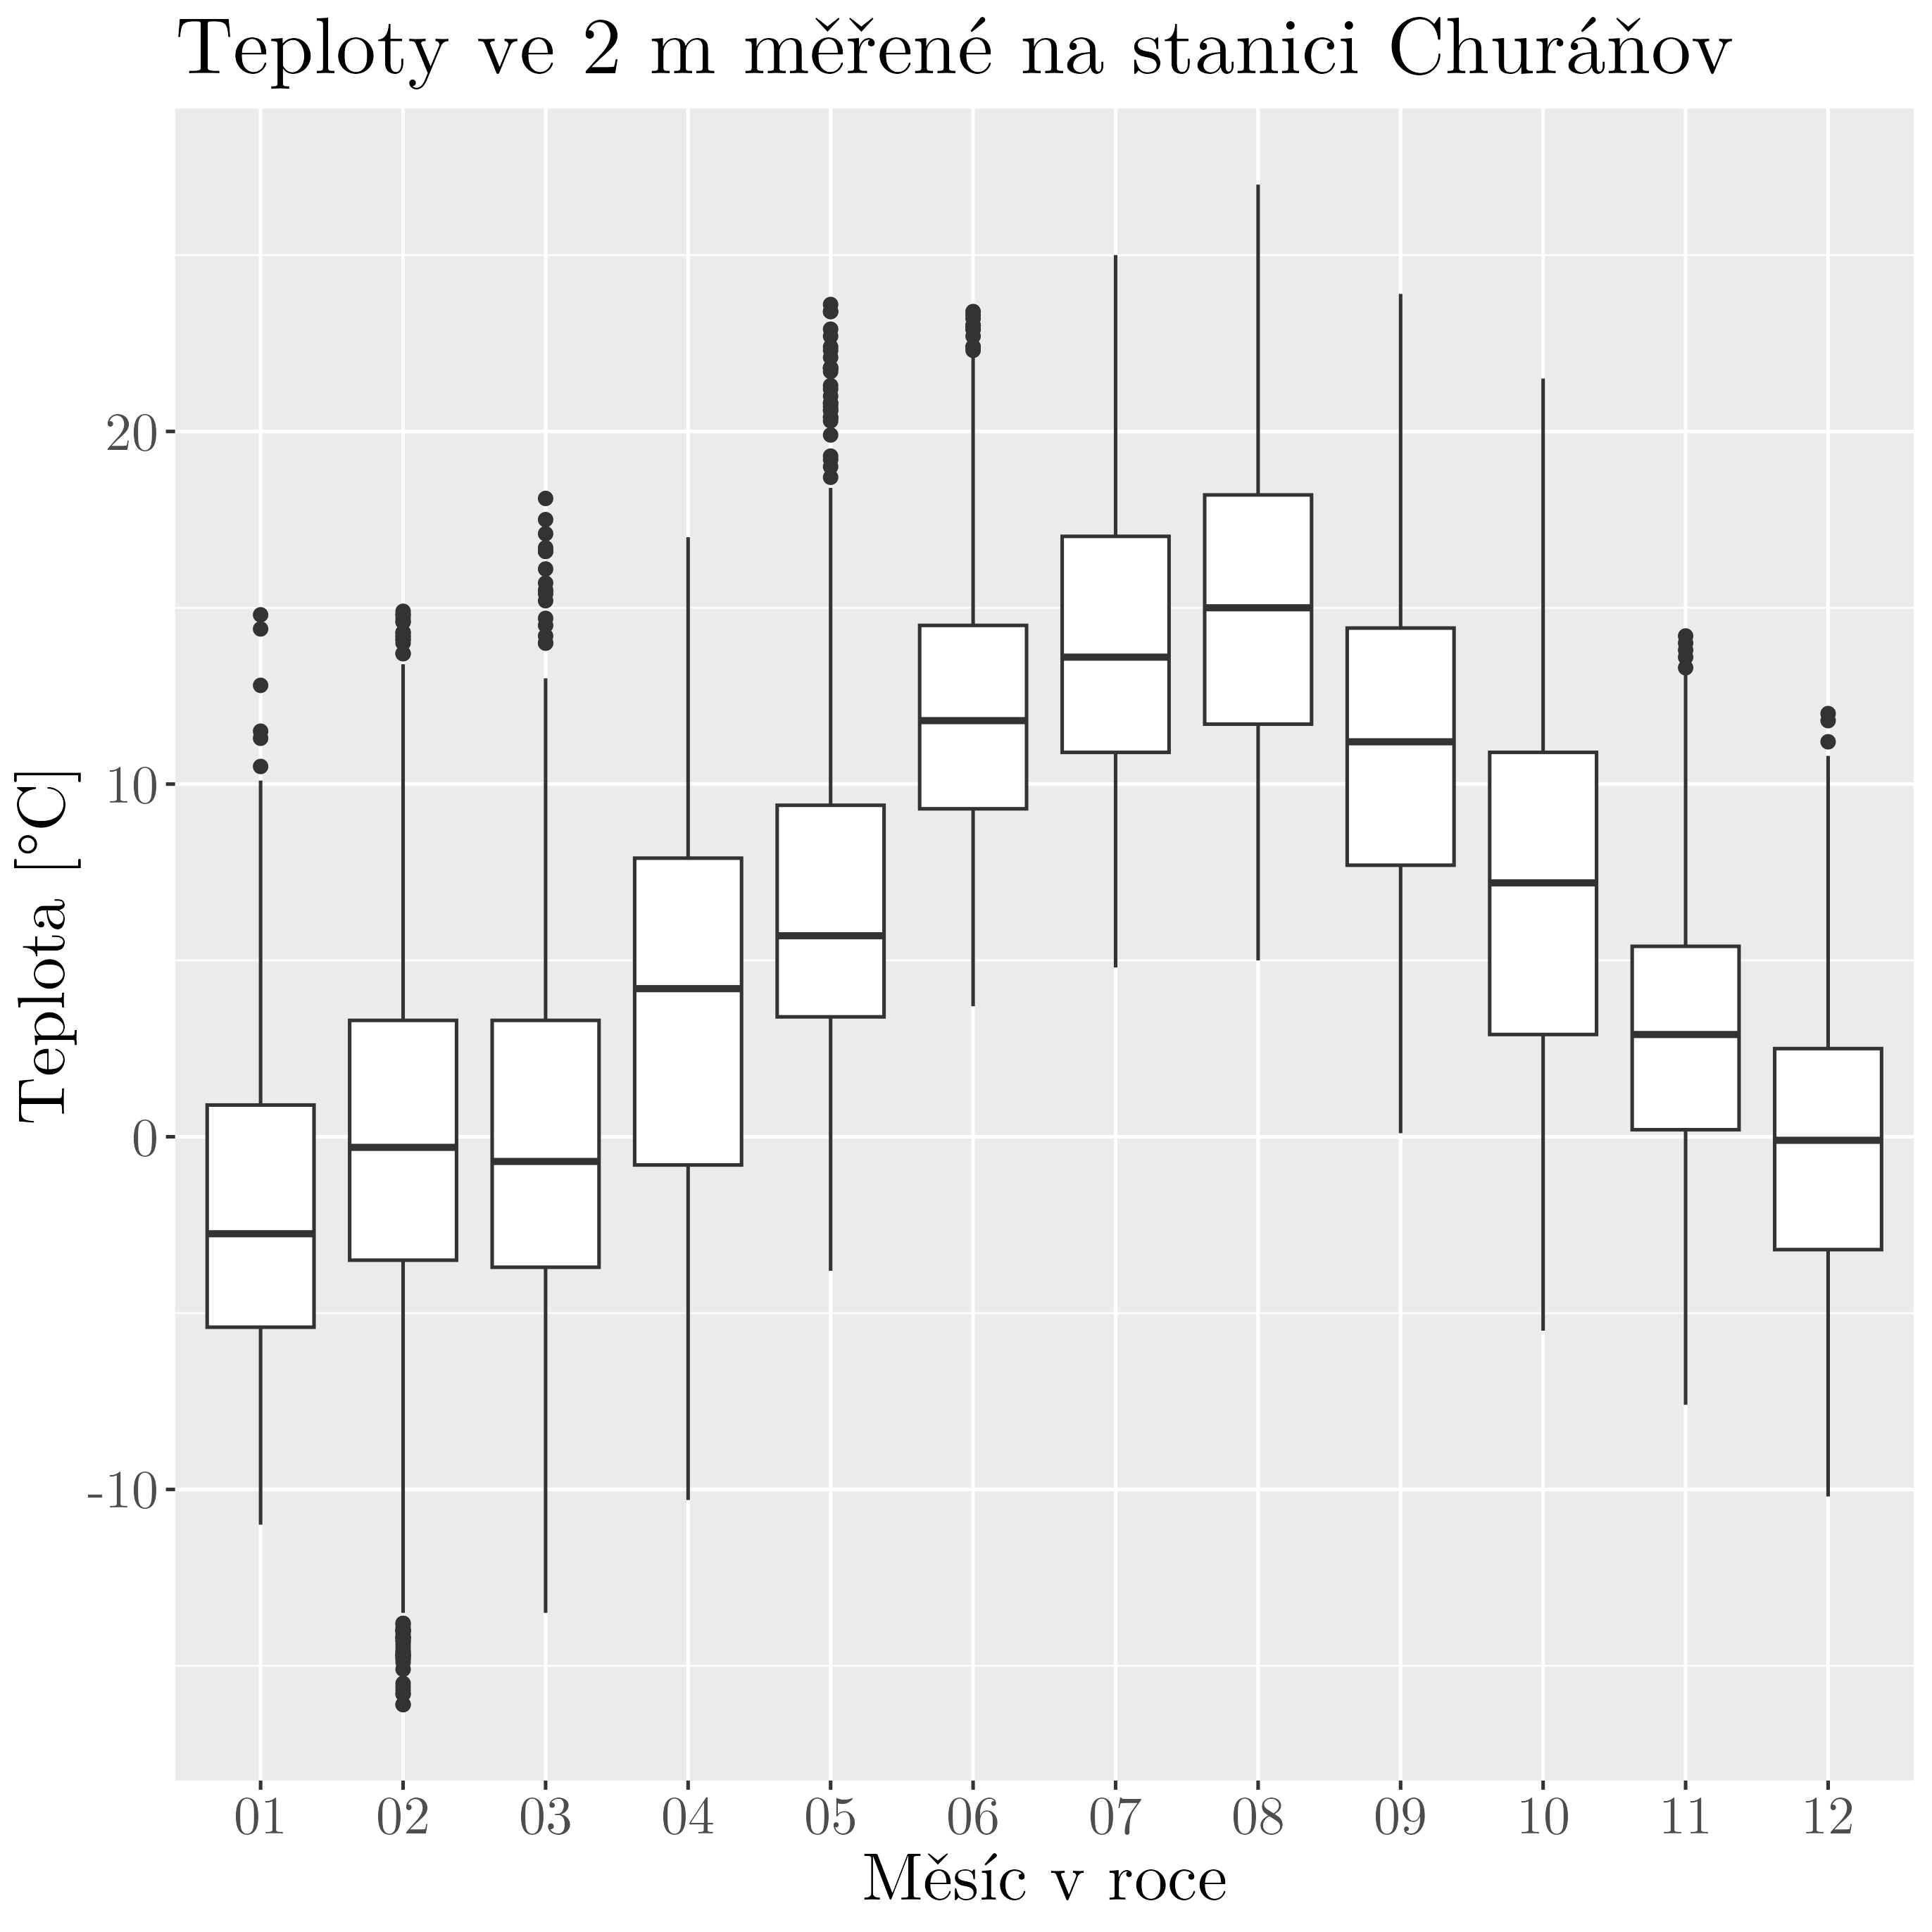
\includegraphics[width=\textwidth]{img/synop_temperature.png}
		\caption{Okamžité denní teploty rozdělené podle měsíců v roce.}
		\label{fig:synop_temperature}
	\end{subfigure}
	\hfill
	\begin{subfigure}{0.45\textwidth}
  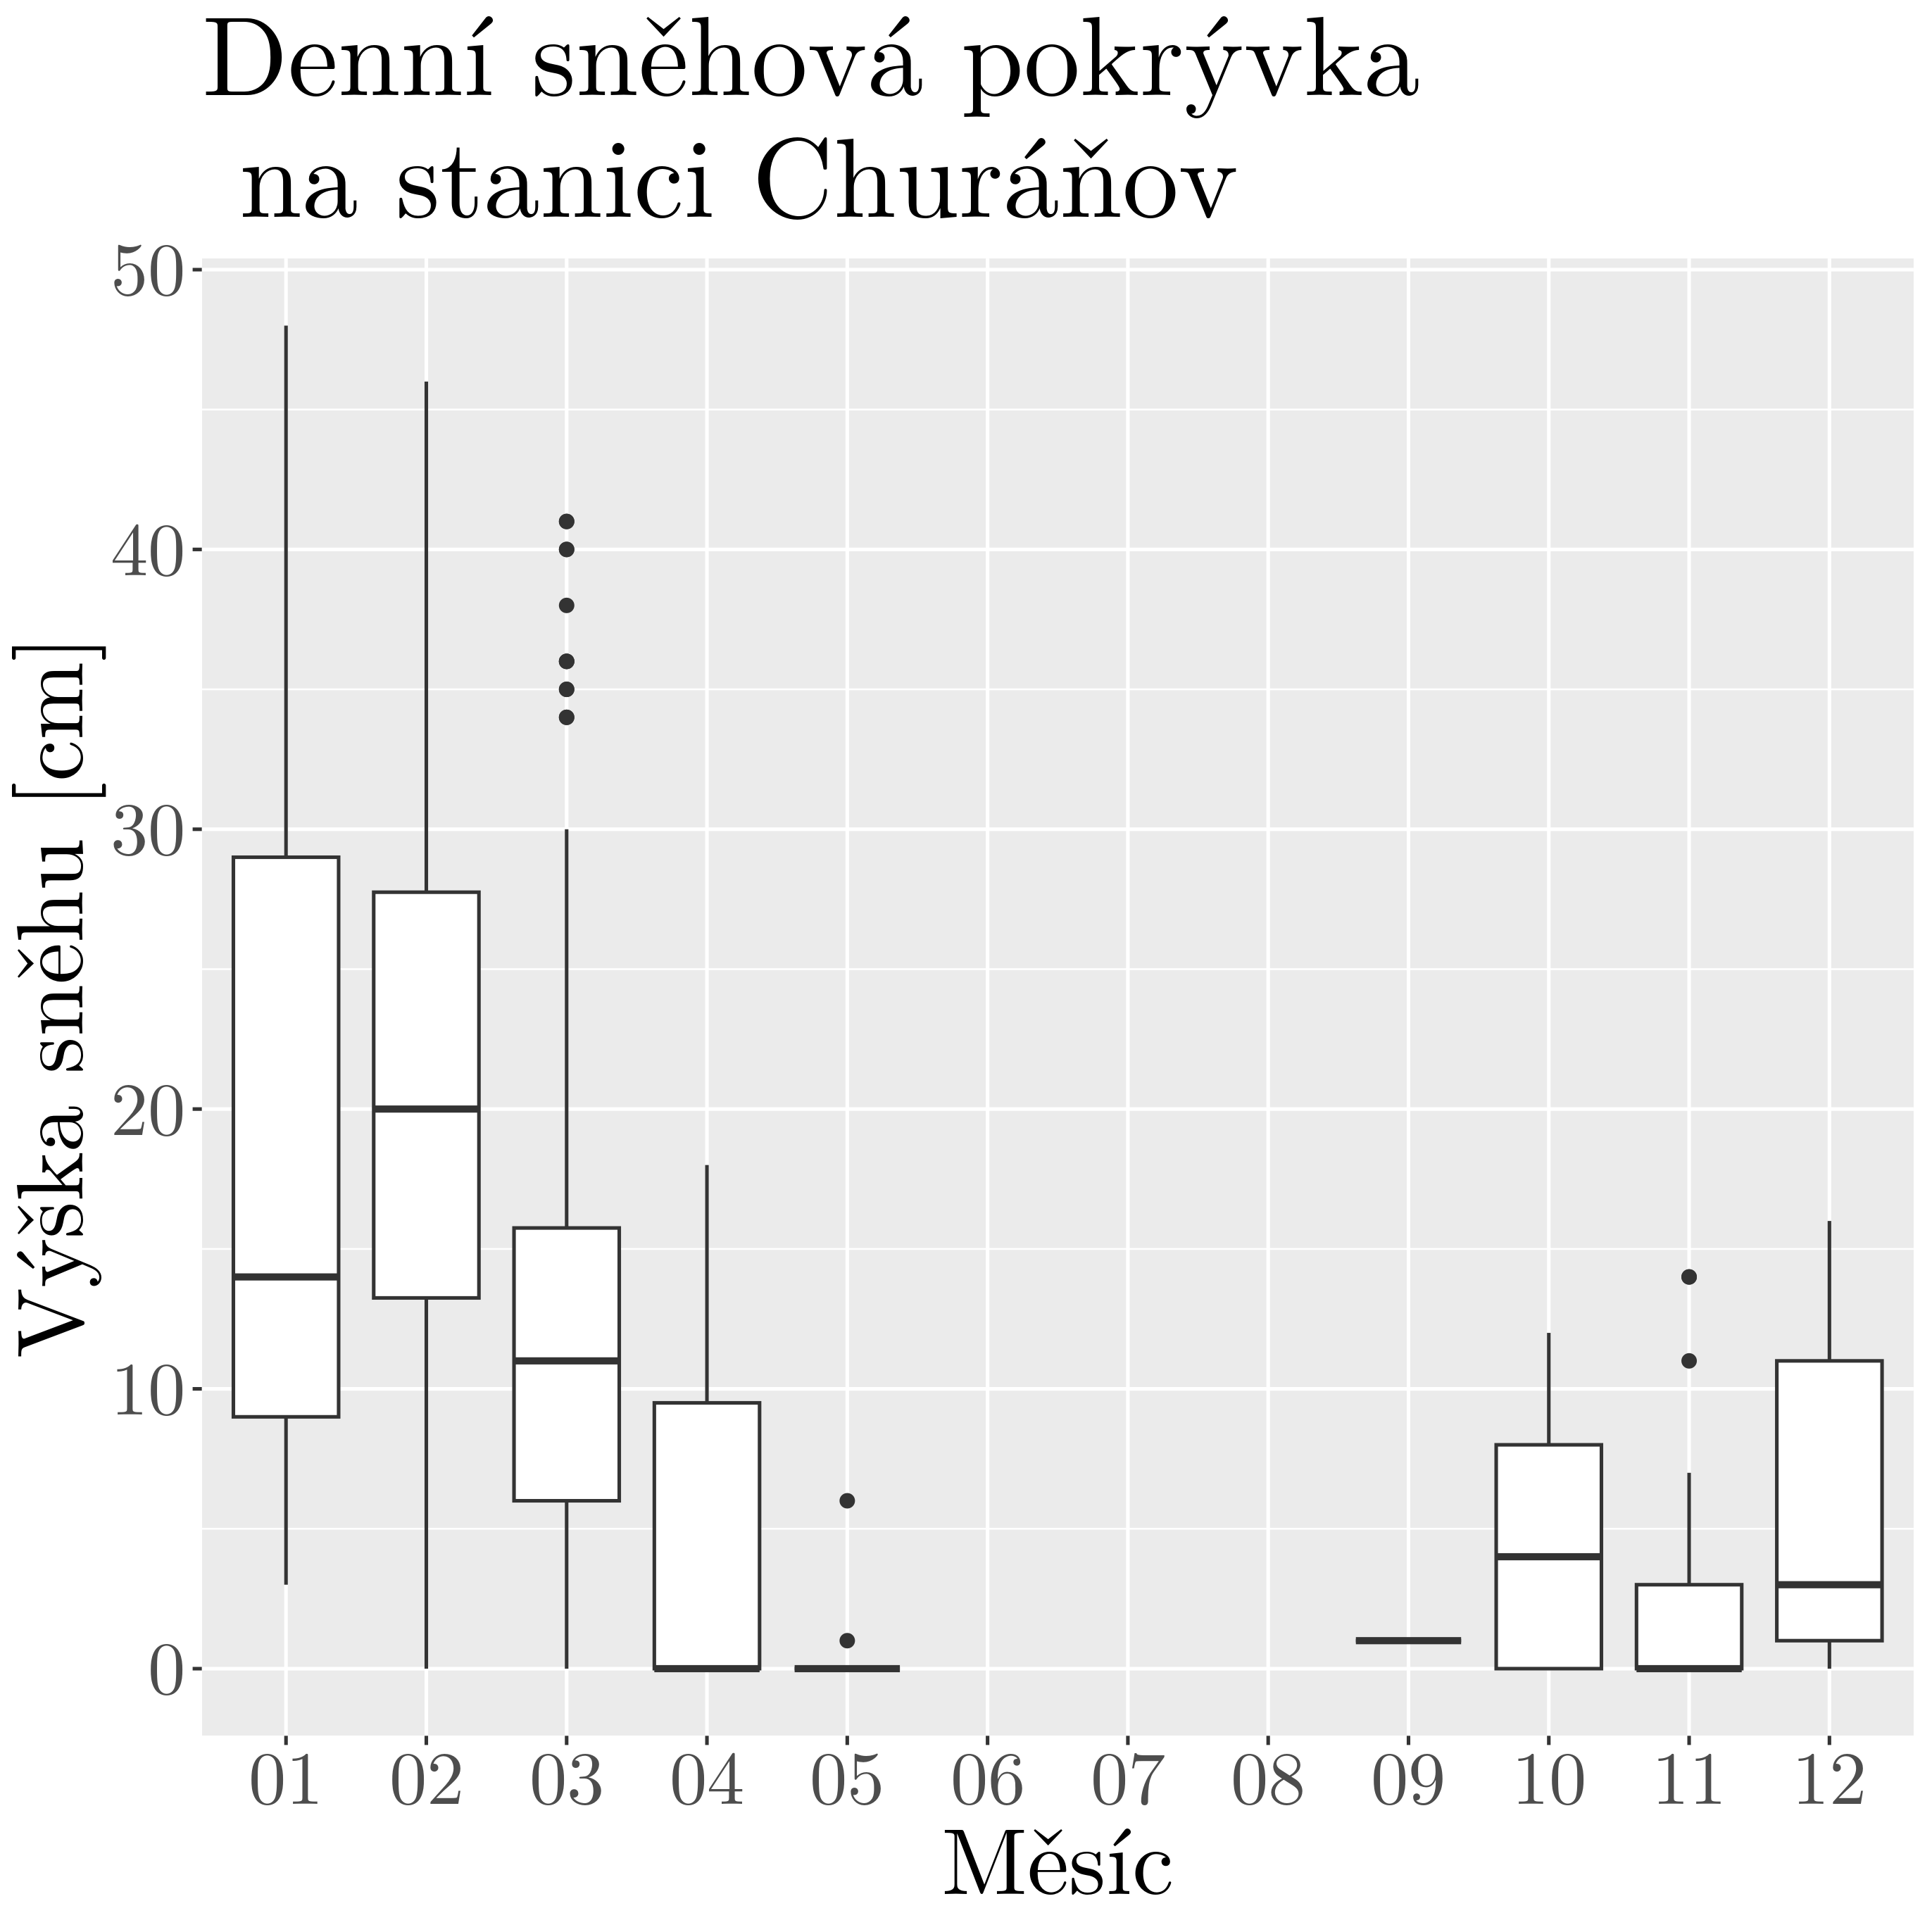
\includegraphics[width=\textwidth]{img/ch2/hist_snow_synop_bymonth.png}
		\caption{Denní sněhová pokrývka.}
		\label{fig:synop_snowcm}
	\end{subfigure}
	\hfill
	\begin{subfigure}{0.45\textwidth}
  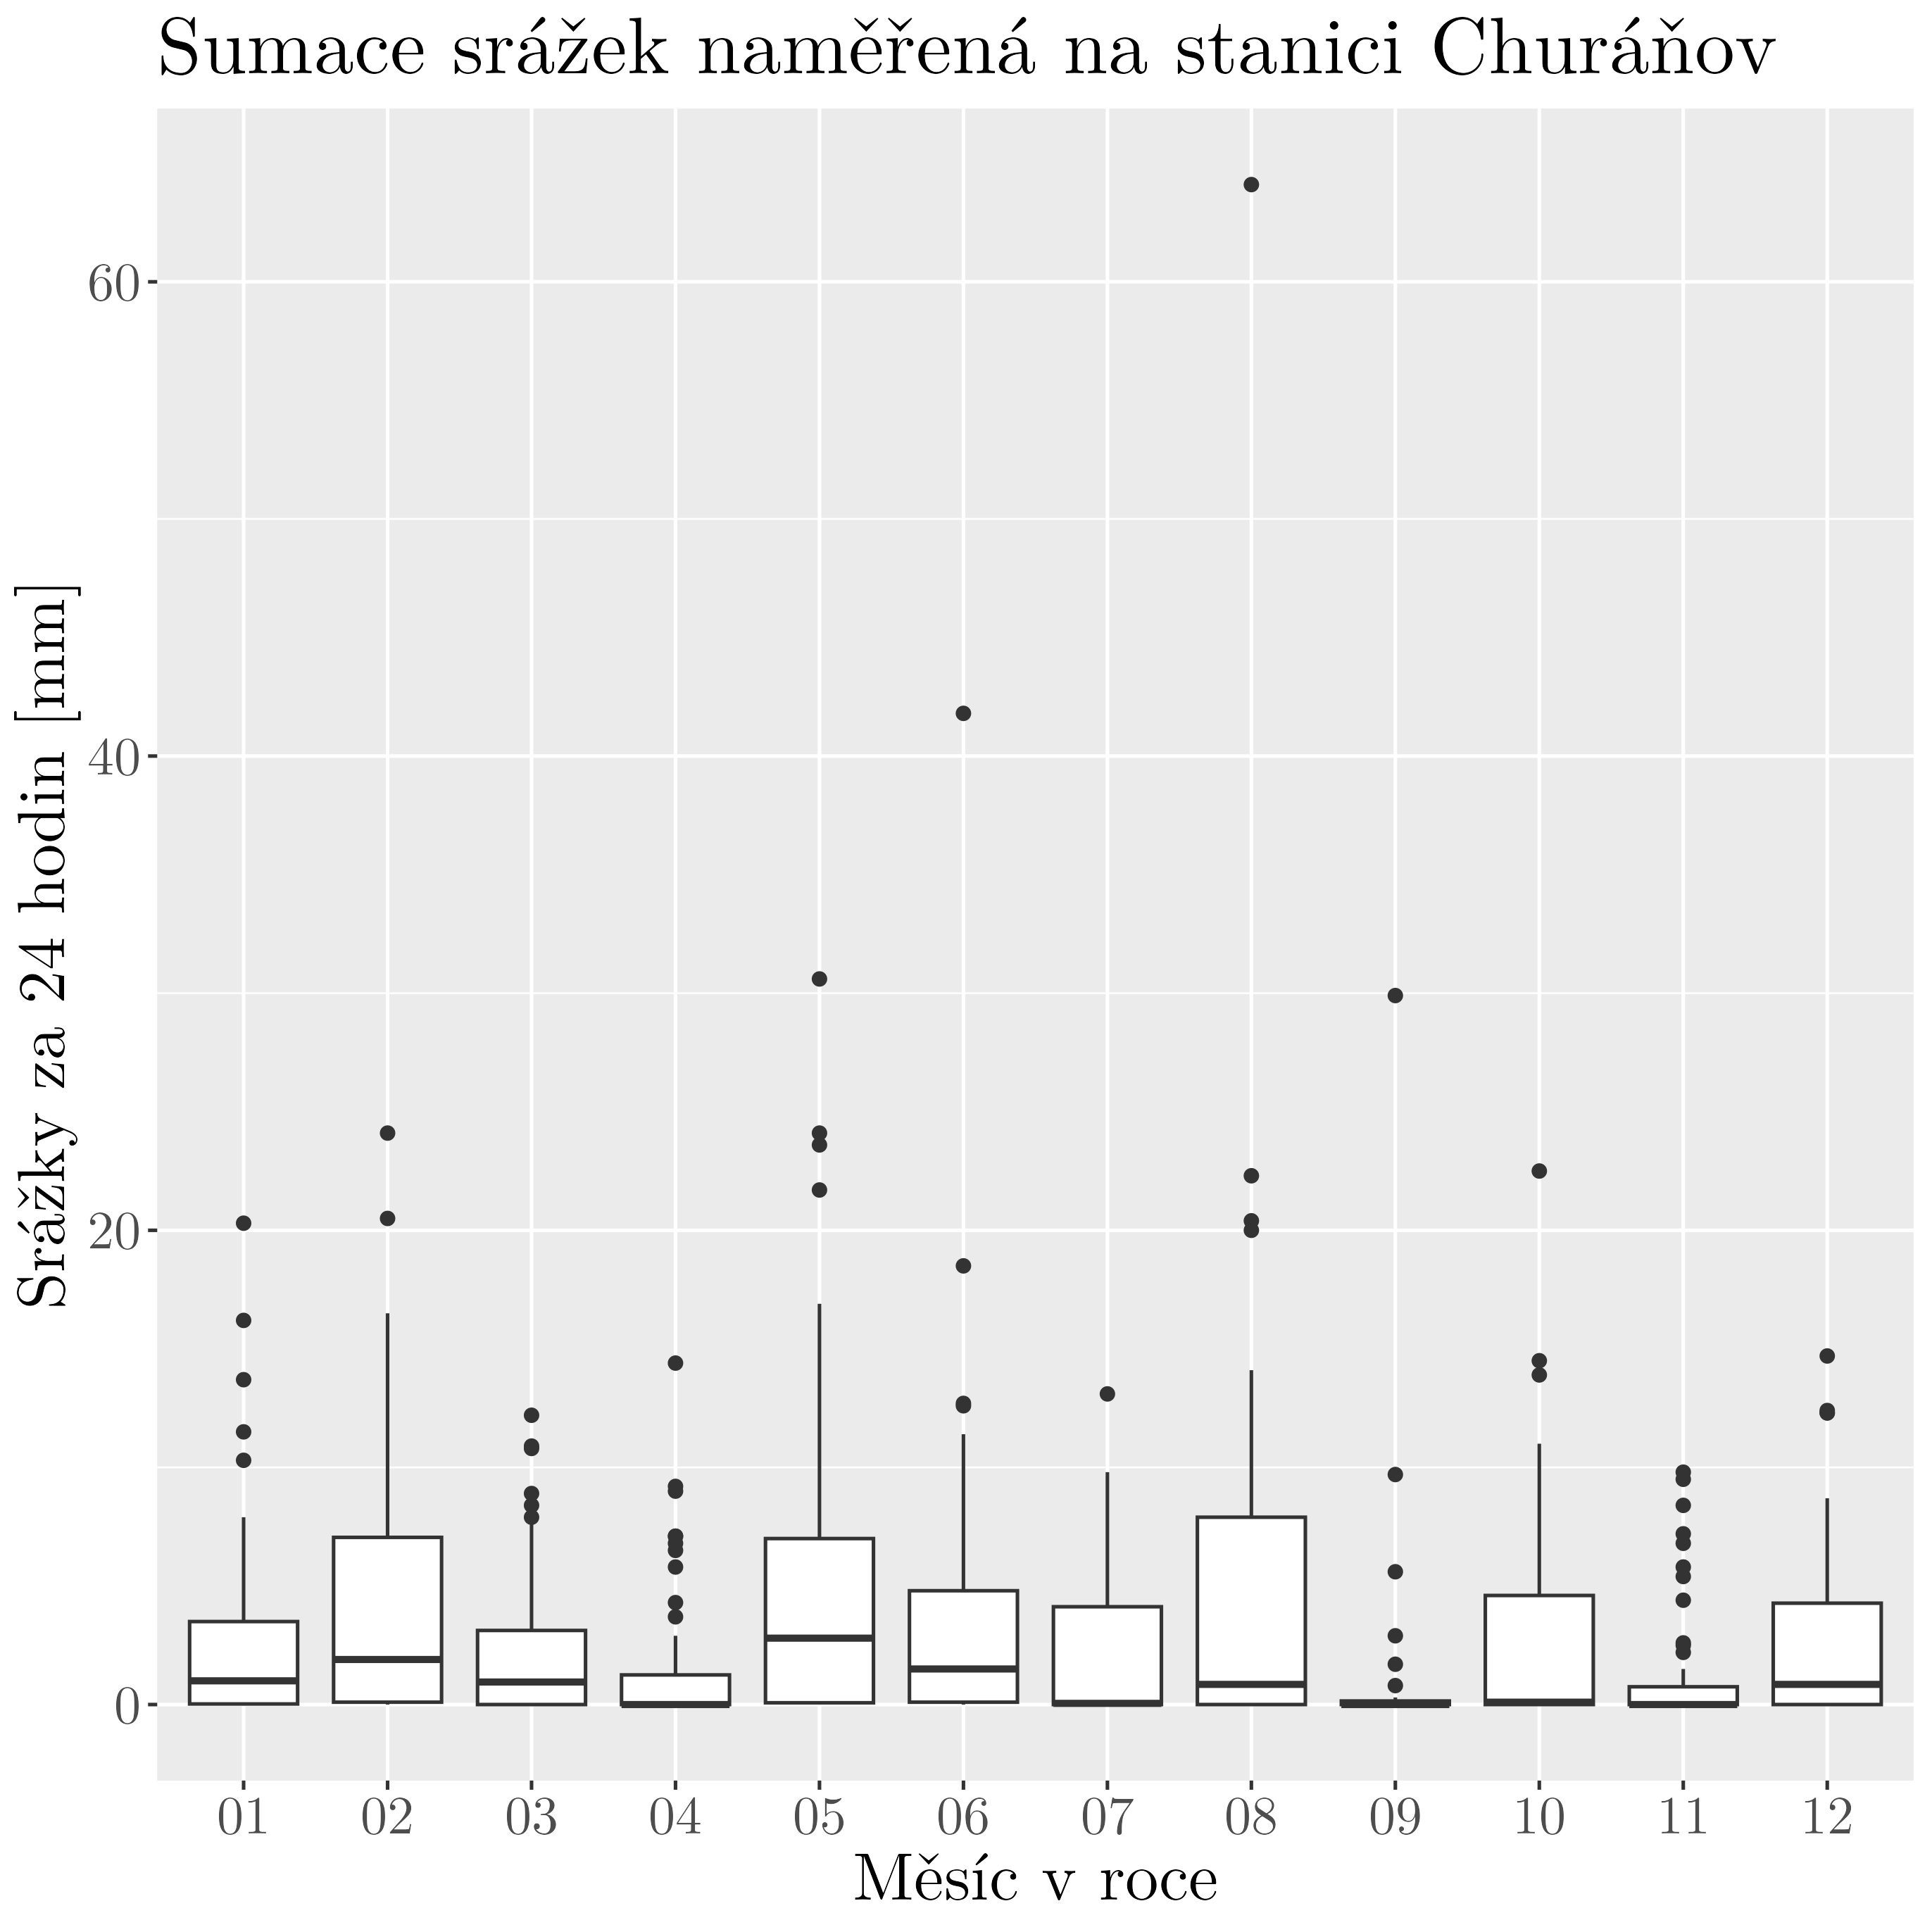
\includegraphics[width=\textwidth]{img/synop_prec.png}
		\caption{Denní suma srážek.}
		\label{fig:synop_prec}
	\end{subfigure}
	\hfill
	\begin{subfigure}{0.45\textwidth}
  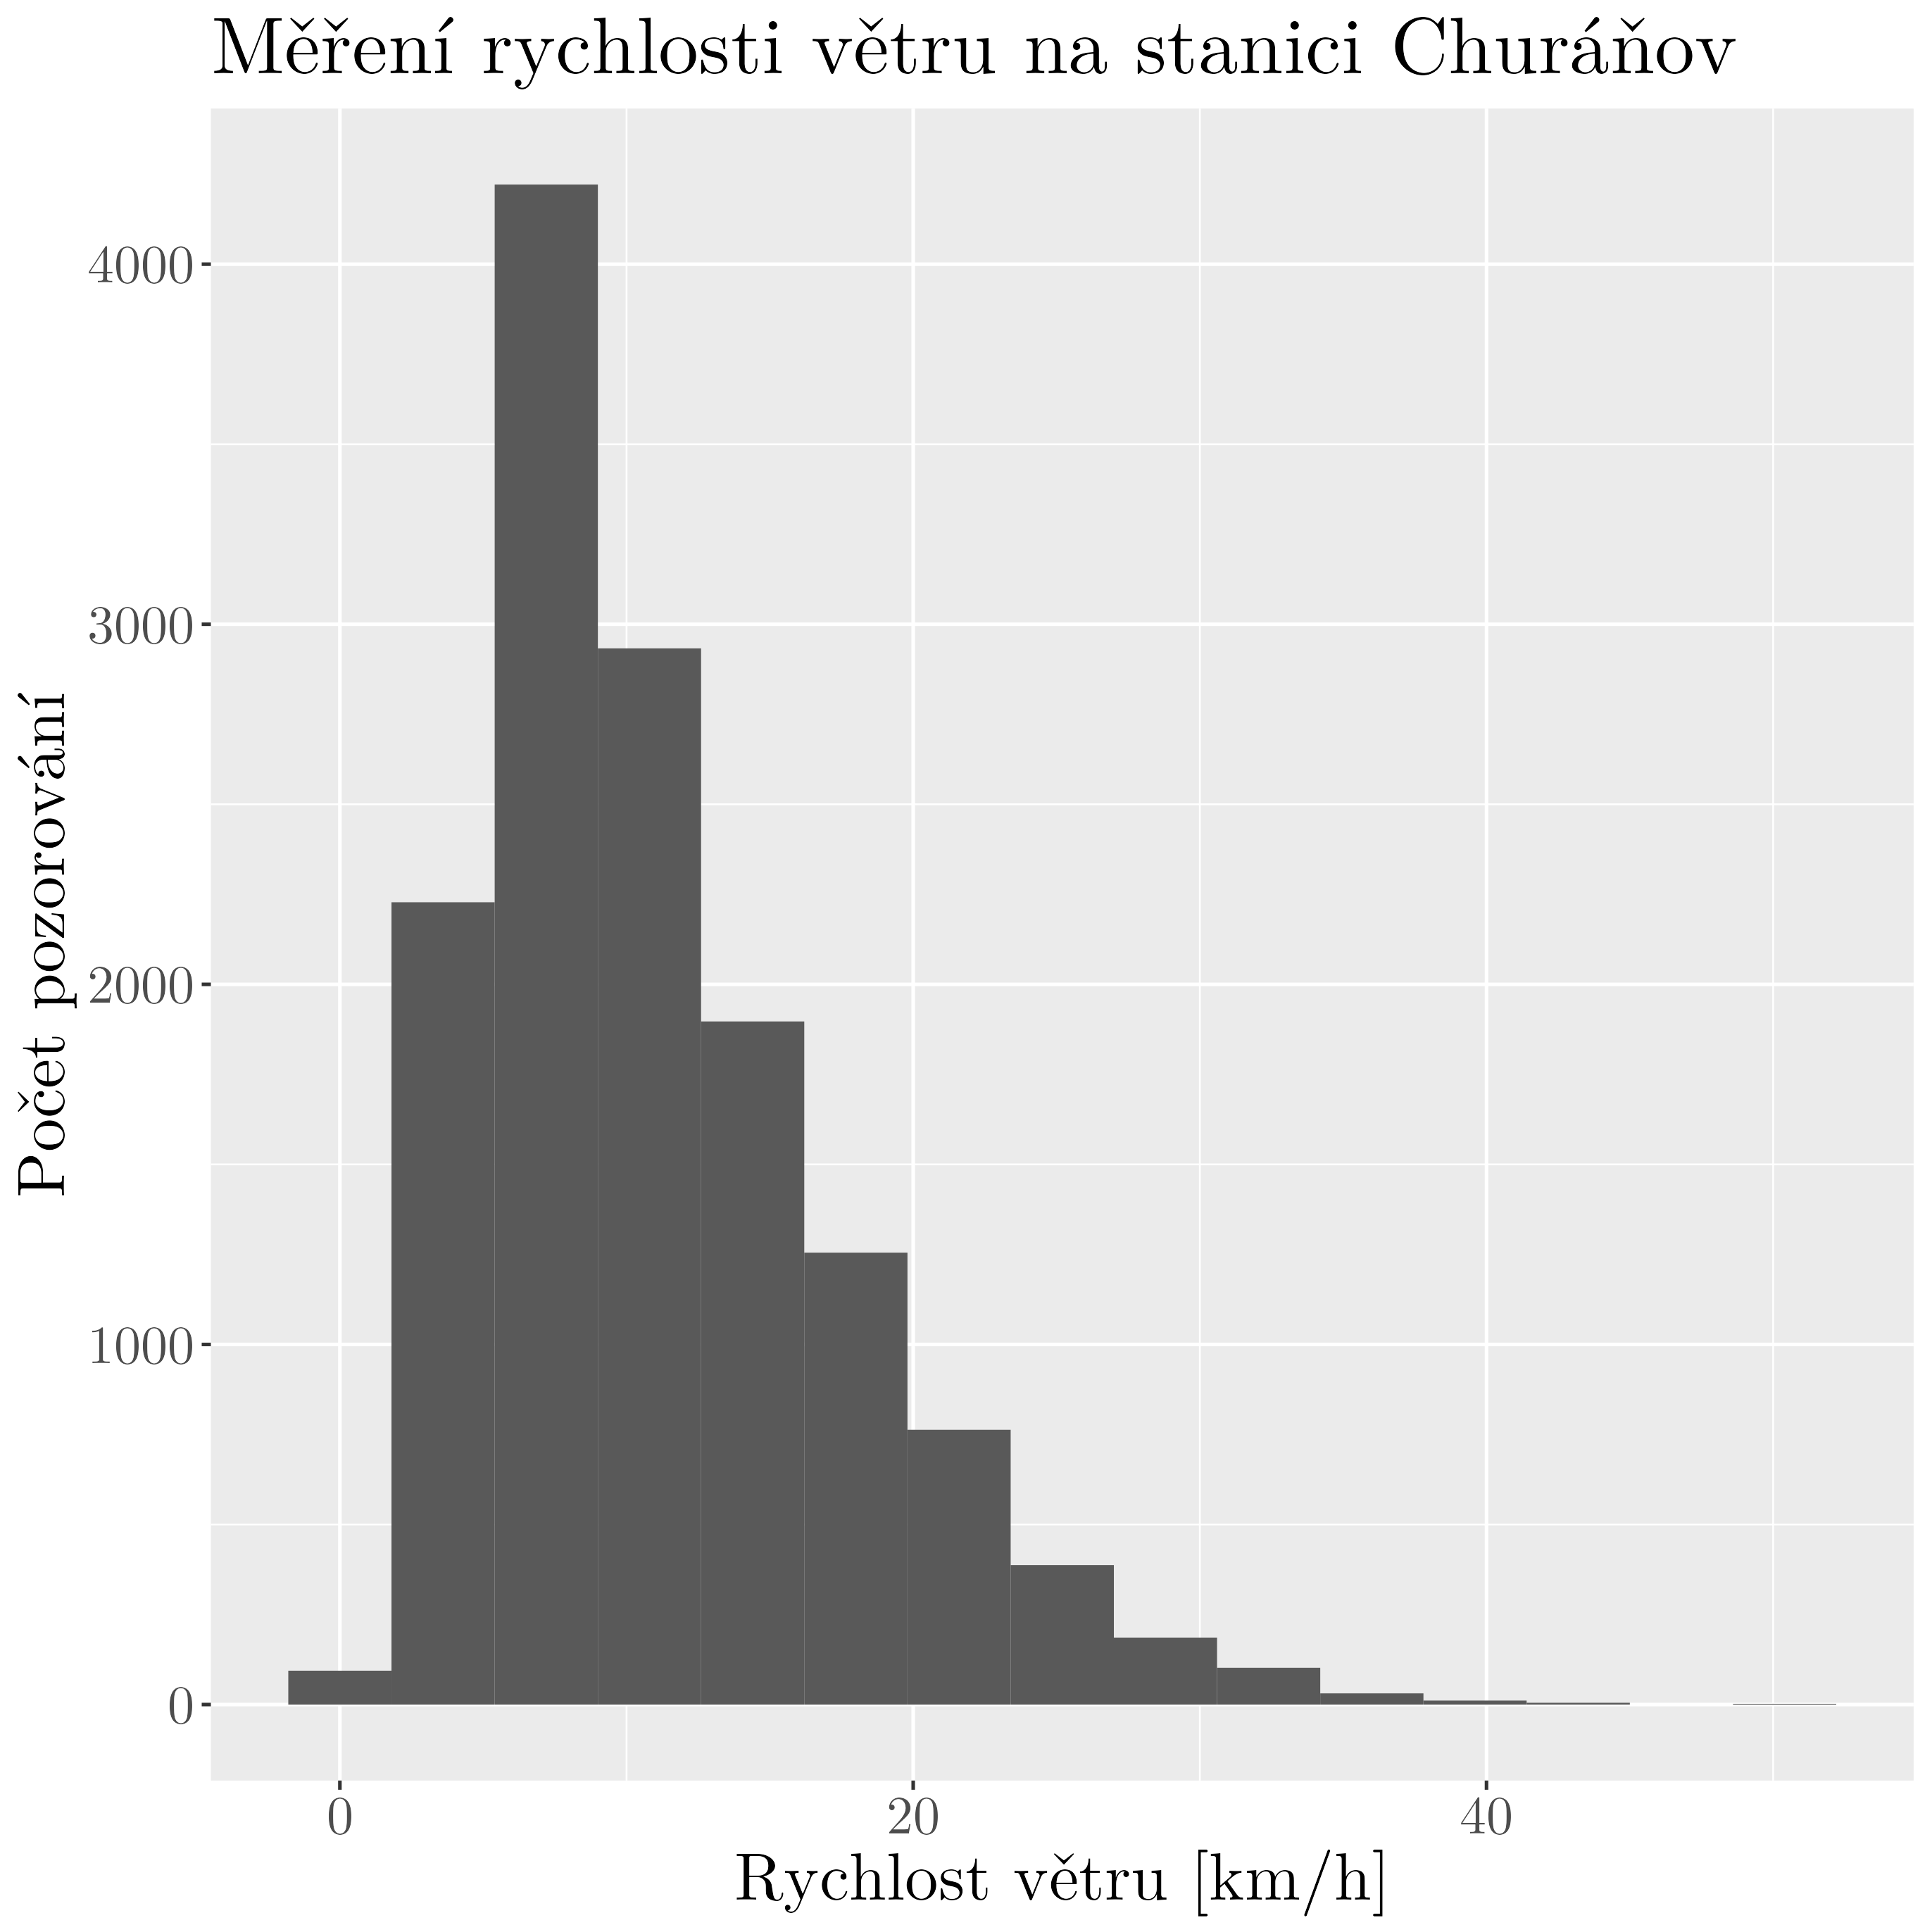
\includegraphics[width=\textwidth]{img/synop_ffkmh.png}
		\caption{Histogram pozorovaných okamžitých rychlostí větru.}
		\label{fig:synop_ffkmh}
	\end{subfigure}
	\caption{Data ze synoptické stanice Churáňov za období 12.10.2019 až 20.5.2021. Rychlost větru zobrazujeme jako obyčejný histogram, protože jde o informativnější graf než dělení podle měsíců v roce.}
	\label{fig:chmuukazka}
\end{figure}

Meteorologická stanice Churáňov měřící podle principů popsaných v kapitole \ref{chap:meteostations}. Stanice zaznamenává oblačnost každou hodinu od 6:00 do 20:00 UTC. Maximální teploty jsou typicky dosažené během dne, kdy většinou oblačnost známe. Například v zimě pod sněhem může ale maximální denní teplota být dosažena i v noci. Minimální denní teploty na druhou stranu typicky nastávají během ranních hodin, po východu Slunce, ale ojediněle i před ním (viz kapitola \ref{chap:showingoffdata} a obrázek \ref{fig:hours}). Pro minimální teploty nám tedy často chybí údaj o oblačnosti. Vyřazení těchto hodnot by vložilo velké zkreslení do dat, tudíž jsme se rozhodli využít data z projektu ERA5.

Pro každou hodnotu, která chybí ze staničního měření použijeme nejbližší hodnotu z ERA5 a to konkrétně z $\SI{49}{\degree}$ severní šířky a $\SI{13.5}{\degree}$ východní délky. Tato data byla vzdálená od stanice Churáňov $\SI{14.8}{km}$. V kapitole \ref{chap:disc_era5} budeme diskutovat vliv nahrazení dat pomocí ERA5.

\section{Data z Botanického ústavu Akademie věd}\label{chap:data_buav}
Data poskytnutá Botanickým ústavem Akademie věd České republiky byla naměřená dvěma typy čidel popsanými v kapitole \ref{chap:loggers}. Nadále se budeme zabývat pouze těmi plochami, které jsou opatřeny jak pozemními čidly, tak čidly ve standartní výšce $\SI{2}{m}$. Na obrázku \ref{fig:rozlozenicidel} můžeme vidět jejich prostorové rozložení, celkově jde o 157 čidel. 

Umístění čidel bylo vybíráno tak, aby pokryly gradienty nadmořské výšky (5 tříd), potenciální solární radiace, určující množství záření, které dopadá na zem (3 třídy) a topografického vlhkostního indexu, který kombinuje svažitost a akumulaci vody v terénu (3 třídy). Plochy byly dále doplněny tak, aby bylo rovnoměrně pokryto území národních parků, a aby se nevyskytovaly poblíž turistických stezek.

\begin{figure}
	\centering
	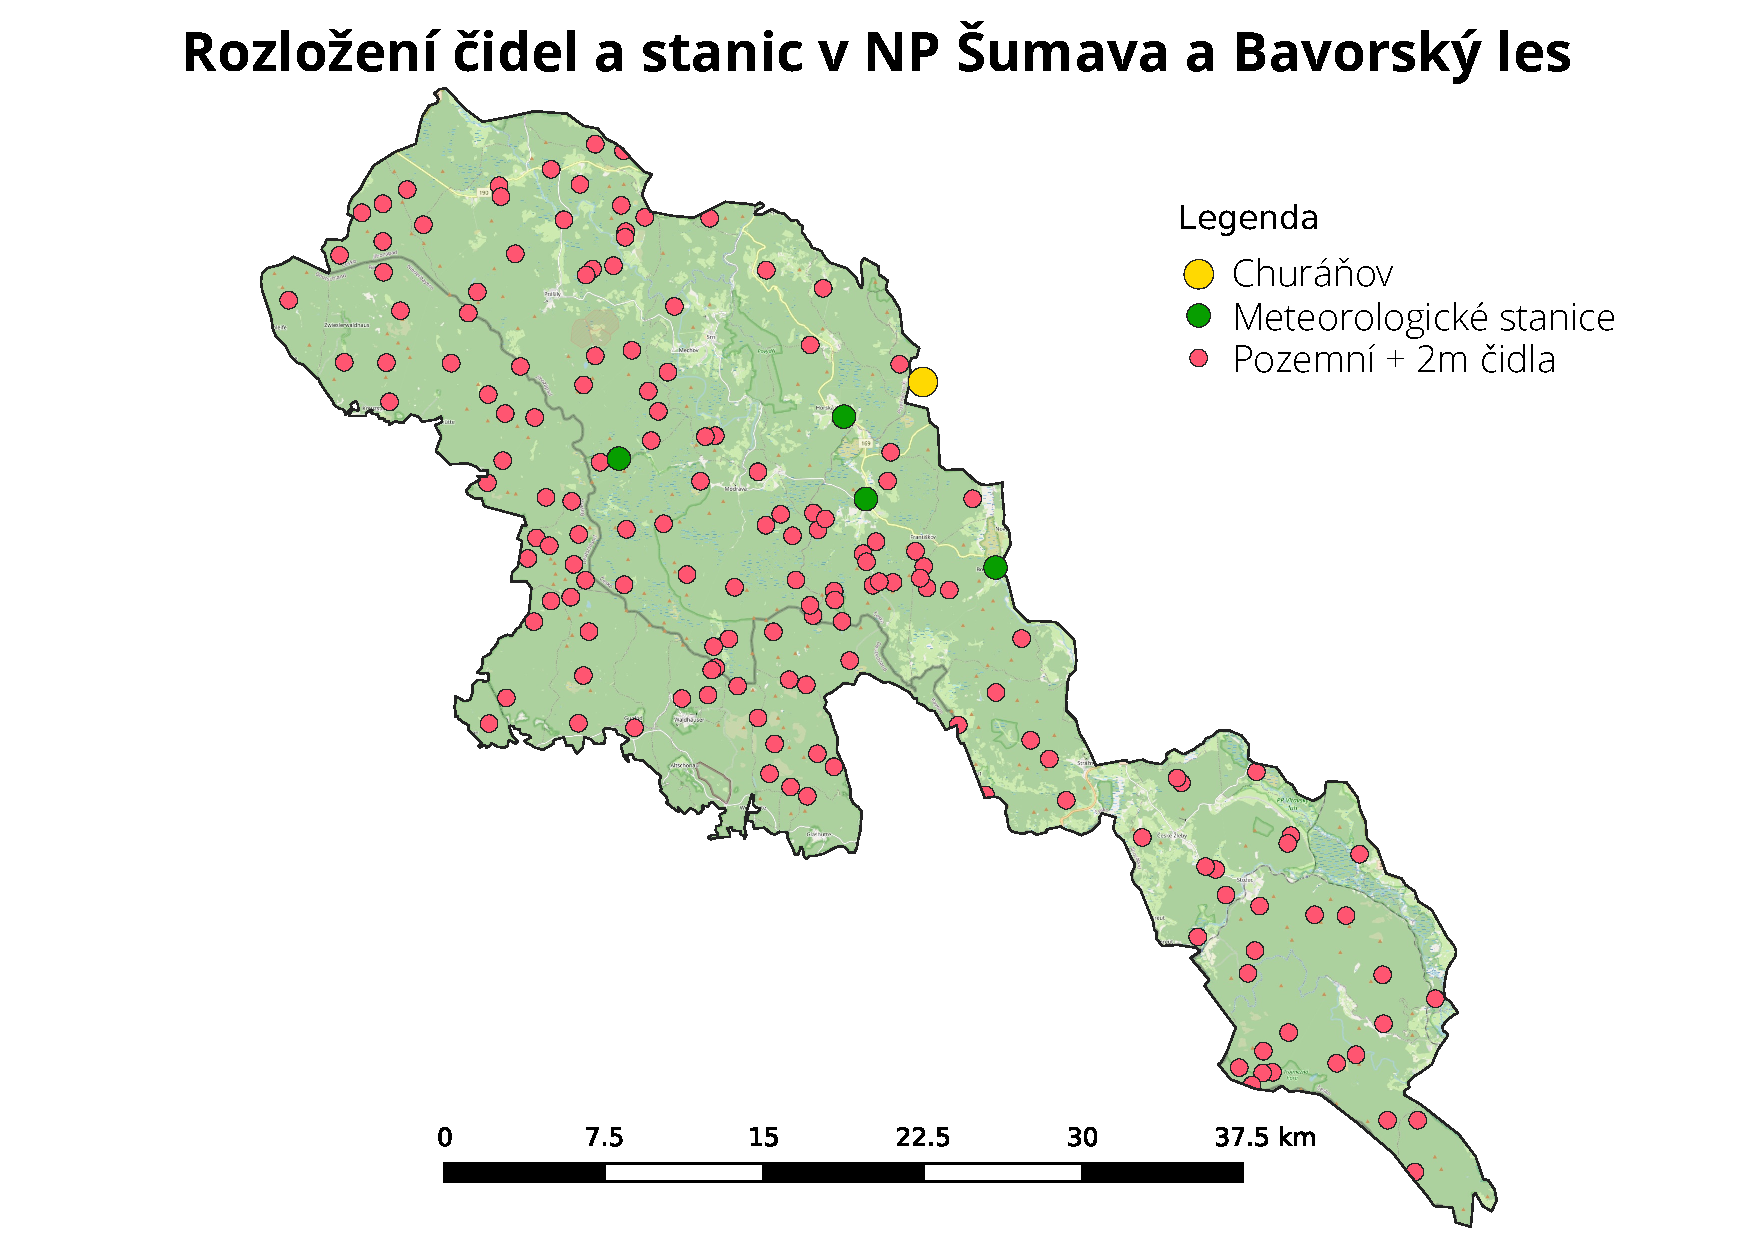
\includegraphics[width=0.95\textwidth]{img/rozlozenicidel.pdf}
	\caption{Rozložení čidel a meteorologický stanic v Národním parku Šumava ($N=112$) a Národním parku Bavorský les ($N=45$)}
	\label{fig:rozlozenicidel}
\end{figure}

Data vykazují malou chybovost, duplicitní a chybějící záznamy byly vyřazeny. Dále byla data vizuálně překontrolována, jestli neobsahují očividně chybná data. Části, kdy byla čidla např. povytažená ze země (pozná se podle hodnot půdní vlhkosti), byly nahrazeny hodnotami NA. Podobně pokud čidlo T1 spadlo ze stromu, tak jsou hodnoty nahrazeny NA. Toto čištění dat provedli RNDr. Josef Brůna, Ph.D., doc. Ing. Jan Wild, Ph.D. a další, s jejichž svolením jsou data využitá v této práci. Ve velmi ojedinělých případech chyběly odpovídající hodnoty teplot ve $\SI{2}{m}$, v době, kdy při zemi nastalo denní maximum nebo minimum. Pokud existovaly hodnoty až 30 minut starší, tak jsme použili tyto, v opačném případě jsme čidlo pro daný den vyřadili, šlo o jednotky případů.

Dostupnost dat z čidel je vidět na obrázku \ref{fig:dostupnostdat}, vidíme zde dvě skupiny čidel. Čidla nacházející se v Národním parku Bavorský les mají dostupná data pro cca 400 dnů. Čidla z Národního parku Šumava mají dostupná data pro téměř 600 dnů. Na obrázku \ref{fig:dostupnostdnu} vidíme, na kolika čidlech jsou zastoupeny jednotlivé dny.

\begin{figure}
	\centering
	\begin{subfigure}{0.45\textwidth}
  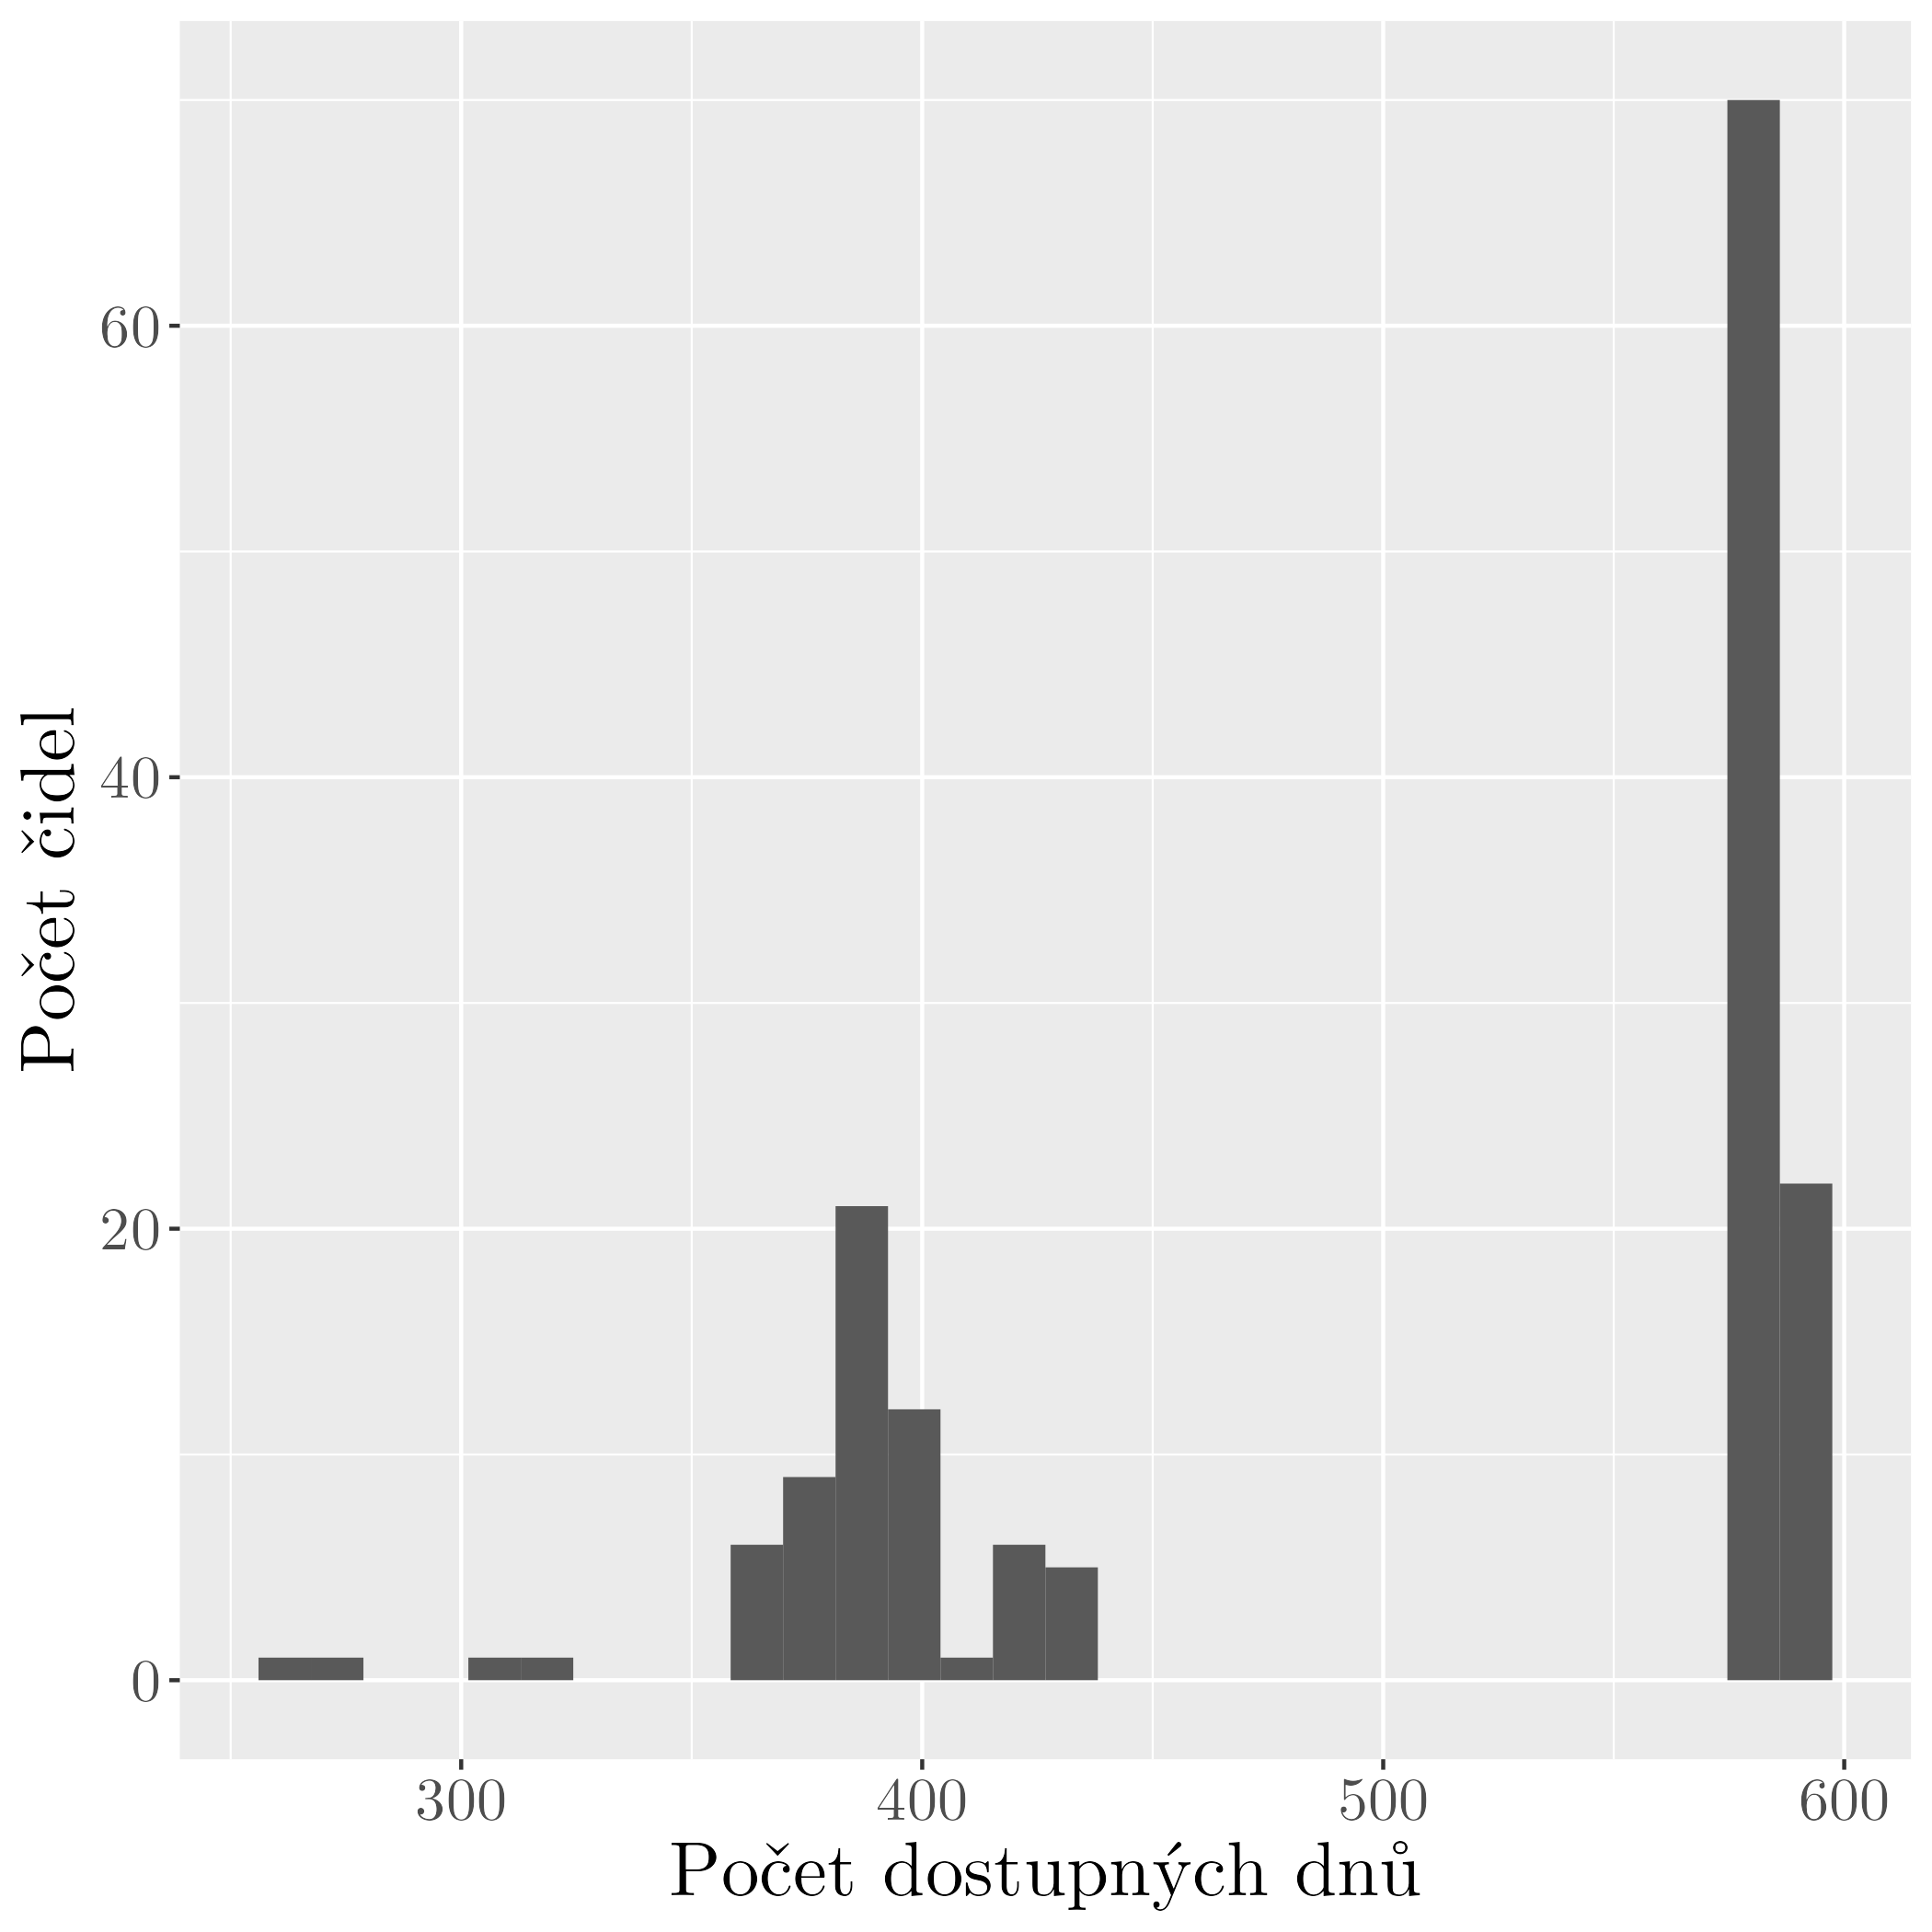
\includegraphics[width=\textwidth]{img/hist_numofdayavailability.png}
	\caption{Histogram ukazující množství dostupných dnů pro jednotlivá čidla}
	\label{fig:dostupnostdat}
	\end{subfigure}
	\hfill
	\begin{subfigure}{0.45\textwidth}
  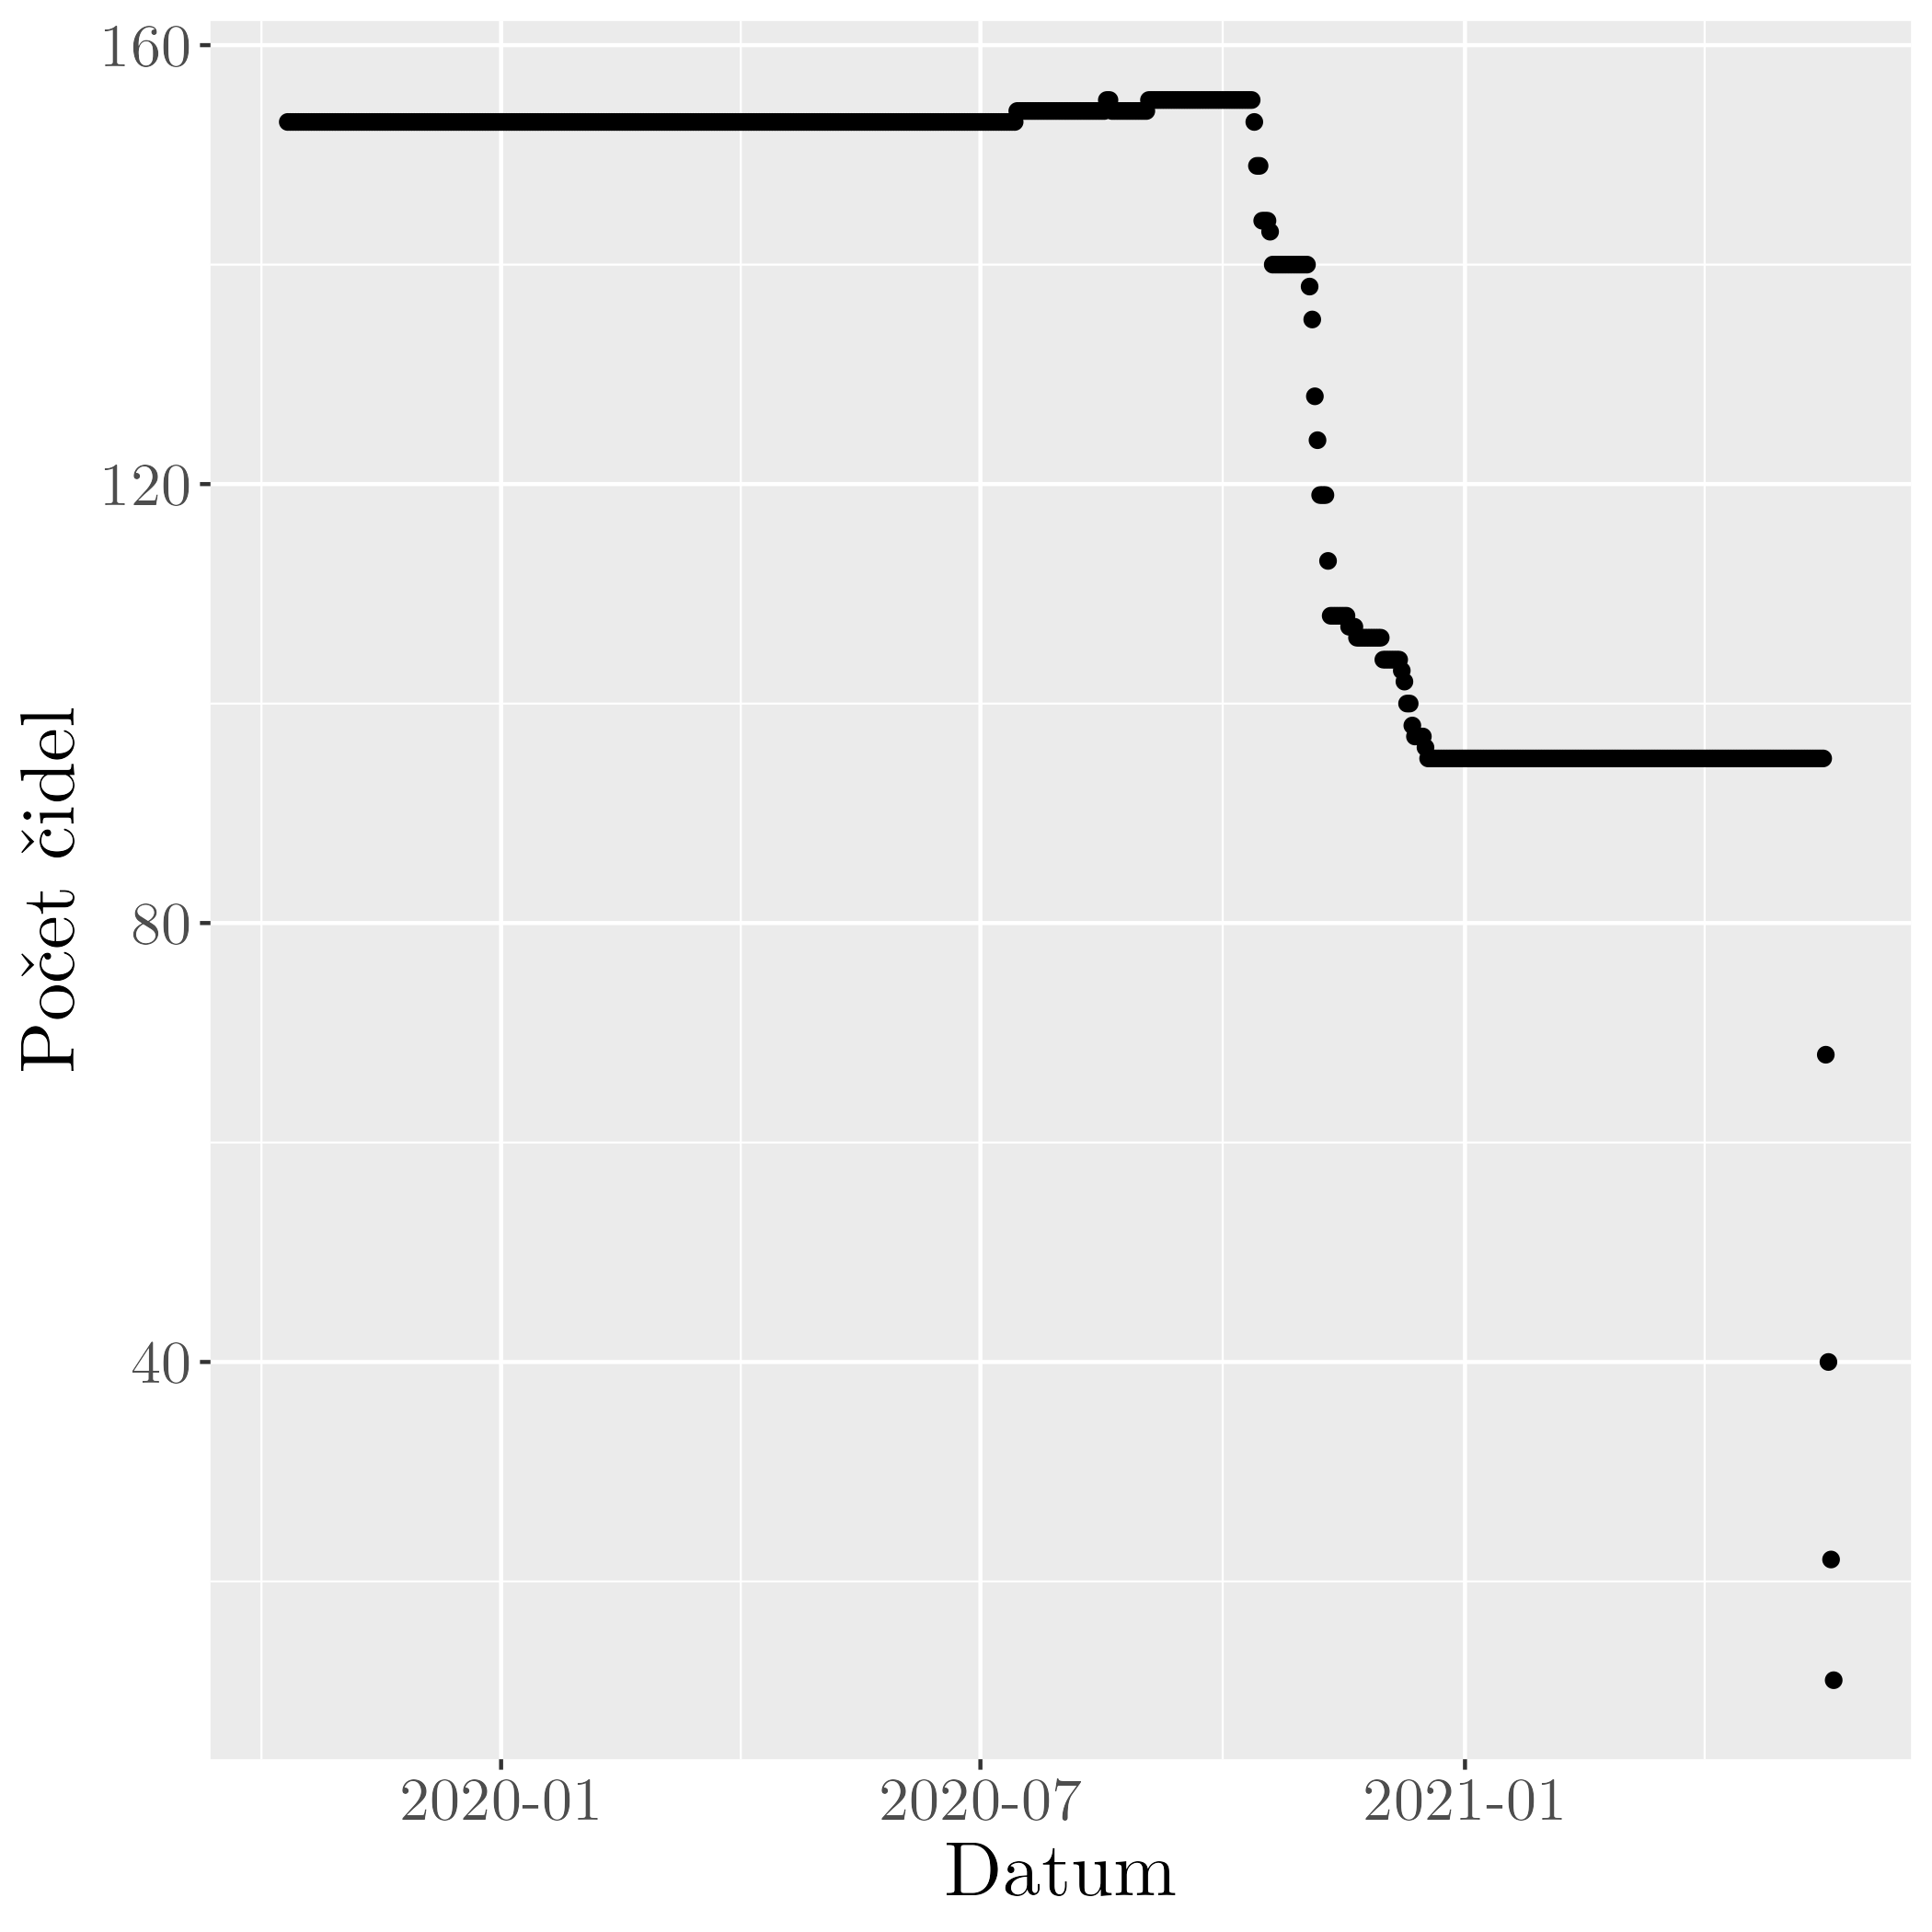
\includegraphics[width=\textwidth]{img/date_availability.png}
	\caption{Graf zastoupení čidel pro jednotlivé dny}
	\label{fig:dostupnostdnu}
	\end{subfigure}
	\caption{Dostupnost dat z čidel}
\end{figure}

Pro samotné zpracování jsme vyřadili poslední 4 dny v květnu, kvůli nižšímu počtu aktivních čidel. Tímto se dostáváme na interval dat od 12.10.2019 do 17.5.2021.

\section{Insolace}
Na obrázku \ref{fig:insolacelogger} můžeme vidět hodnoty insolace spočtené podle odstavce \ref{chap:insolation} pro čidlo, které je nejblíž stanici Churáňov. Sinusoida nám téměř určuje hodnotu maximální denní insolace. Maximum insolace většinou nastává dříve než maximální teploty. Dále také pracujeme na časovém měřítku 15 minut a je tedy malá pravděpodobnost, že nastane maximální denní teplota ve stejnou dobu jako maximální denní insolace. Nulové hodnoty odpovídají tomu, že denní maximální teplota nastala v noci, to způsobuje přítomnost sněhu v zimě.

\begin{figure}
	\centering
	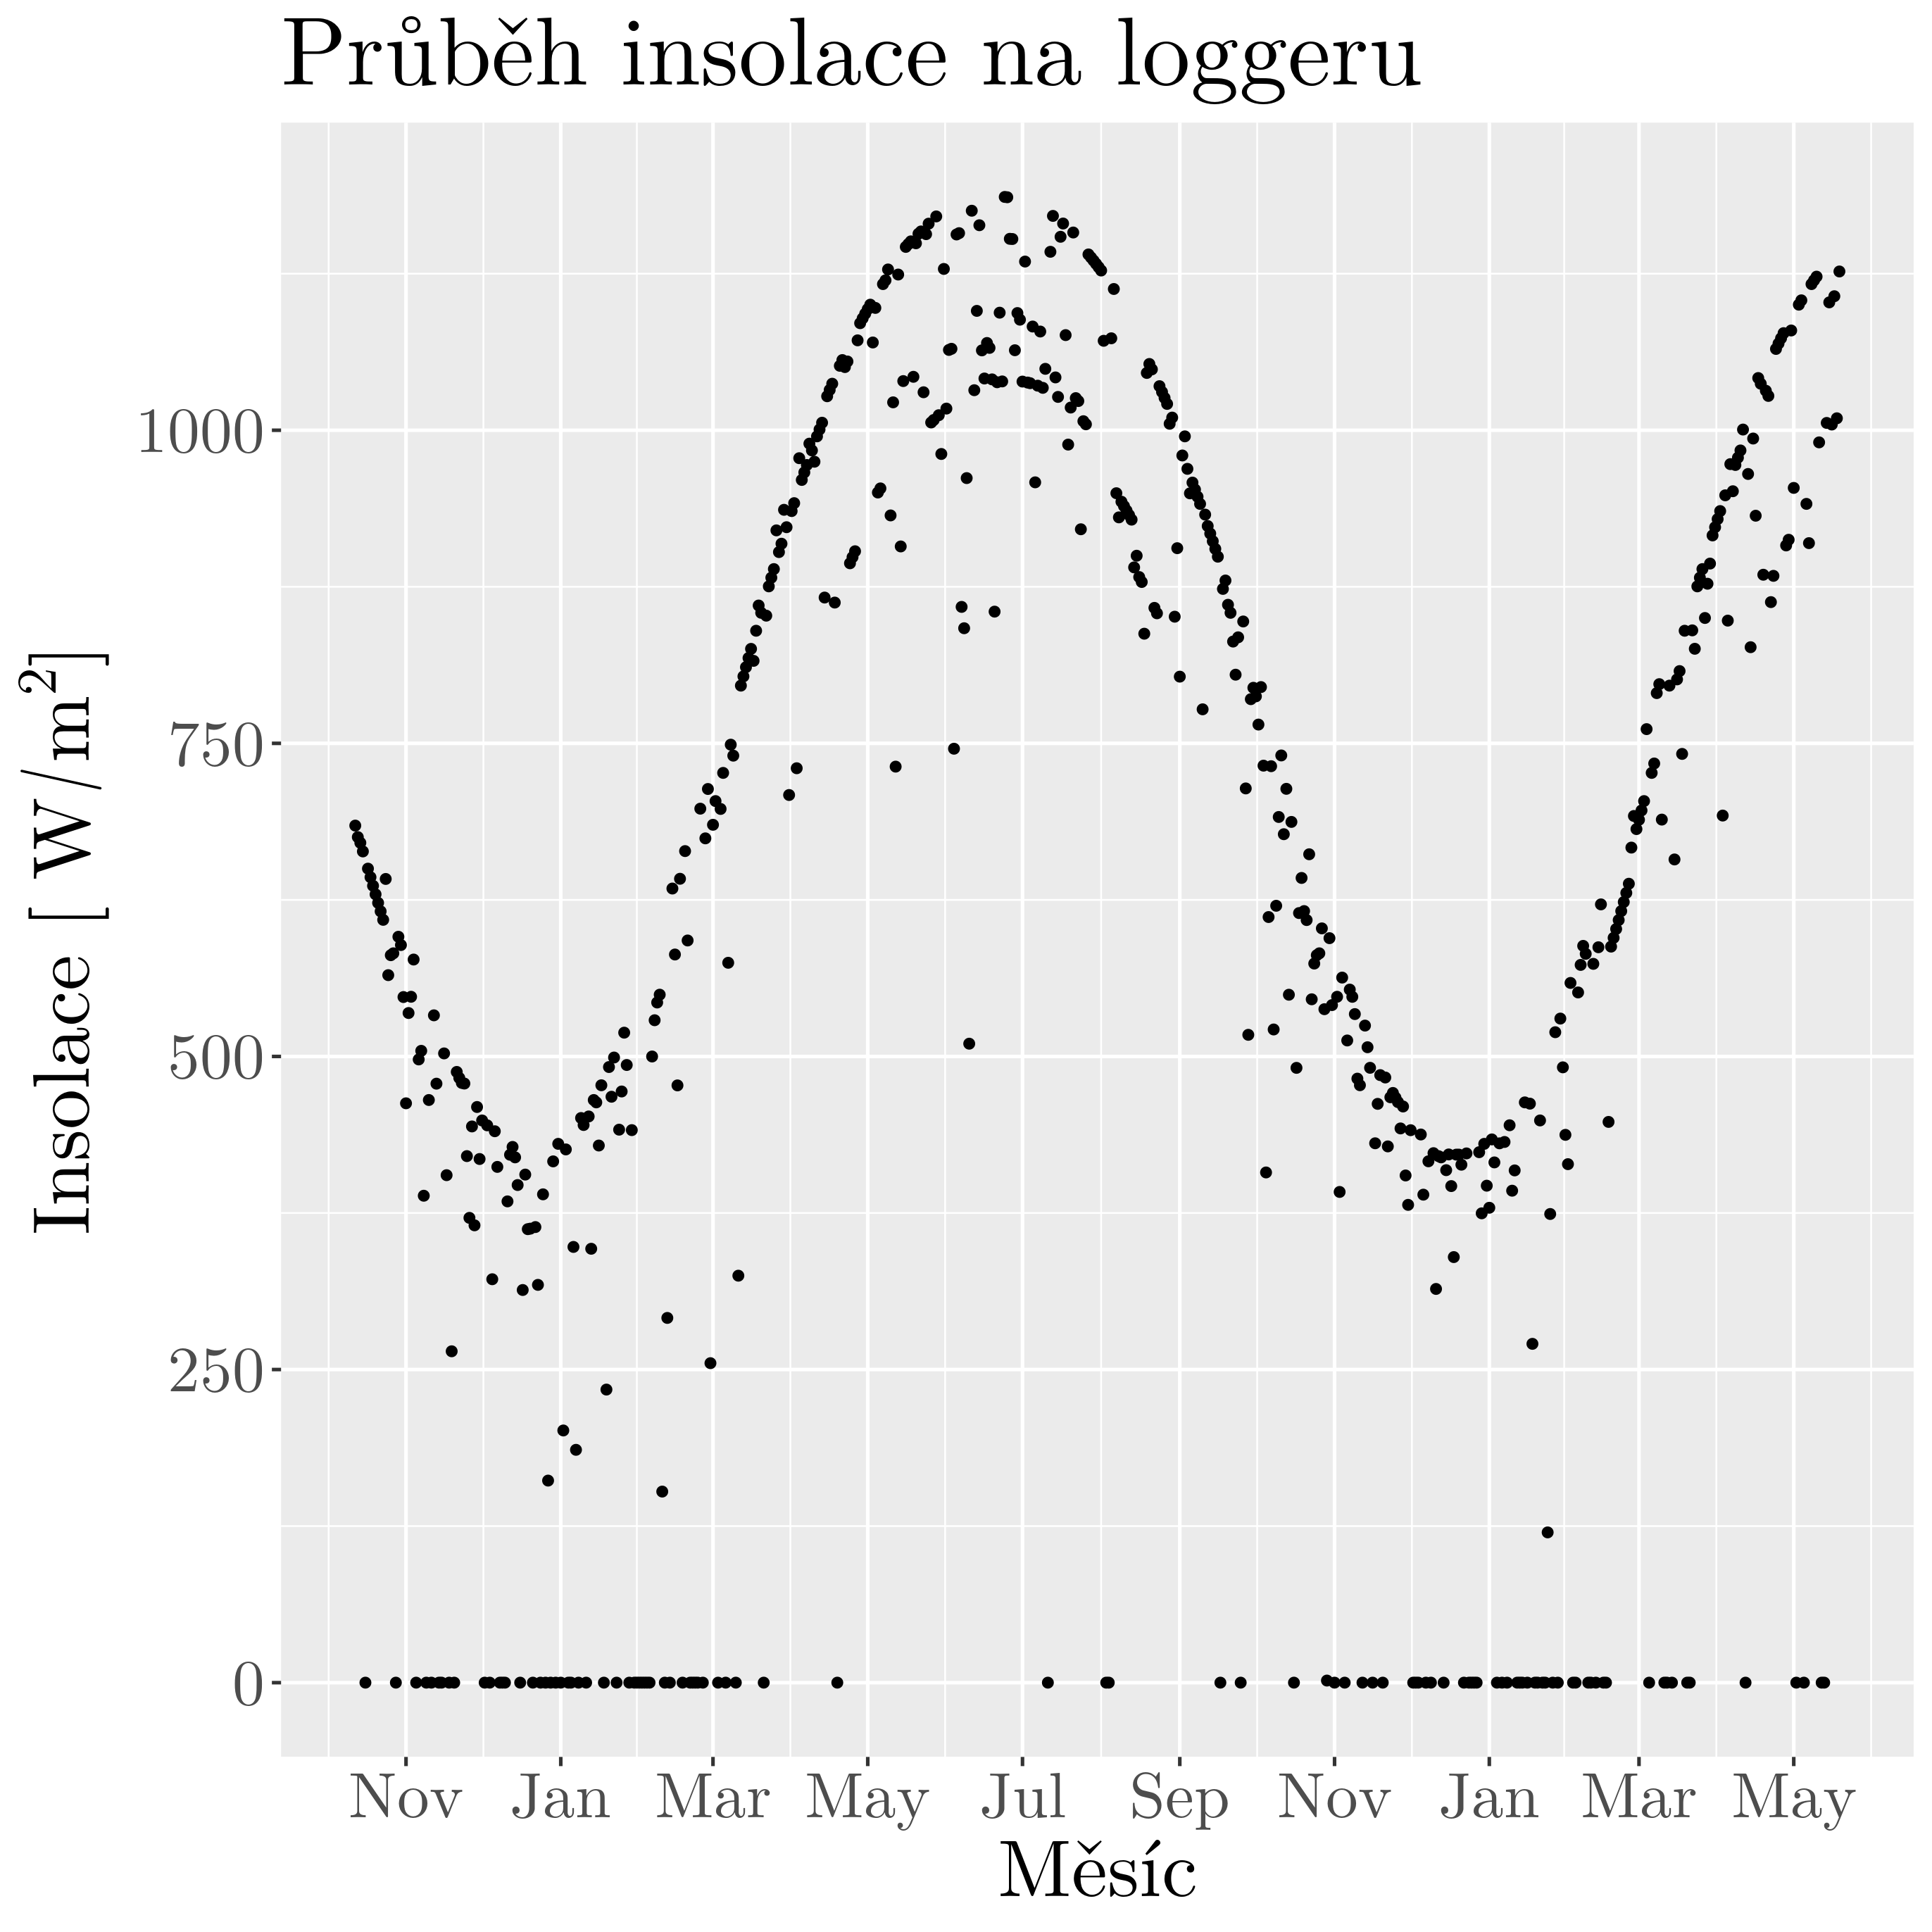
\includegraphics[width=0.65\textwidth]{img/ch2/insolation_max15cmNPS_4311_D_TMS.png}
	\caption{Hodnoty insolace na čidlu nejblíže stanici Churáňov v době dosažení maximální denní teploty ve výšce $\SI{15}{cm}$.}
	\label{fig:insolacelogger}
\end{figure}

\section{Ukázka použitých dat}\label{chap:showingoffdata}
Dále se podíváme na ukázku dat naměřených na čidlech. Na obrázcích \ref{fig:hours} můžeme vidět, kdy nastávaly maximální a minimální teploty ve výškách $\SI{0}{cm}$ a $\SI{15}{cm}$ nad zemí, denní hodina je uvedená v UTC, nikoliv SEČ nebo SELČ. U maximálních teplot si můžeme všimnout kromě maxima v době kolem 10 UTC také menšího maxima a odlehlých hodnot způsobených přítomností sněhu v zimě. Podobně měl sníh vliv i na dobu minimálních teplot v zimě.

\begin{figure}
	\centering
	\begin{subfigure}{0.45\textwidth}
  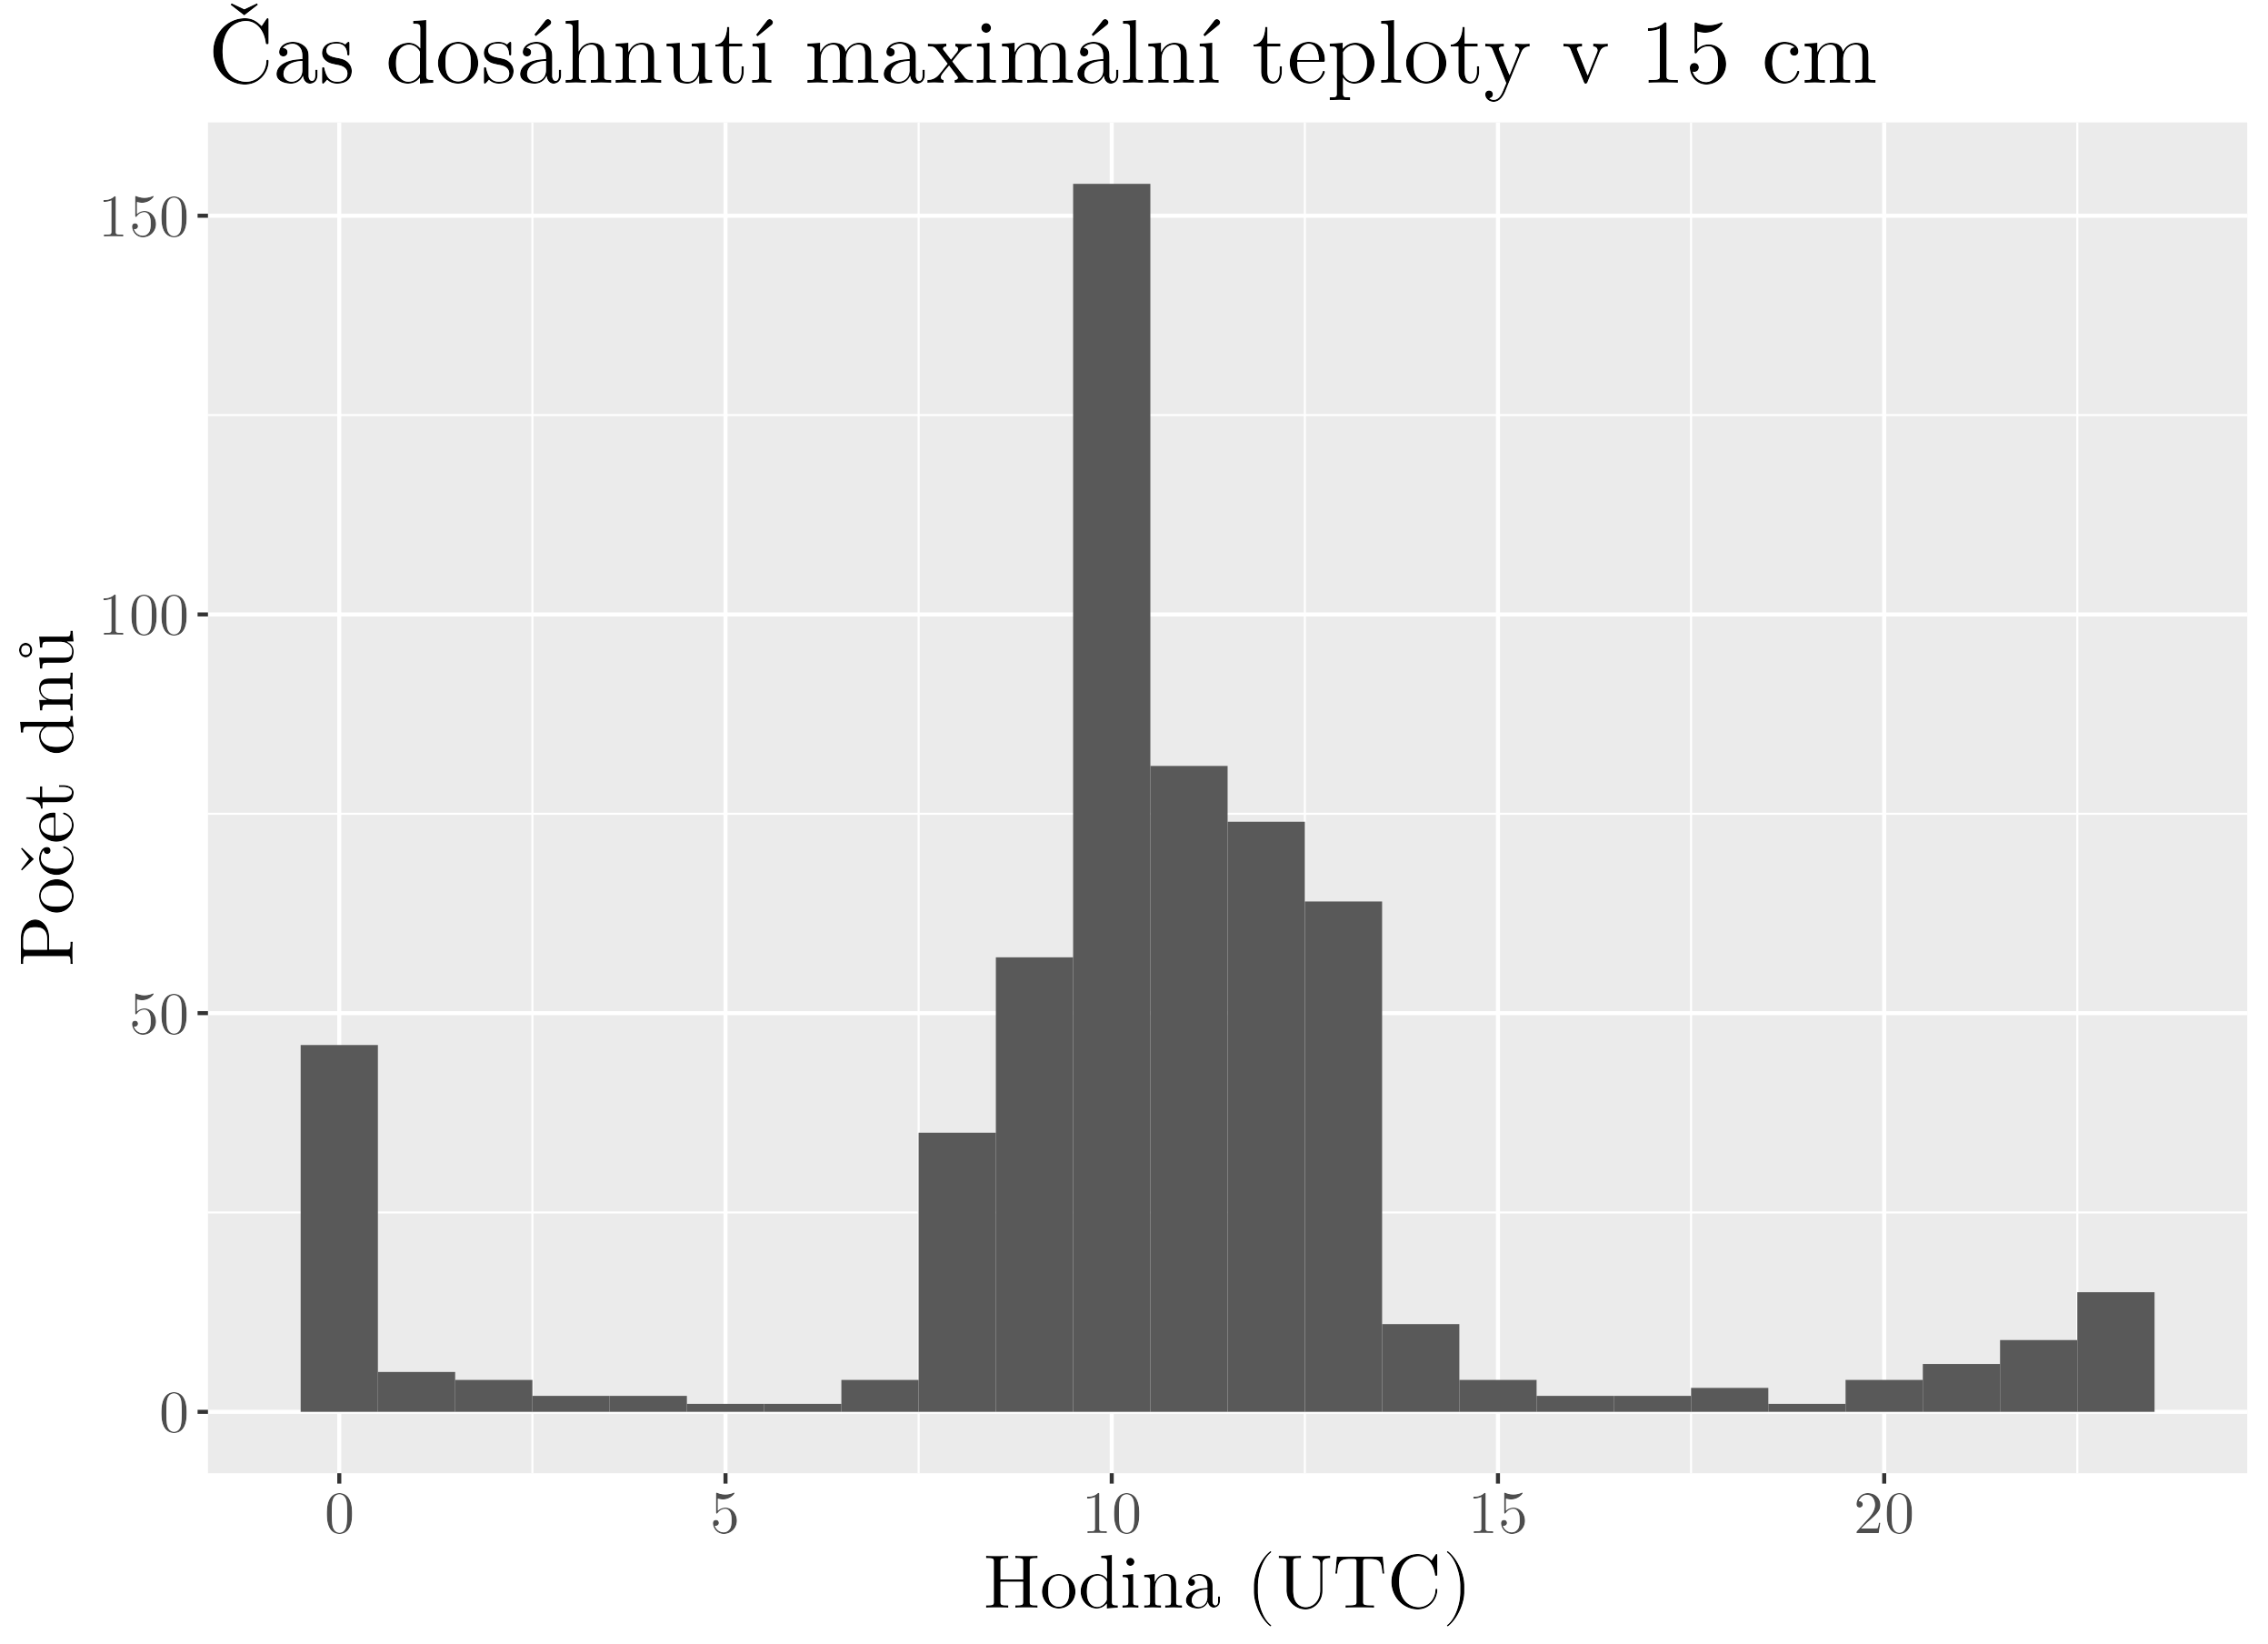
\includegraphics[width=\textwidth]{img/hist_hourmax15cm.png}
		\caption{}
		\label{fig:hourmax15cm}
	\end{subfigure}
	\hfill
	\begin{subfigure}{0.45\textwidth}
  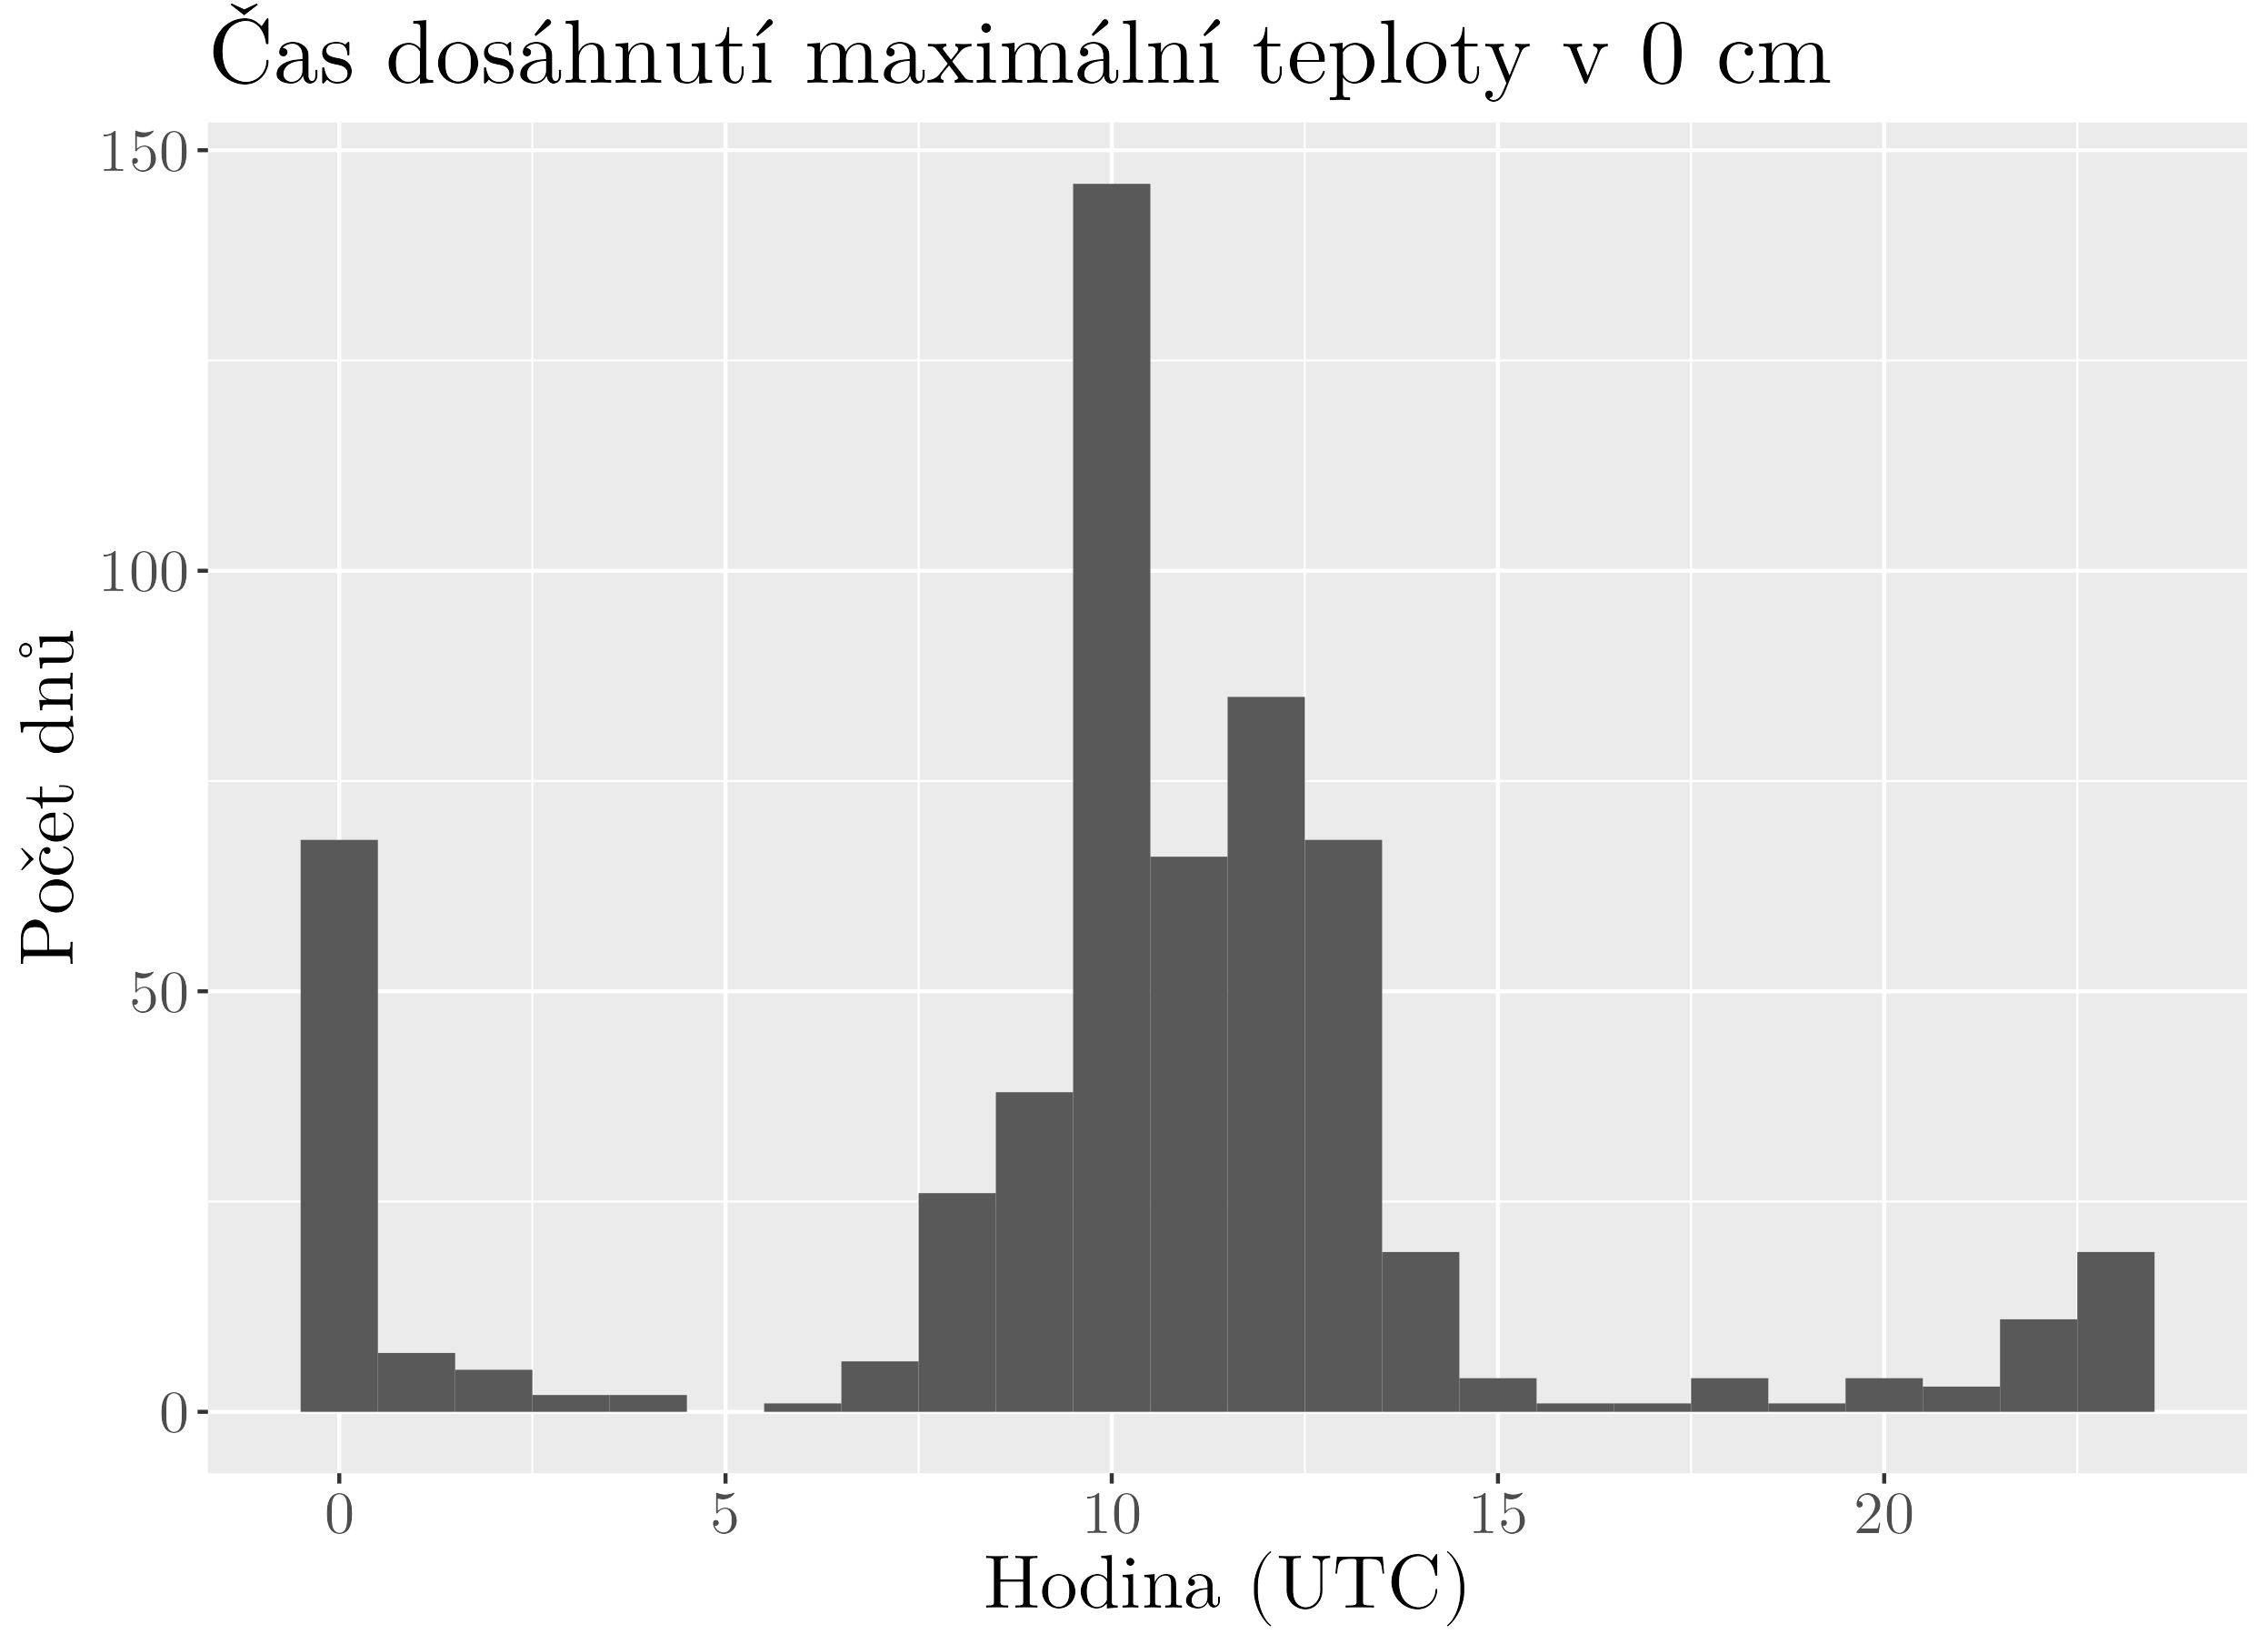
\includegraphics[width=\textwidth]{img/hist_hourmax0cm.png}
		\caption{}
		\label{fig:hourmax0cm}
	\end{subfigure}
	\hfill
	\begin{subfigure}{0.45\textwidth}
  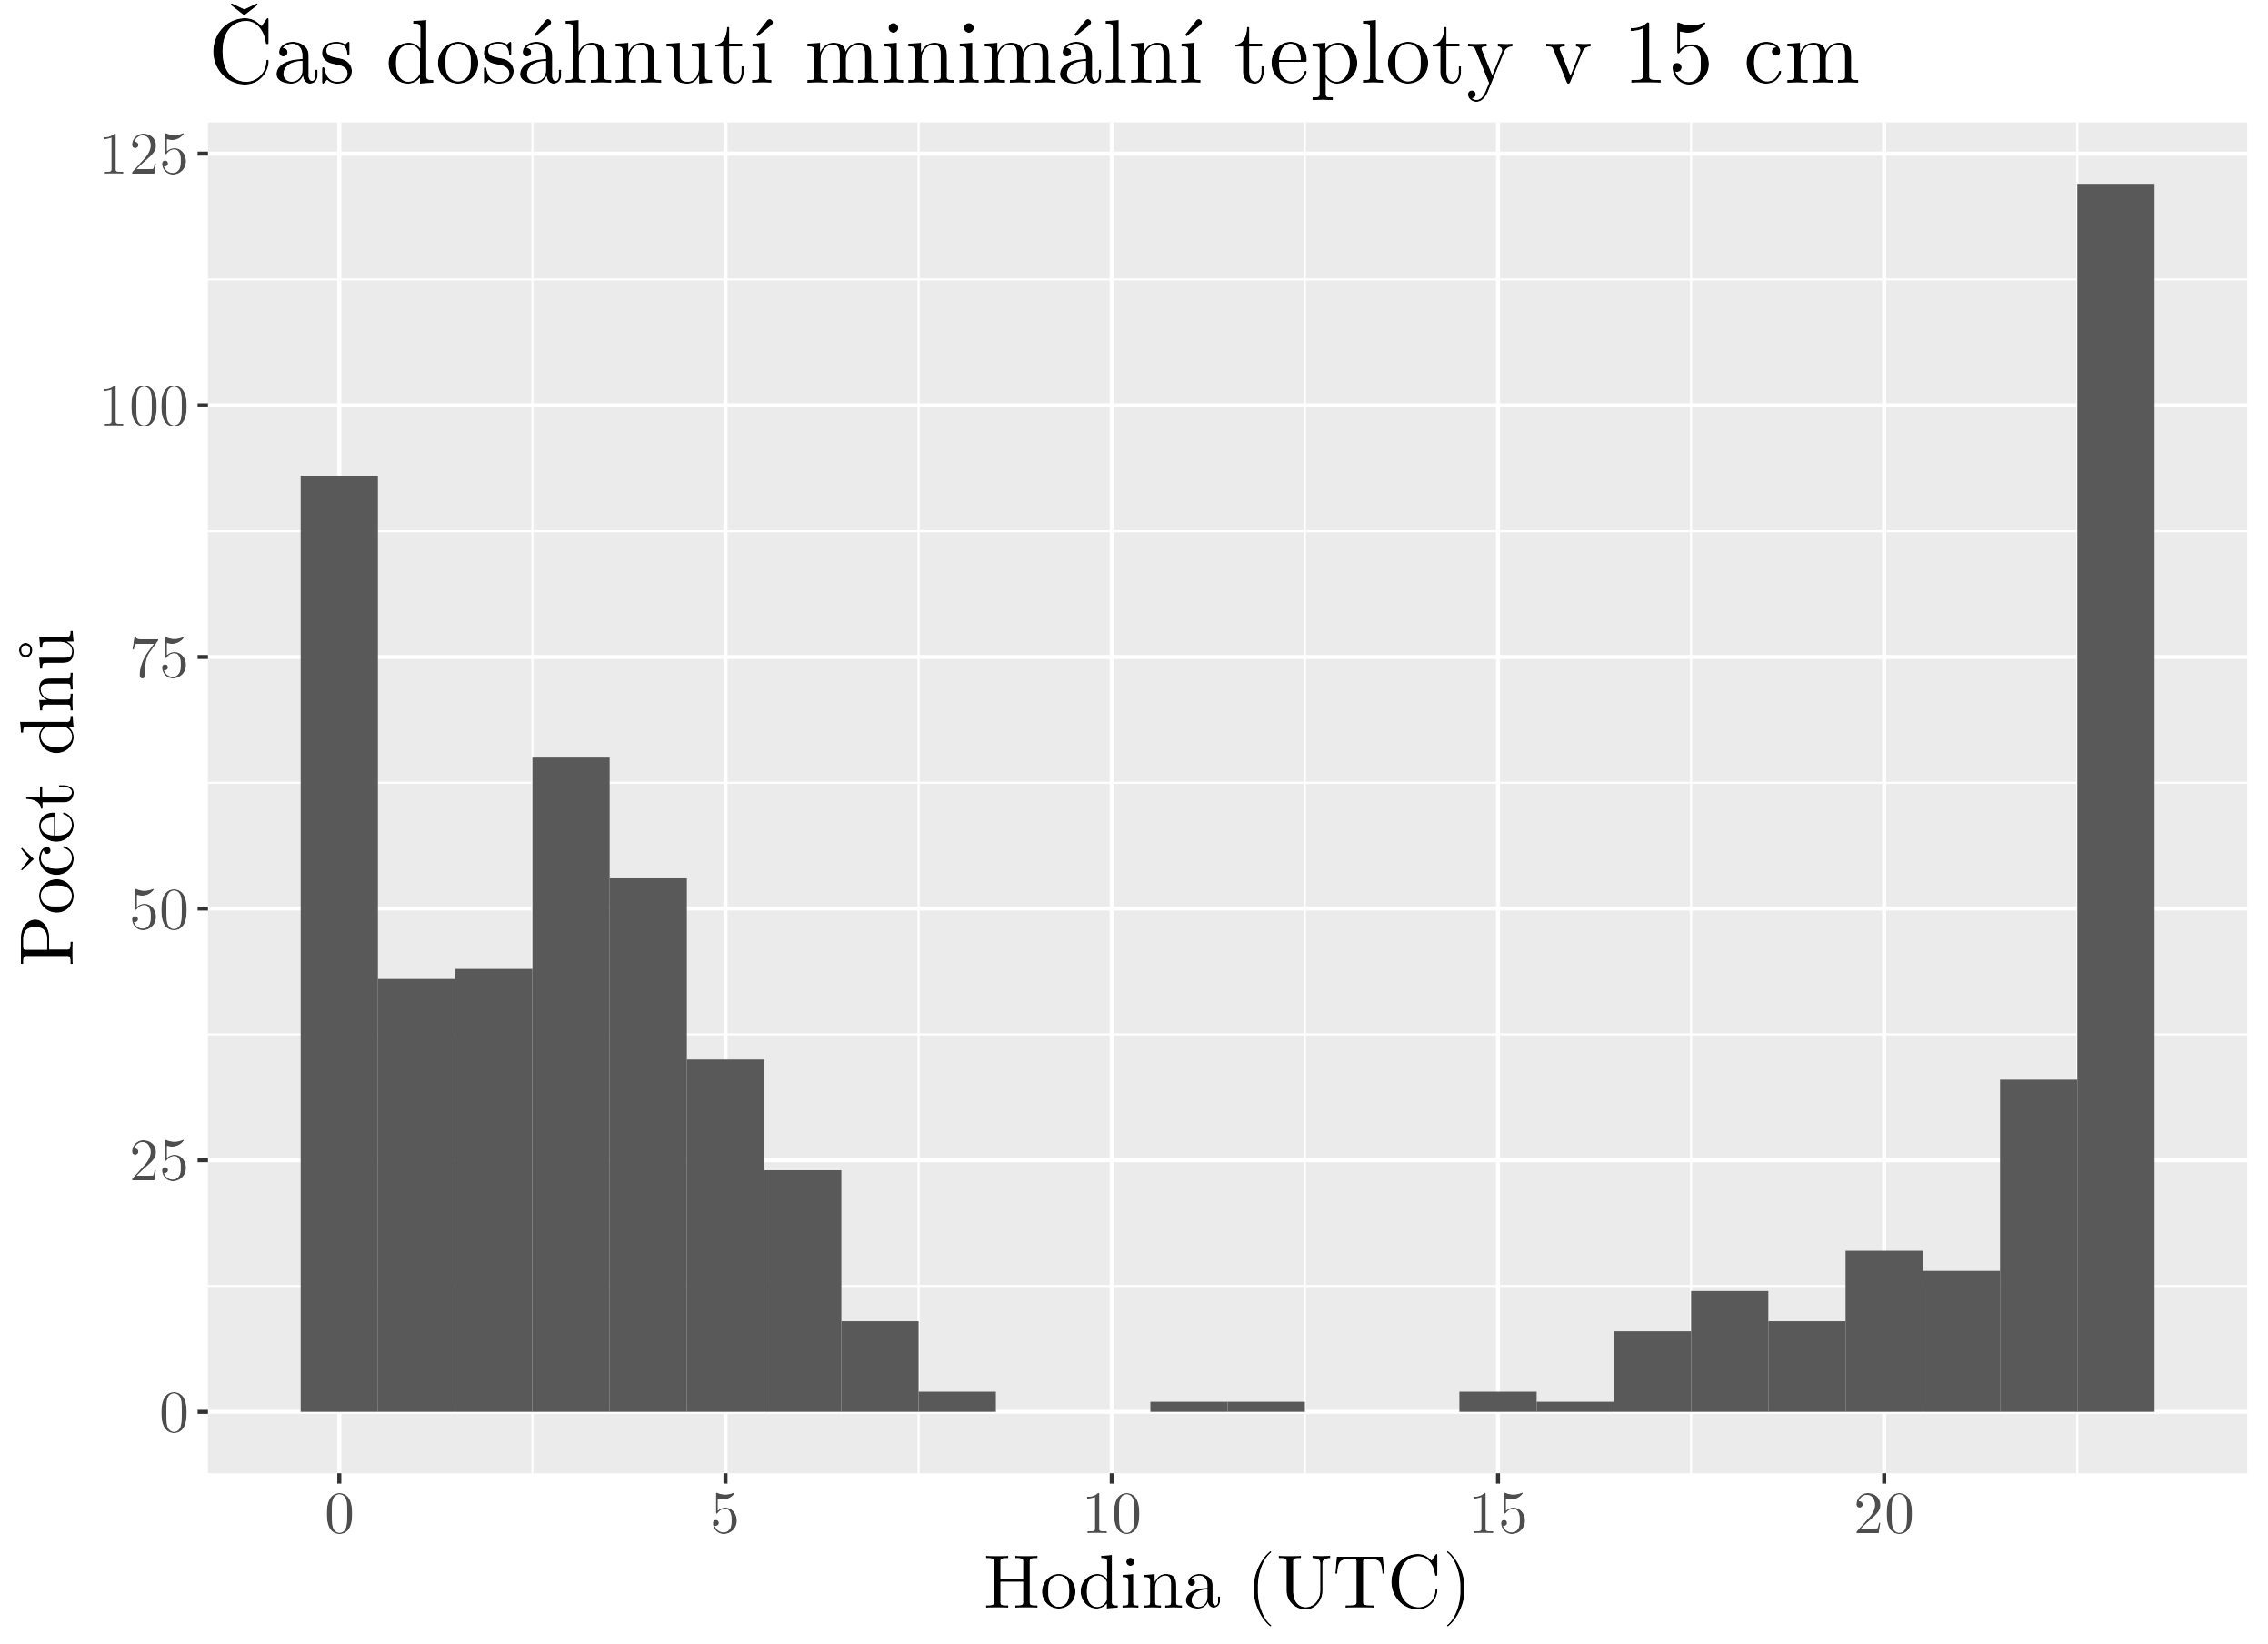
\includegraphics[width=\textwidth]{img/hist_hourmin15cm.png}
		\caption{}
		\label{fig:hourmin15cm}
	\end{subfigure}
	\hfill
	\begin{subfigure}{0.45\textwidth}
  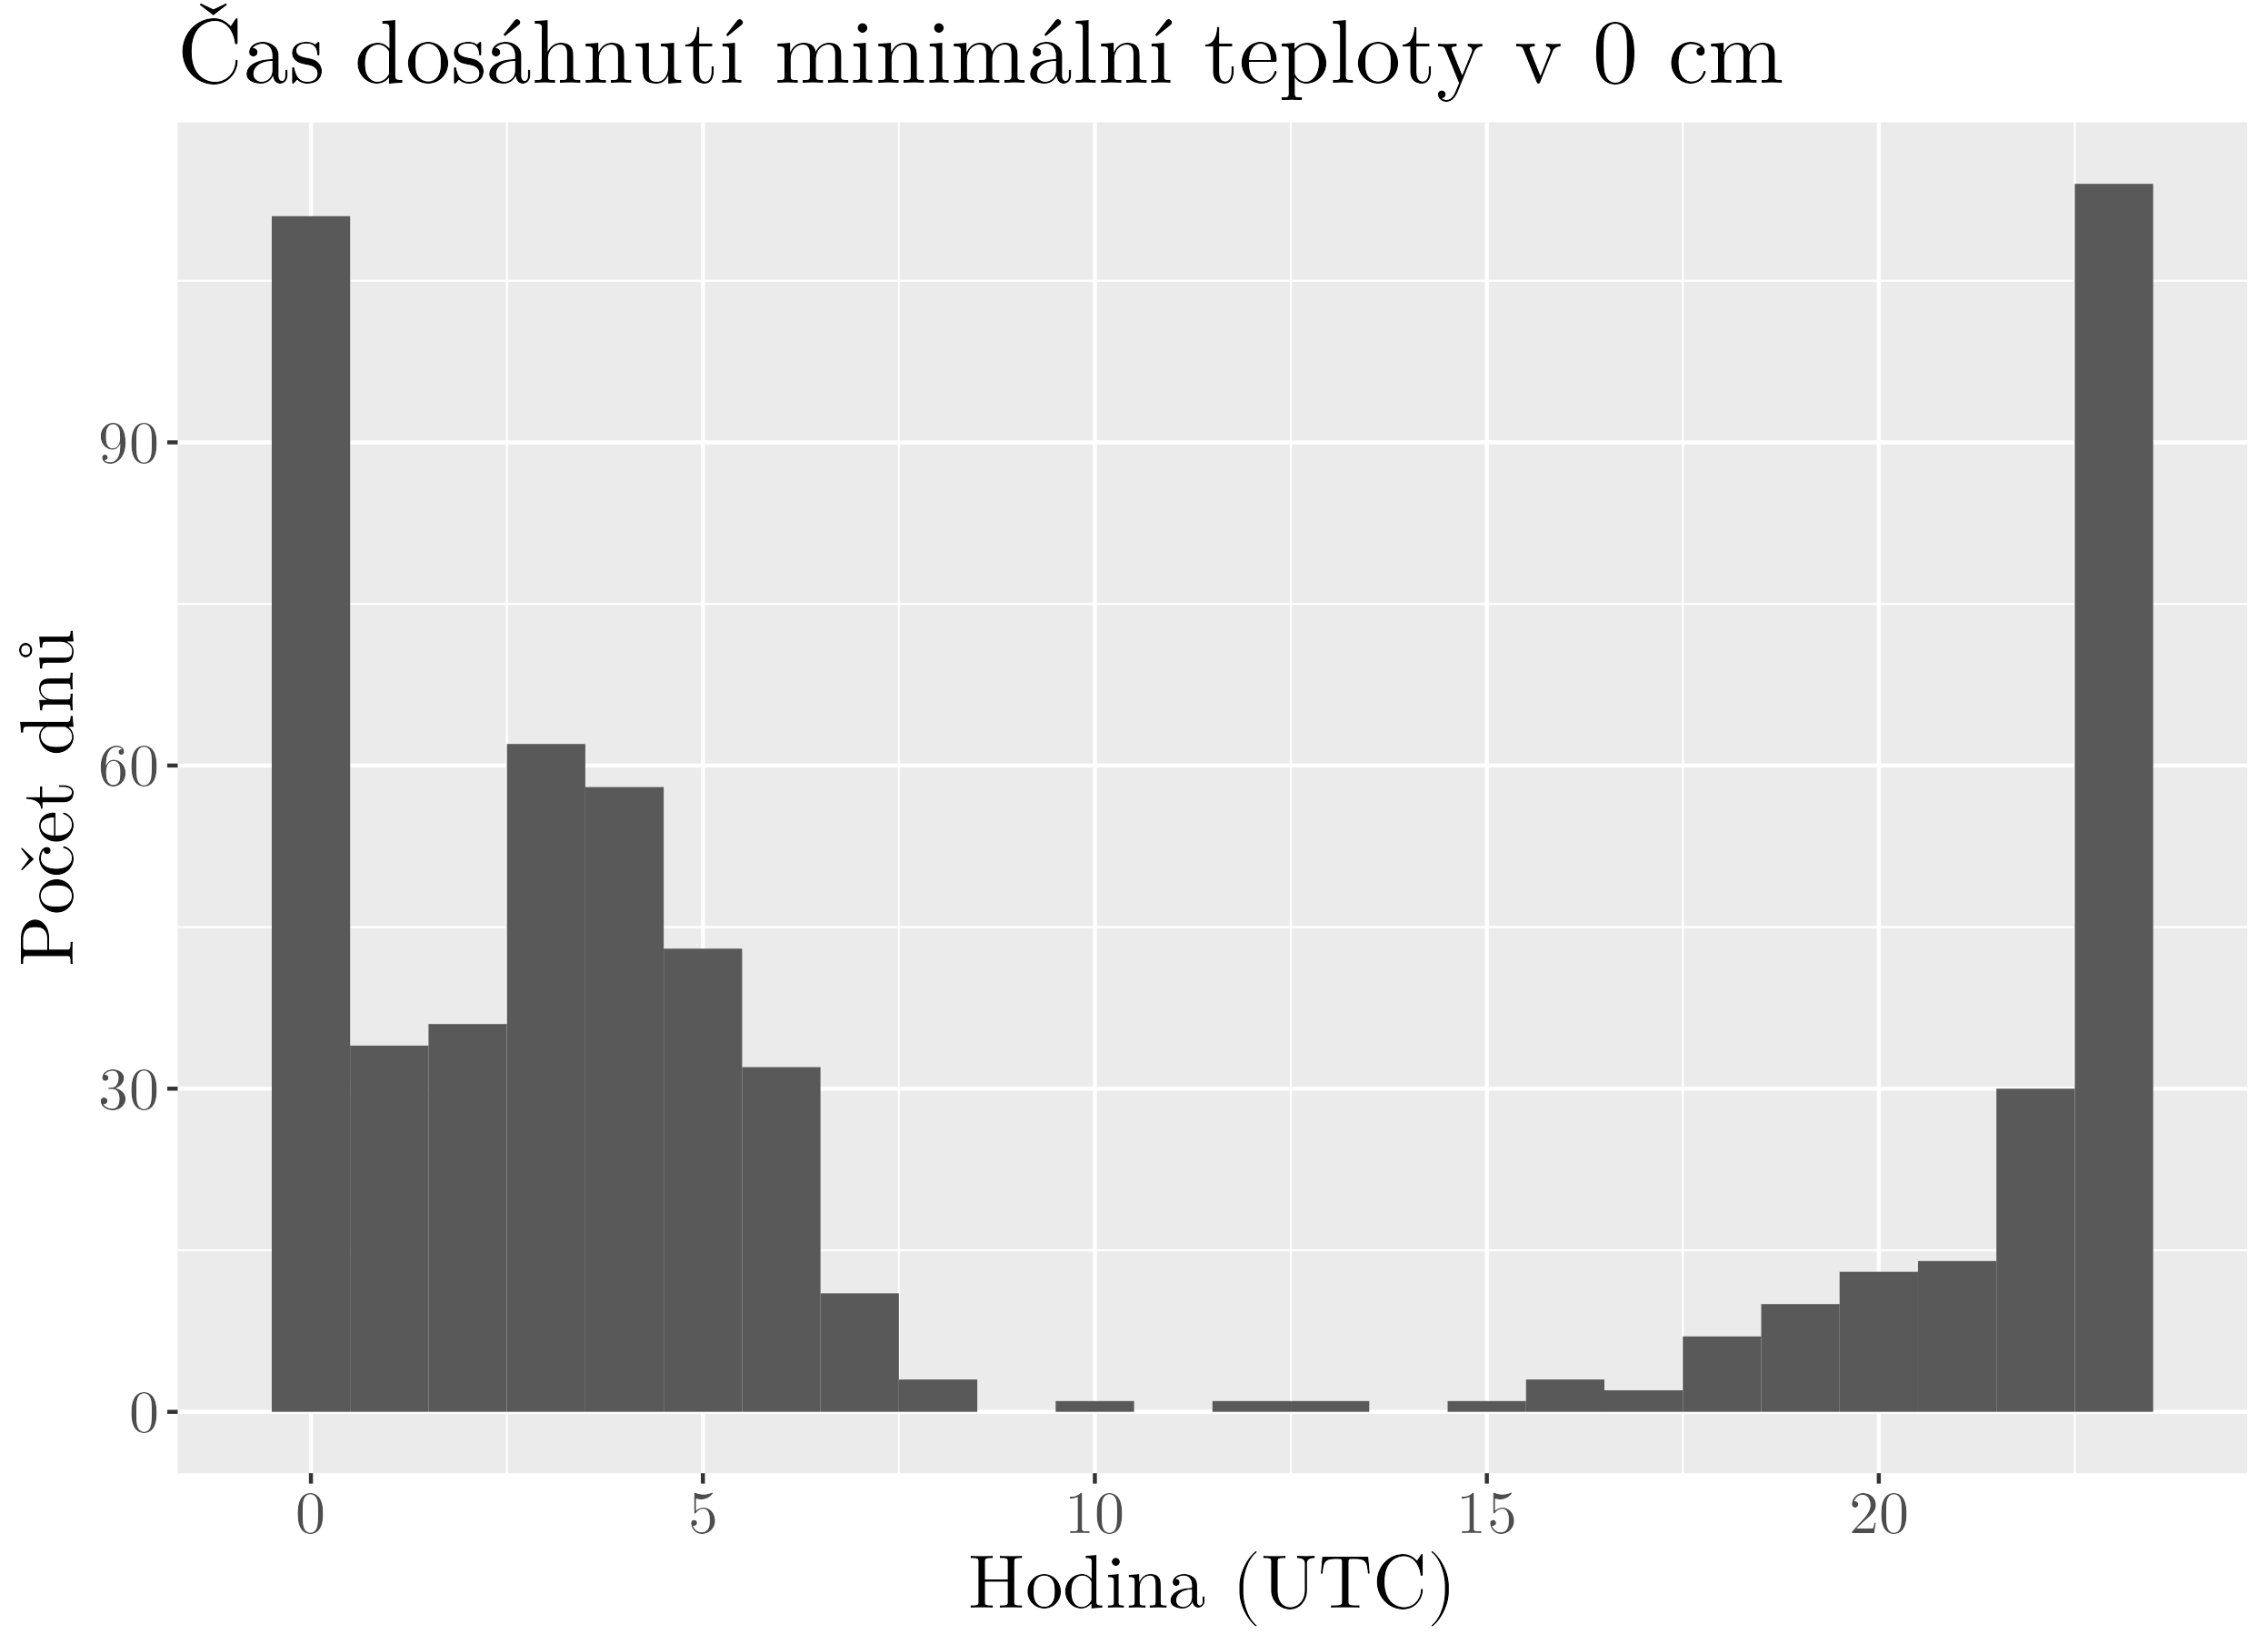
\includegraphics[width=\textwidth]{img/hist_hourmin0cm.png}
		\caption{}
		\label{fig:hourmin0cm}
	\end{subfigure}
	\caption{Denní doba (UTC) dosažení maximální resp. minimální teploty v $\SI{15}{cm}$ resp. v $\SI{0}{cm}$ nad zemí na čidle nejblíže stanici Churáňov}
	\label{fig:hours}
\end{figure}

Pro ilustraci se podívejme na konkrétní hodnoty teplot pozorované na nejbližším čidlu meteorologické stanice Churáňov. Na obrázcích \ref{fig:maxtemp} můžeme vidět průběh denních minim a maxim na jednom z čidel, celkově jde o 587 dní, období od 12.10.2019 do 20.5.2021. Na obrázcích \ref{fig:2mhours} můžeme vidět hodnoty teplot naměřených ve výšce $\SI{2}{m}$ na čidle zavěšeném na stromě poblíž pozemním čidlům, jde o hodnoty naměřené v době denního teplotního maxima a minima ve výšce $\SI{15}{cm}$.

\begin{figure}
	\centering
	\begin{subfigure}{0.45\textwidth}
  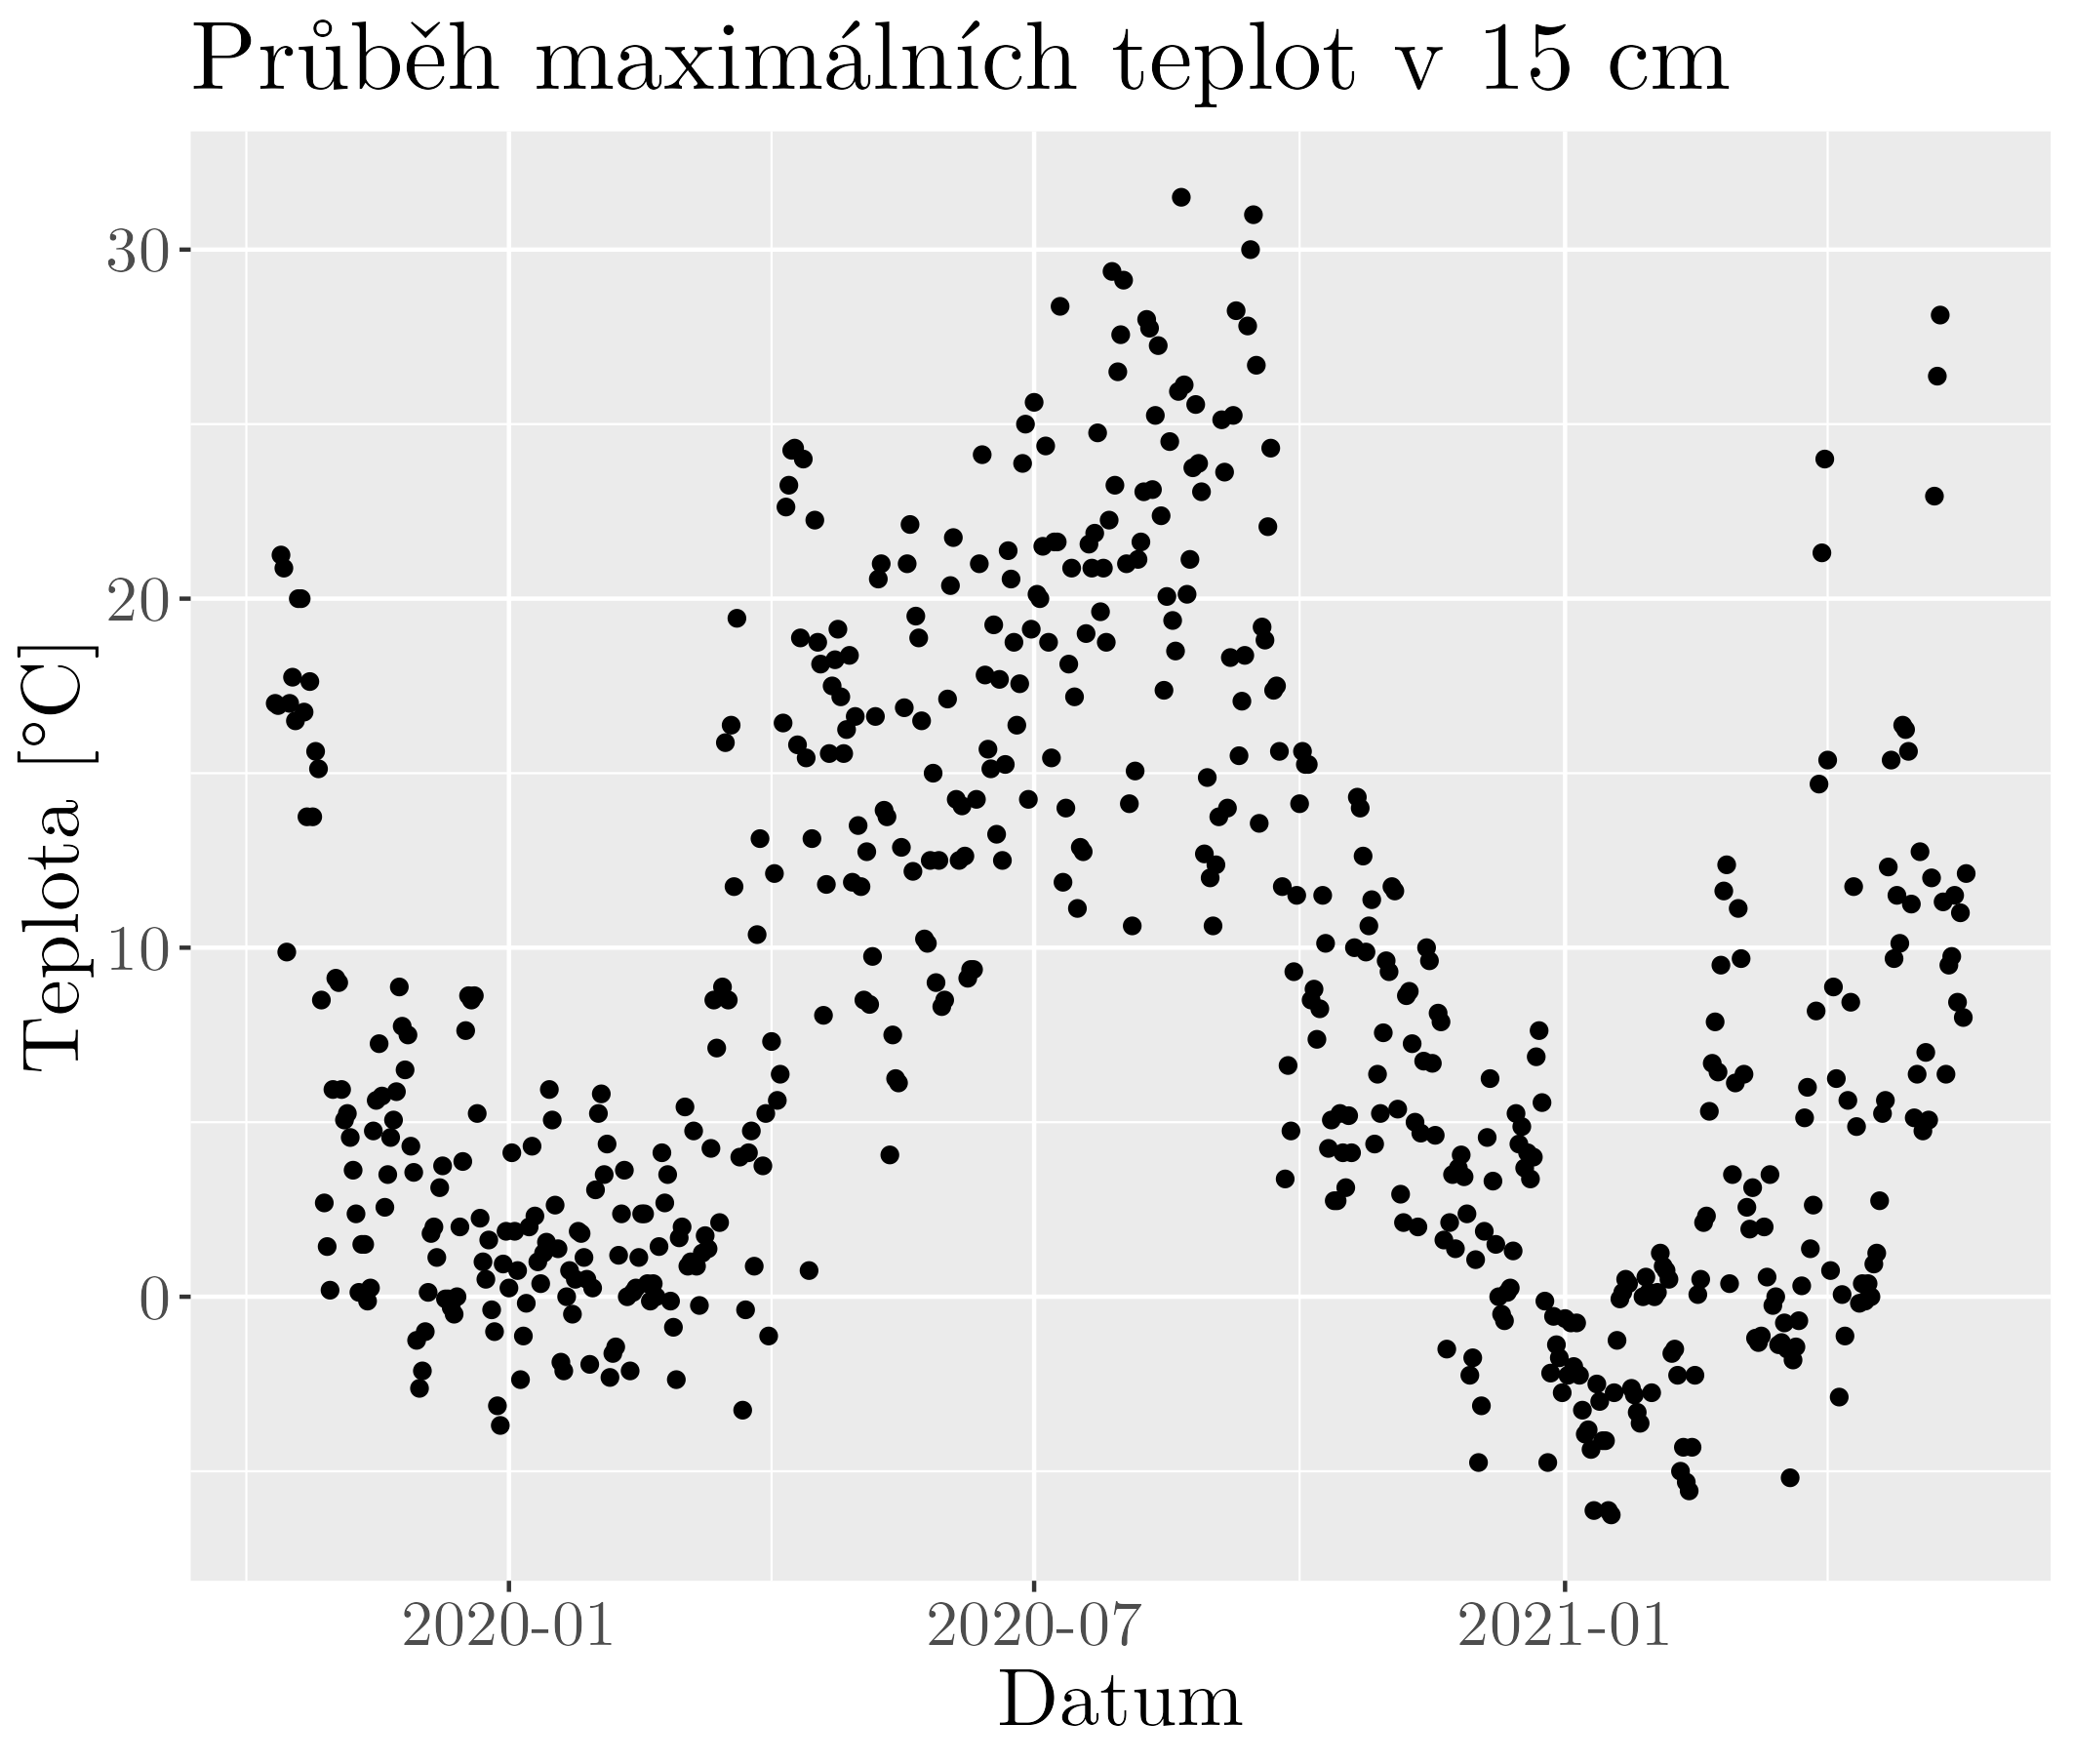
\includegraphics[width=\textwidth]{img/maxtempmax15cm.png}
		\caption{}
		\label{fig:maxtempmax15cm}
	\end{subfigure}
	\hfill
	\begin{subfigure}{0.45\textwidth}
  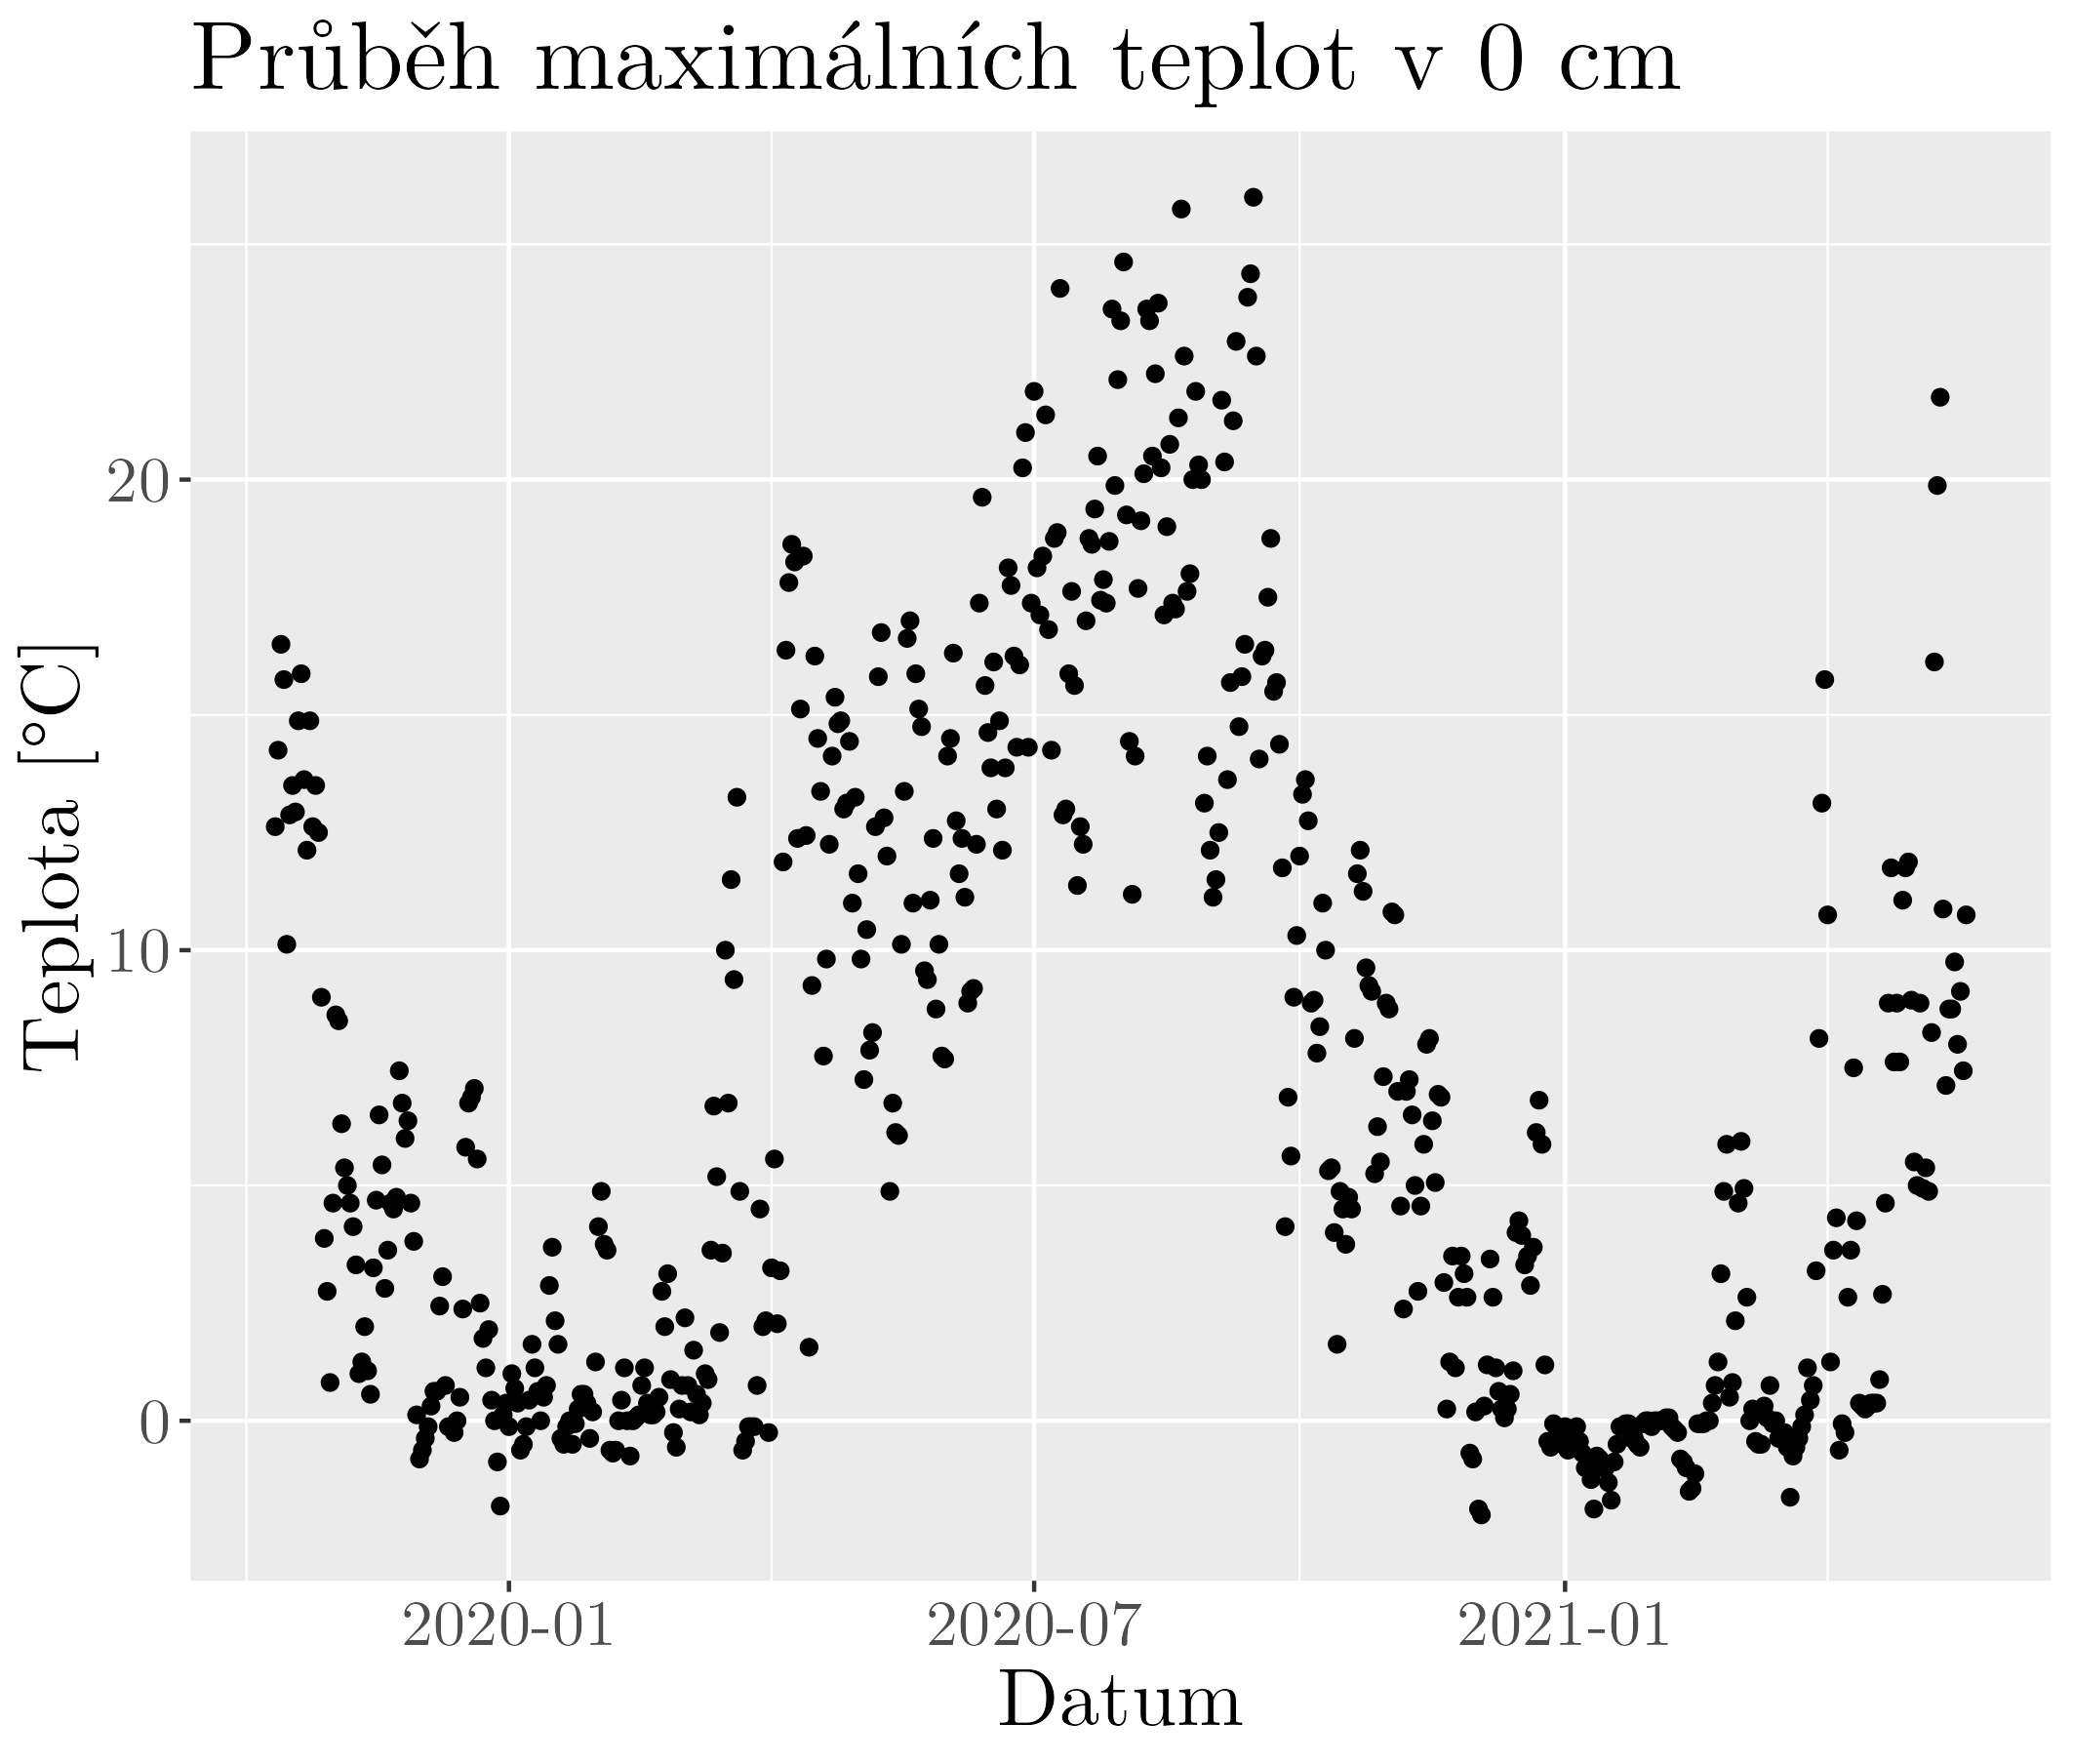
\includegraphics[width=\textwidth]{img/maxtempmax0cm.png}
		\caption{}
		\label{fig:maxtempmax0cm}
	\end{subfigure}
	\hfill
	\begin{subfigure}{0.45\textwidth}
  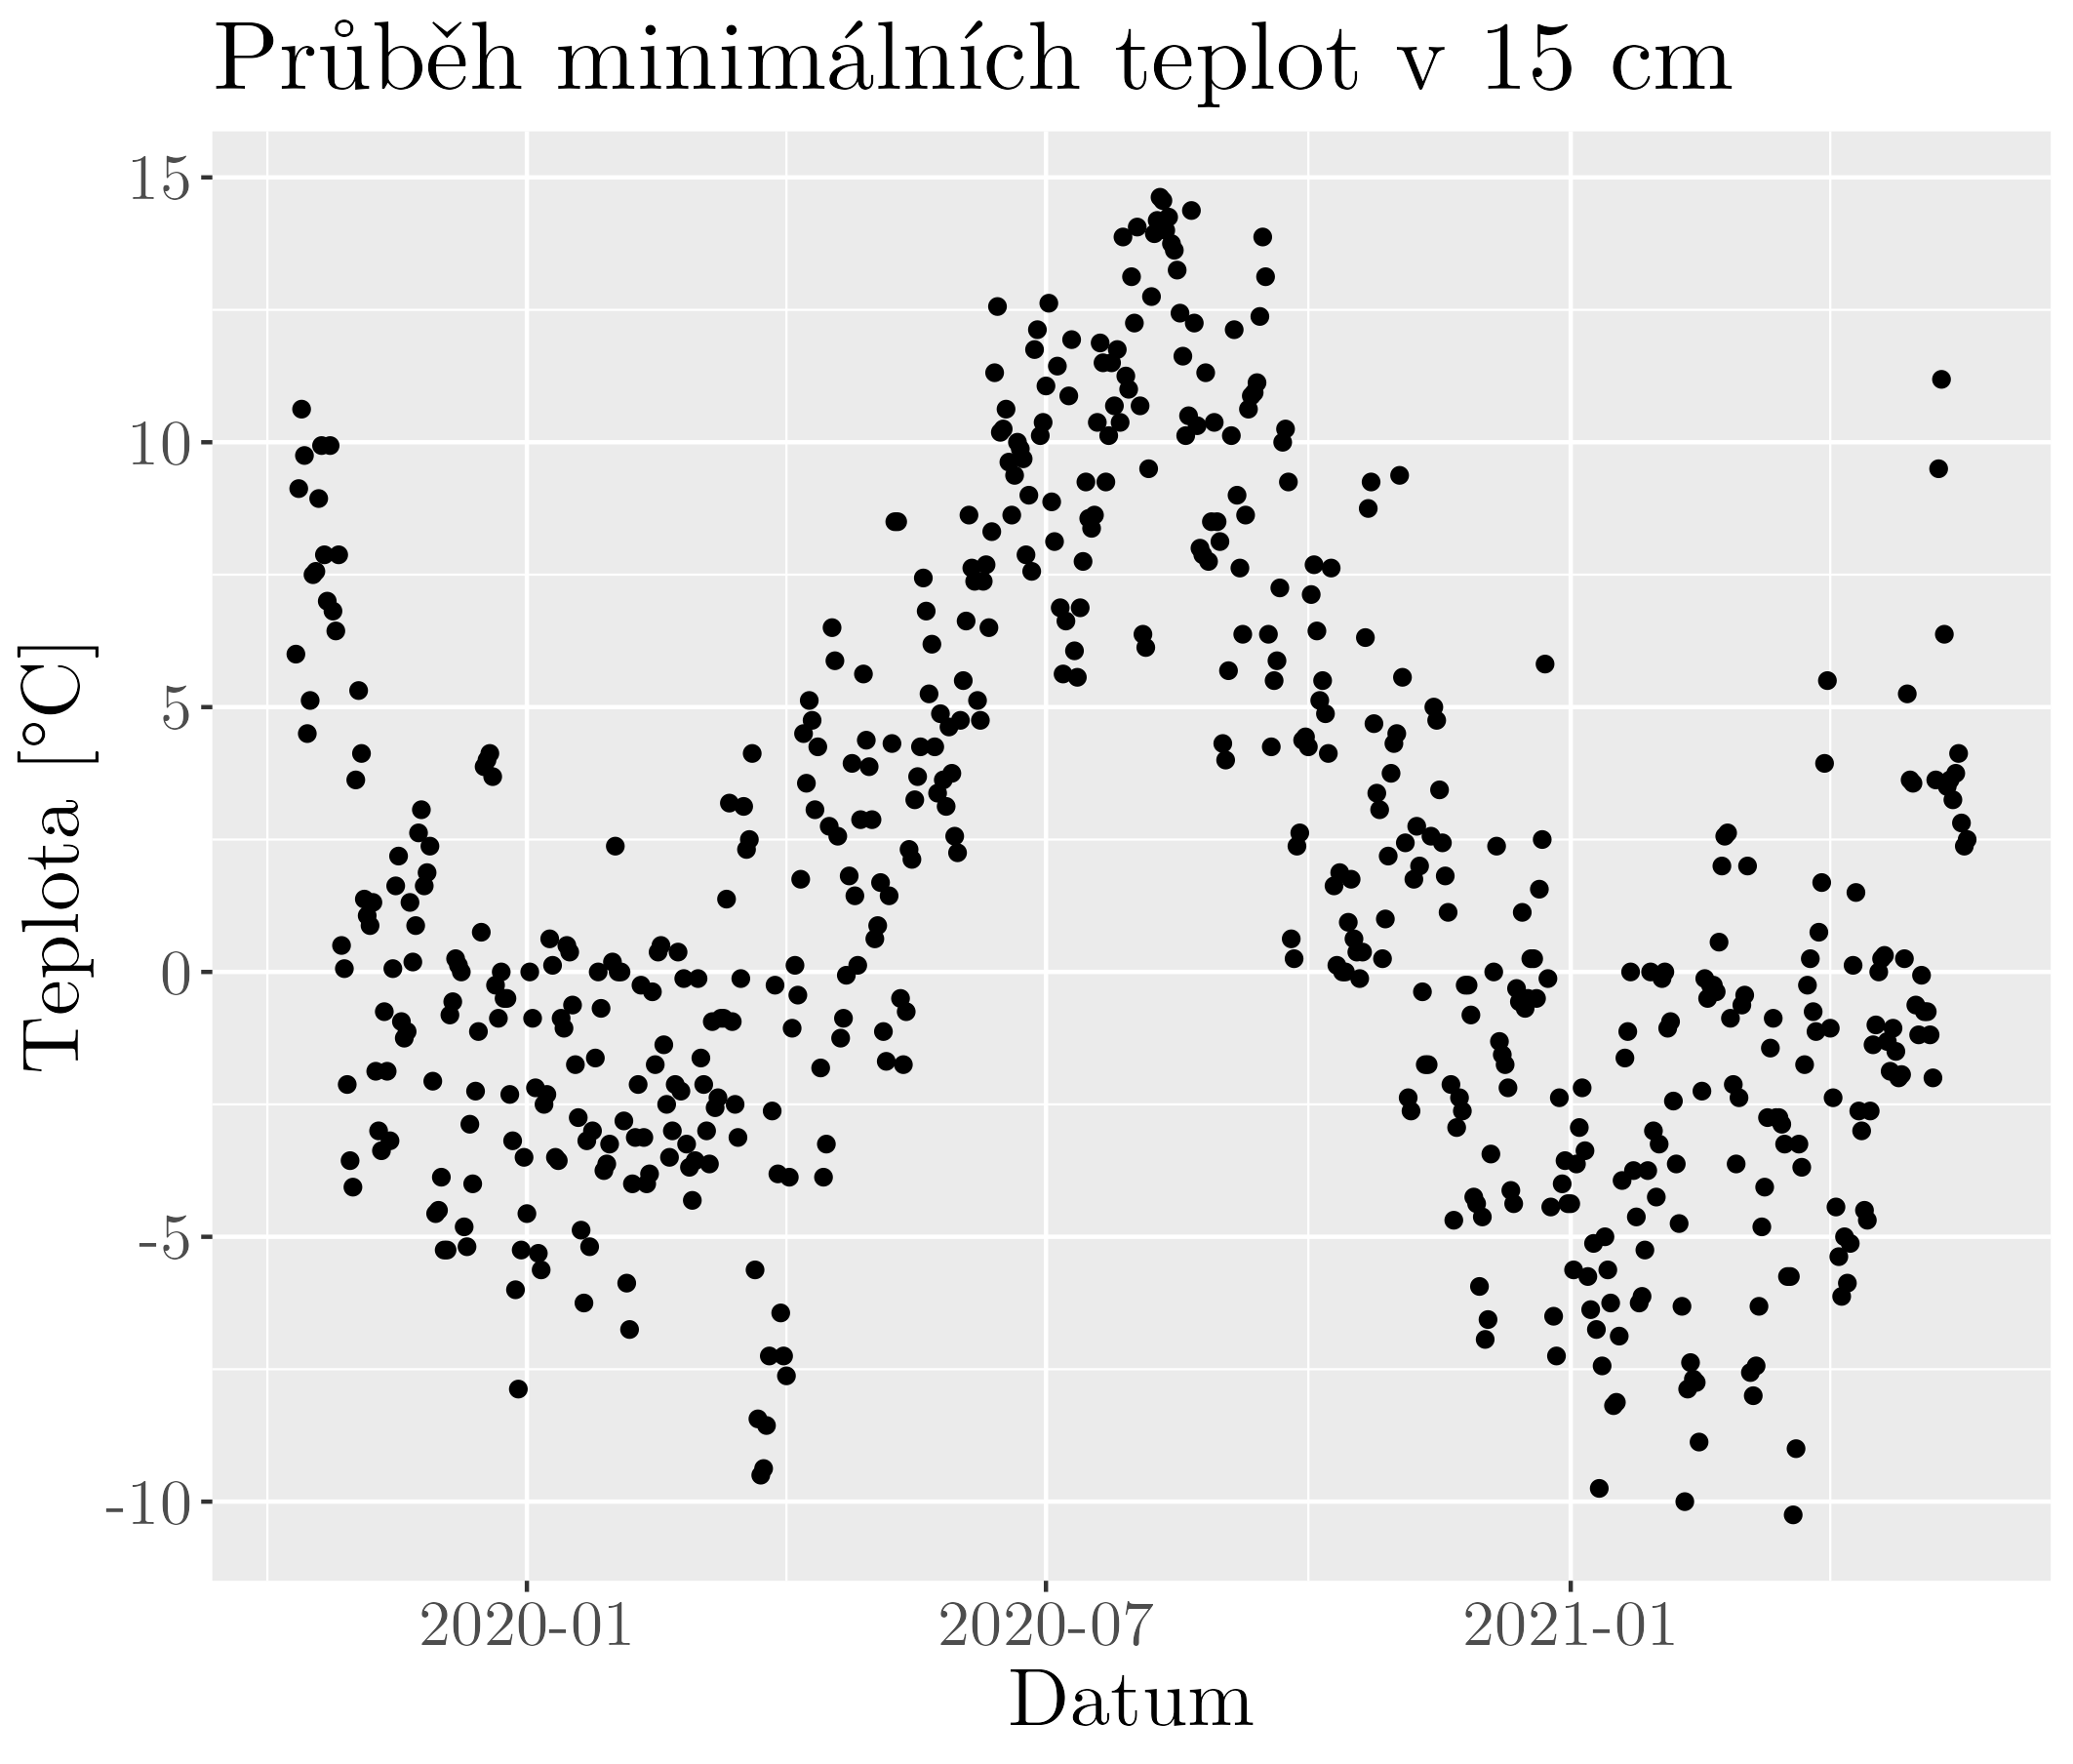
\includegraphics[width=\textwidth]{img/maxtempmin15cm.png}
		\caption{}
		\label{fig:maxtempmin15cm}
	\end{subfigure}
	\hfill
	\begin{subfigure}{0.45\textwidth}
  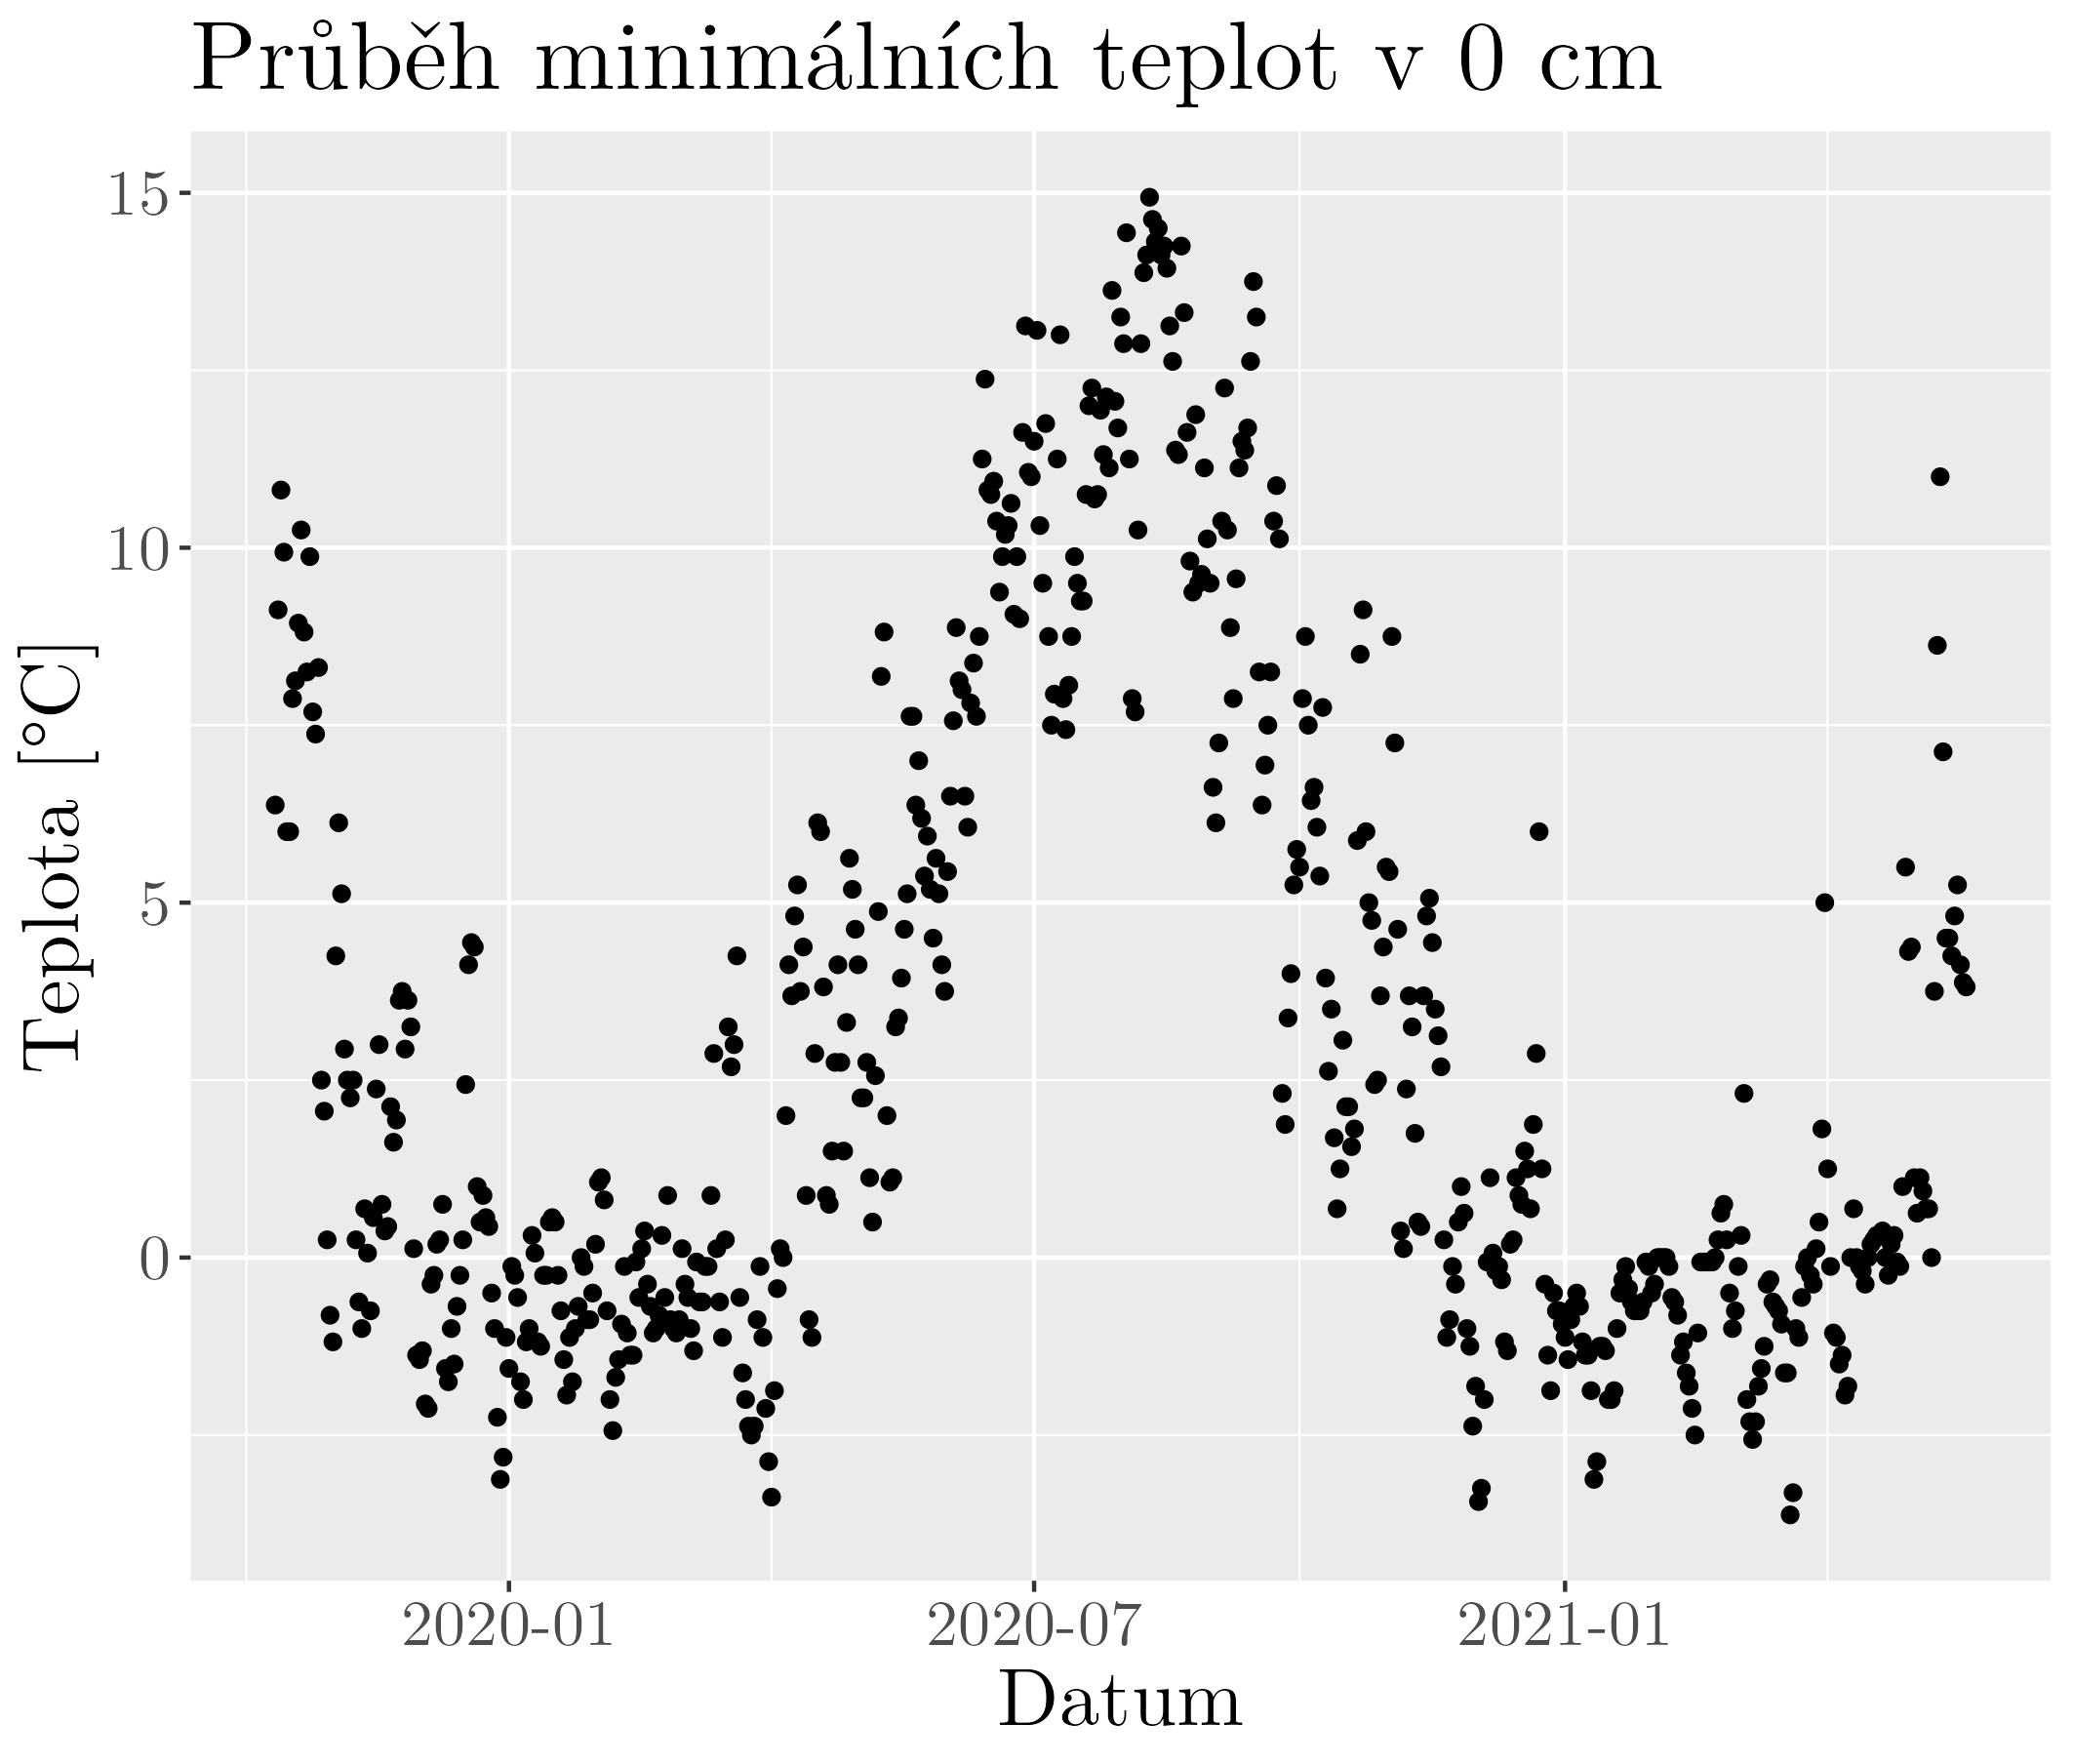
\includegraphics[width=\textwidth]{img/maxtempmin0cm.png}
		\caption{}
		\label{fig:maxtempmin0cm}
	\end{subfigure}
	\caption{Průběh denních maximální resp. minimálních teplot ve výšce $\SI{15}{cm}$ resp. $\SI{0}{cm}$ nad zemí na čidle nejblíže stanici Churáňov}
	\label{fig:maxtemp}
\end{figure}

\begin{figure}
	\centering
	\begin{subfigure}{0.45\textwidth}
  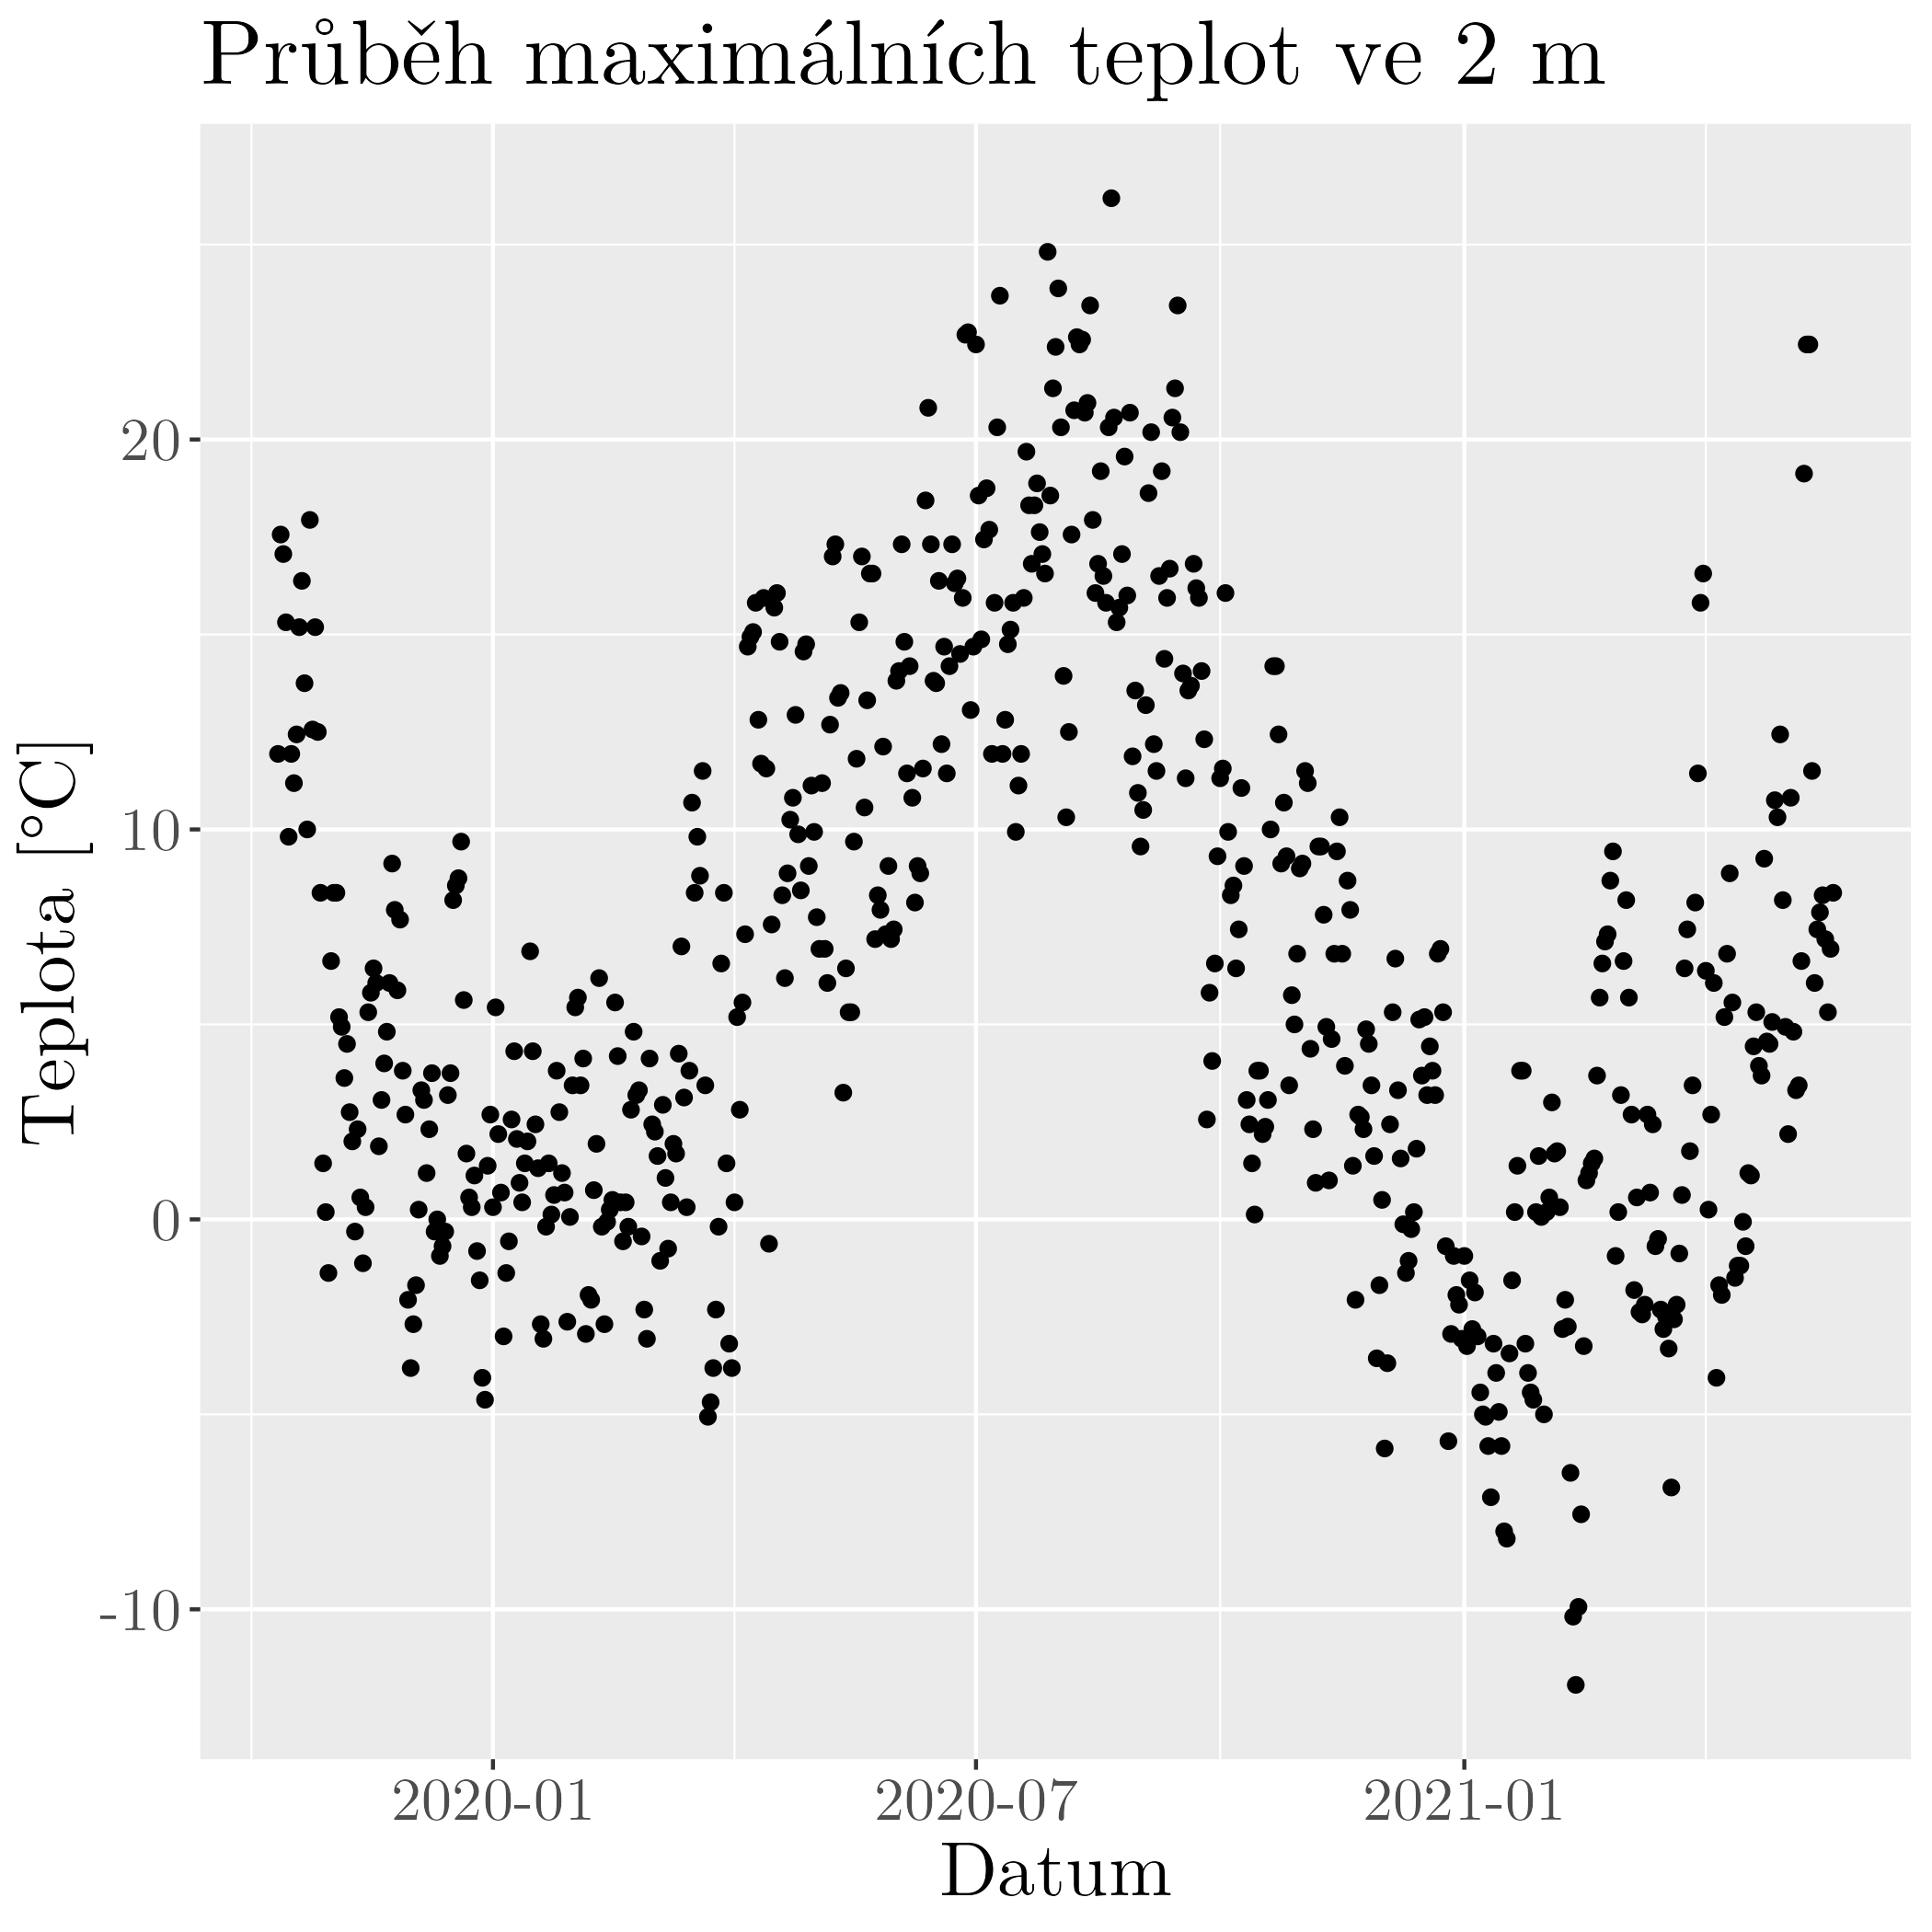
\includegraphics[width=\textwidth]{img/2mmaxtempmax15cm.png}
		\caption{Teploty naměřené ve stejnou dobu jako maximální teploty v $\SI{15}{cm}$}
		\label{fig:2mmaxtempmax15cm}
	\end{subfigure}
	\hfill
	\begin{subfigure}{0.45\textwidth}
  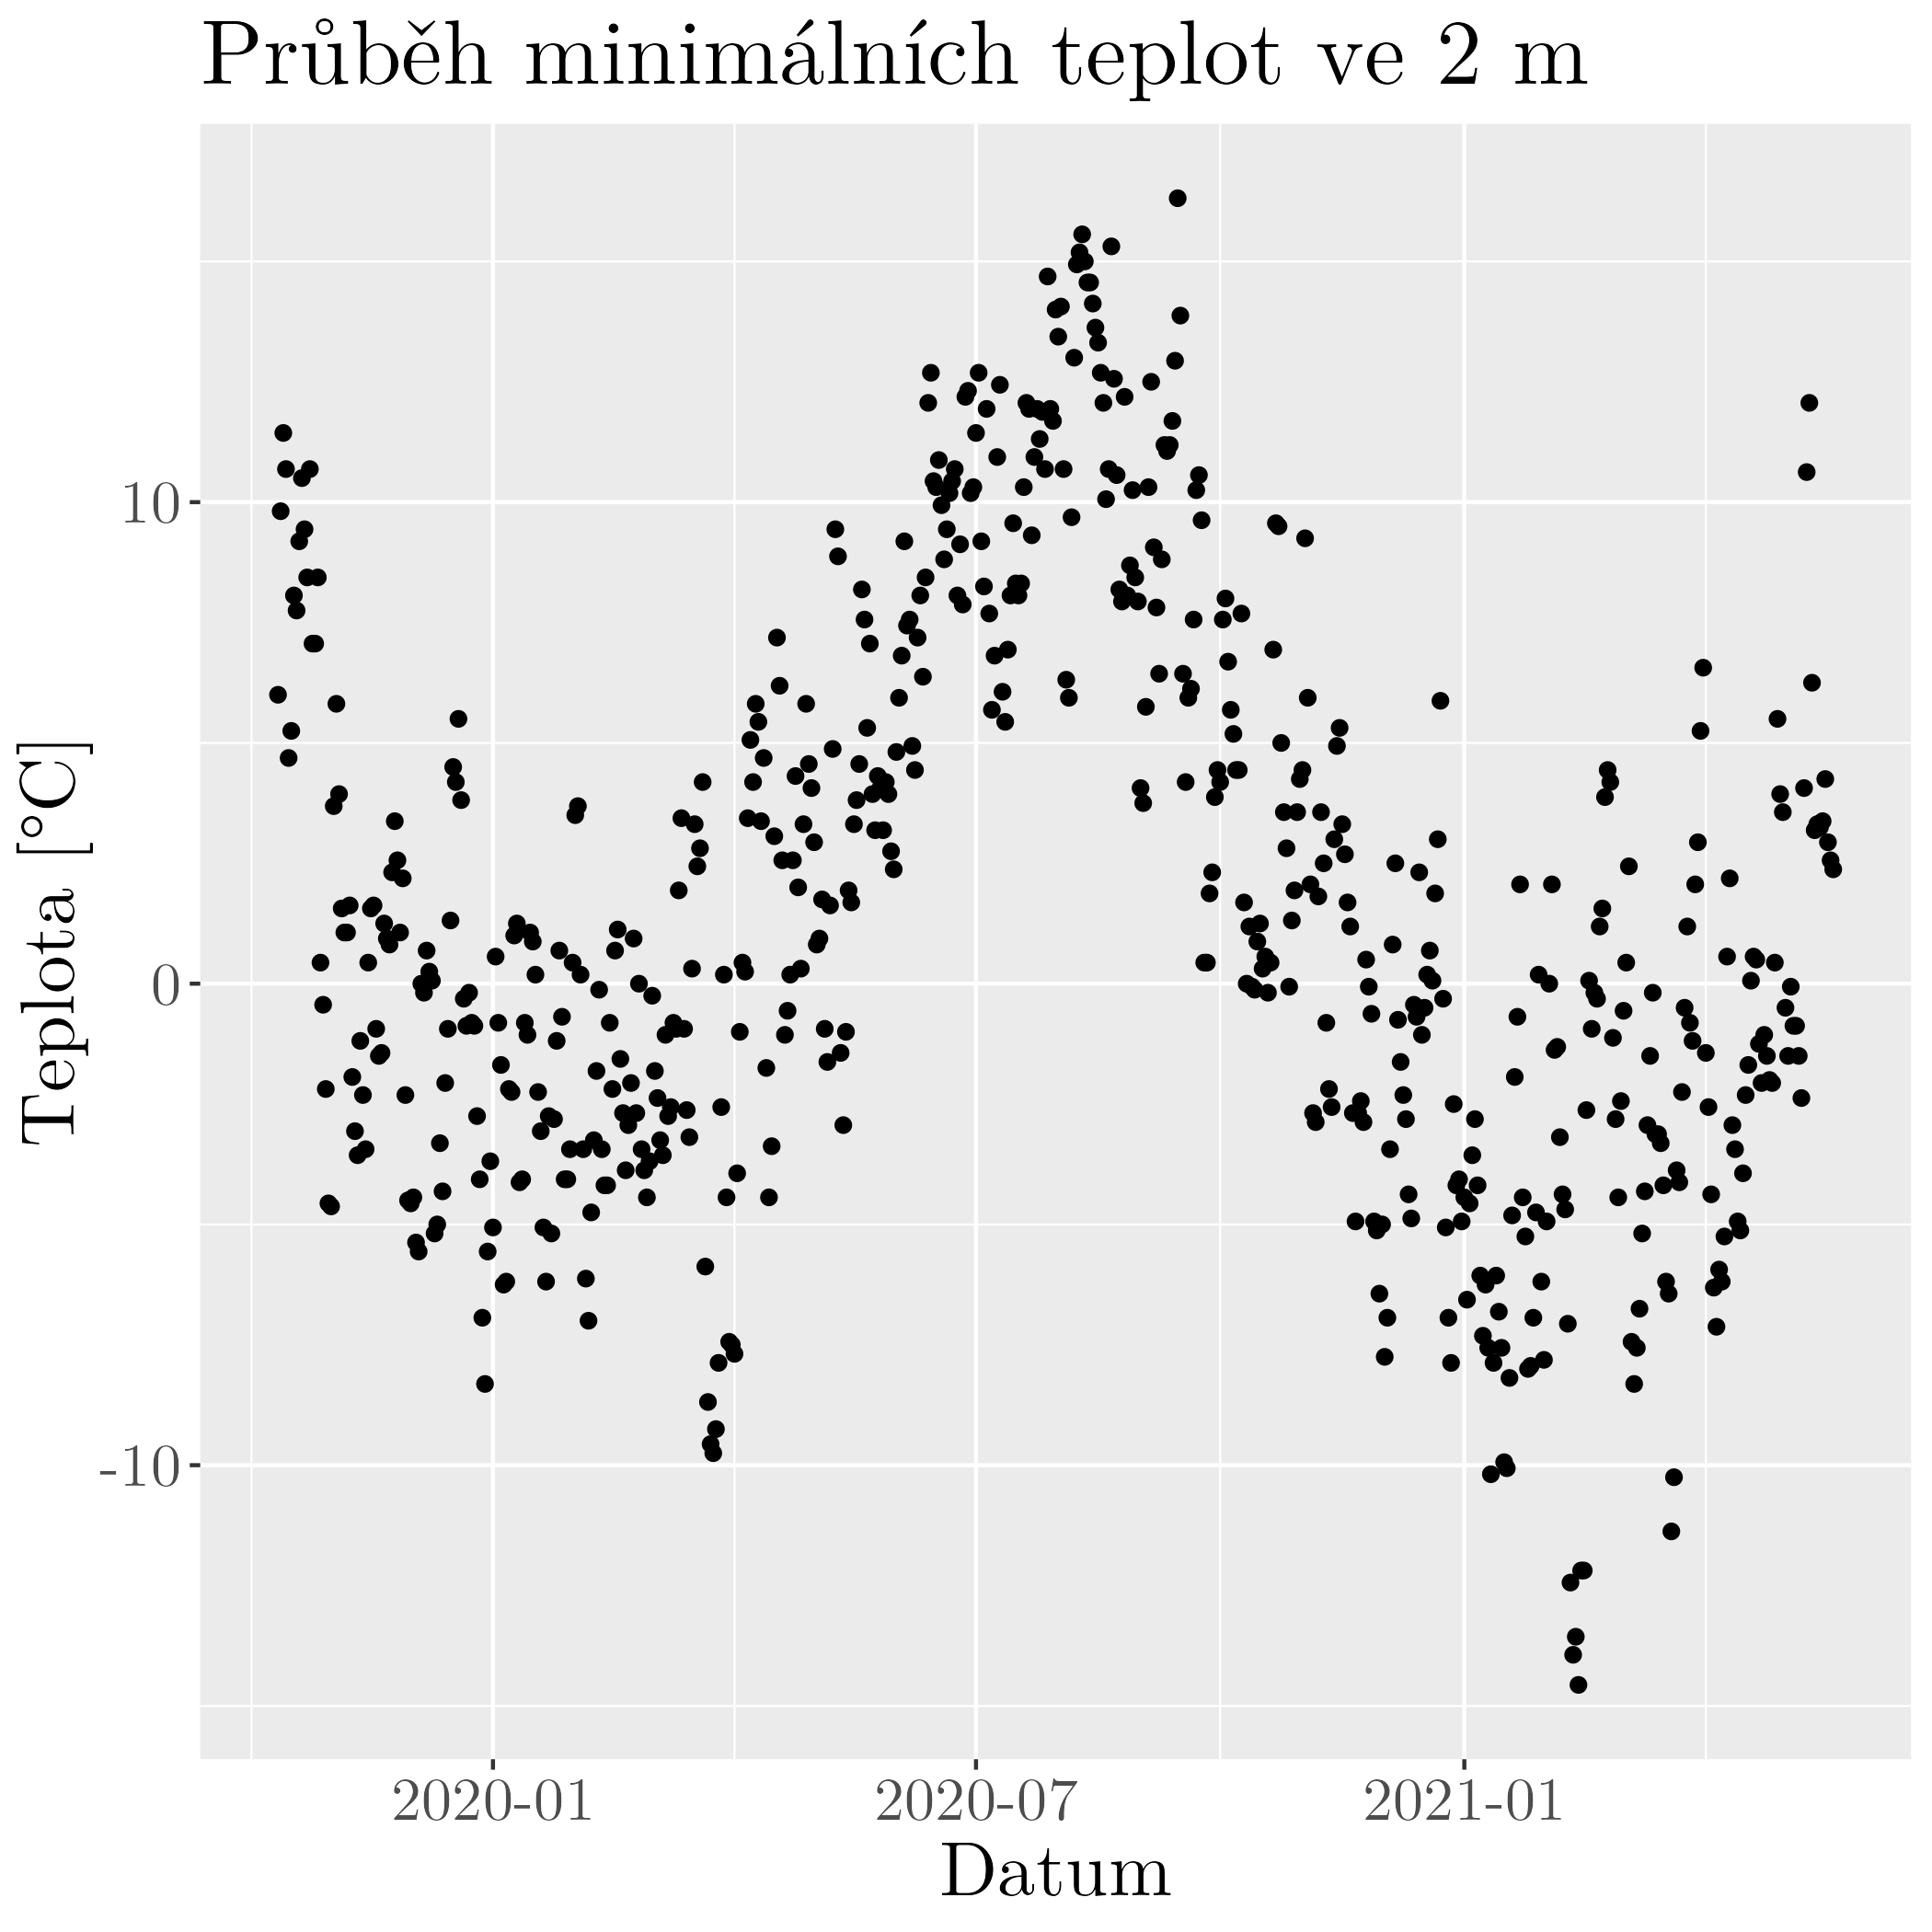
\includegraphics[width=\textwidth]{img/2mmaxtempmin15cm.png}
		\caption{Teploty naměřené ve stejnou dobu jako minimální teploty v $\SI{15}{cm}$}
		\label{fig:2mmaxtempmin15cm}
	\end{subfigure}
	\caption{Teploty ve výšce $\SI{2}{m}$ nad zemí na čidle nejblíže stanici Churáňov v době kdy nastalo maximum resp. minimum na čidle ve výšce $\SI{15}{cm}$}
	\label{fig:2mhours}
\end{figure}

Na obrázku \ref{fig:hist_diff} můžeme vidět histogramy rozdílů teplot pro jednotlivé výšky a pro maxima a minima.

\begin{figure}
	\centering
	\begin{subfigure}{0.45\textwidth}
  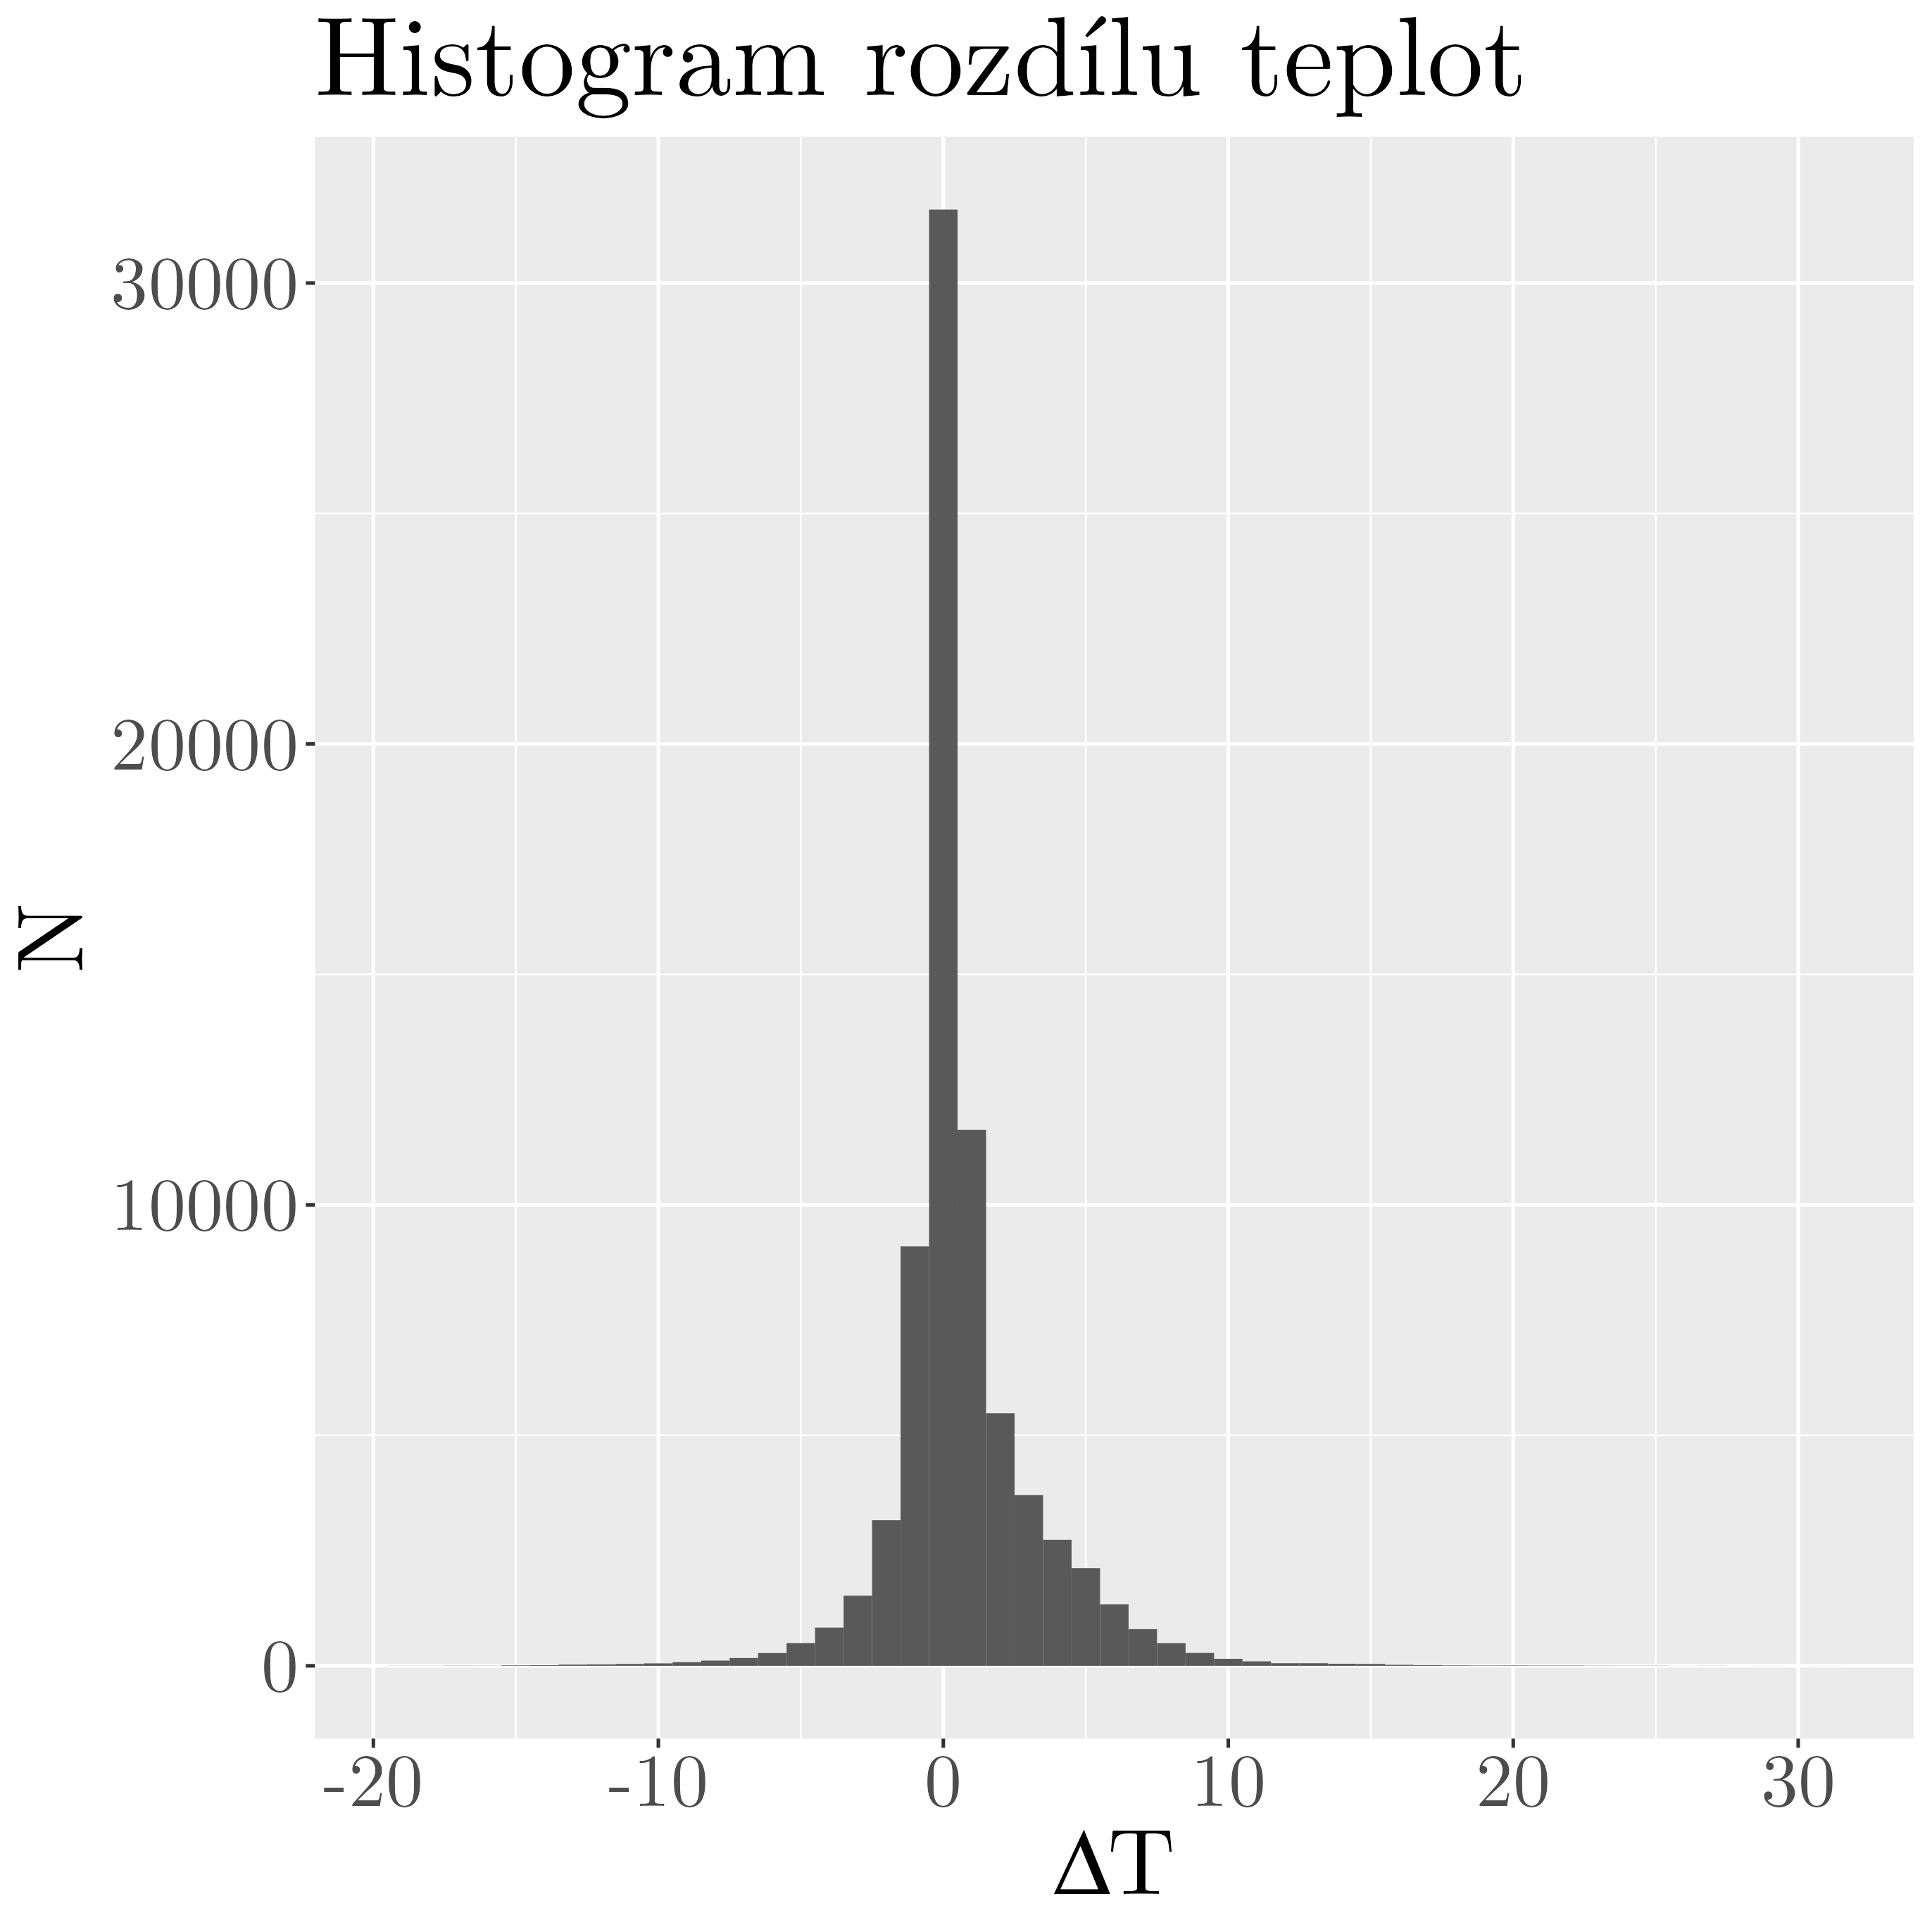
\includegraphics[width=\textwidth]{img/ch2/hist_diff_max15cm.png}
		\caption{Histogram rozdílu maximálních teplot v $\SI{15}{cm}$ a $\SI{2}{m}$. $\text{M} = 0.69$, $\text{MD} = 0.25$.}
		\label{fig:hist_diff_max15cm}
	\end{subfigure}
	\hfill
	\begin{subfigure}{0.45\textwidth}
  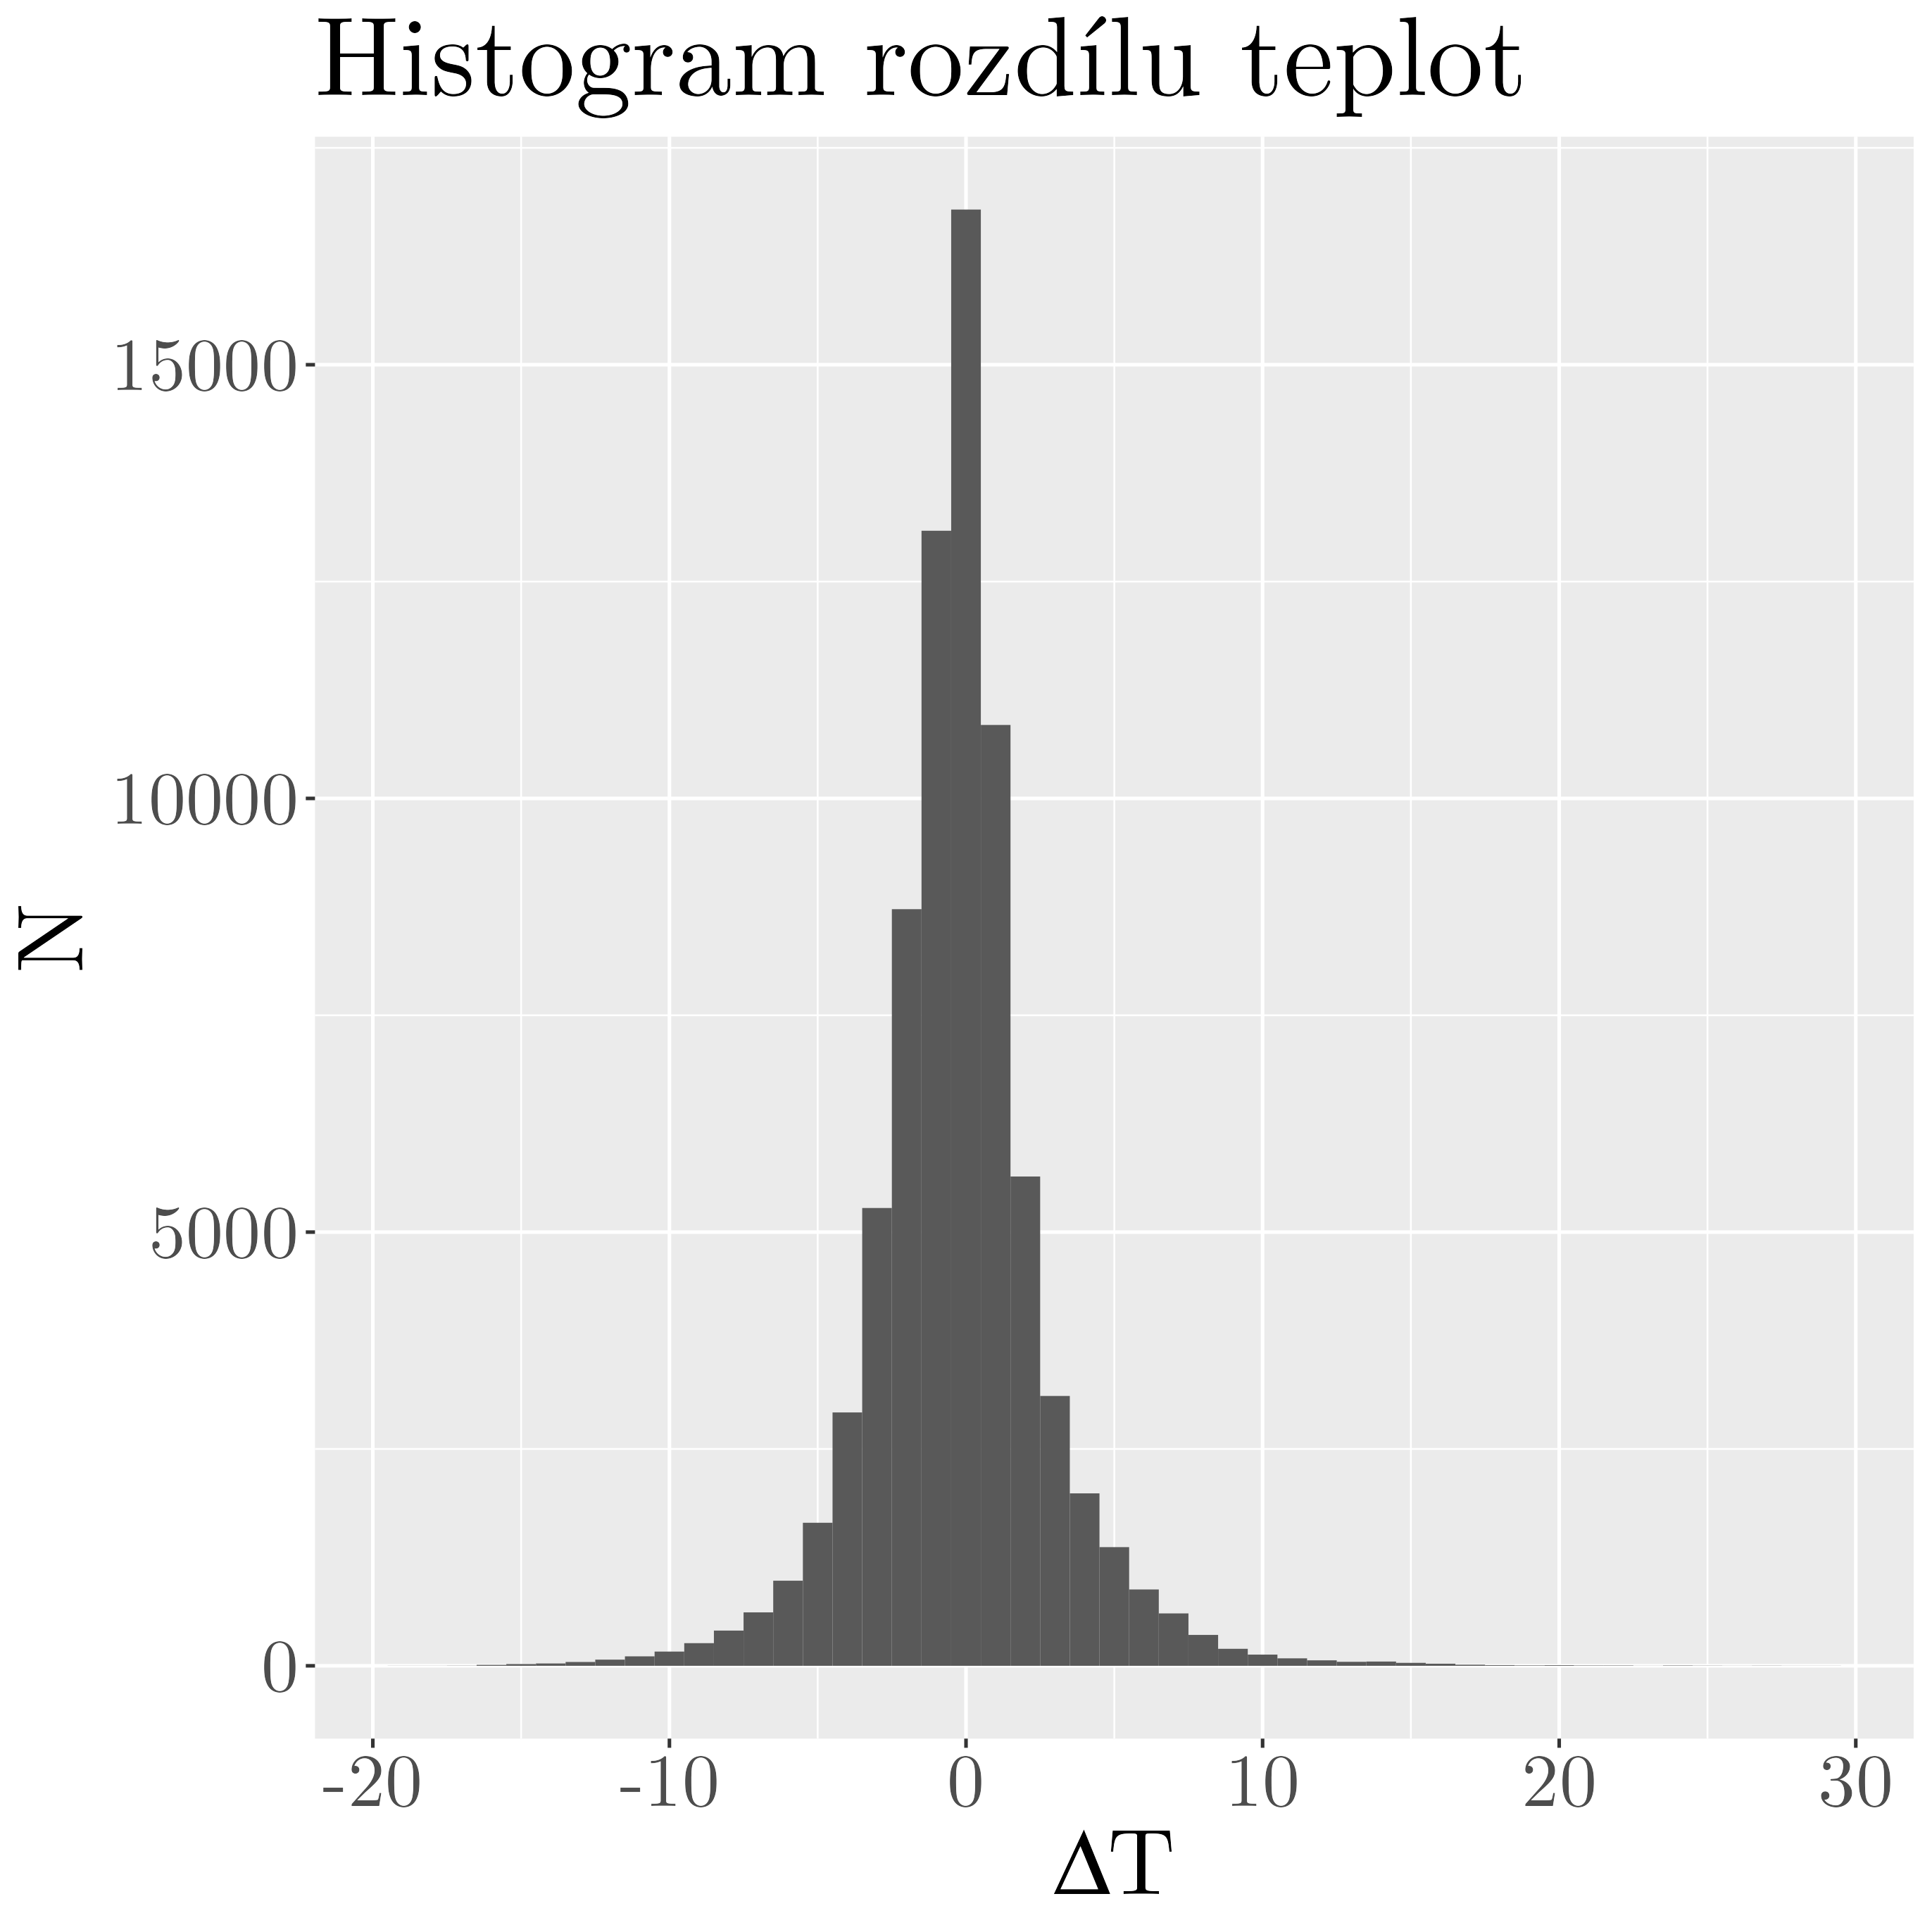
\includegraphics[width=\textwidth]{img/ch2/hist_diff_max0cm.png}
		\caption{Histogram rozdílu maximálních teplot v $\SI{0}{cm}$ a $\SI{2}{m}$. $\text{M} = -0.24$, $\text{MD} = -0.25$.}
		\label{fig:hist_diff_max0cm}
	\end{subfigure}
	\hfill
	\begin{subfigure}{0.45\textwidth}
  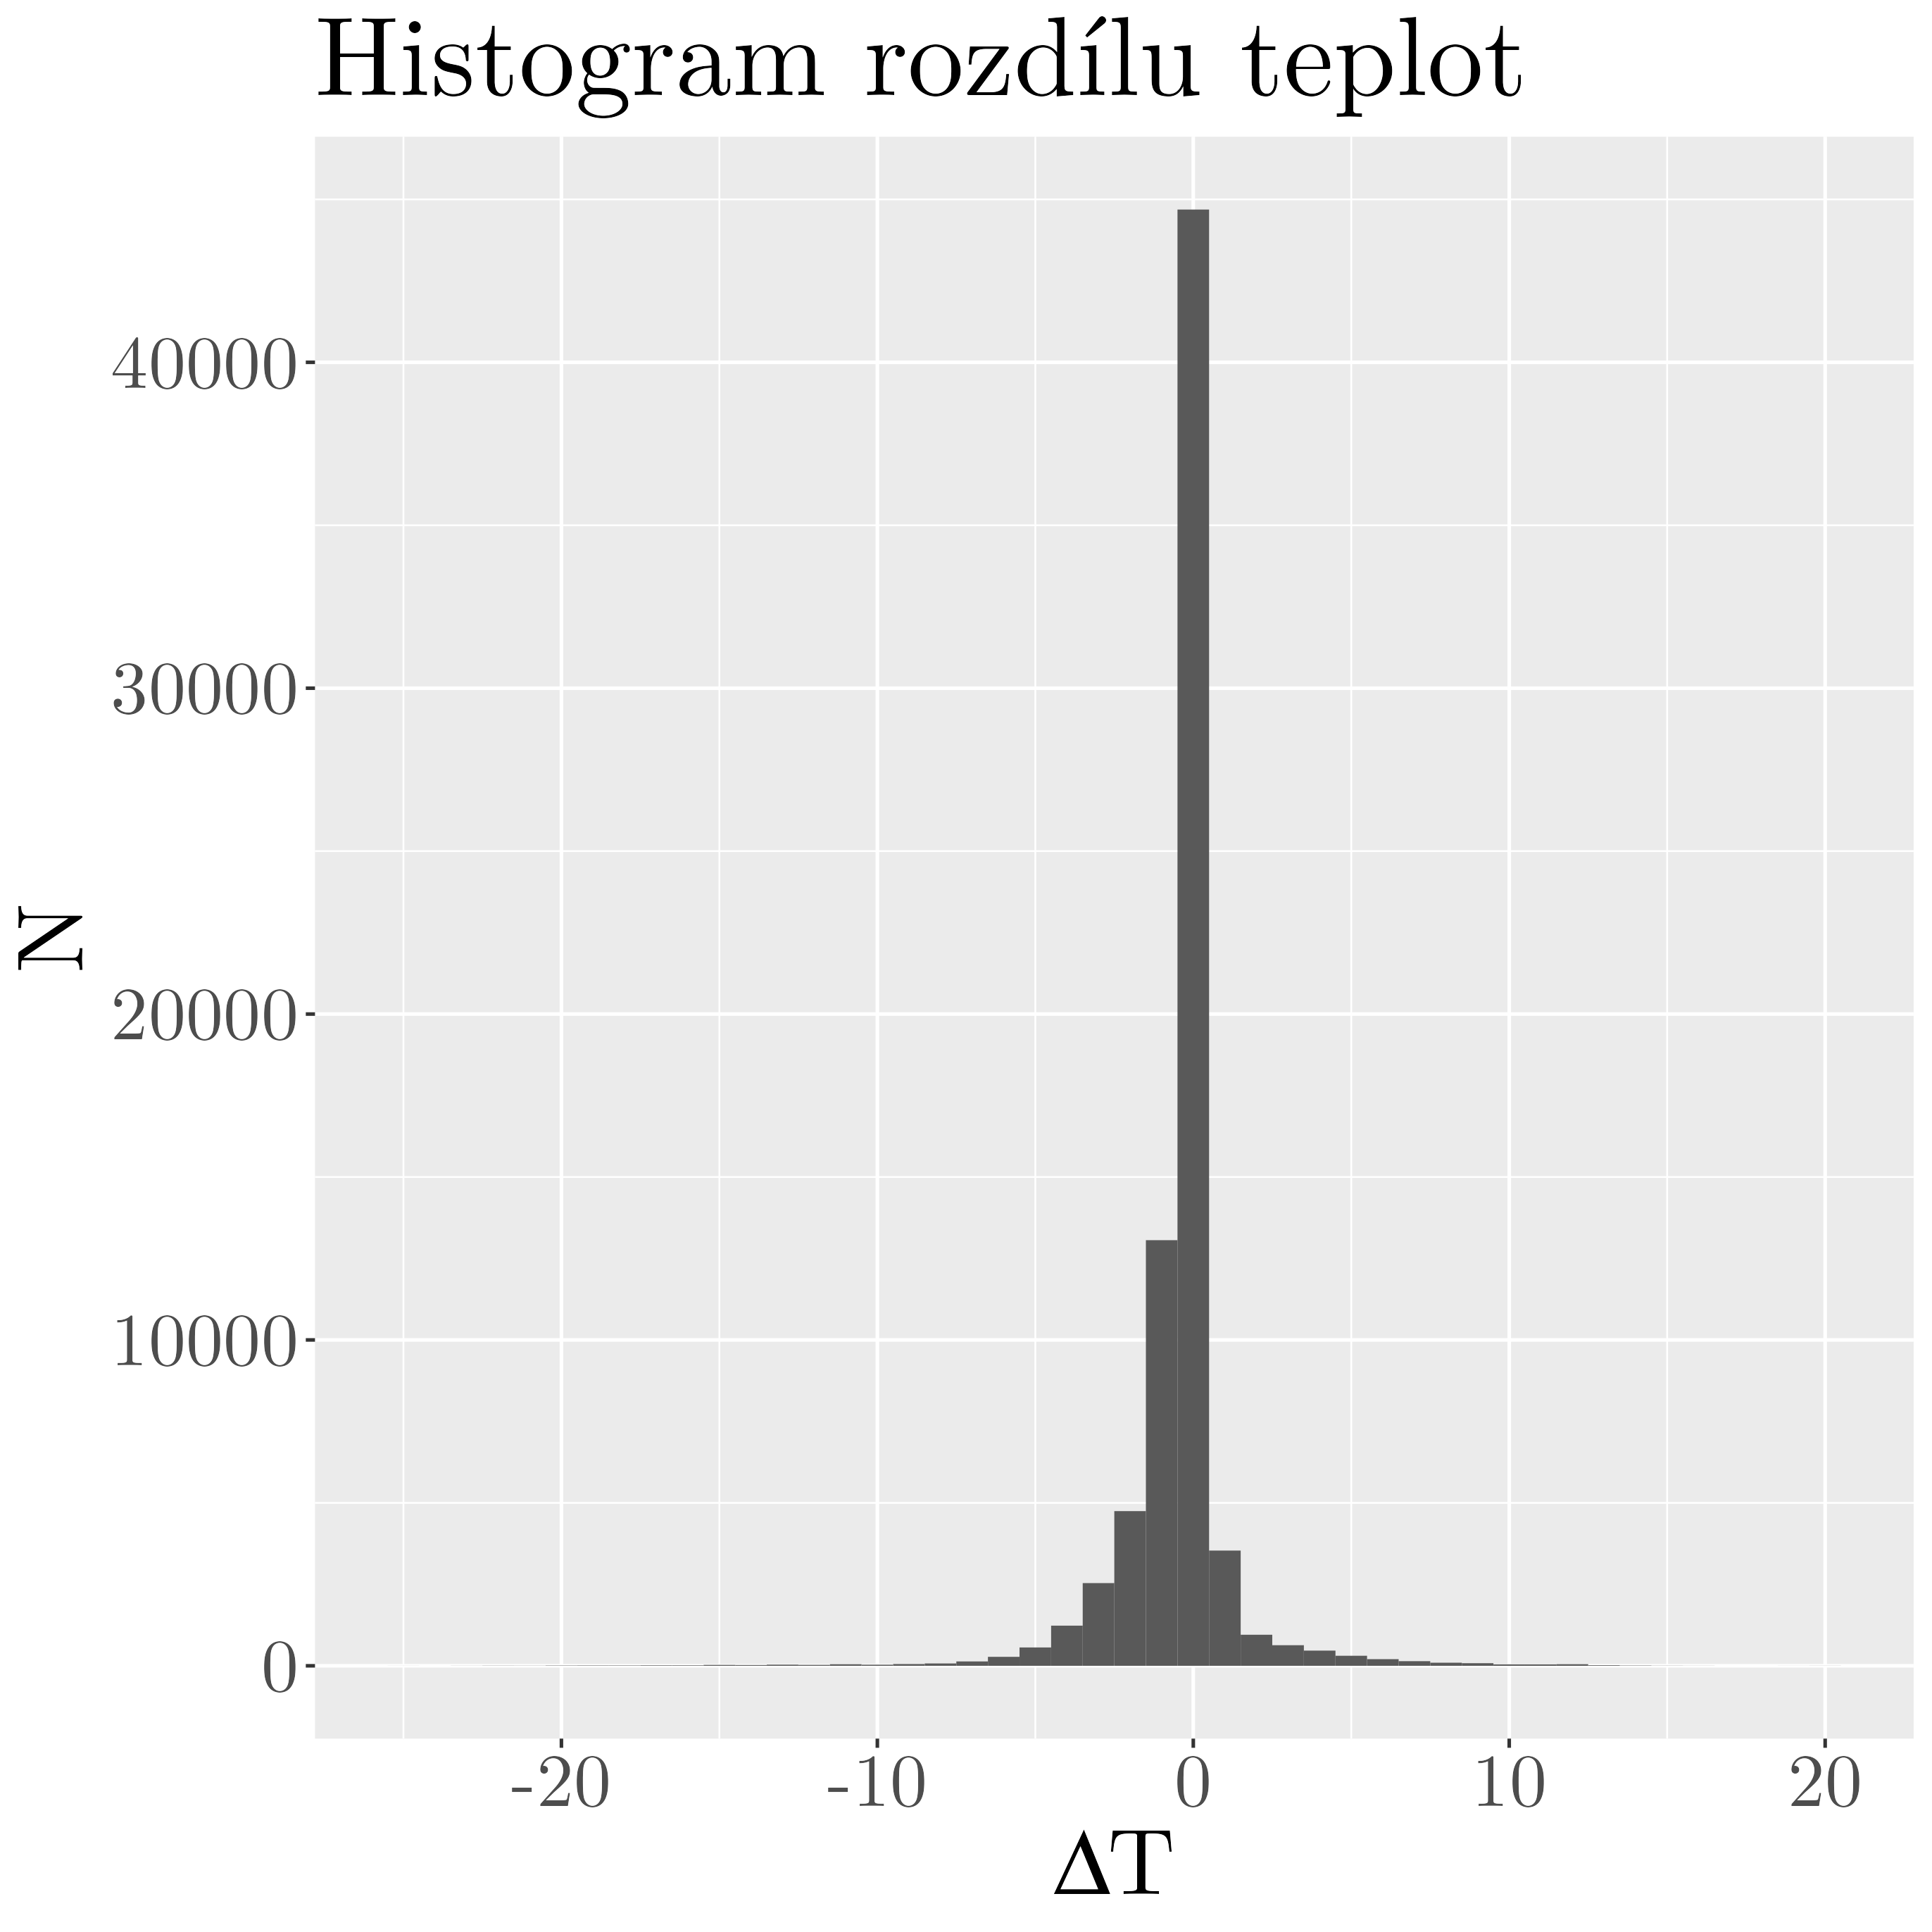
\includegraphics[width=\textwidth]{img/ch2/hist_diff_min15cm.png}
		\caption{Histogram rozdílu minimálních teplot v $\SI{15}{cm}$ a $\SI{2}{m}$. $\text{M} = -0.36$, $\text{MD} = -0.125$.}
		\label{fig:hist_diff_min15cm}
	\end{subfigure}
	\hfill
	\begin{subfigure}{0.45\textwidth}
  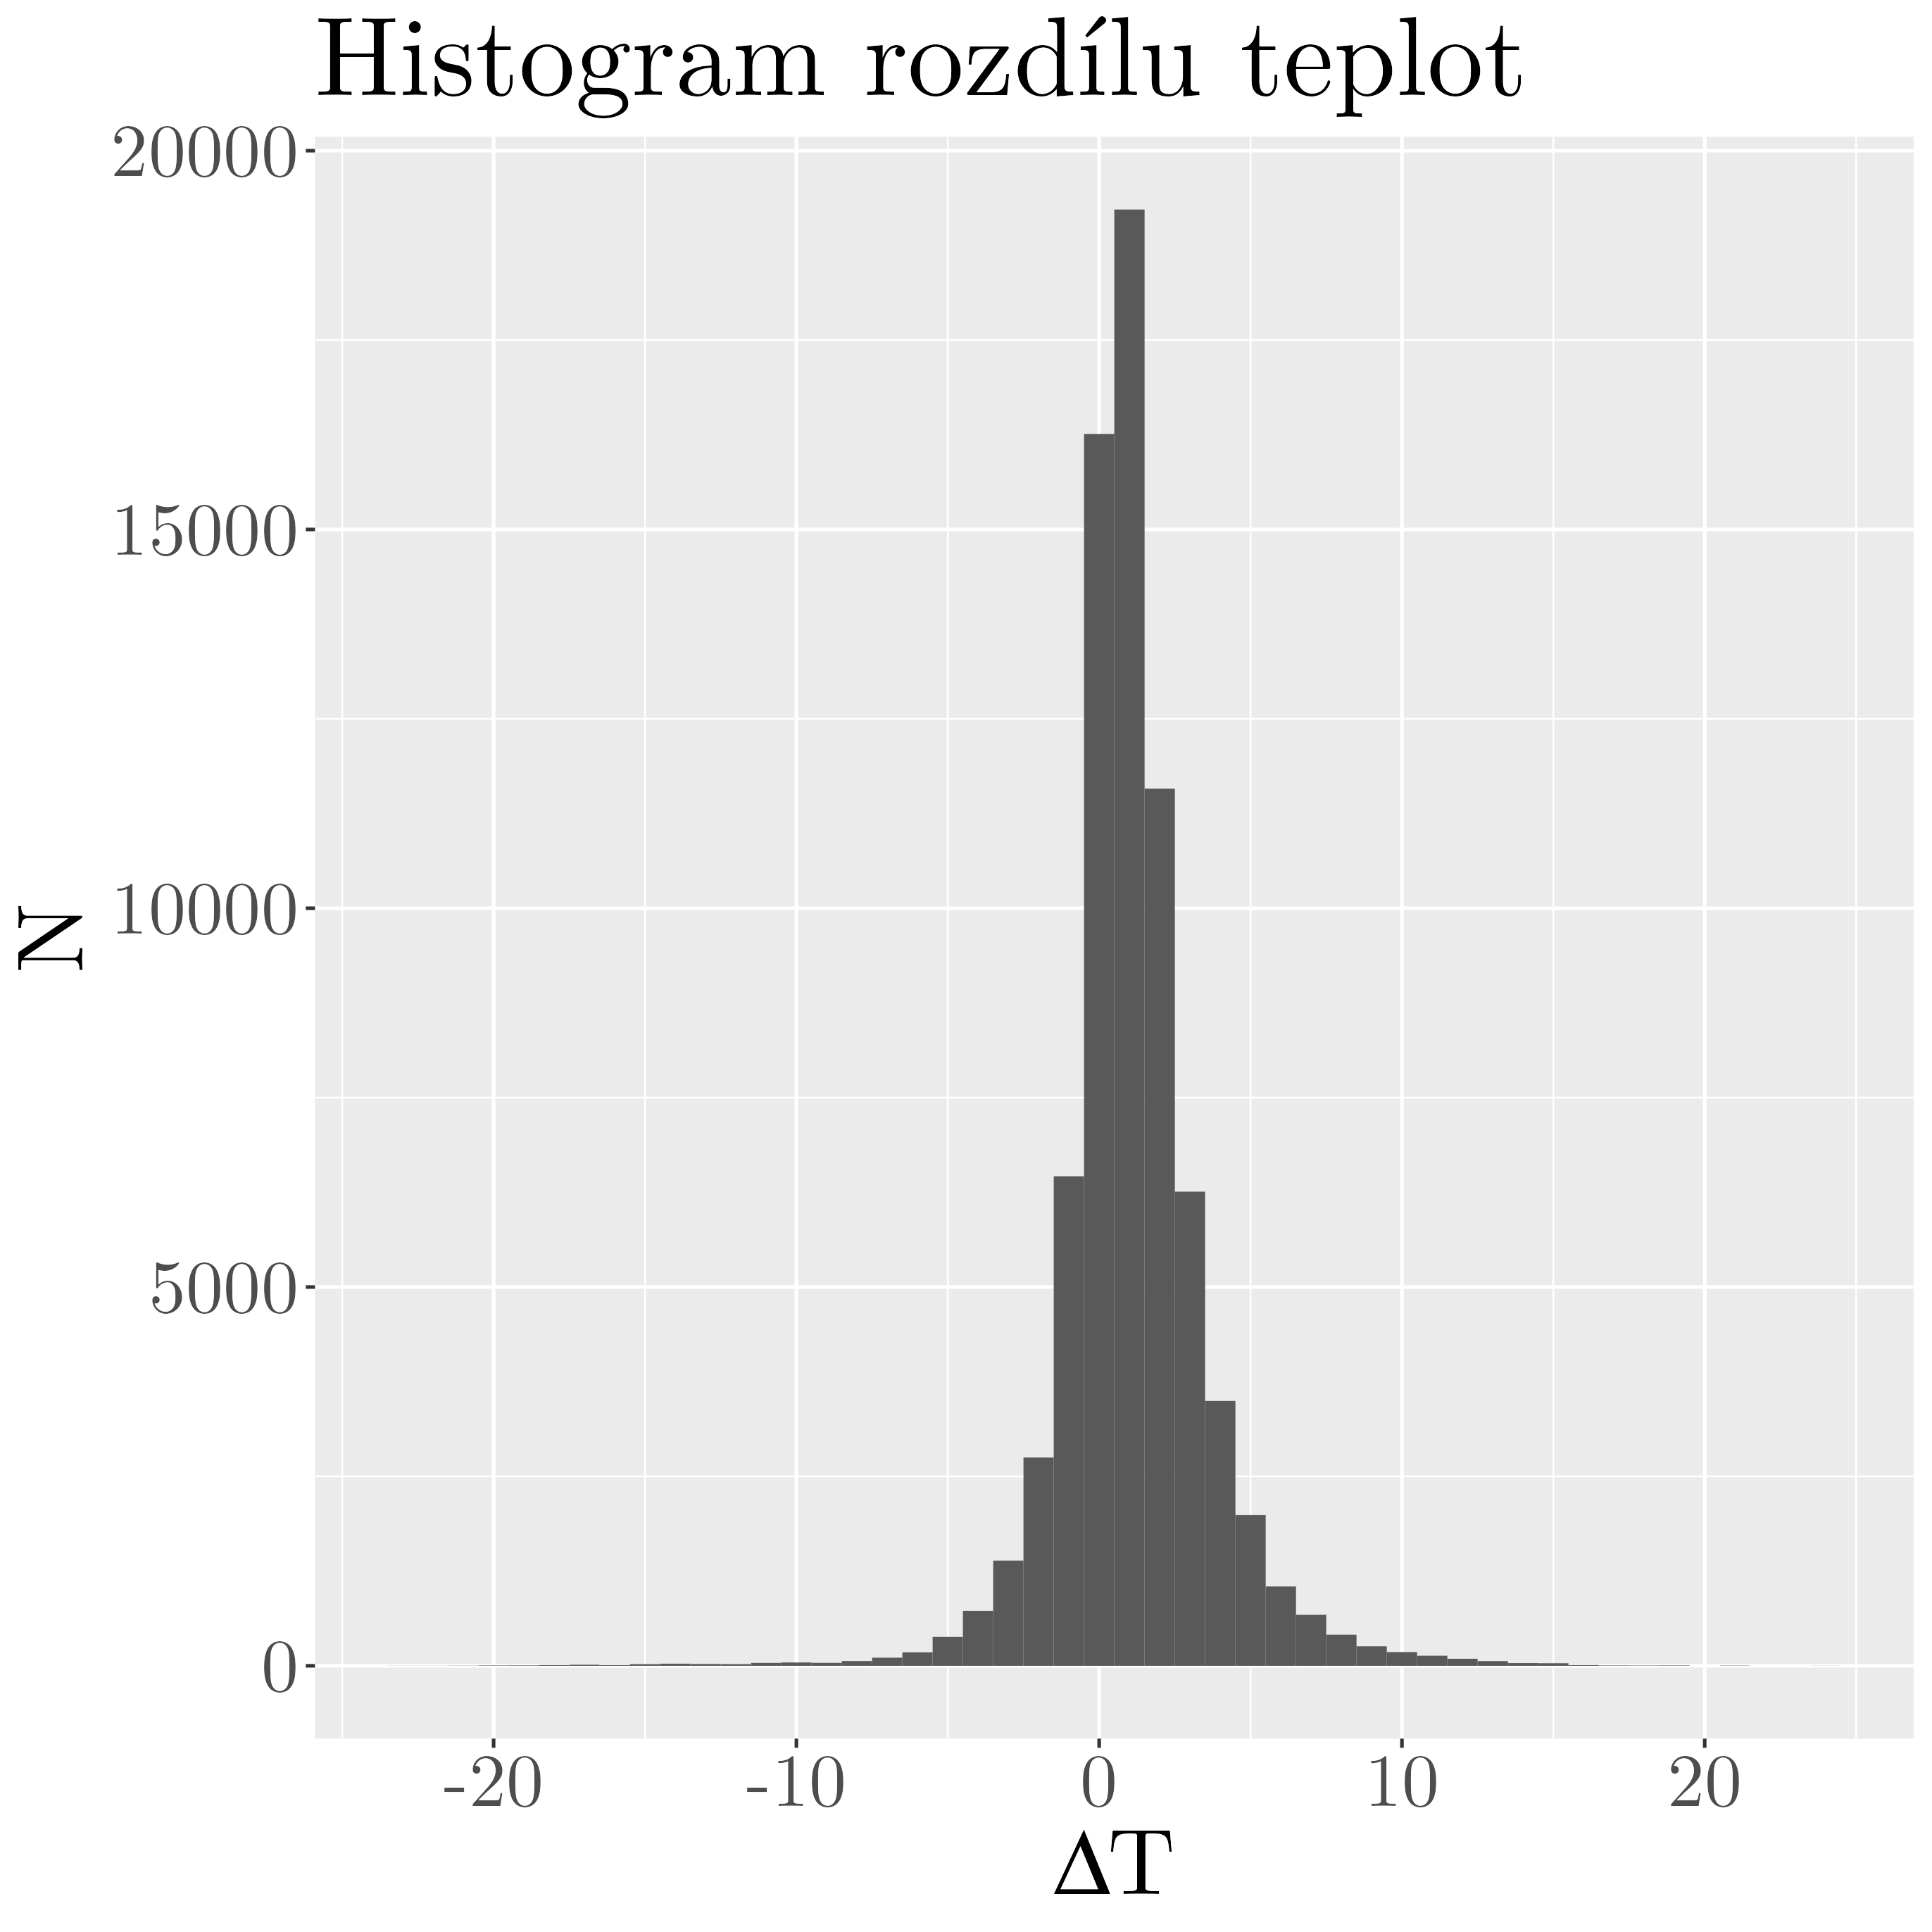
\includegraphics[width=\textwidth]{img/ch2/hist_diff_min0cm.png}
		\caption{Histogram rozdílu miniálních teplot v $\SI{0}{cm}$ a $\SI{2}{m}$. $\text{M} = 1.14$, $\text{MD} = 0.9375$.}
		\label{fig:hist_diff_min0cm}
	\end{subfigure}
	\caption{Histogramy rozdílů maximální, resp. minimální teploty v $\SI{15}{cm}$, resp. v $\SI{0}{cm}$ a ve $\SI{2}{m}$. Ke každému histogramu uvádíme odpovídající hodnotu průměru $\text{M}$ a mediánu $\text{MD}$.}
	\label{fig:hist_diff}
\end{figure}


\section{Metody analýzy dat}\label{chap:methods}
Cílem následující části je ukázat jakým způsobem byla data zpracována, proč byl vybrán daný model a ukázat ověření metody ověření předpokladů.

\subsection{Korelace dat}
Z povahy naměřených dat je zřejmé, že zde existuje autokorelace mezi naměřenými maximálními nebo minimálními teplotami. Autokorelace se pak projevuje i u rozdílu teploty naměřené blízko země a ve $\SI{2}{m}$. Na obrázku \ref{fig:acf} vidíme autokorelační funkci pro jedno z čidel.

\begin{figure}
	\centering
	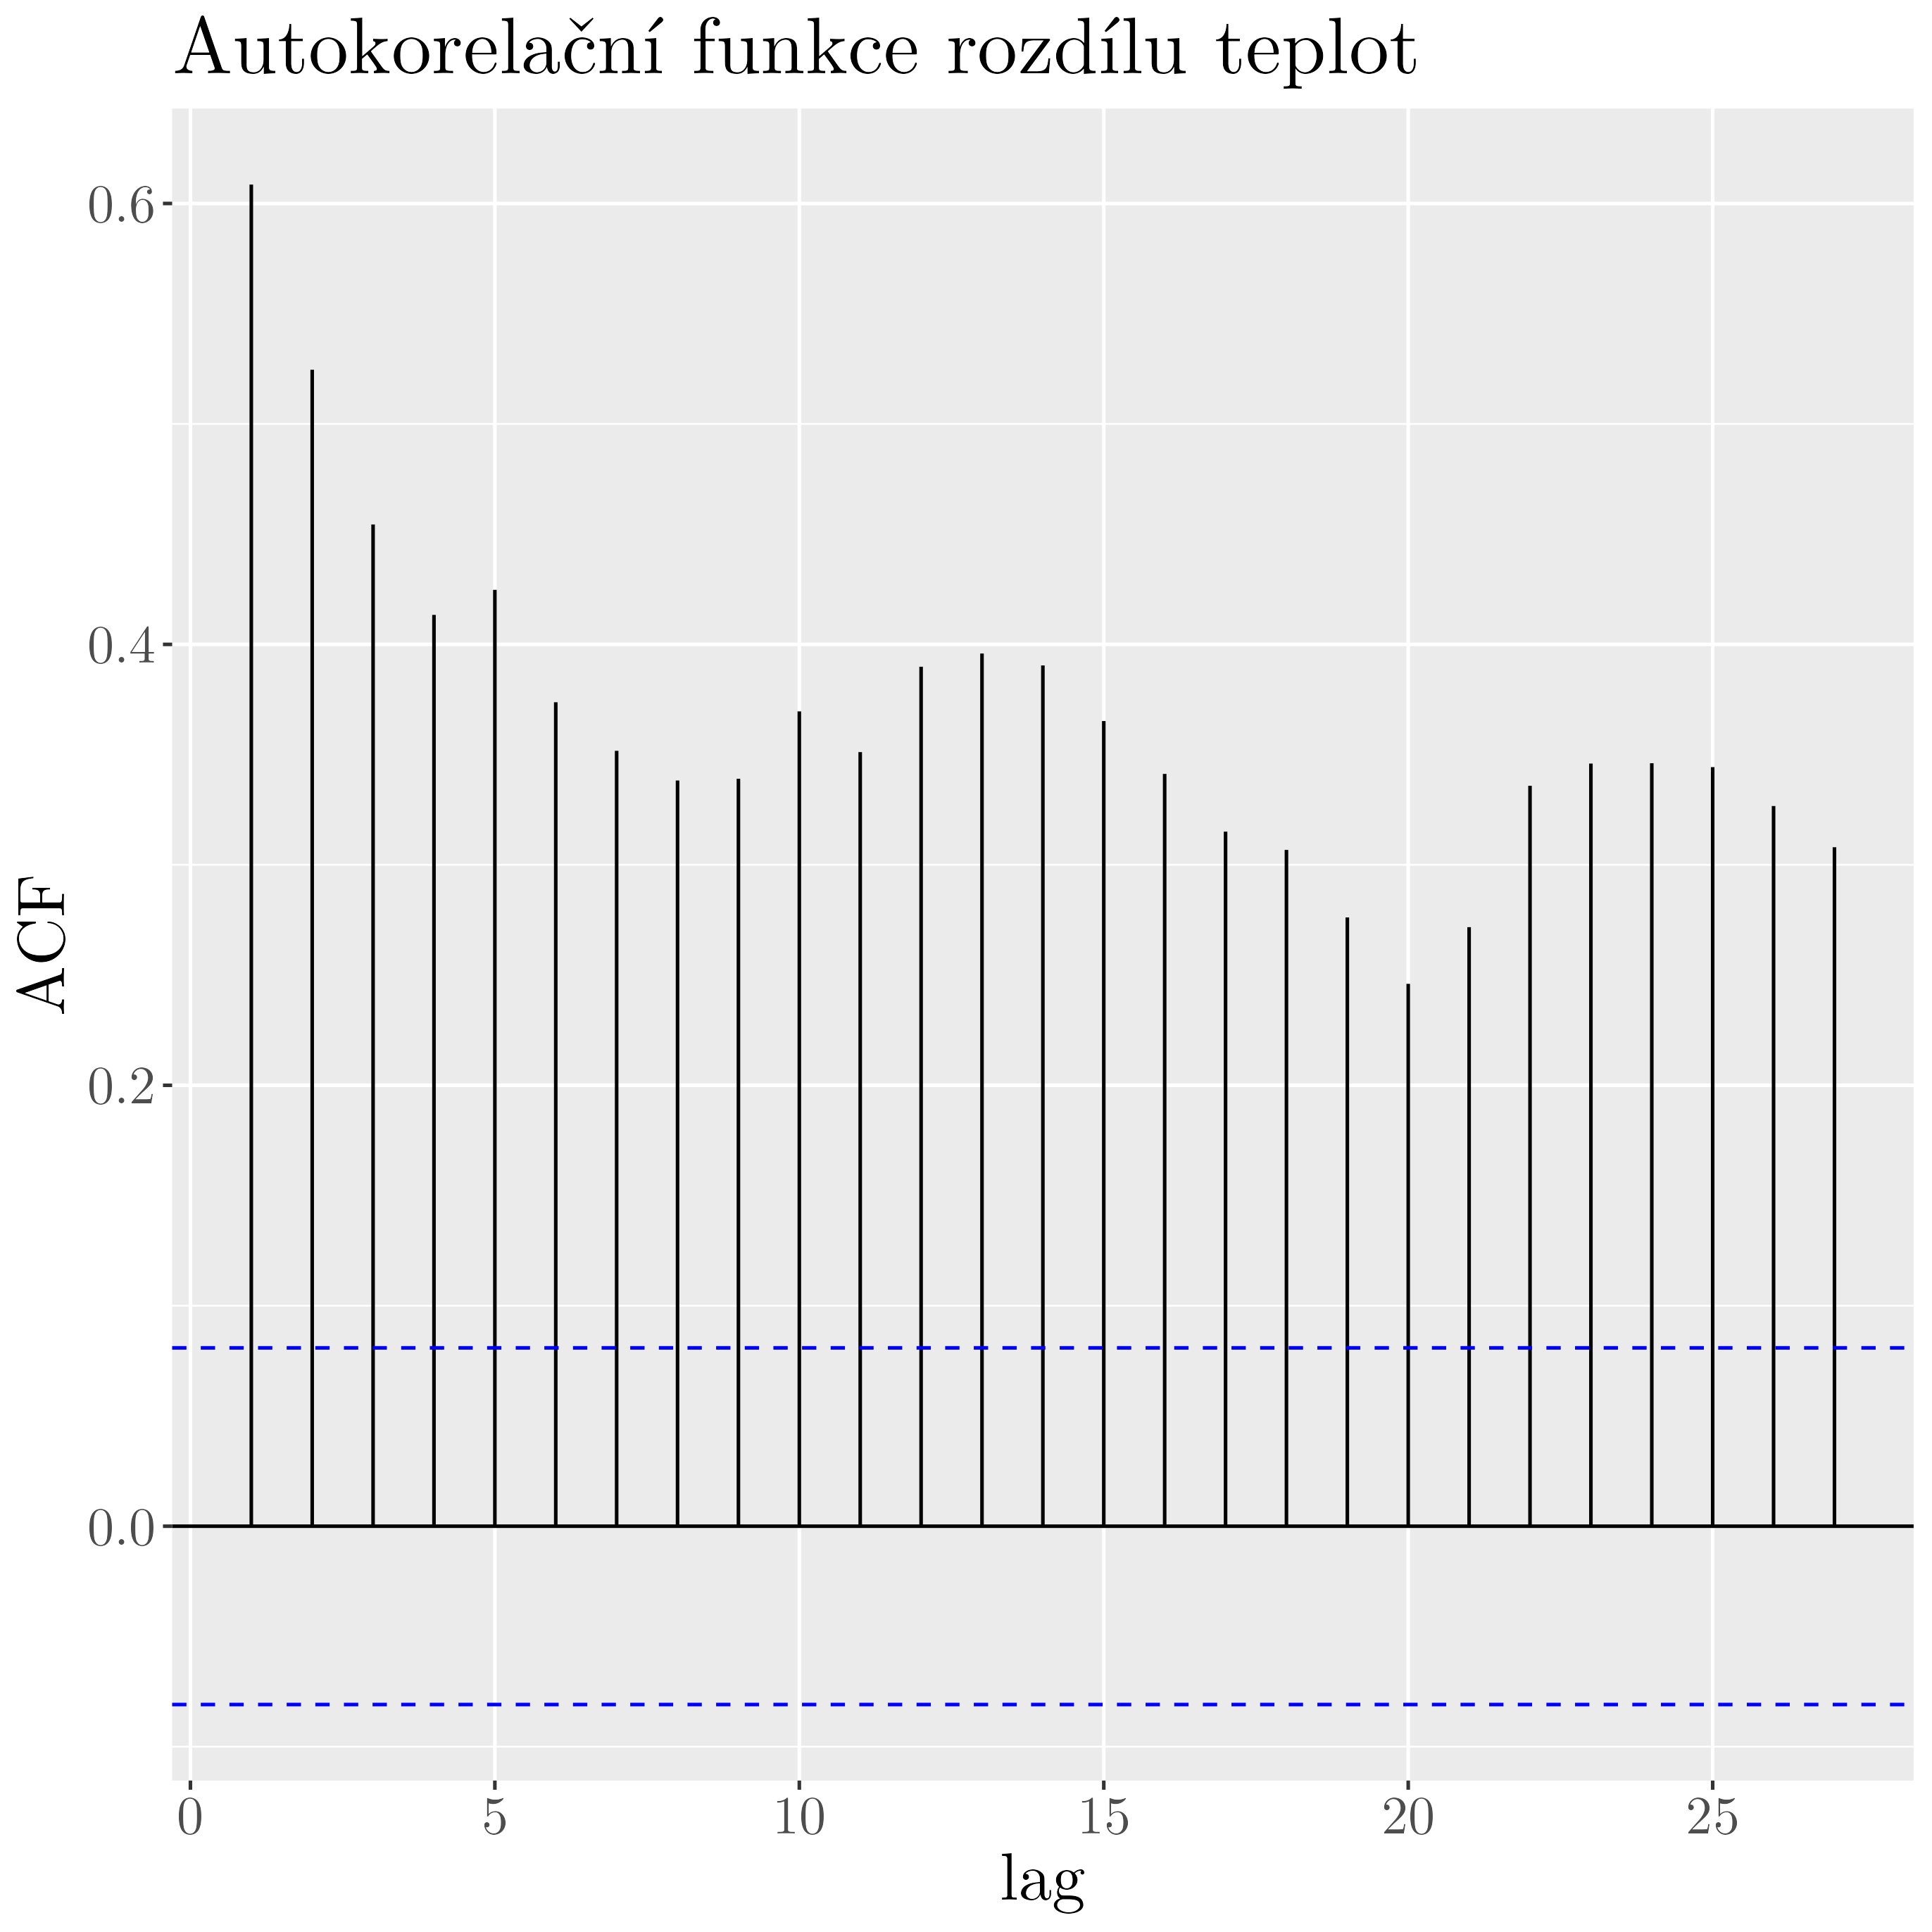
\includegraphics[width=0.55\textwidth]{img/ch2/acfNPS_4311_D_TMS.png}
	\caption{Autokorelační funkce pro rozdíl teplot mezi maximální teplotou v $\SI{15}{cm}$ a teplotou ve $\SI{2}{m}$ na páru čidel nejblíže meteorologické stanici Churáňov.}
	\label{fig:acf}
\end{figure}

Autokorelace není takto významná pro všechna čidla, ale i tak nám vylučuje možnost využít jednoduché mnohonásobné lineární regrese.

Kvůli prostorové struktuře dat musíme otestovat prostorovou korelaci. Využijeme teorii popsanou v kapitole \ref{chap:variogram}. Na obrázcích \ref{fig:variograms} vidíme dvanáct semivariogramů pro každý první den měsíce v roce 2020. Kvůli lišícím se hodnotám semivariance nemůžeme semivariogramy zakreslit do jednoho grafu. Ze semivariogramů můžeme usoudit, že v datech neexistuje významná prostorová korelace, kterou bychom museli v modelu zohlednit (prostorovou korelaci, bychom očekávali hlavně v prvních deseti kilometrech viz kapitola \ref{chap:variogram}).

\begin{figure}
	\centering
	\begin{subfigure}{0.30\textwidth}
		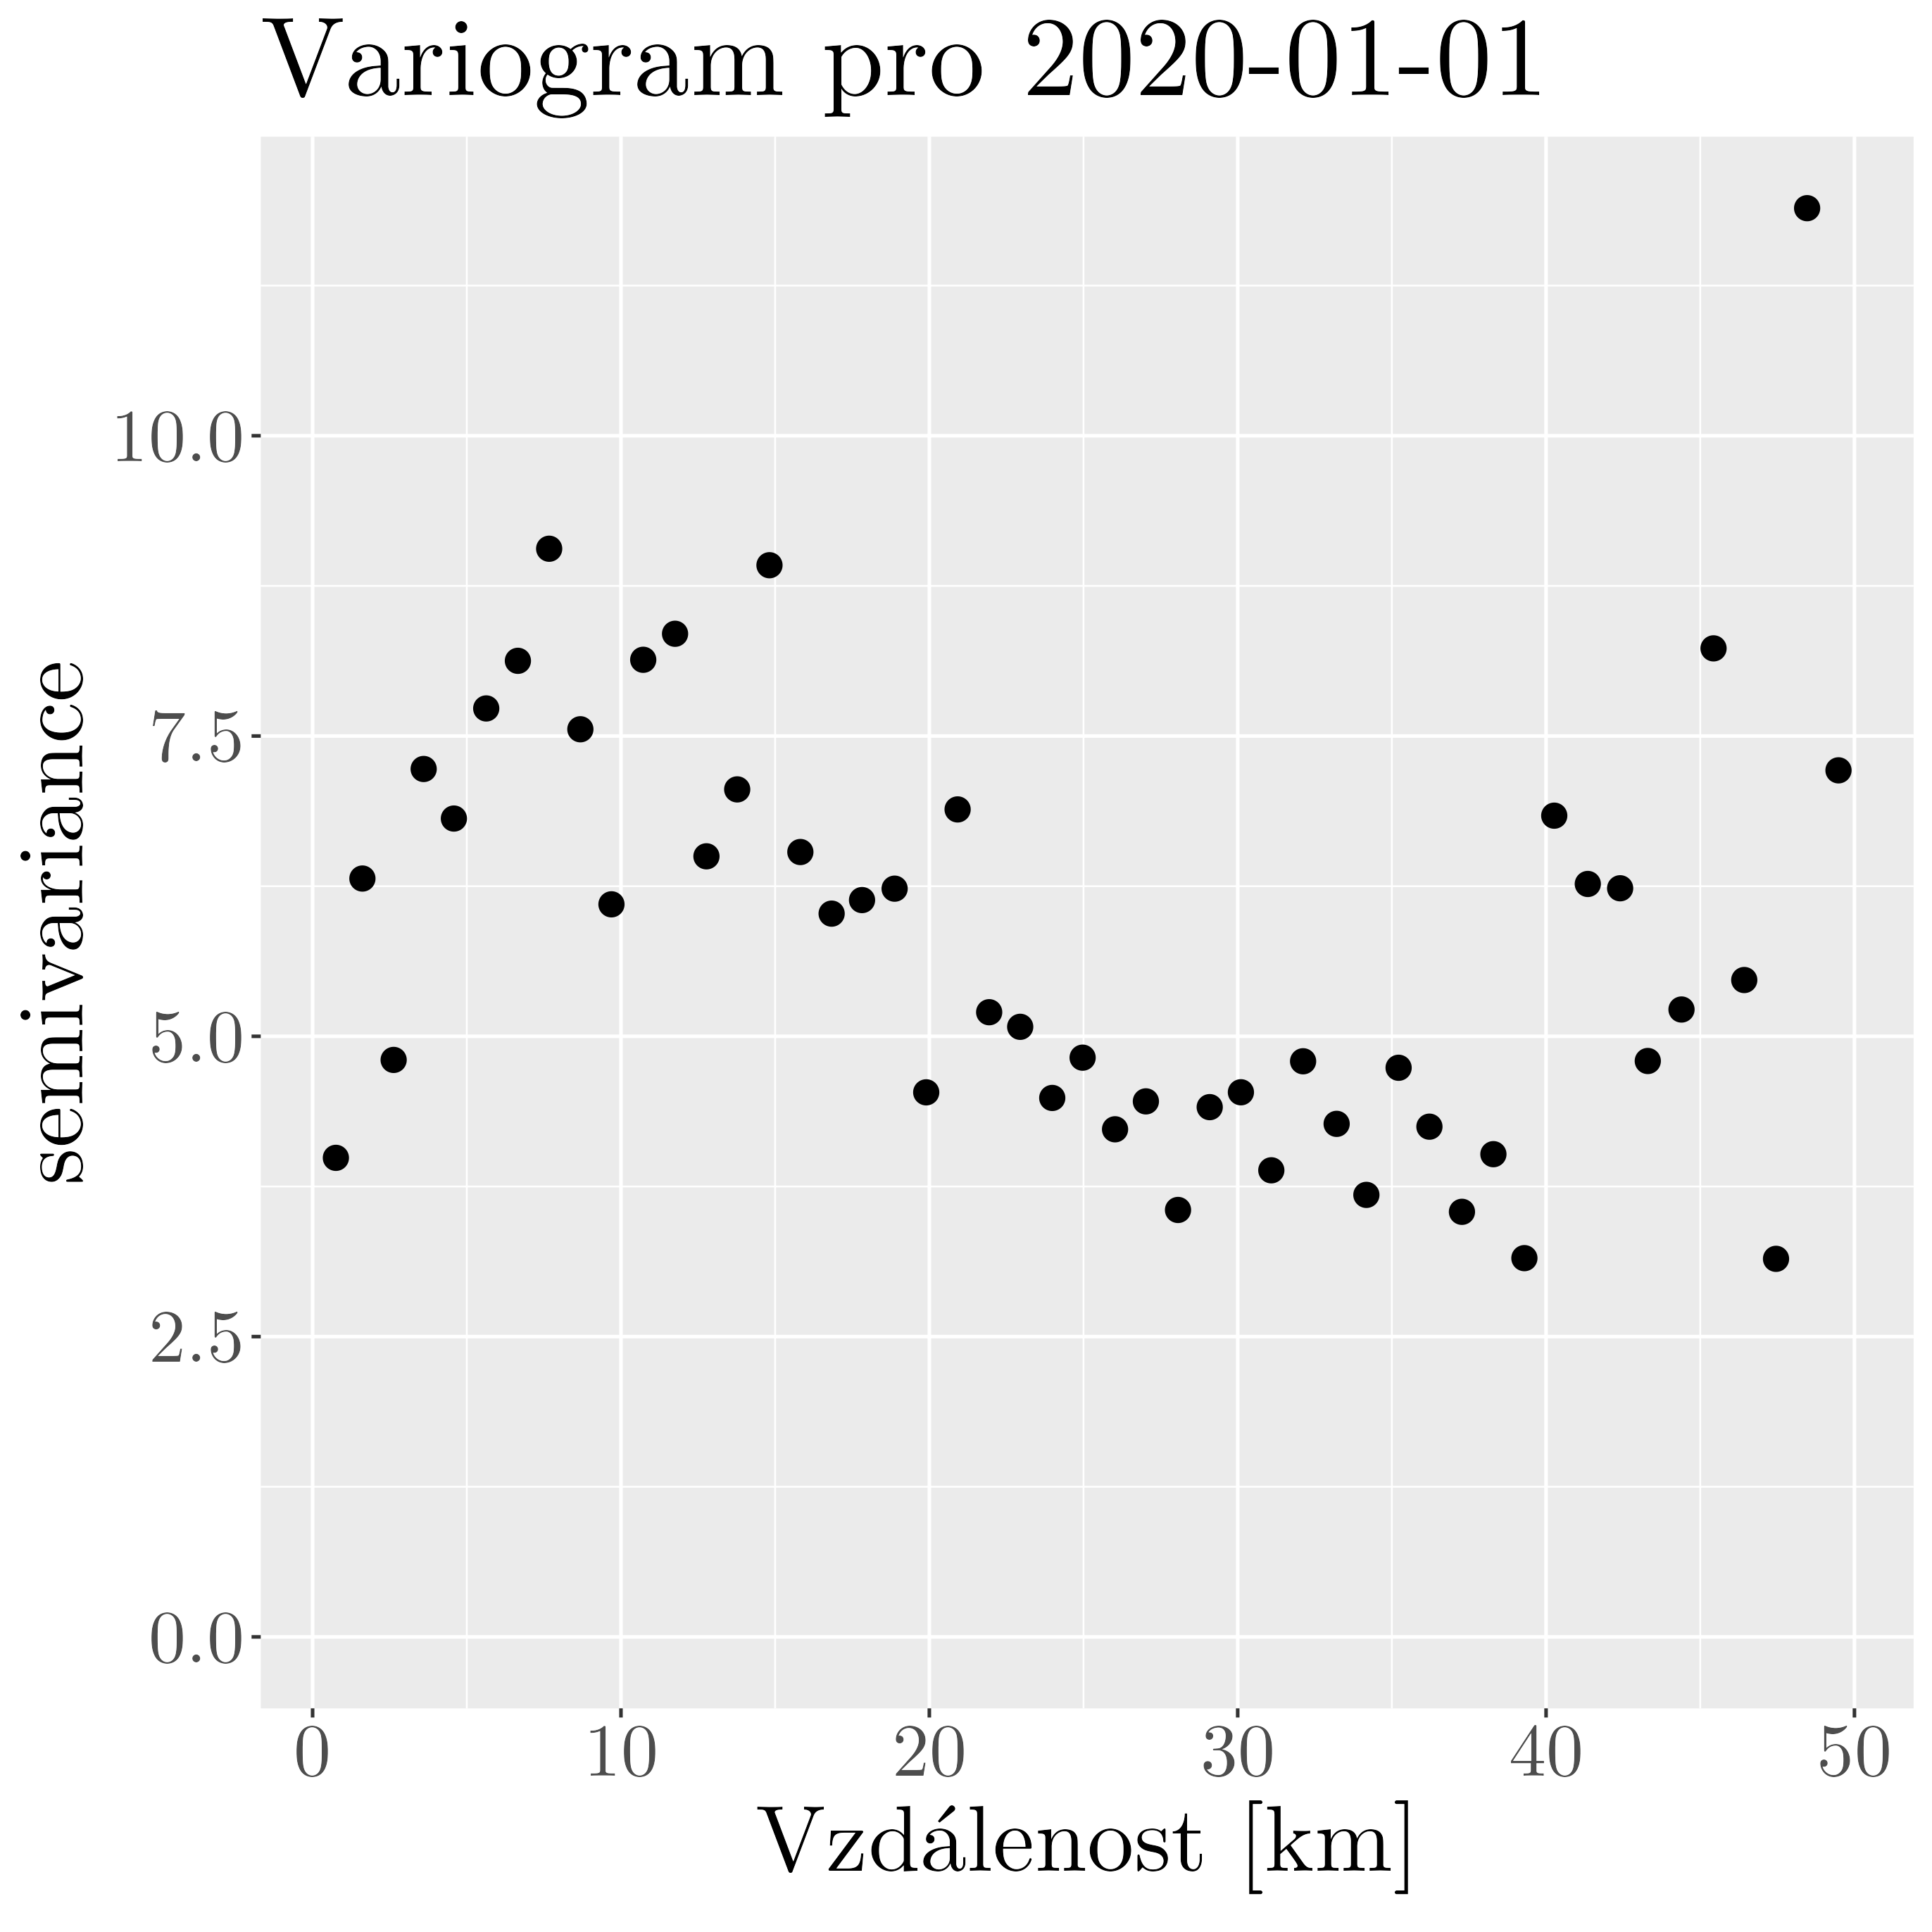
\includegraphics[width=\textwidth]{img/ch2/variograms/variogram_max15cm1.png}
		\caption{}
		\label{fig:variogram1}
	\end{subfigure}
	\hfill
	\begin{subfigure}{0.30\textwidth}
		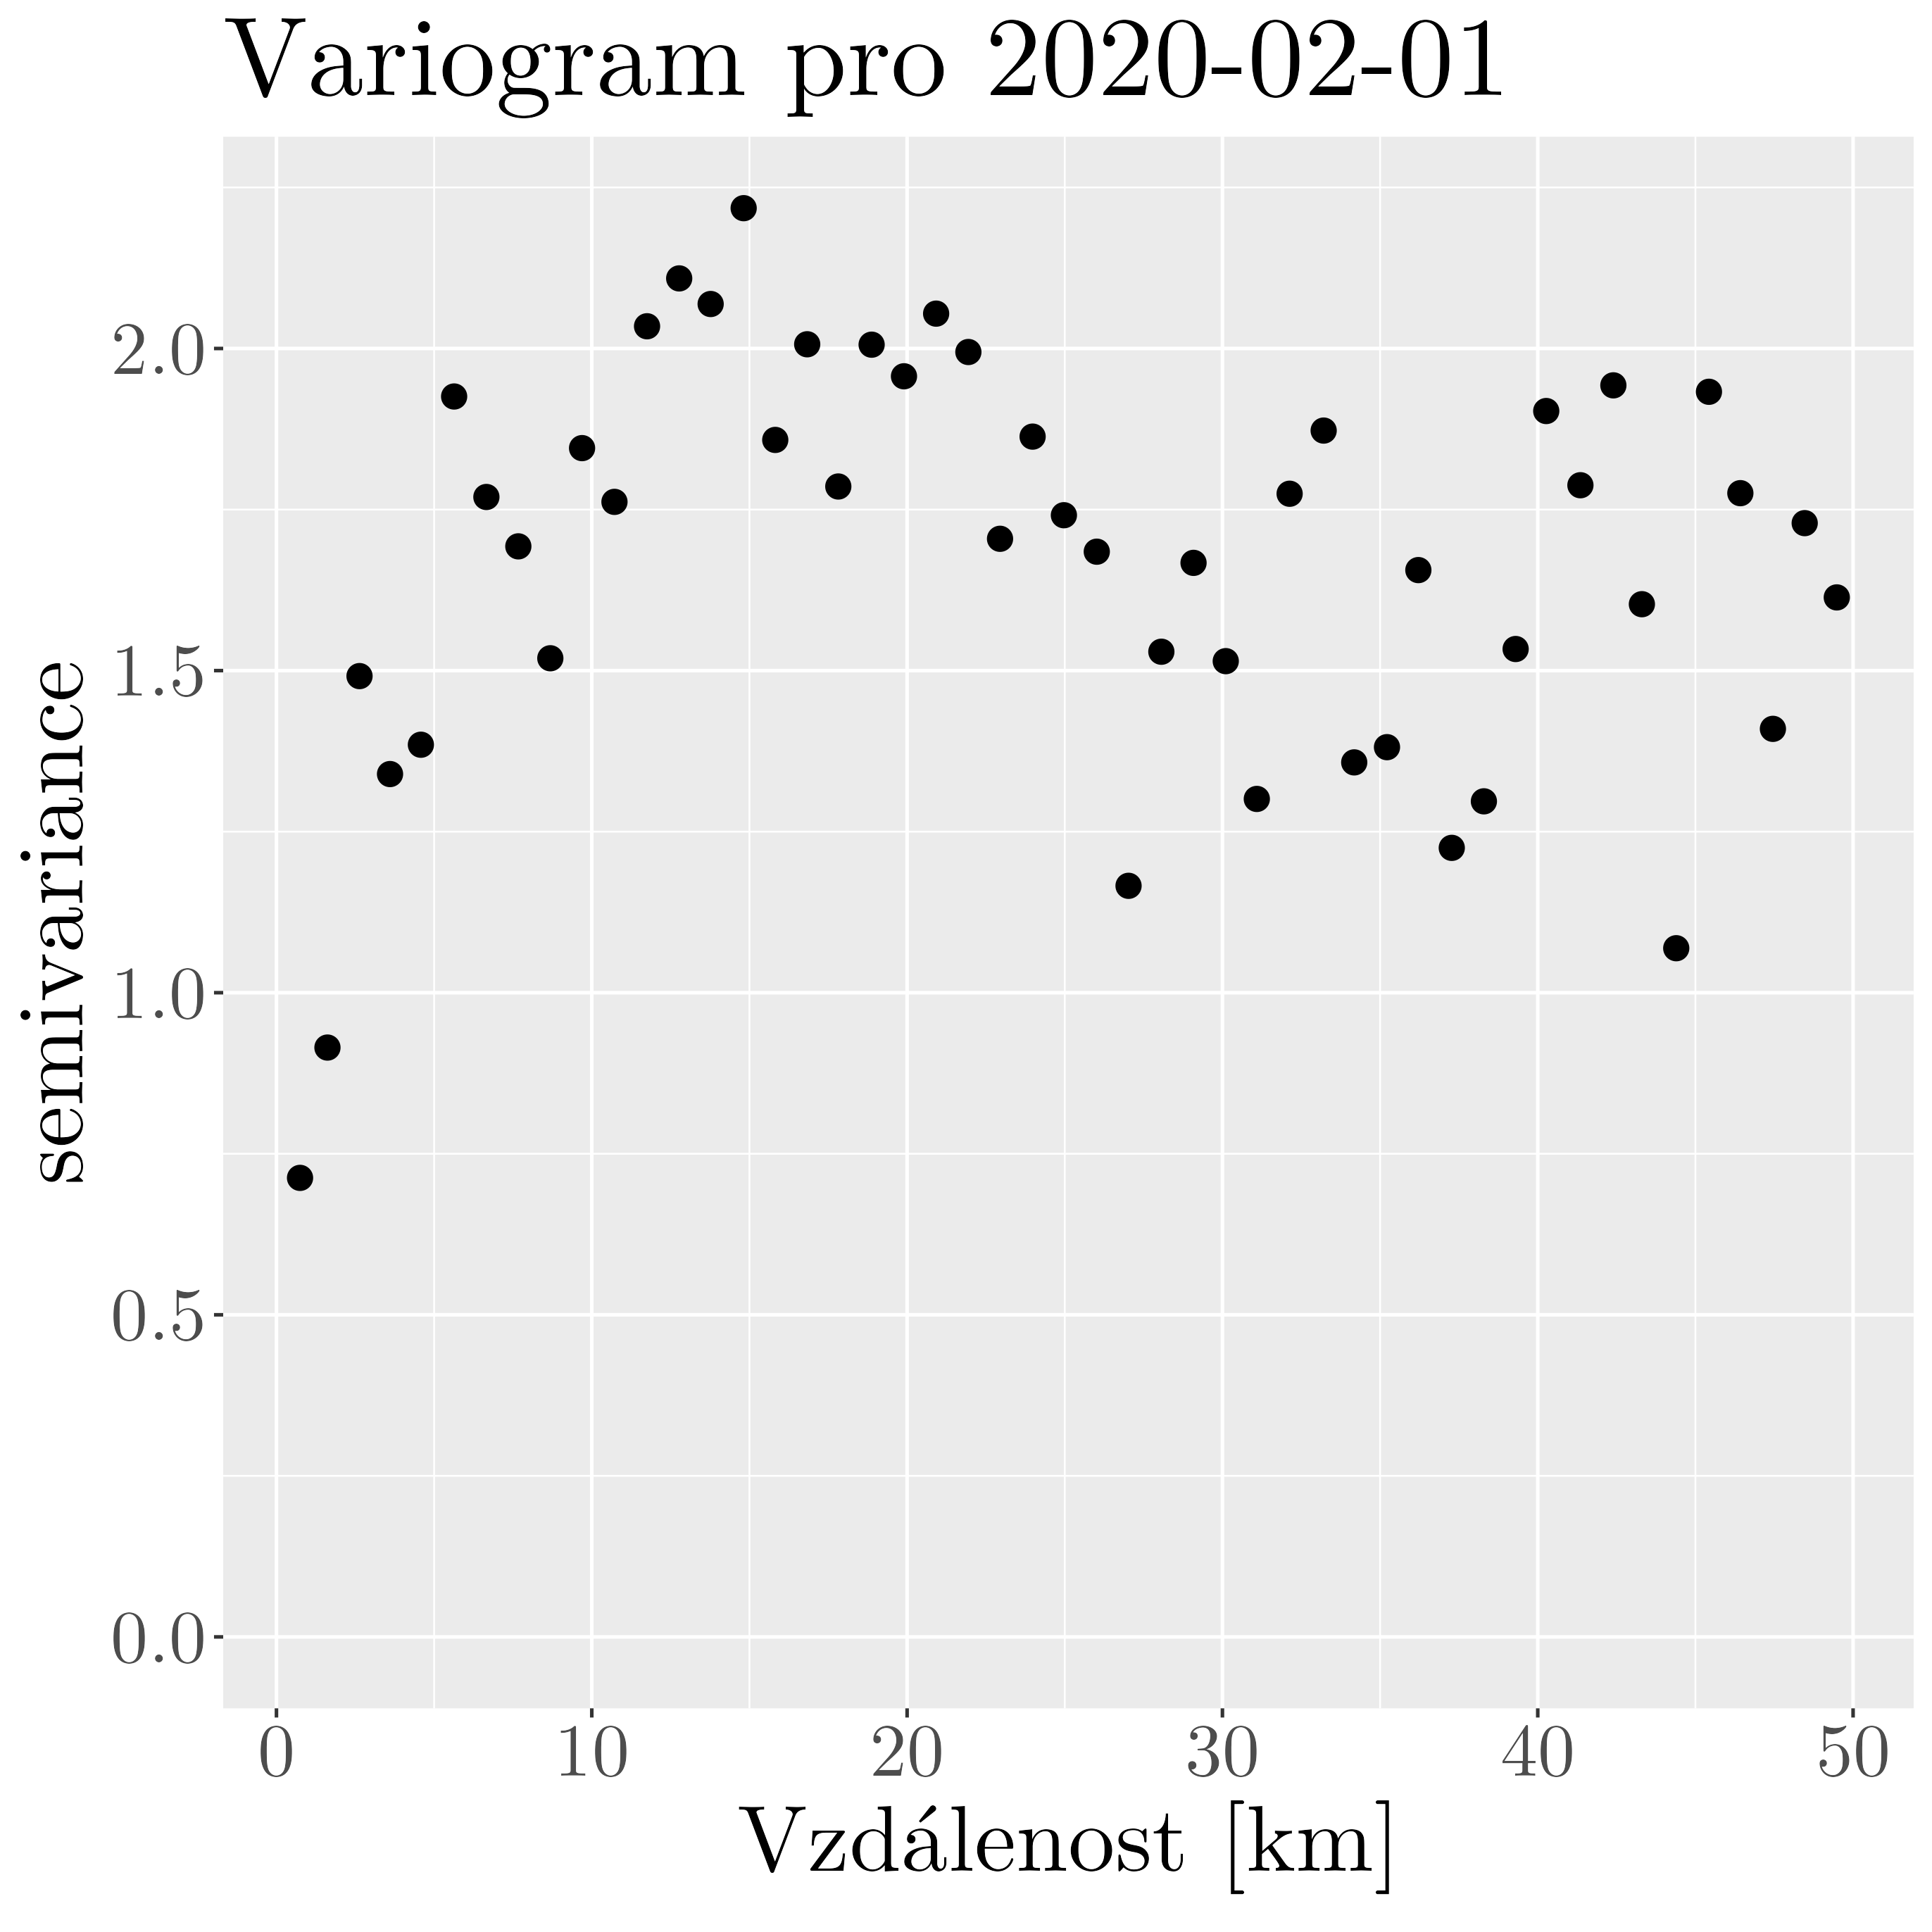
\includegraphics[width=\textwidth]{img/ch2/variograms/variogram_max15cm2.png}
		\caption{}
		\label{fig:variogram2}
	\end{subfigure}
	\hfill
	\begin{subfigure}{0.30\textwidth}
		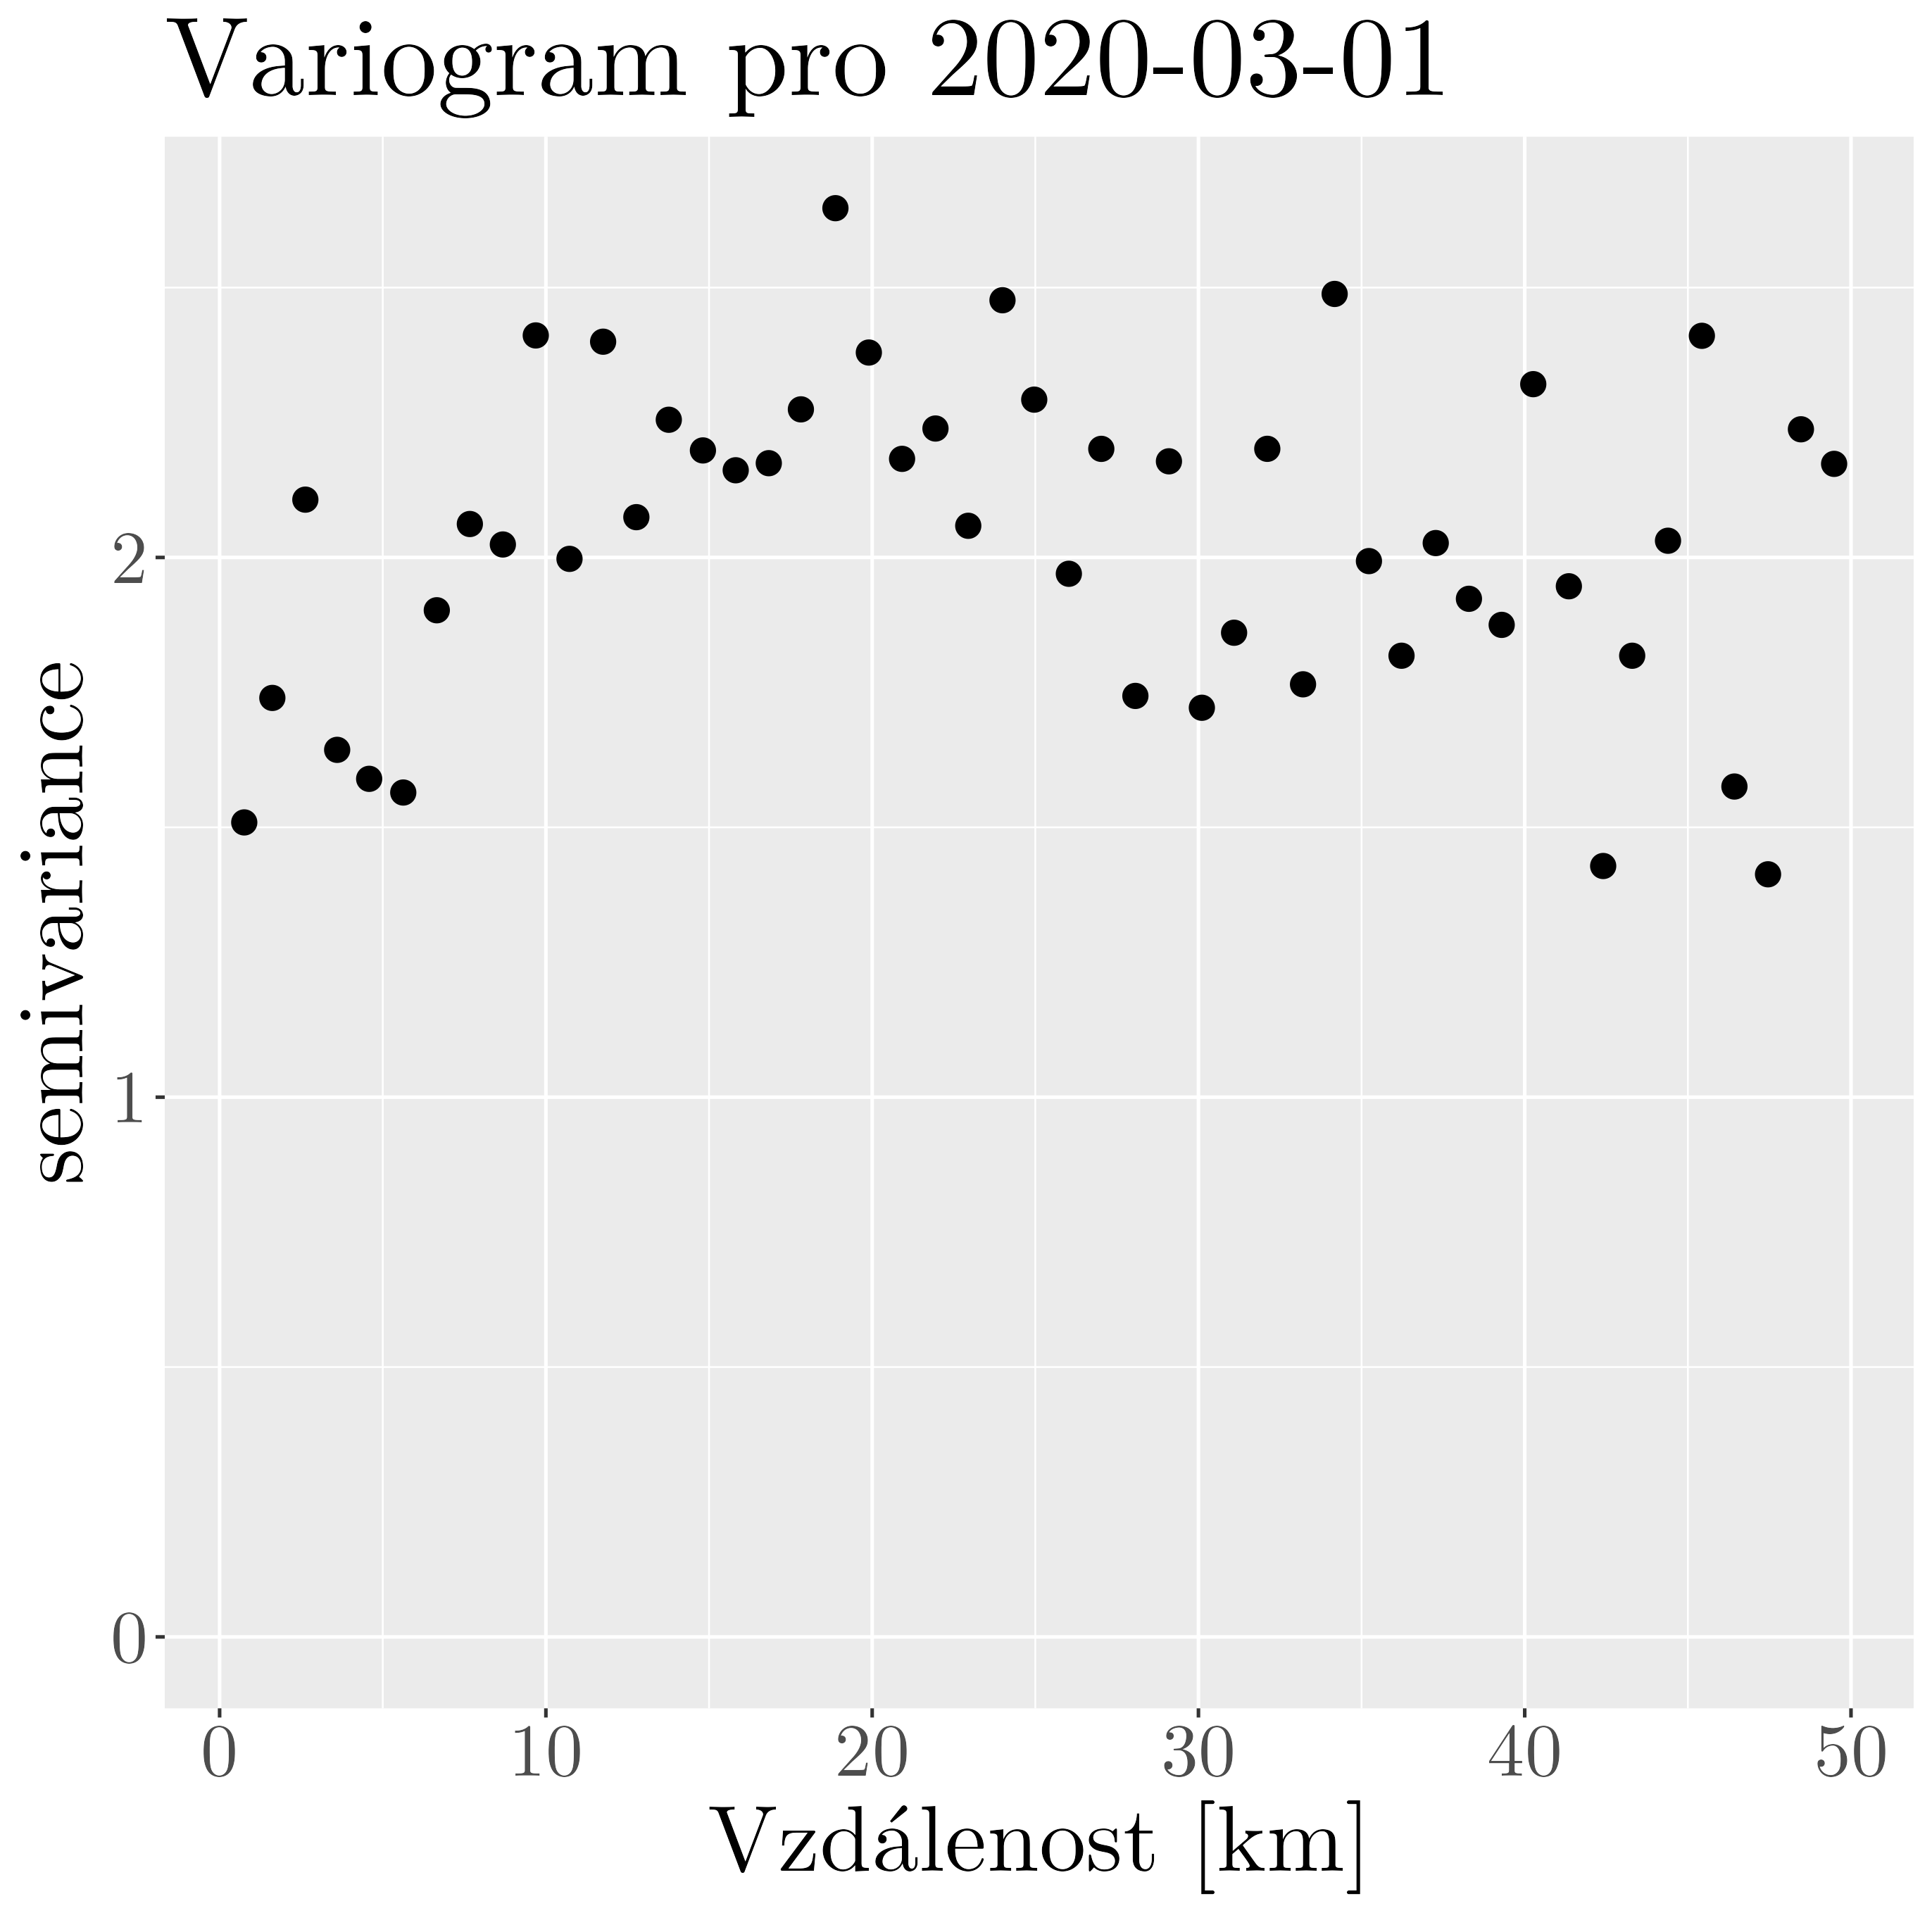
\includegraphics[width=\textwidth]{img/ch2/variograms/variogram_max15cm3.png}
		\caption{}
		\label{fig:variogram3}
	\end{subfigure}
	\hfill
	\begin{subfigure}{0.30\textwidth}
		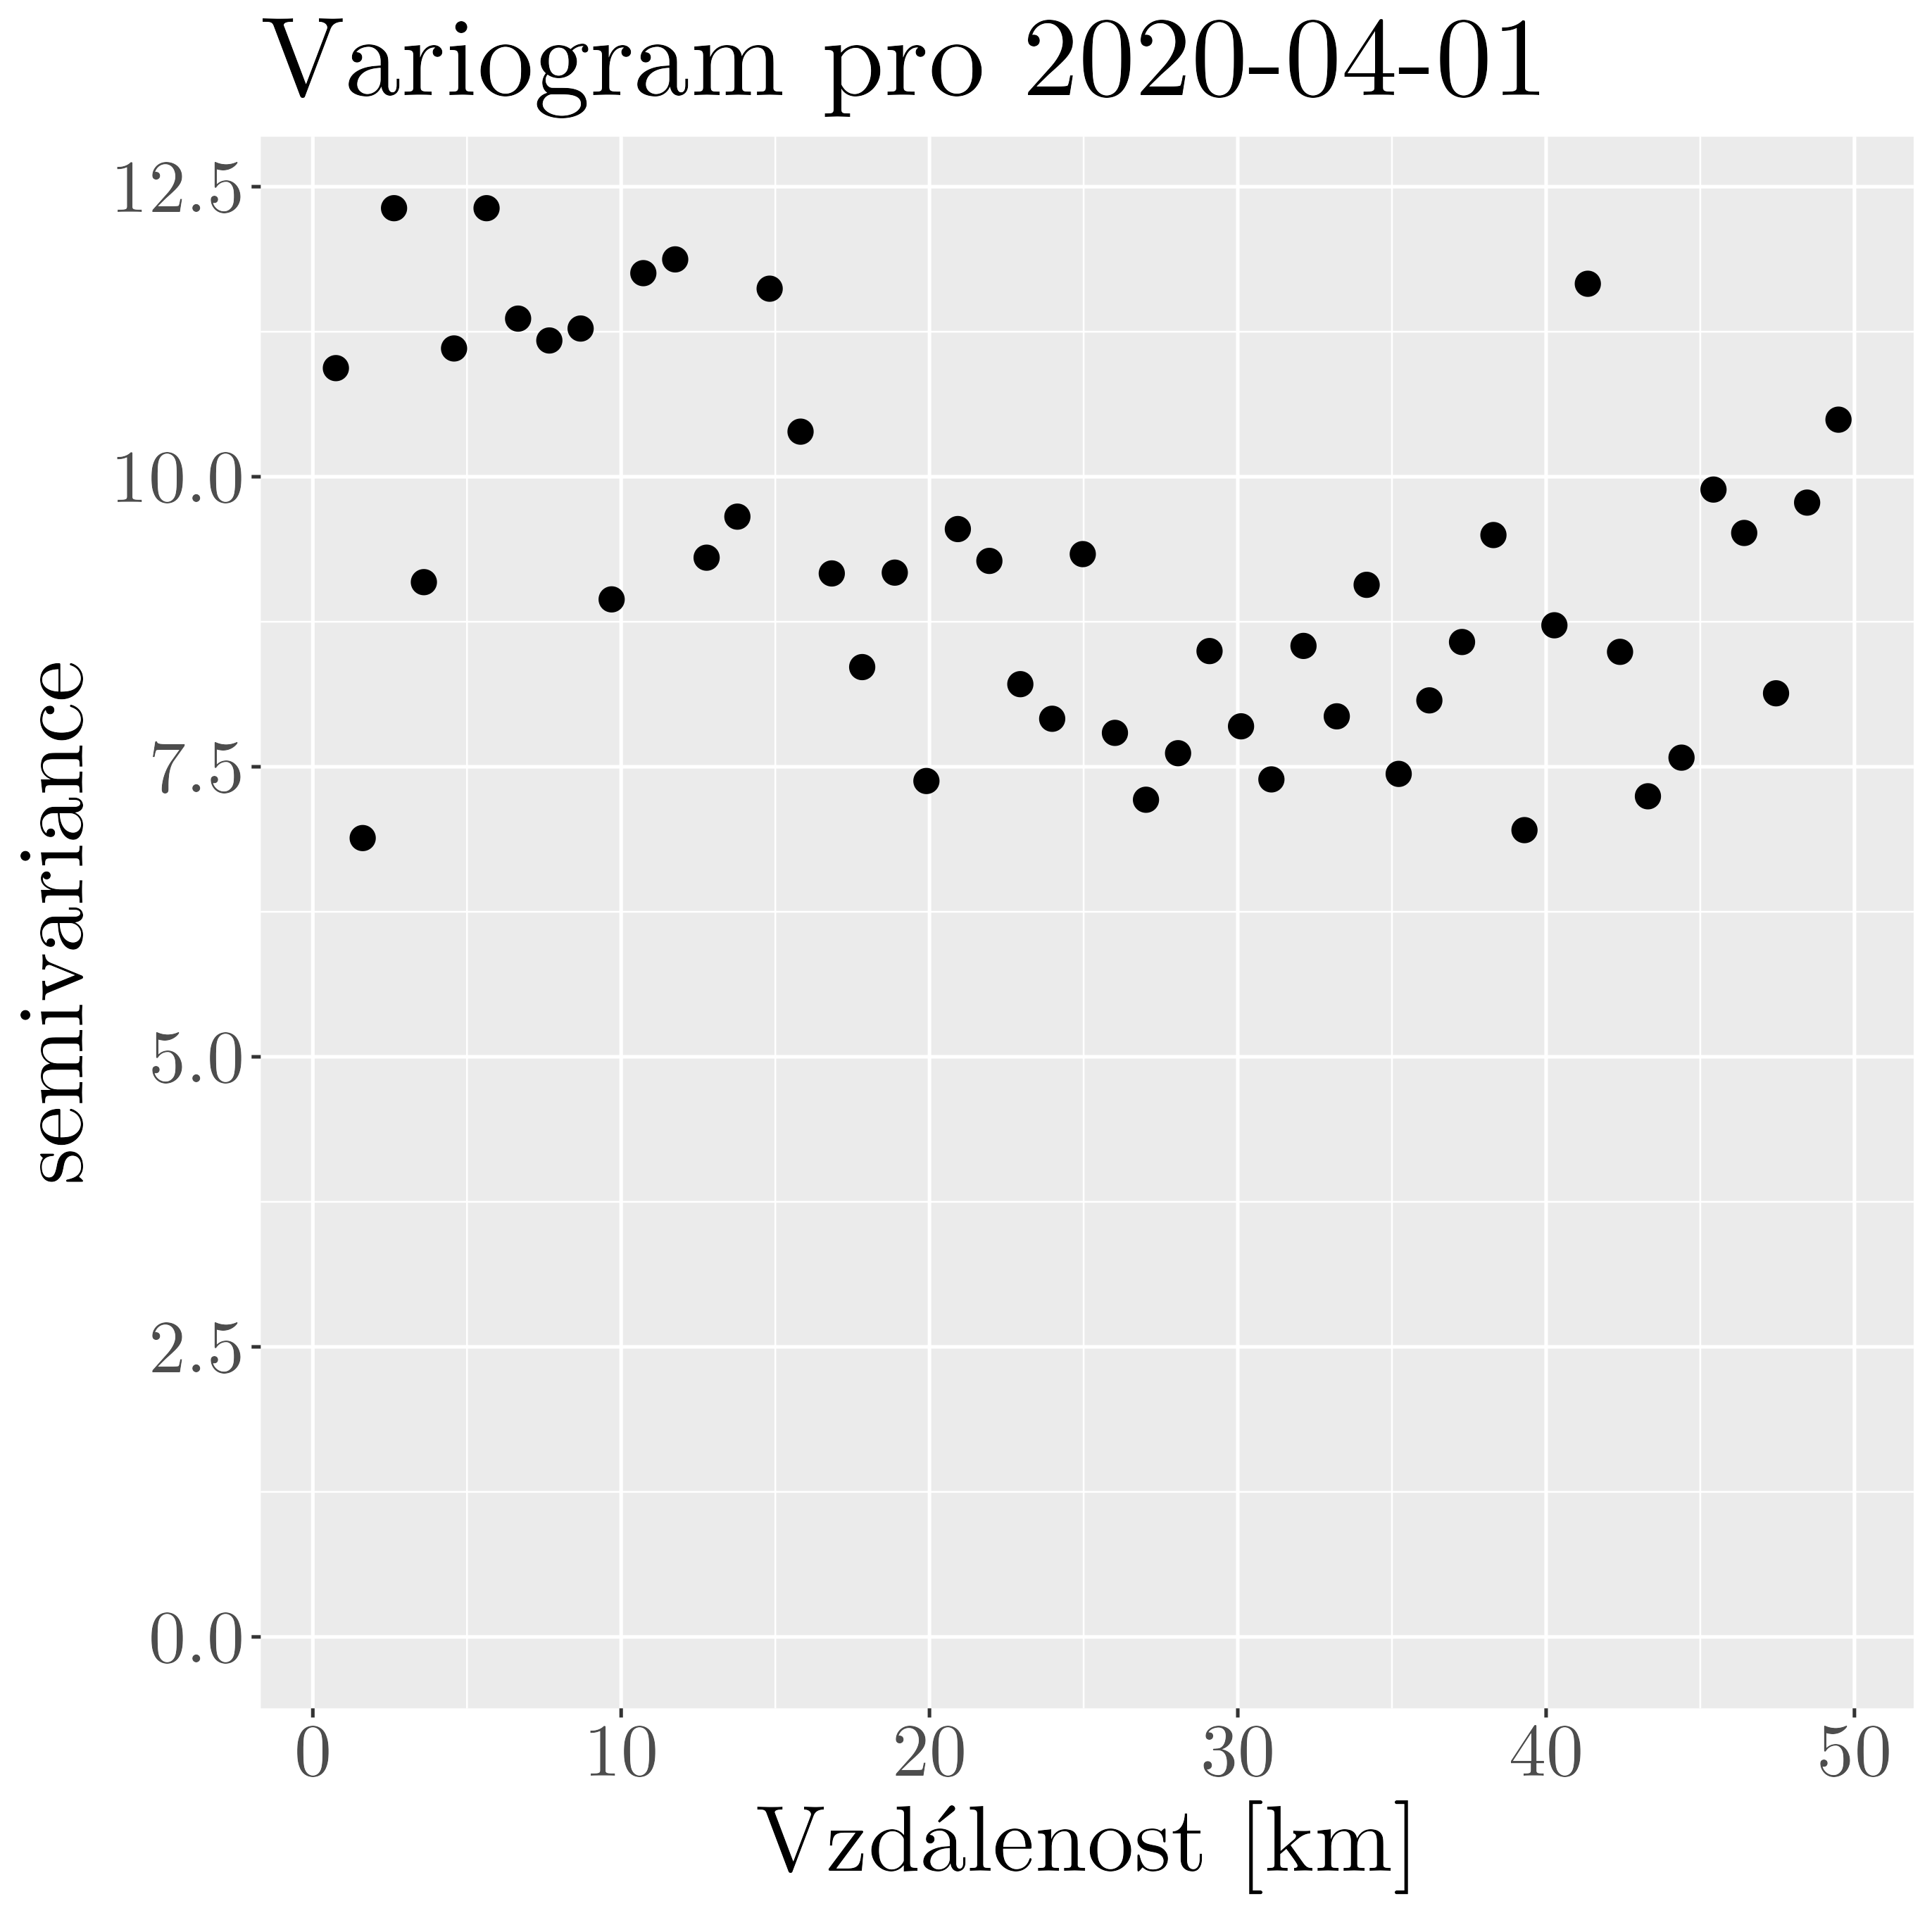
\includegraphics[width=\textwidth]{img/ch2/variograms/variogram_max15cm4.png}
		\caption{}
		\label{fig:variogram4}
	\end{subfigure}
	\hfill
	\begin{subfigure}{0.30\textwidth}
		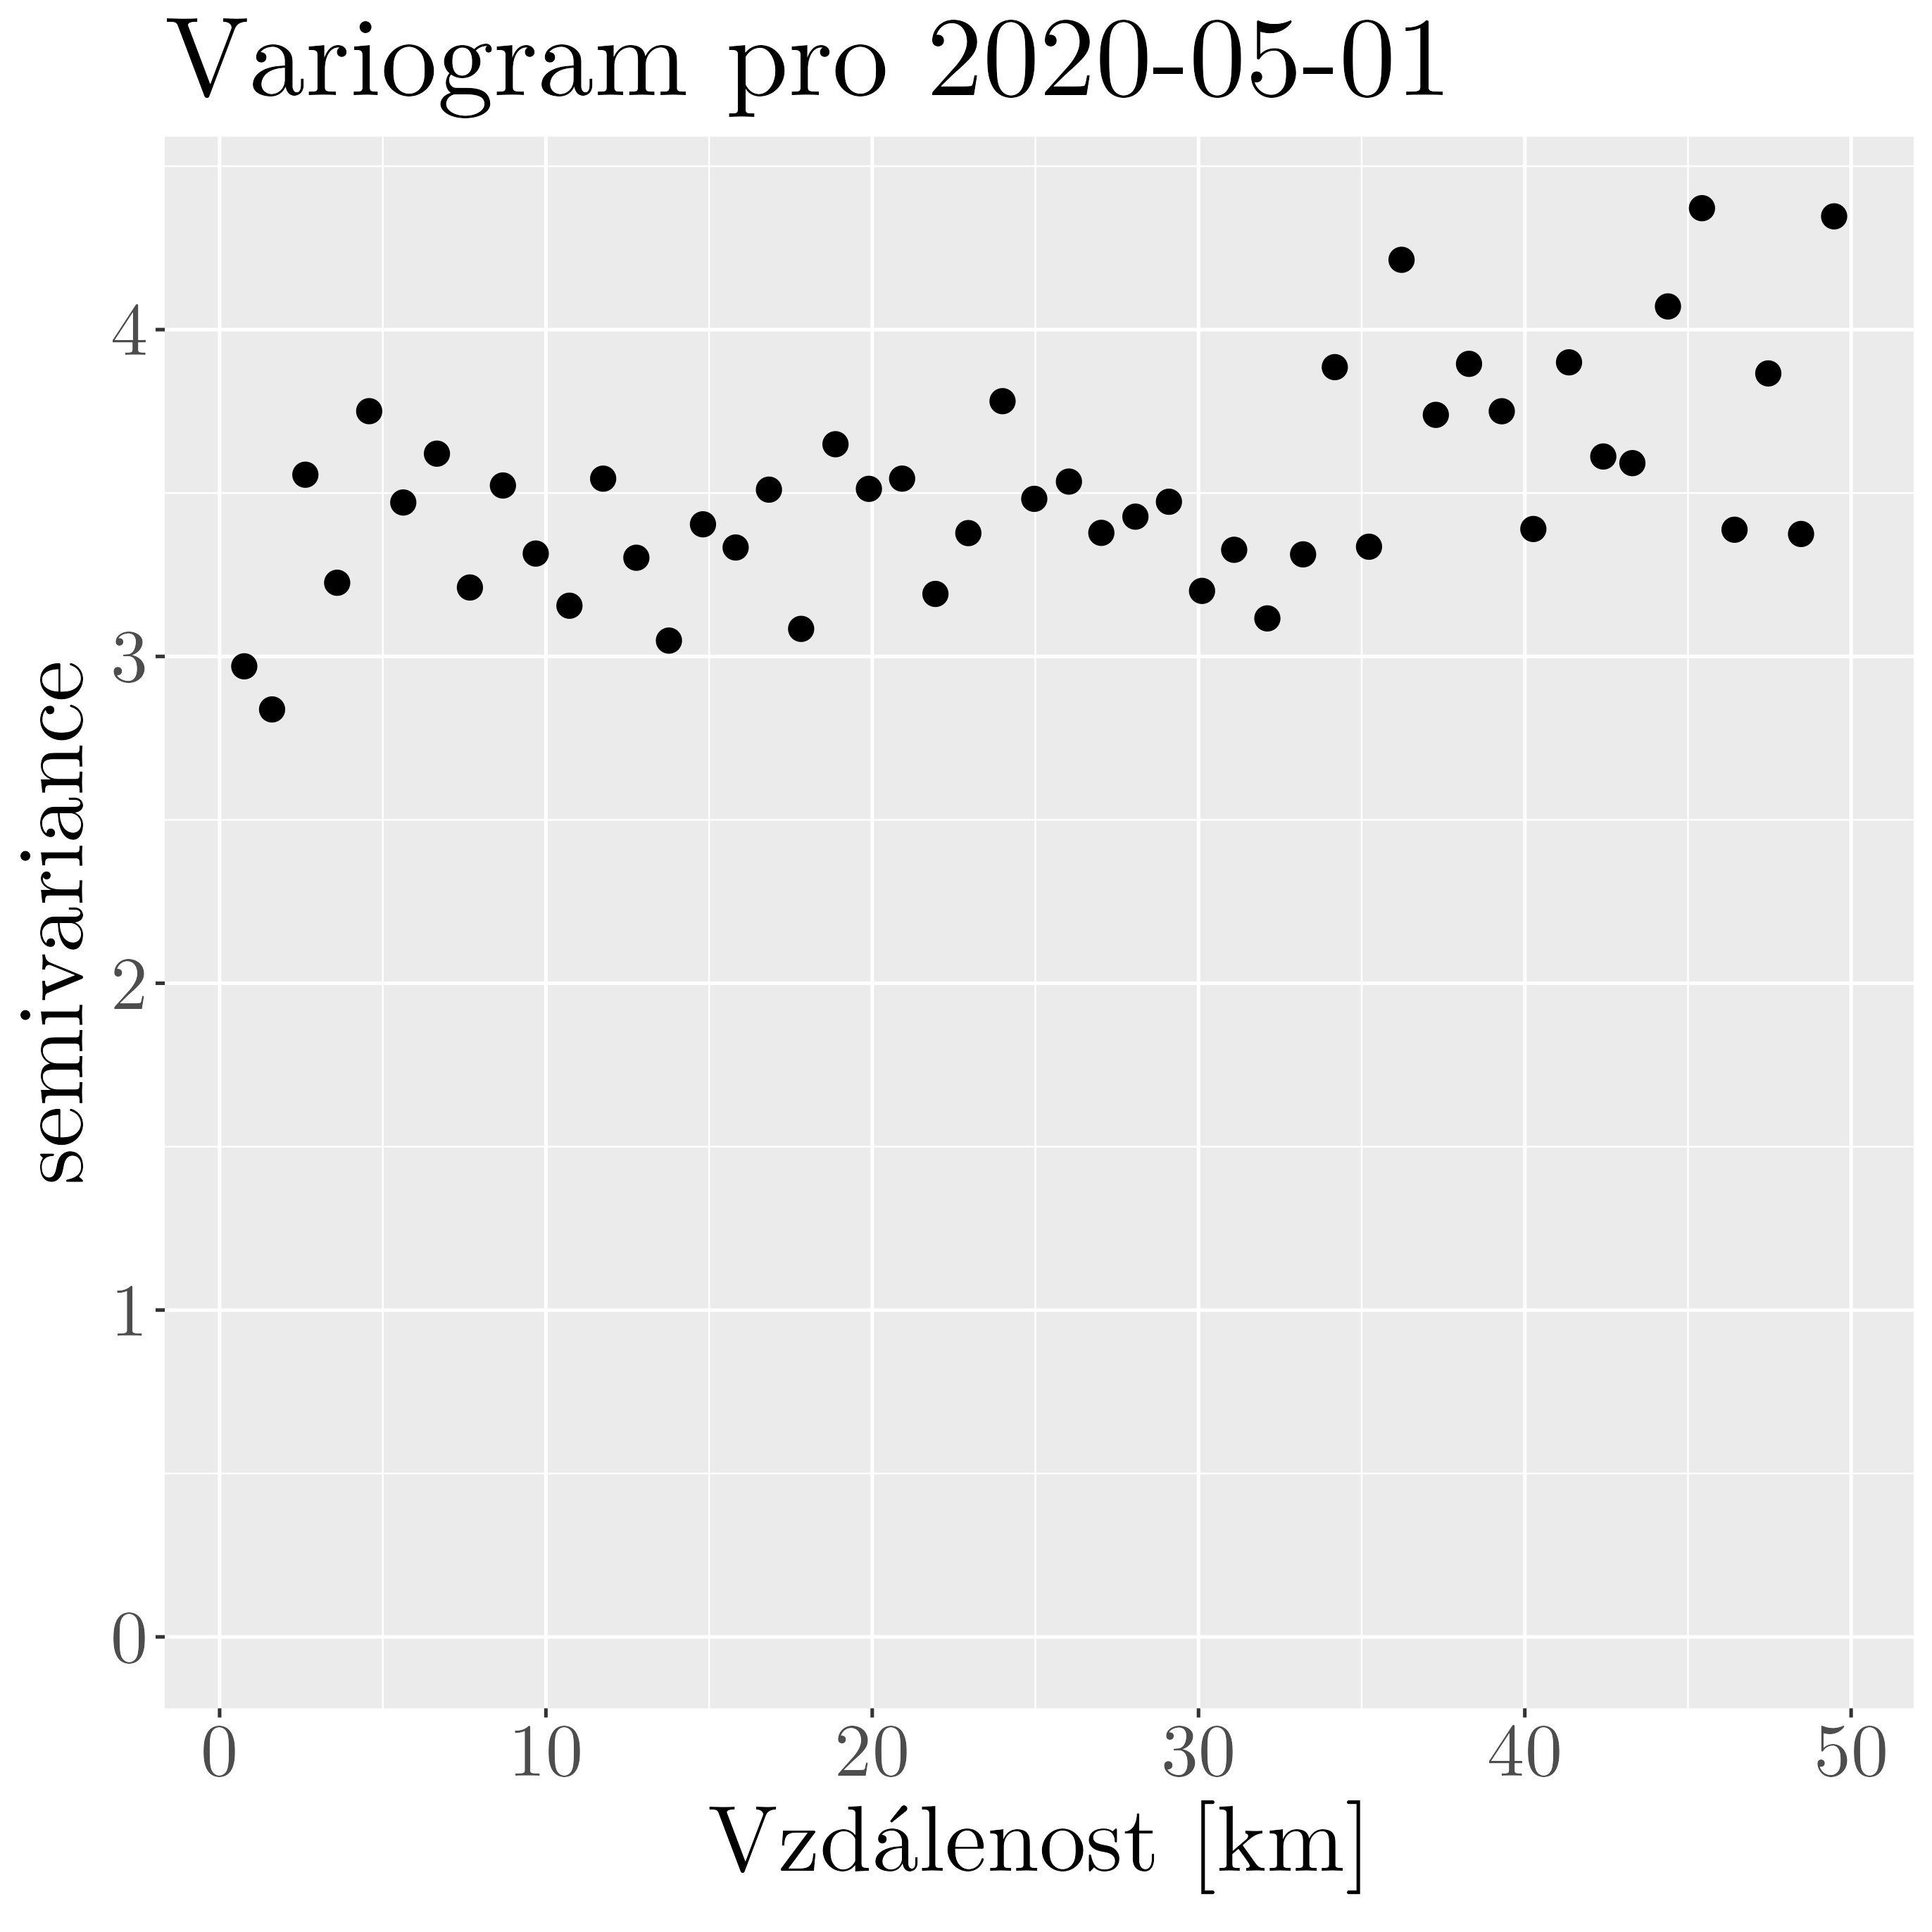
\includegraphics[width=\textwidth]{img/ch2/variograms/variogram_max15cm5.png}
		\caption{}
		\label{fig:variogram5}
	\end{subfigure}
	\hfill
	\begin{subfigure}{0.30\textwidth}
		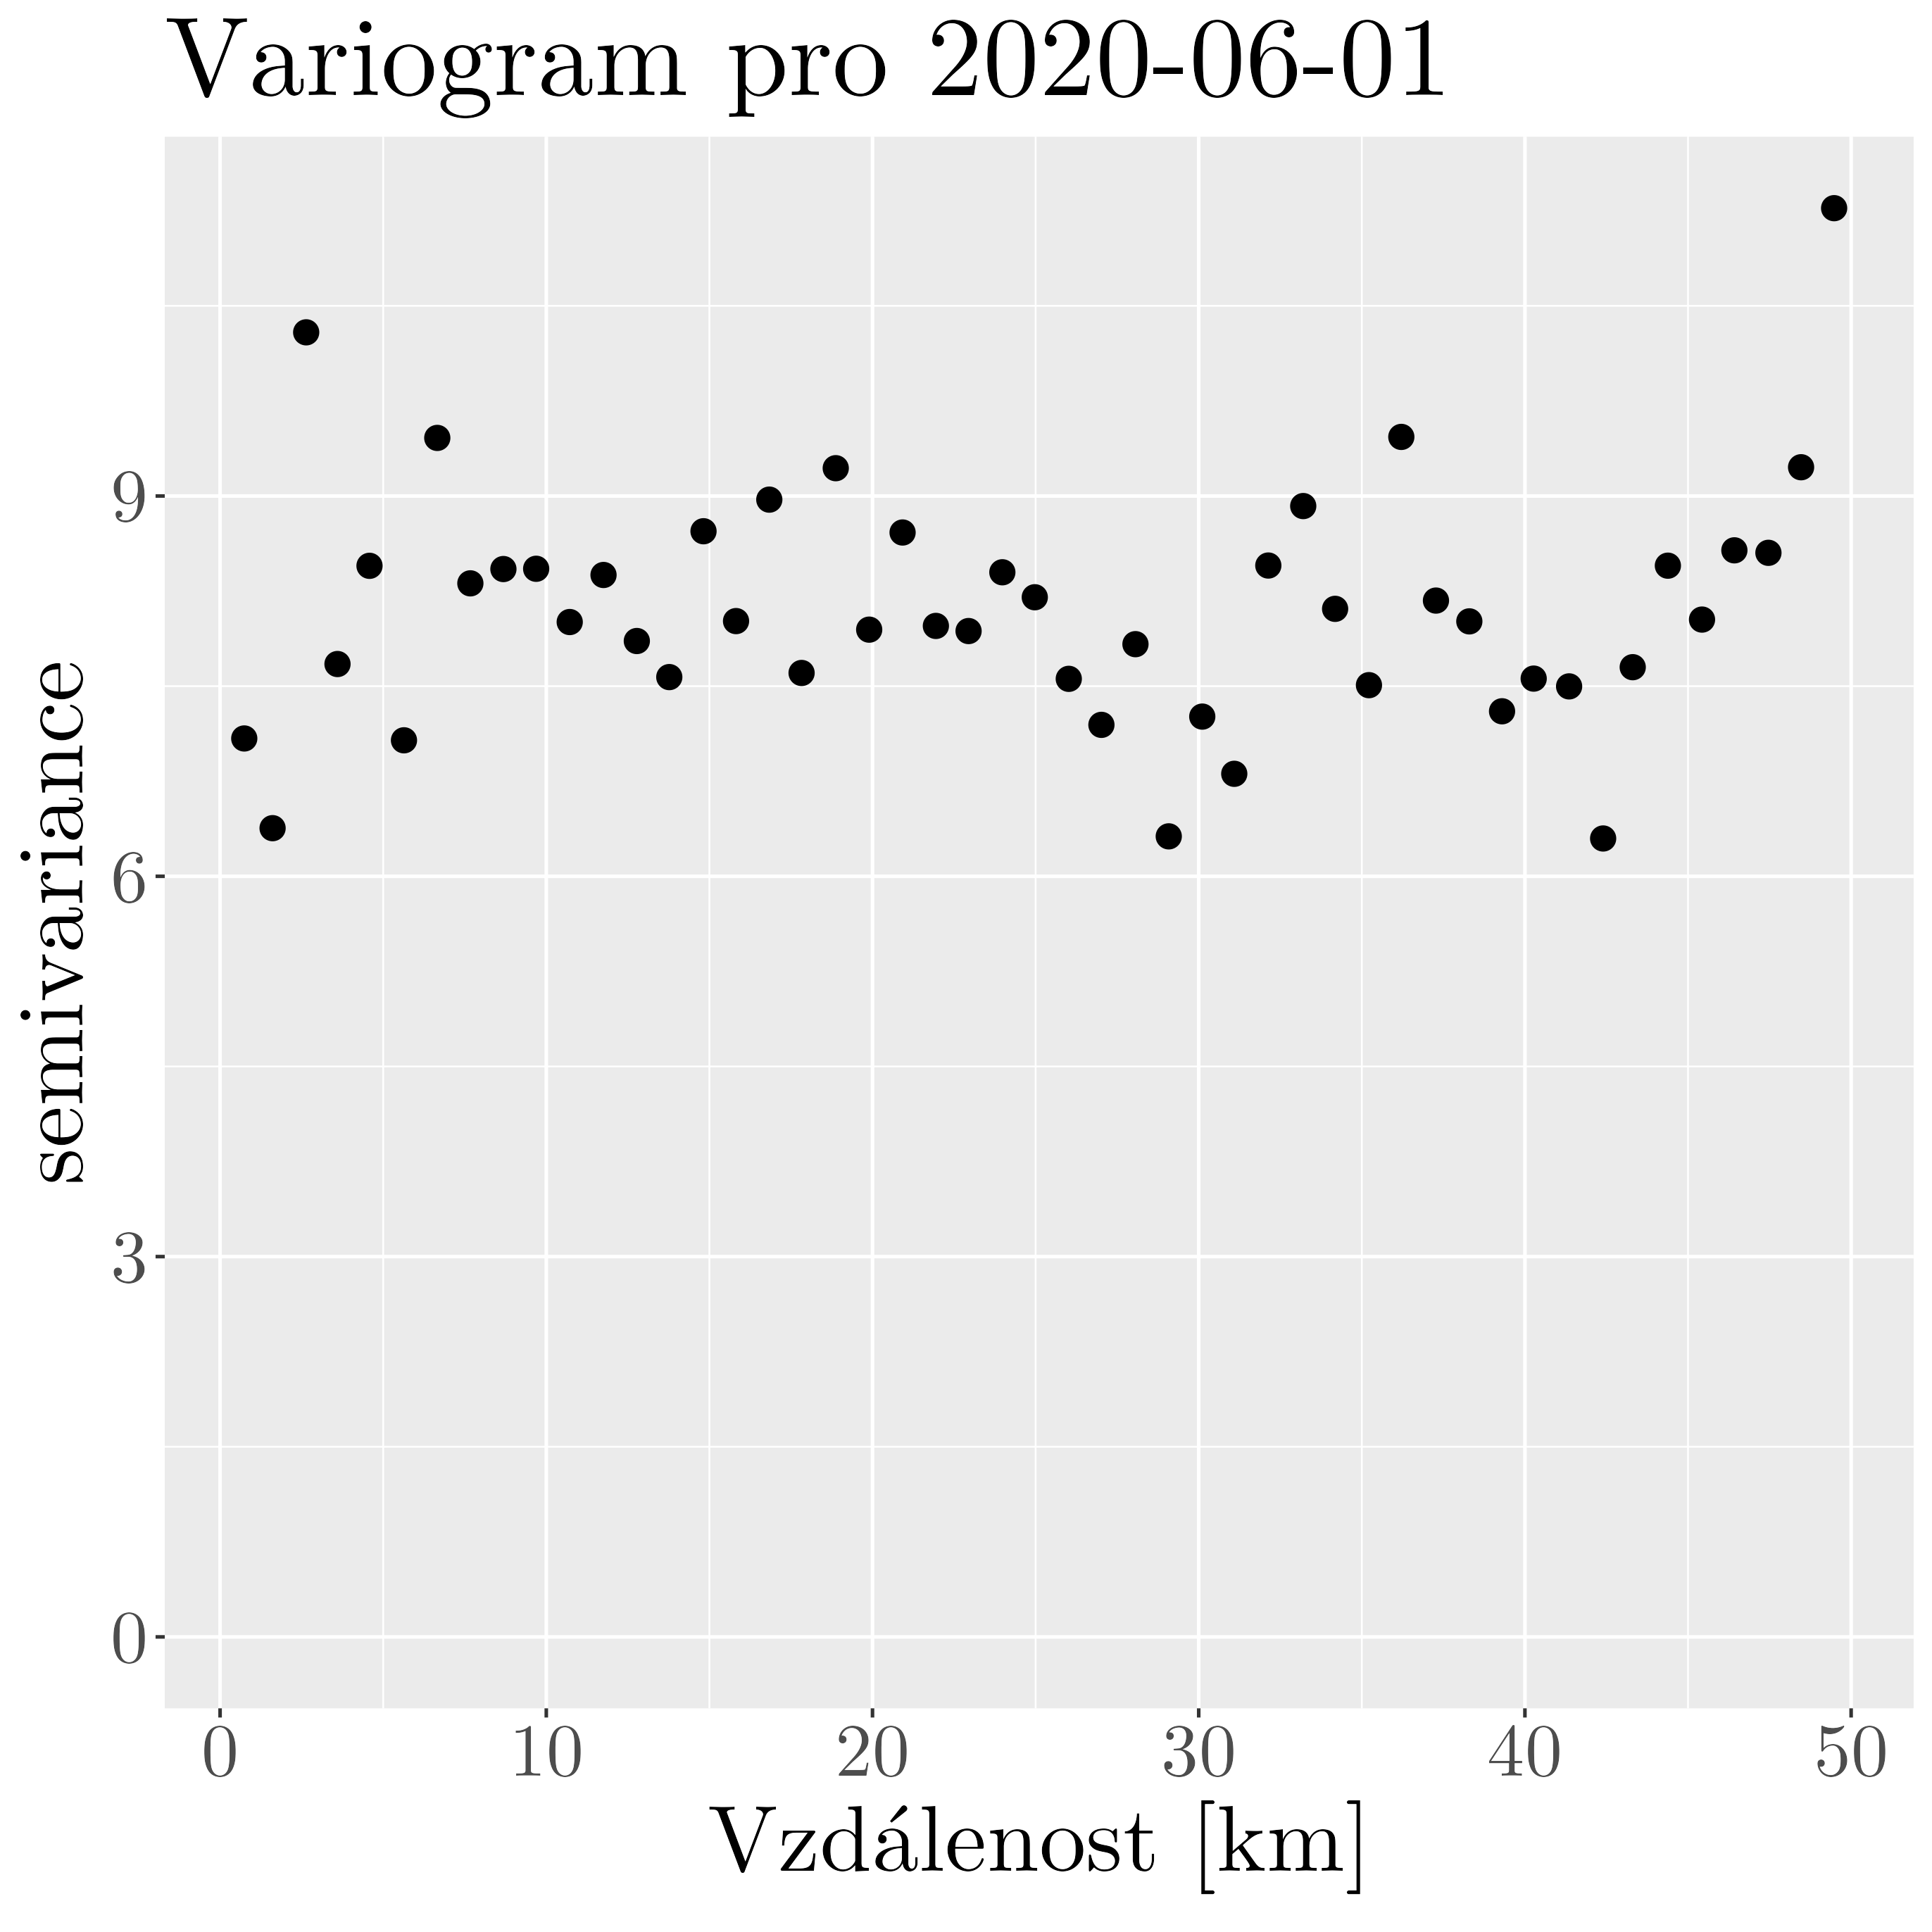
\includegraphics[width=\textwidth]{img/ch2/variograms/variogram_max15cm6.png}
		\caption{}
		\label{fig:variogram6}
	\end{subfigure}
\hfill
	\begin{subfigure}{0.30\textwidth}
		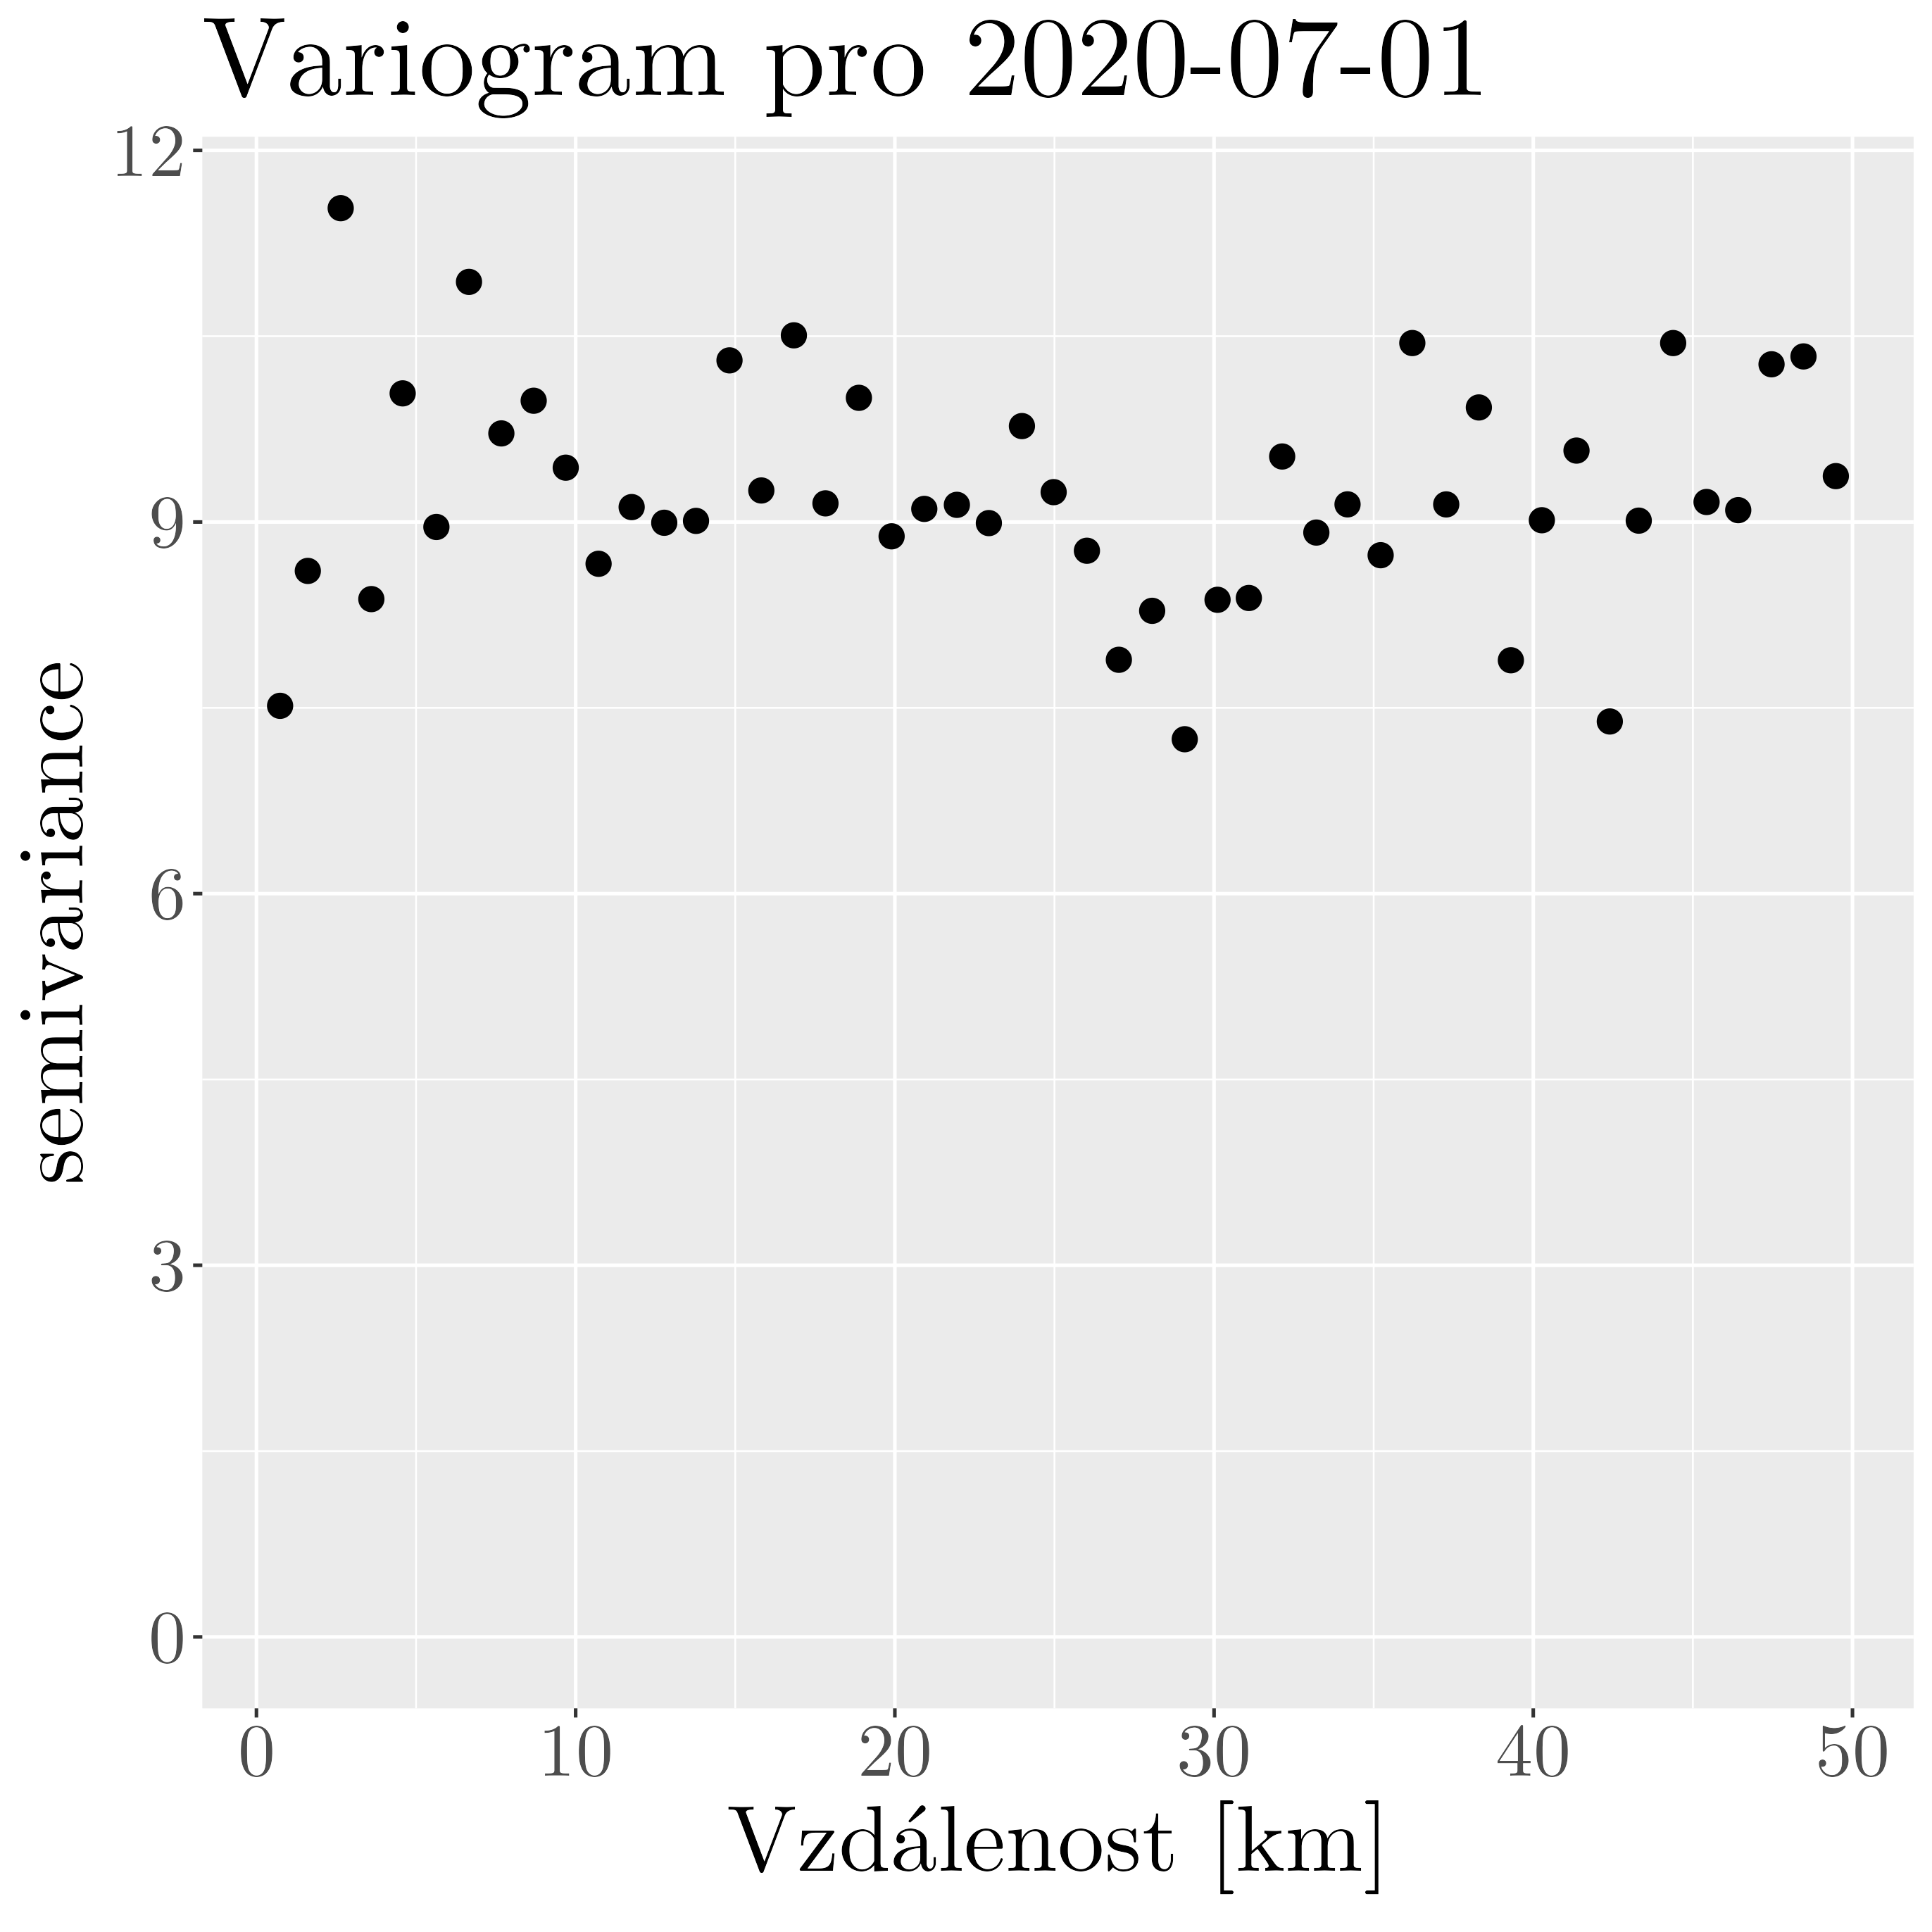
\includegraphics[width=\textwidth]{img/ch2/variograms/variogram_max15cm7.png}
		\caption{}
		\label{fig:variogram7}
	\end{subfigure}
\hfill
	\begin{subfigure}{0.30\textwidth}
		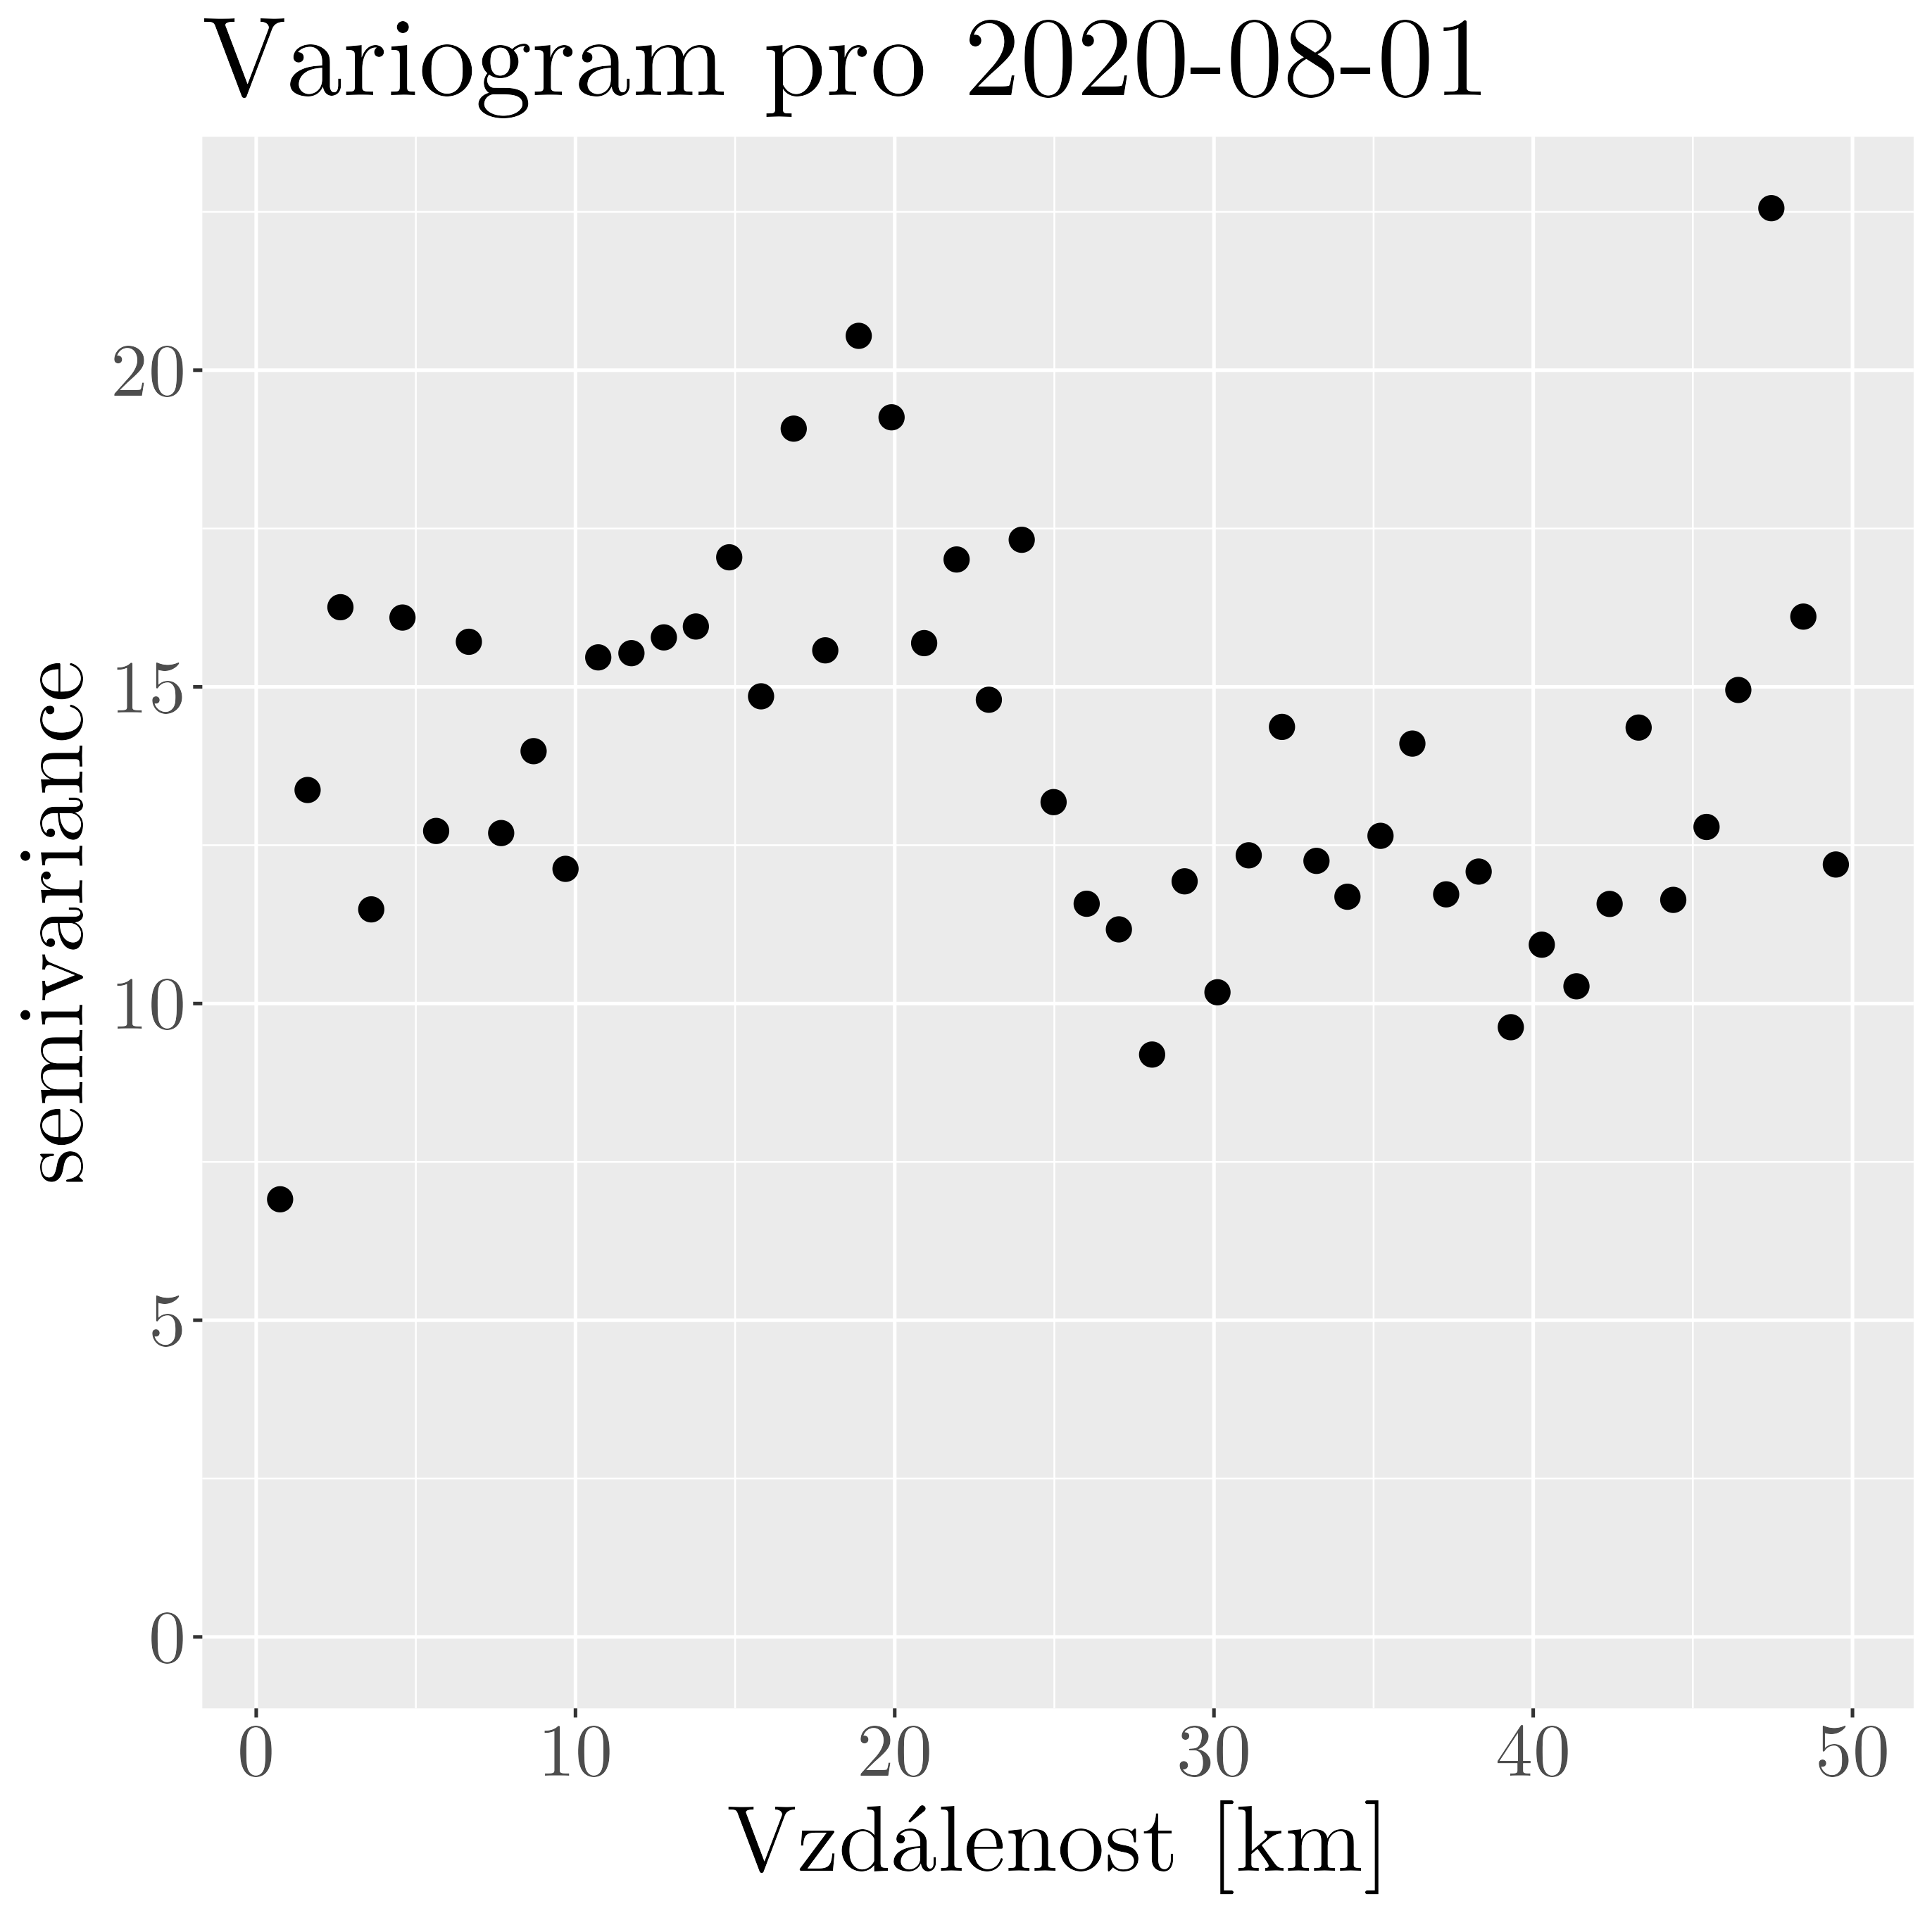
\includegraphics[width=\textwidth]{img/ch2/variograms/variogram_max15cm8.png}
		\caption{}
		\label{fig:variogram8}
	\end{subfigure}
\hfill
	\begin{subfigure}{0.30\textwidth}
		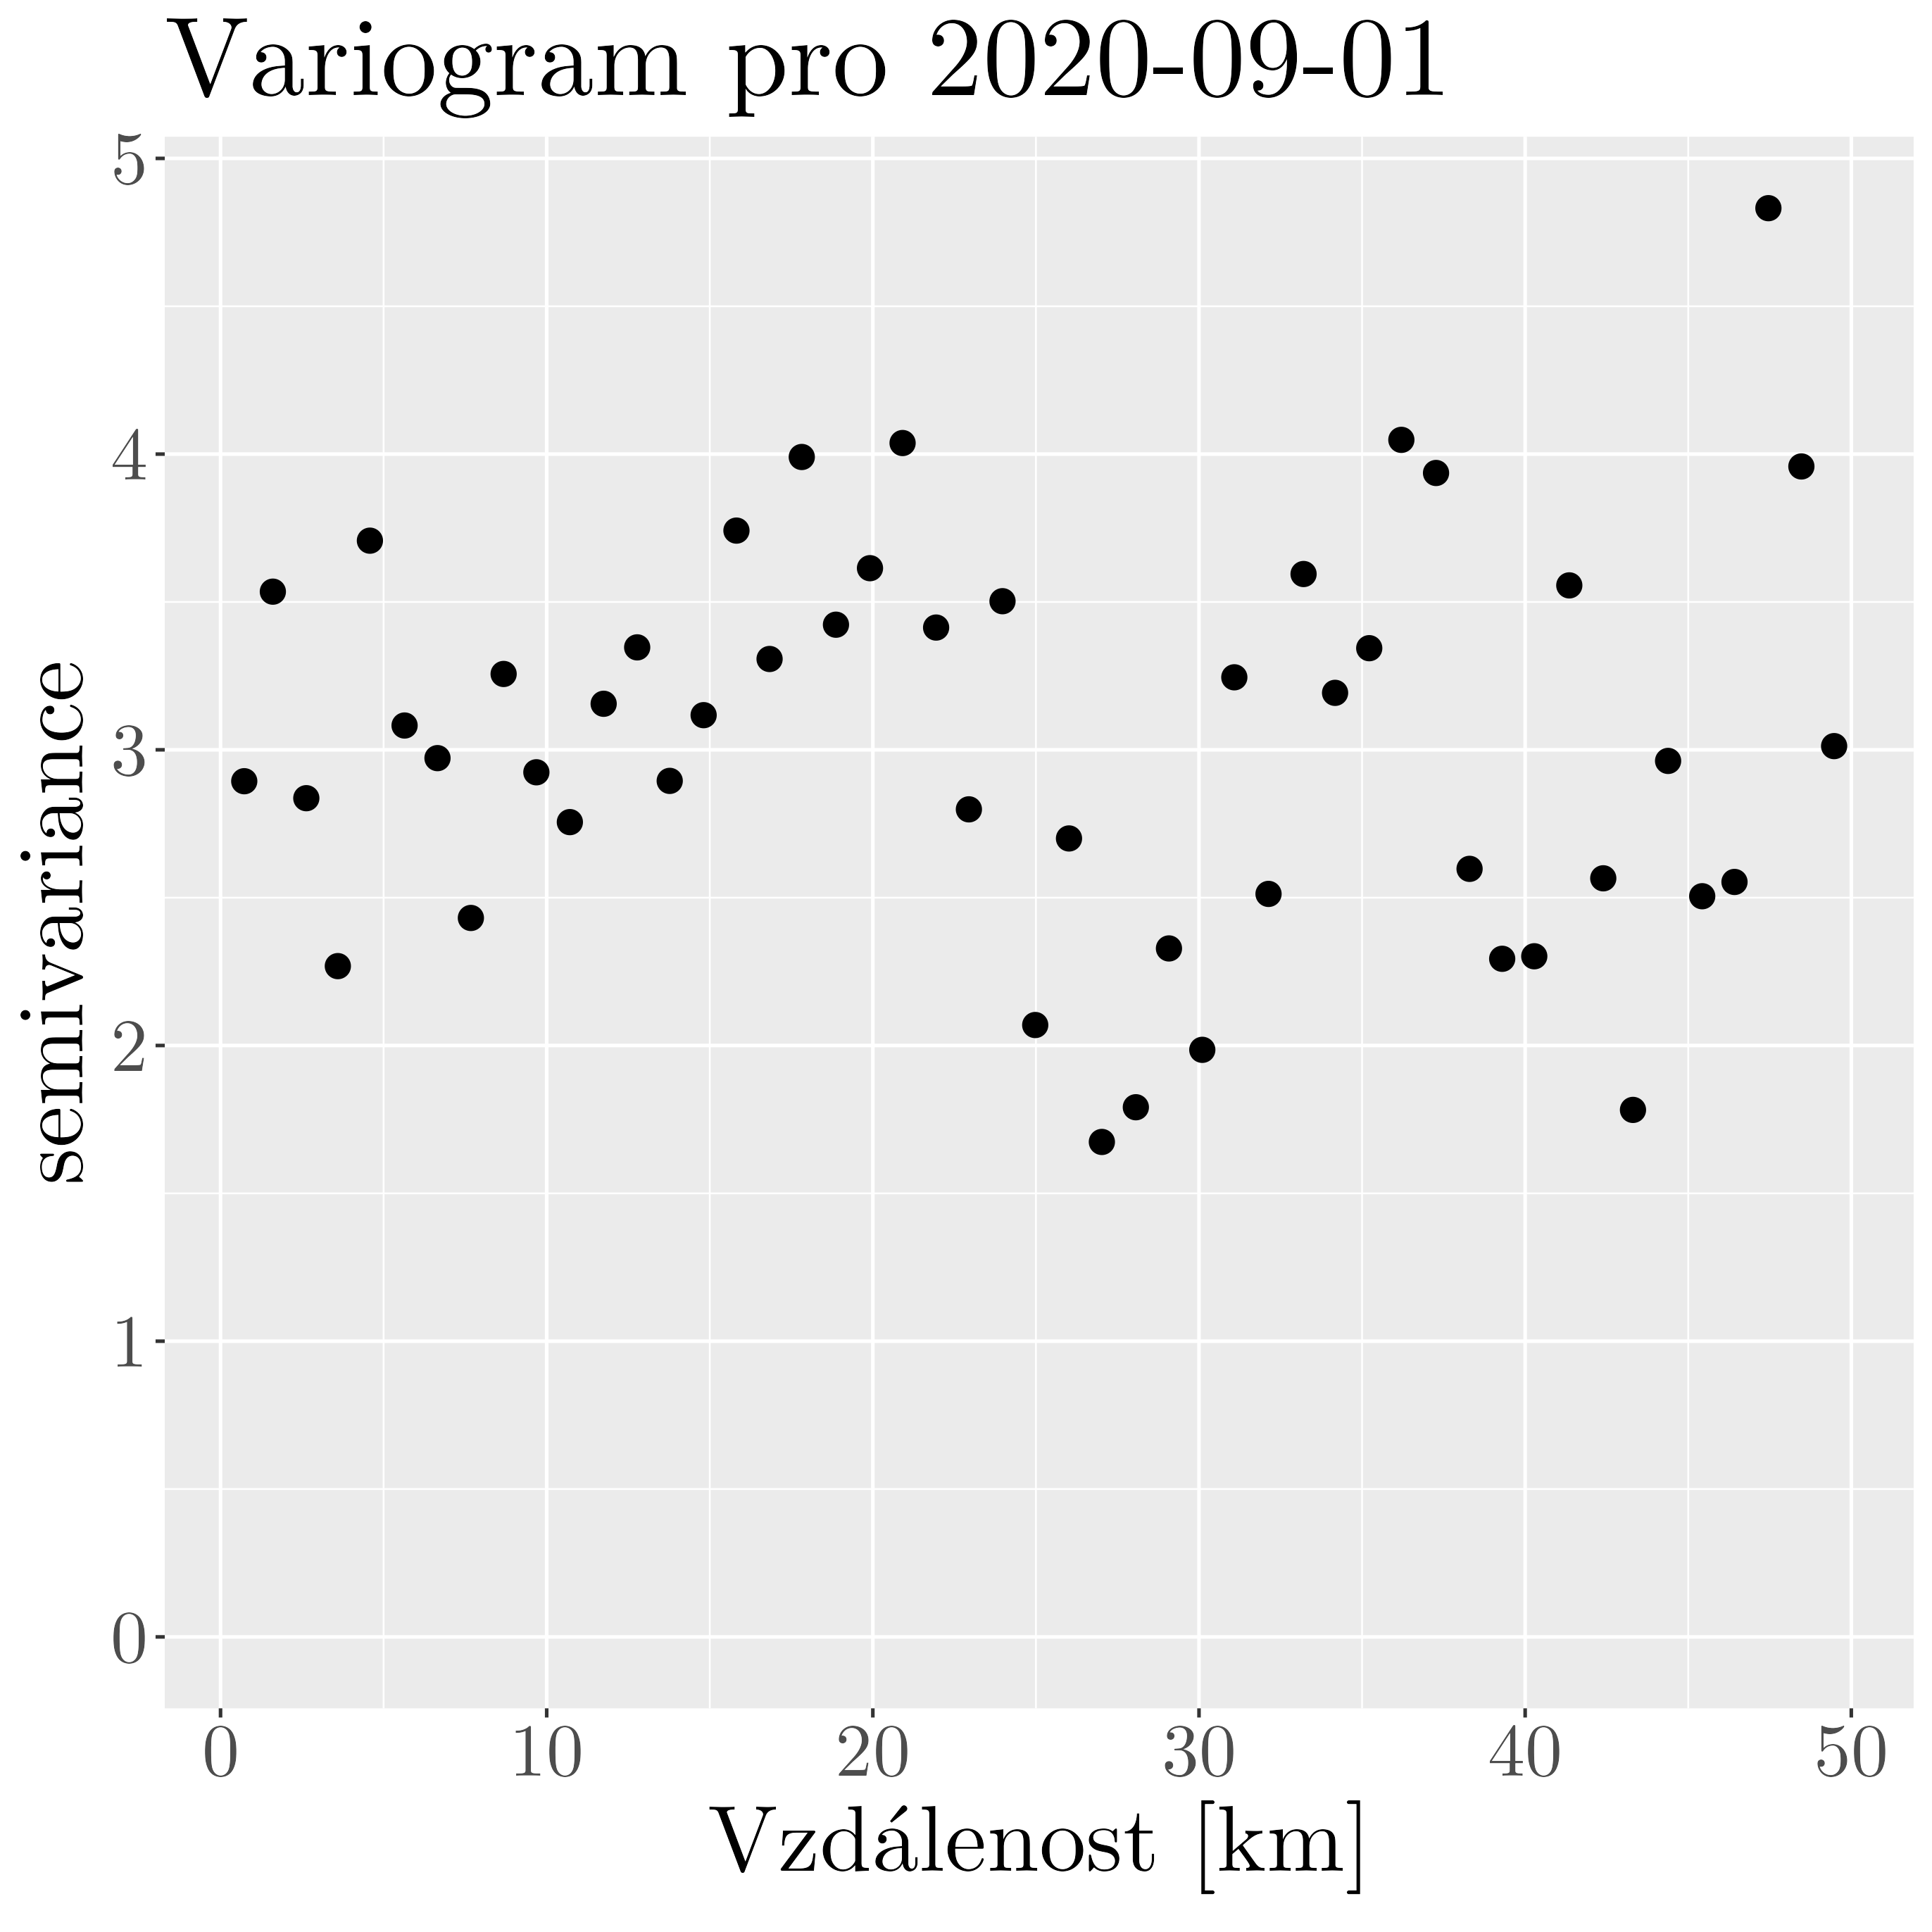
\includegraphics[width=\textwidth]{img/ch2/variograms/variogram_max15cm9.png}
		\caption{}
		\label{fig:variogram9}
	\end{subfigure}
\hfill
	\begin{subfigure}{0.30\textwidth}
		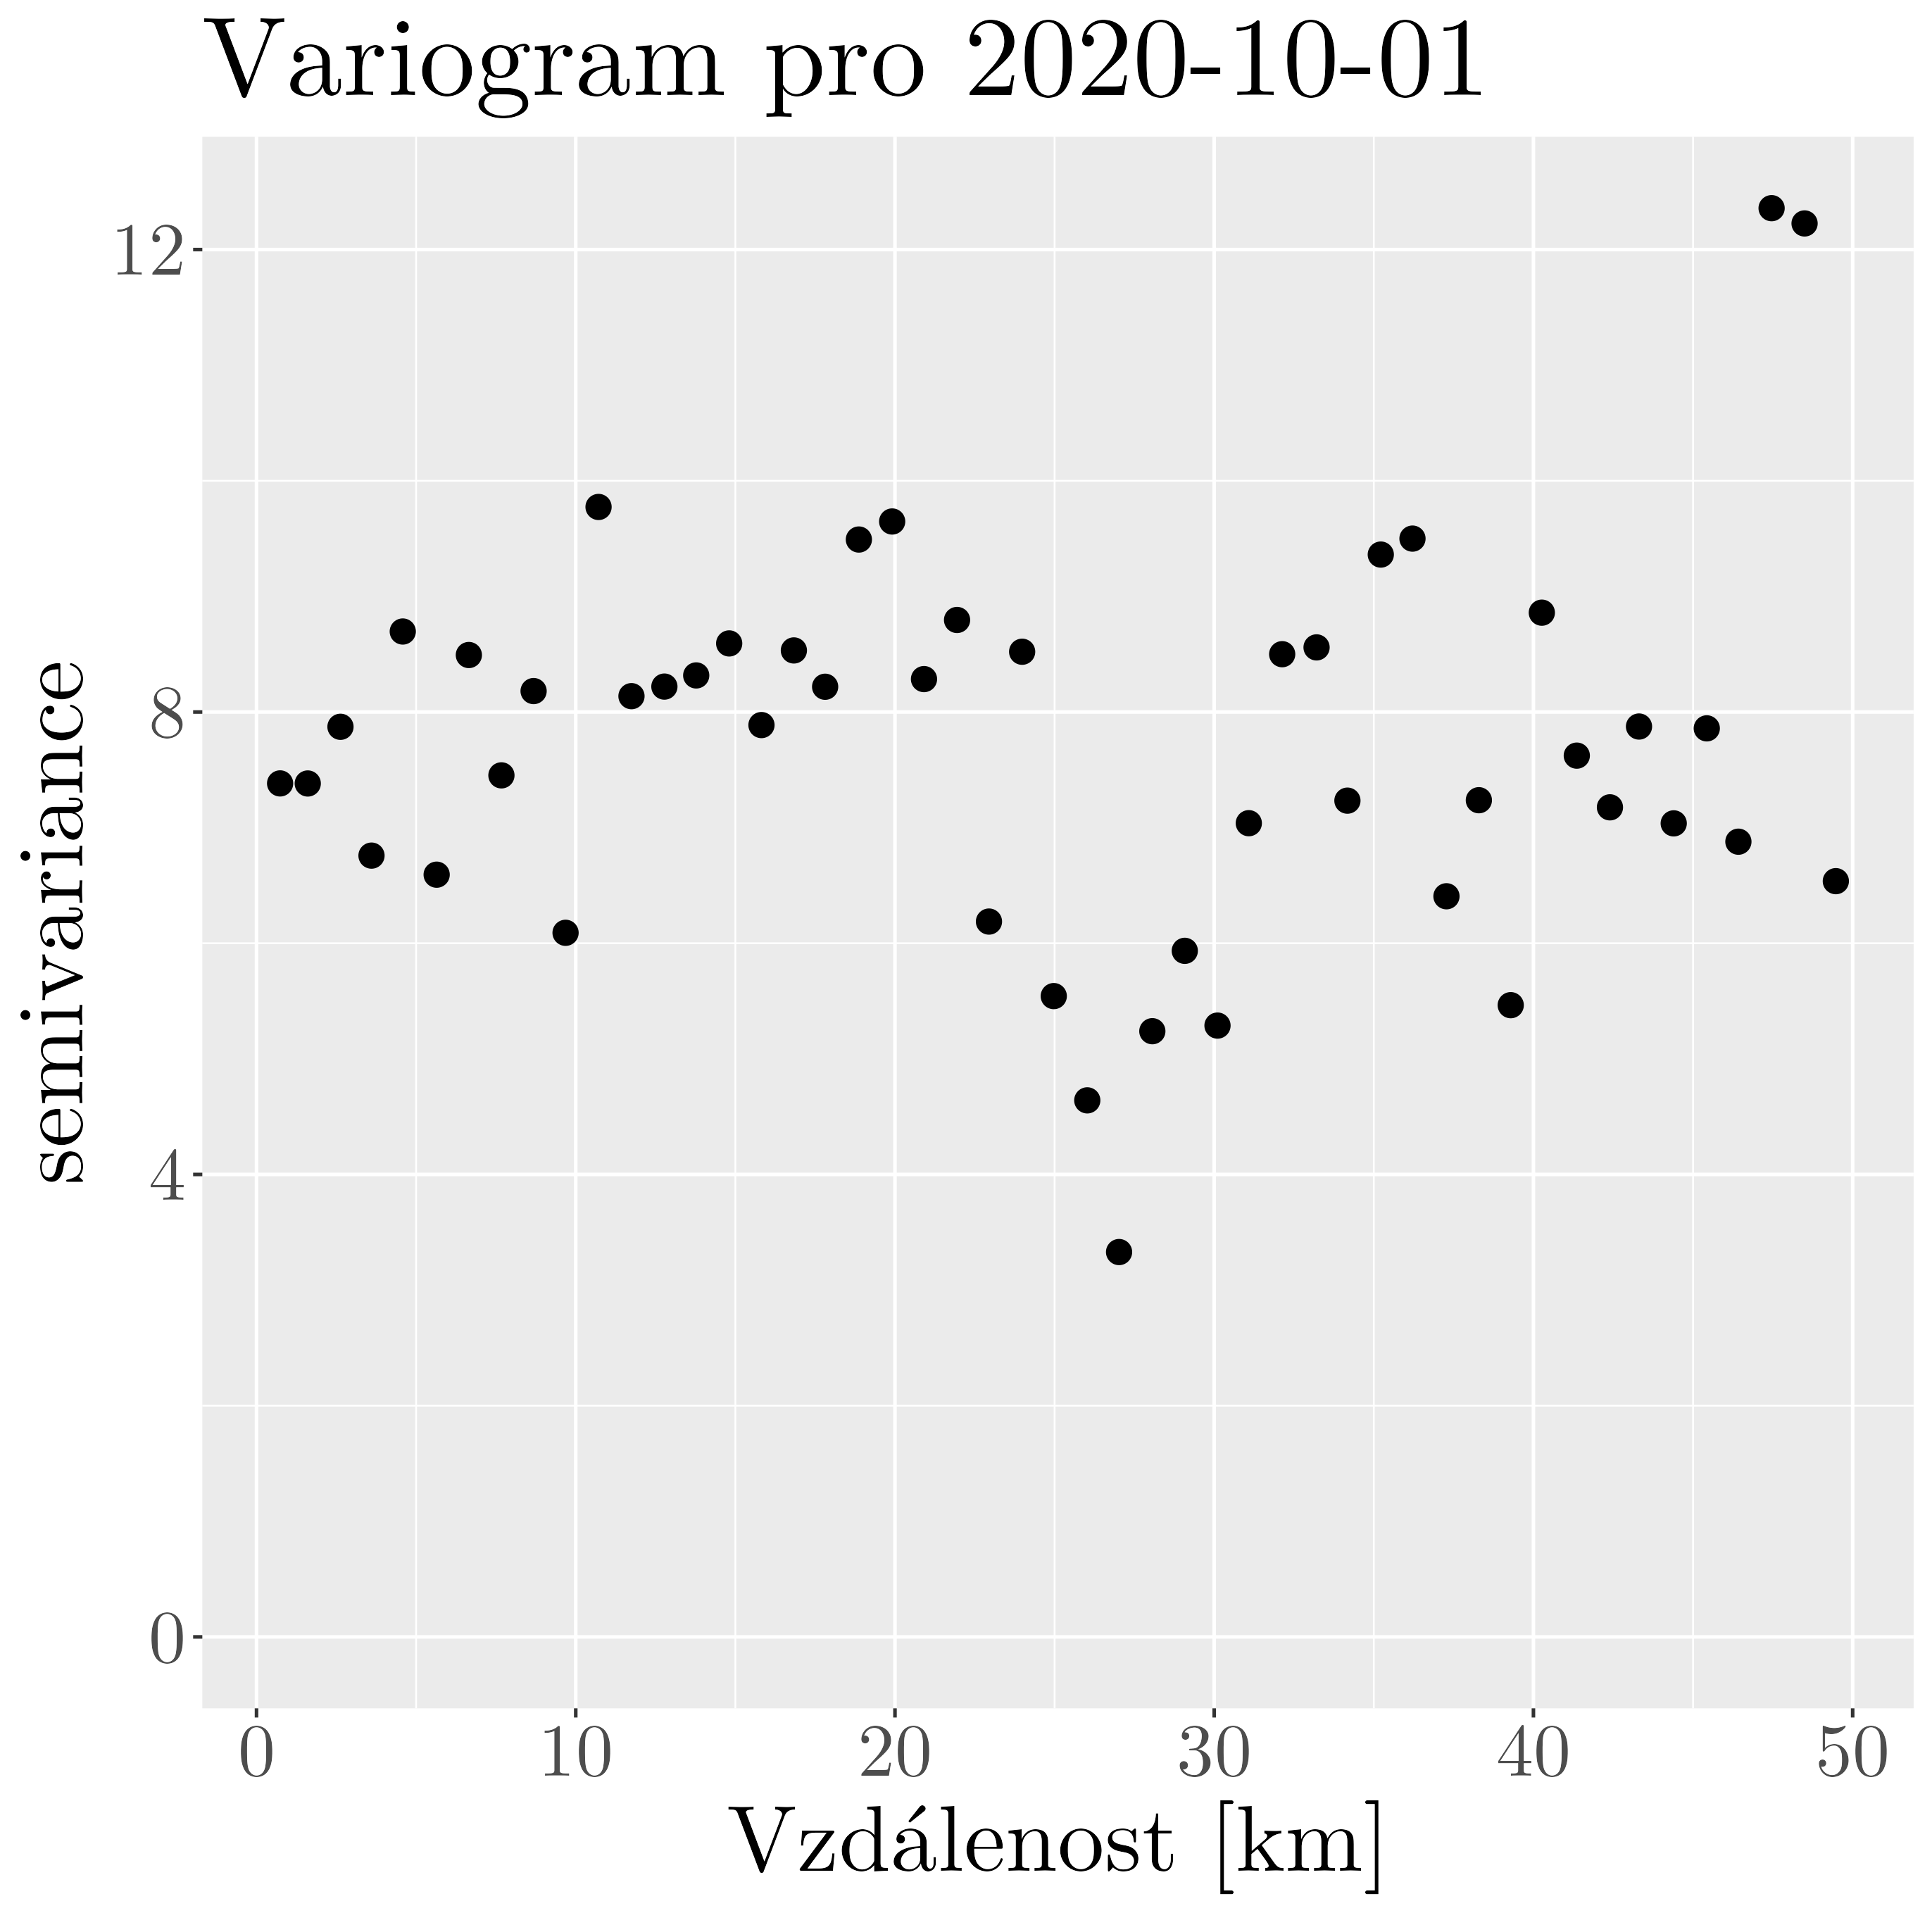
\includegraphics[width=\textwidth]{img/ch2/variograms/variogram_max15cm10.png}
		\caption{}
		\label{fig:variogram10}
	\end{subfigure}
\hfill
	\begin{subfigure}{0.30\textwidth}
		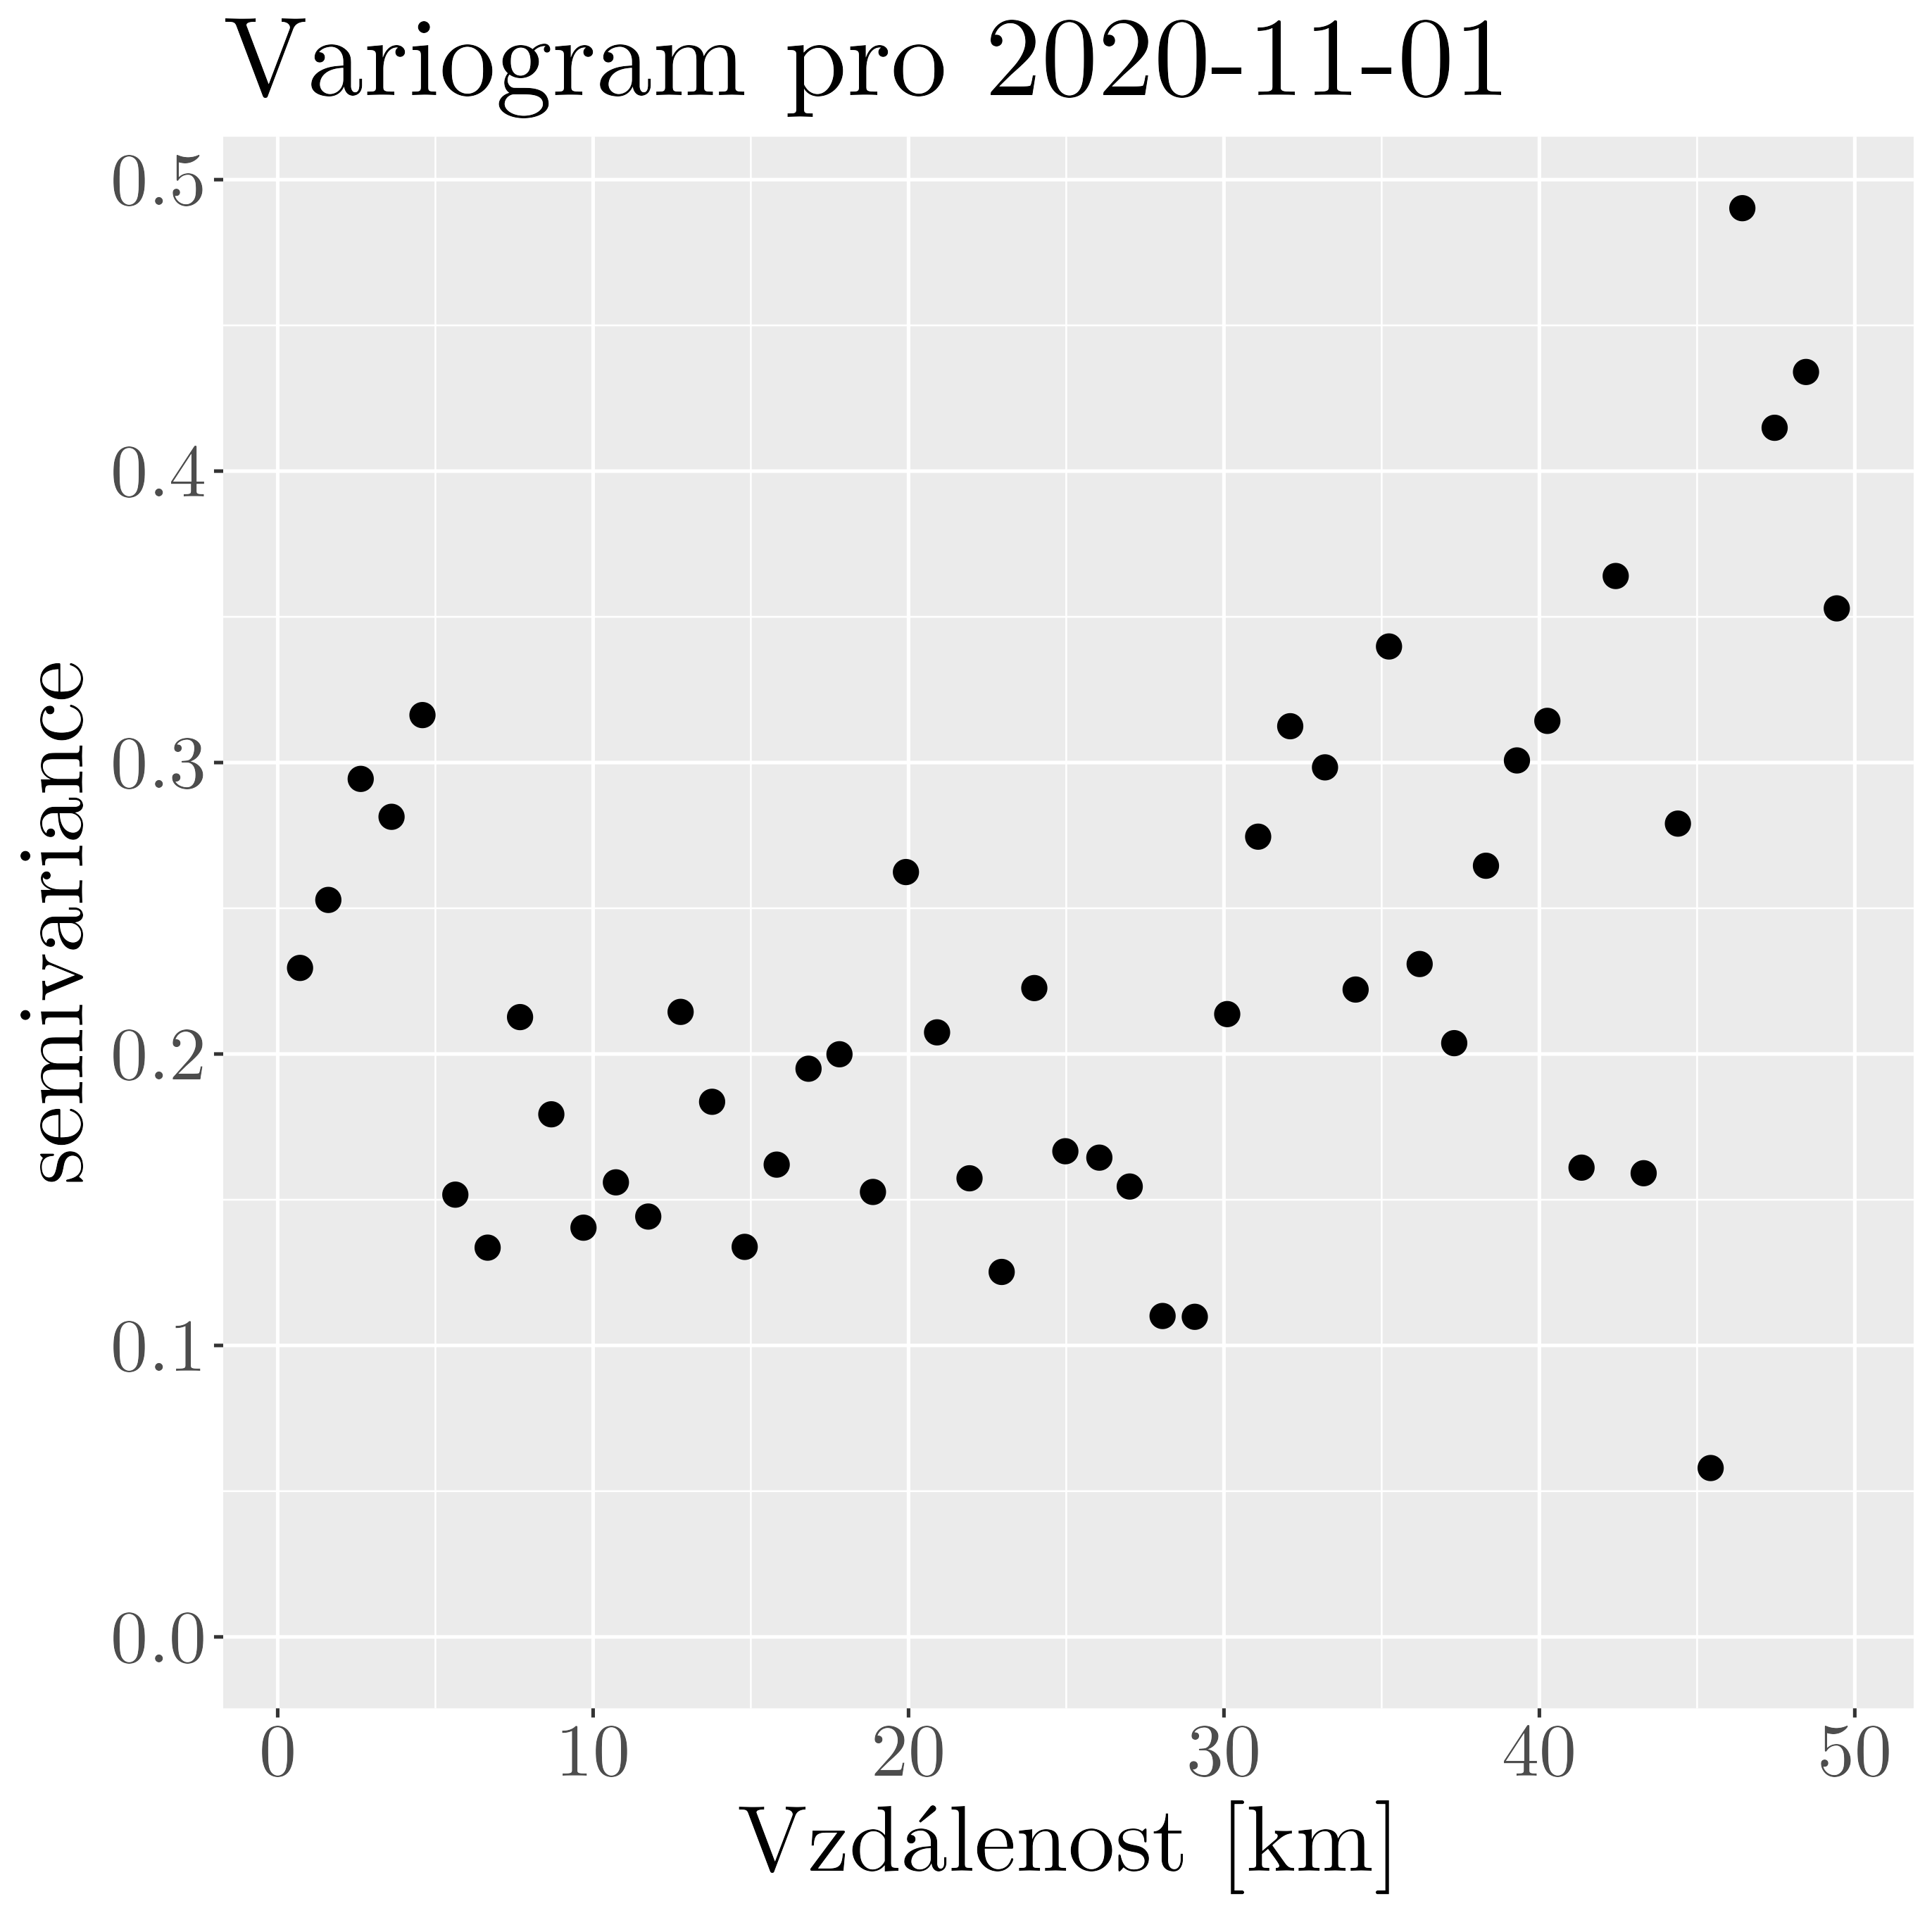
\includegraphics[width=\textwidth]{img/ch2/variograms/variogram_max15cm11.png}
		\caption{}
		\label{fig:variogram11}
	\end{subfigure}
\hfill
	\begin{subfigure}{0.30\textwidth}
		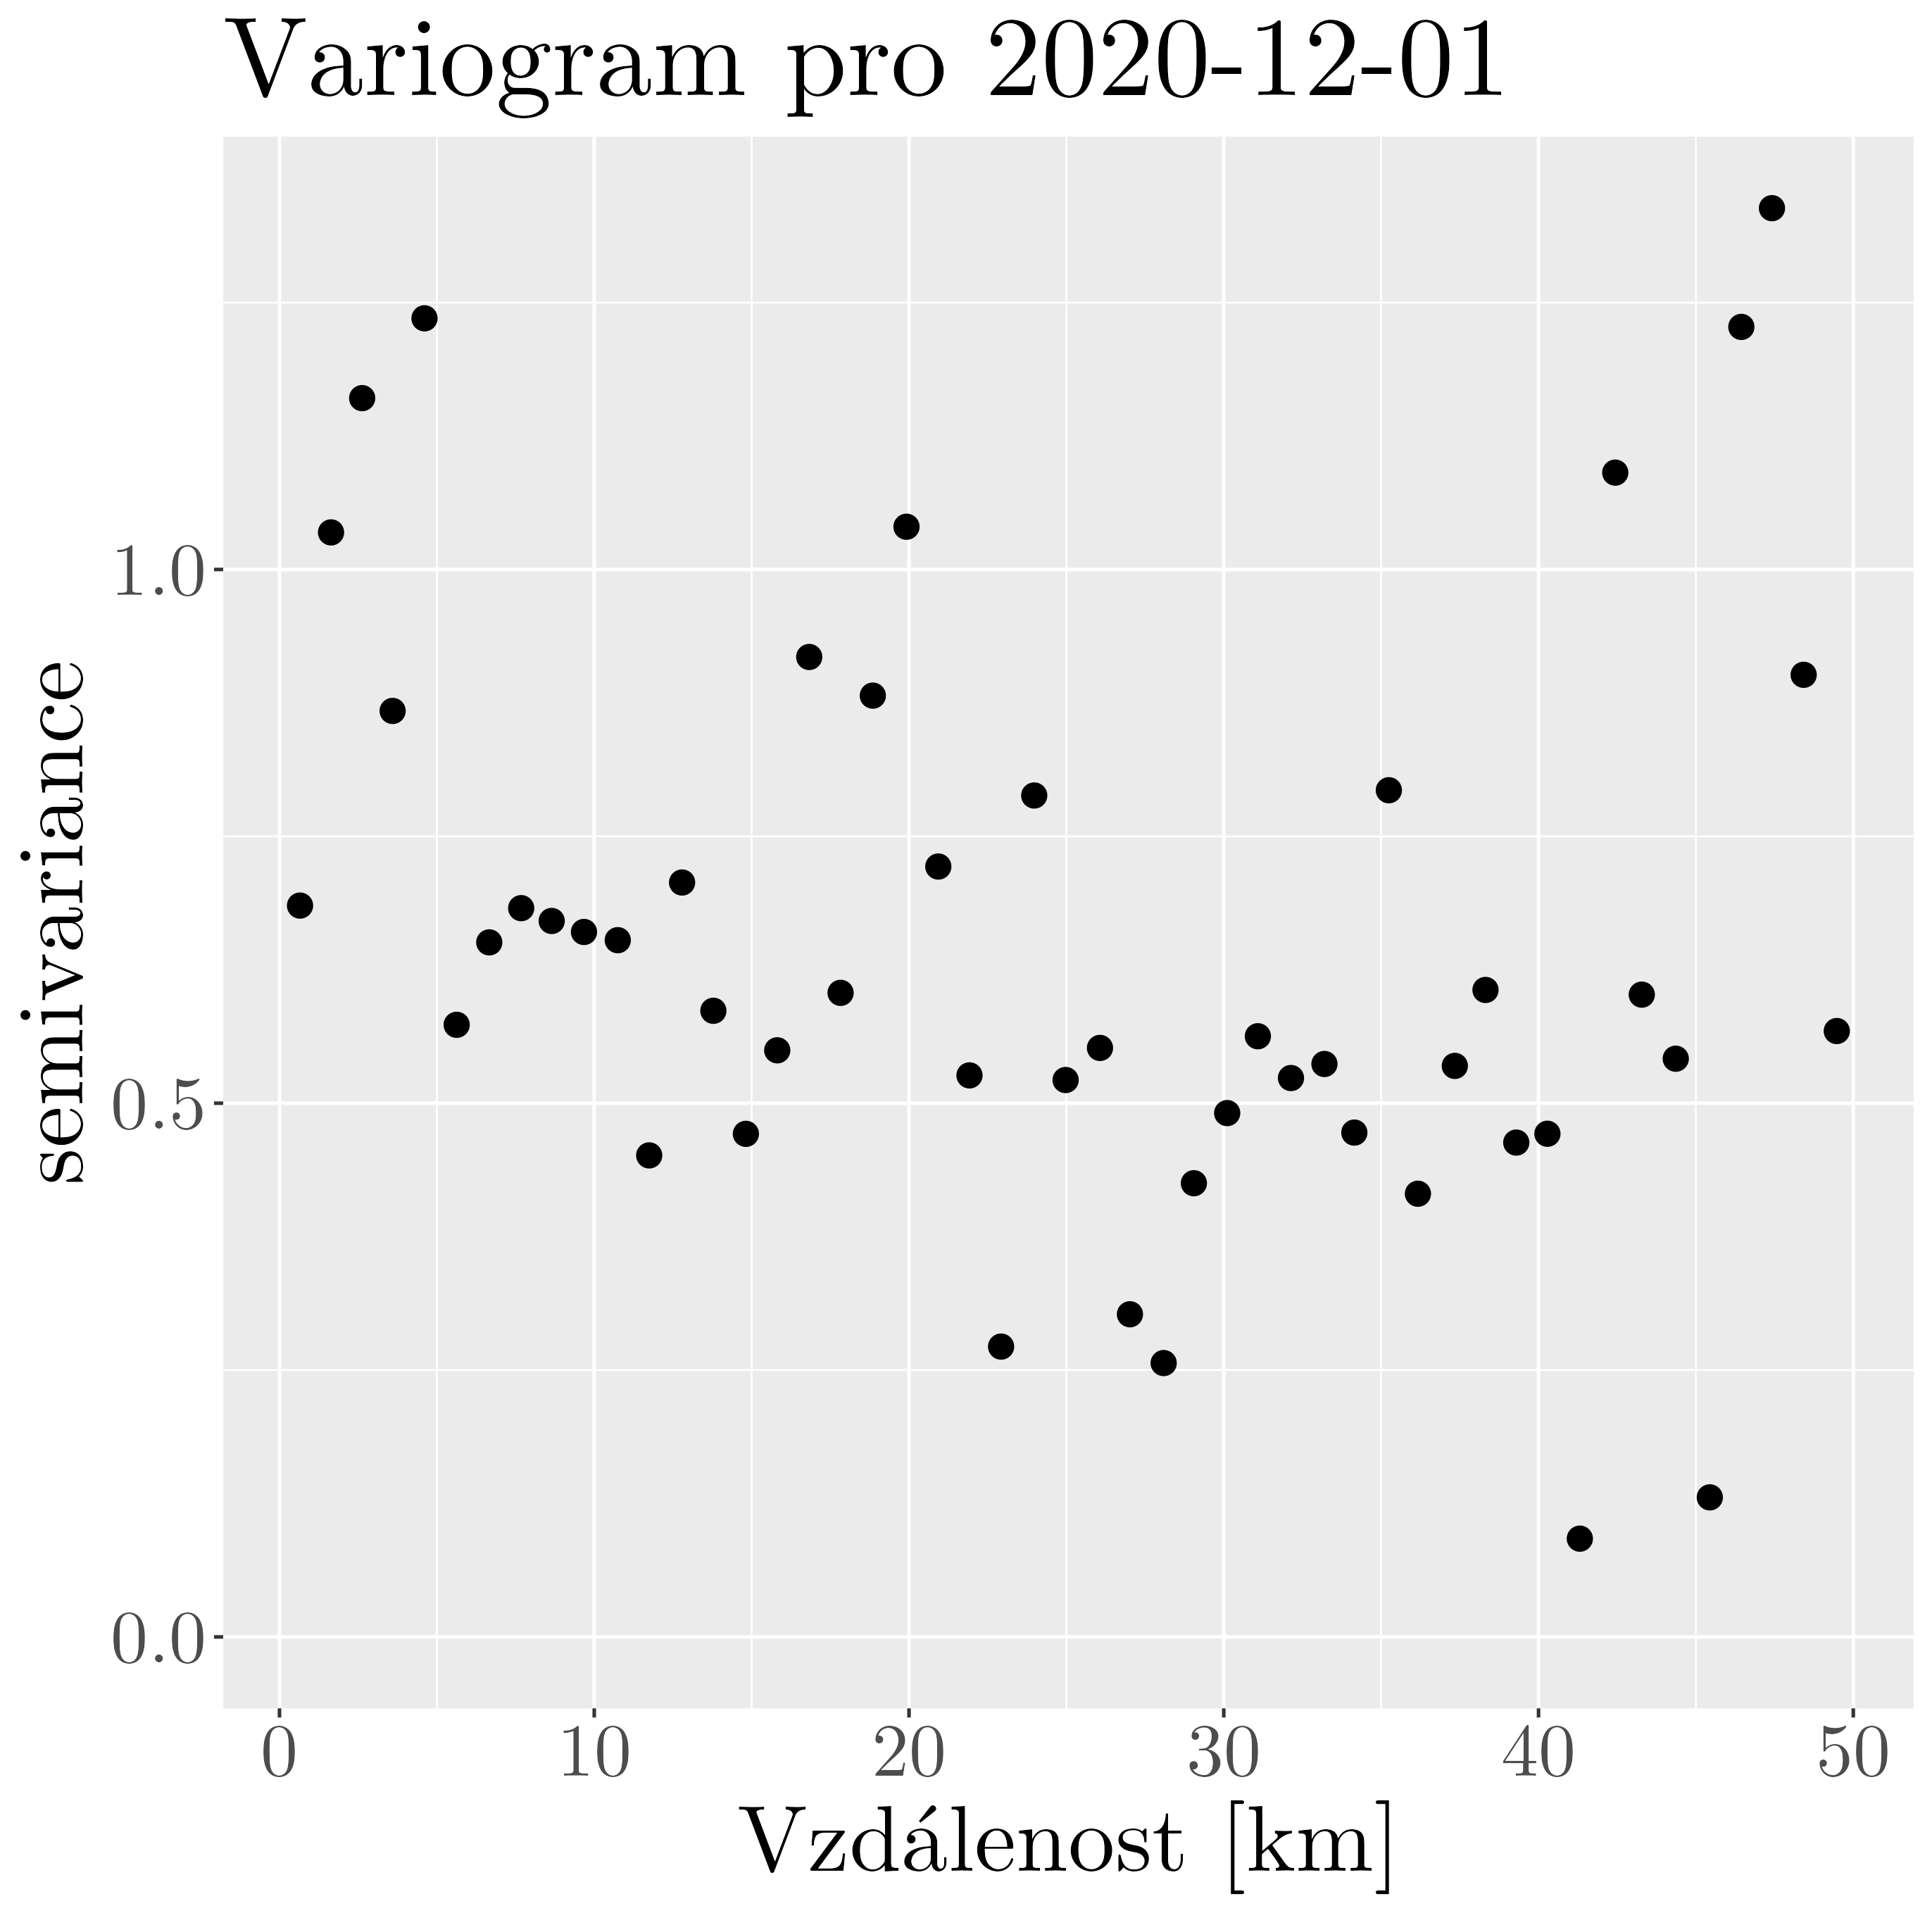
\includegraphics[width=\textwidth]{img/ch2/variograms/variogram_max15cm12.png}
		\caption{}
		\label{fig:variogram12}
	\end{subfigure}
	\caption{Semivariogramy pro jednotlivé první dny měsíců v roce 2020.}
	\label{fig:variograms}
\end{figure}

\subsection{Lineární model se smíšenými efekty}
Pro analýzu vlivu meteorologických proměnných je vhodný lineární model se smíšenými efekty popsaný v kapitole \ref{chap:lme}. Jako náhodný efekt, jehož reálná hodnota pro nás není důležitá, určíme název čidla. Pro všechna čidla a všechny dostupné dny máme kolem 78000 pozorování rozdílu maximální teploty při zemi a ve $\SI{2}{m}$ (konkrétní počet se může lišit, jestliže bereme teplotu v $\SI{0}{cm}$ nebo $\SI{15}{cm}$ nad zemí). Když vyřadíme měření, pro která chybí některá data z meteorologických stanic, a poslední čtyři dny měření, kdy máme data z menšího množství čidel, tak máme 63000 měření.

Zpracovávaná data mají šest prediktorů: insolace, srážky za poslední hodinu, celková sněhová pokrývka, oblačnost, rychlost větru a půdní vlhkost. Oblačnost nabývá diskrétních hodnot, je vyjádřena v osminách celkové oblohy, nahrazená data z ERA5 jsou vyjádřena v procentech, všechny hodnoty tedy převedeme do intervalu $0$ až $1$. Rychlost větru je měřená v diskrétních násobcích $\SI{1}{km/h}$. Ostatní prediktory, stejně jako rozdíl mezi teplotami při povrchu země, který se snažíme vysvětlit, jsou spojité proměnné. 

Pro výpočet lineárního modelu se smíšenými efekty použijeme funkci \texttt{lme} z balíčku \texttt{nlme} programovacího jazyka \texttt{R}.

Pro každý model budeme ověřovat předpoklady lineární modelu se smíšenými efekty, nyní krátce ilustrujeme problémy, s kterými se budeme v kapitole \ref{chap:ch3} potýkat, na jednom modelu. Pracujme tedy s maximální denní teplotou ve výšce $\SI{15}{cm}$ a jejím rozdílem od teploty naměřené ve $\SI{2}{m}$. Porovnáme mezi sebou transformace proměnné, kterou se snažíme vysvětlit, a to bez transformace, s logaritmem, odmocninou a třetí odmocninou. Zároveň data mají silnou autokorelaci a tudíž, použijeme pro autokorelační strukturu model ARMA s parametry $p=2$ a $q=1$ (tyto hodnoty byly vybrány vyzkoušením několika kombinací). Na obrázcích \ref{fig:qq} vidíme kvantil-kvantilový graf pro jednotlivé transformace. Hodnoty rozdílu teplot jsou ovšem i záporné, tudíž místo jednoduchého logaritmu použijeme transformaci \eqref{eq:logtrans}. Podobně ošetříme záporné hodnoty i pro ostatní transformace, jako například 3. odmocninu \eqref{eq:curttrans}. V datech se objevují i hodnoty rozdílu teplot $\Delta t=0$ pro které nemůžeme spočítat logaritmus. Jde ovšem o hodnoty pouze blízké nule, způsobené konečnou přesností čidel, tudíž na tyto hodnoty aplikujeme funkci \texttt{jitter} a tím je odlišíme od nuly a následně provedeme transformaci.

\begin{gather*}
	T \mapsto \mathrm{sign}(T)\cdot \ln\left|T\right| \label{eq:logtrans}\\
	T \mapsto \mathrm{sign}(T)\cdot \sqrt[3]{\left|T\right|} \label{eq:curttrans}
\end{gather*}

\begin{figure}
	\centering
	\begin{subfigure}{0.45\textwidth}
  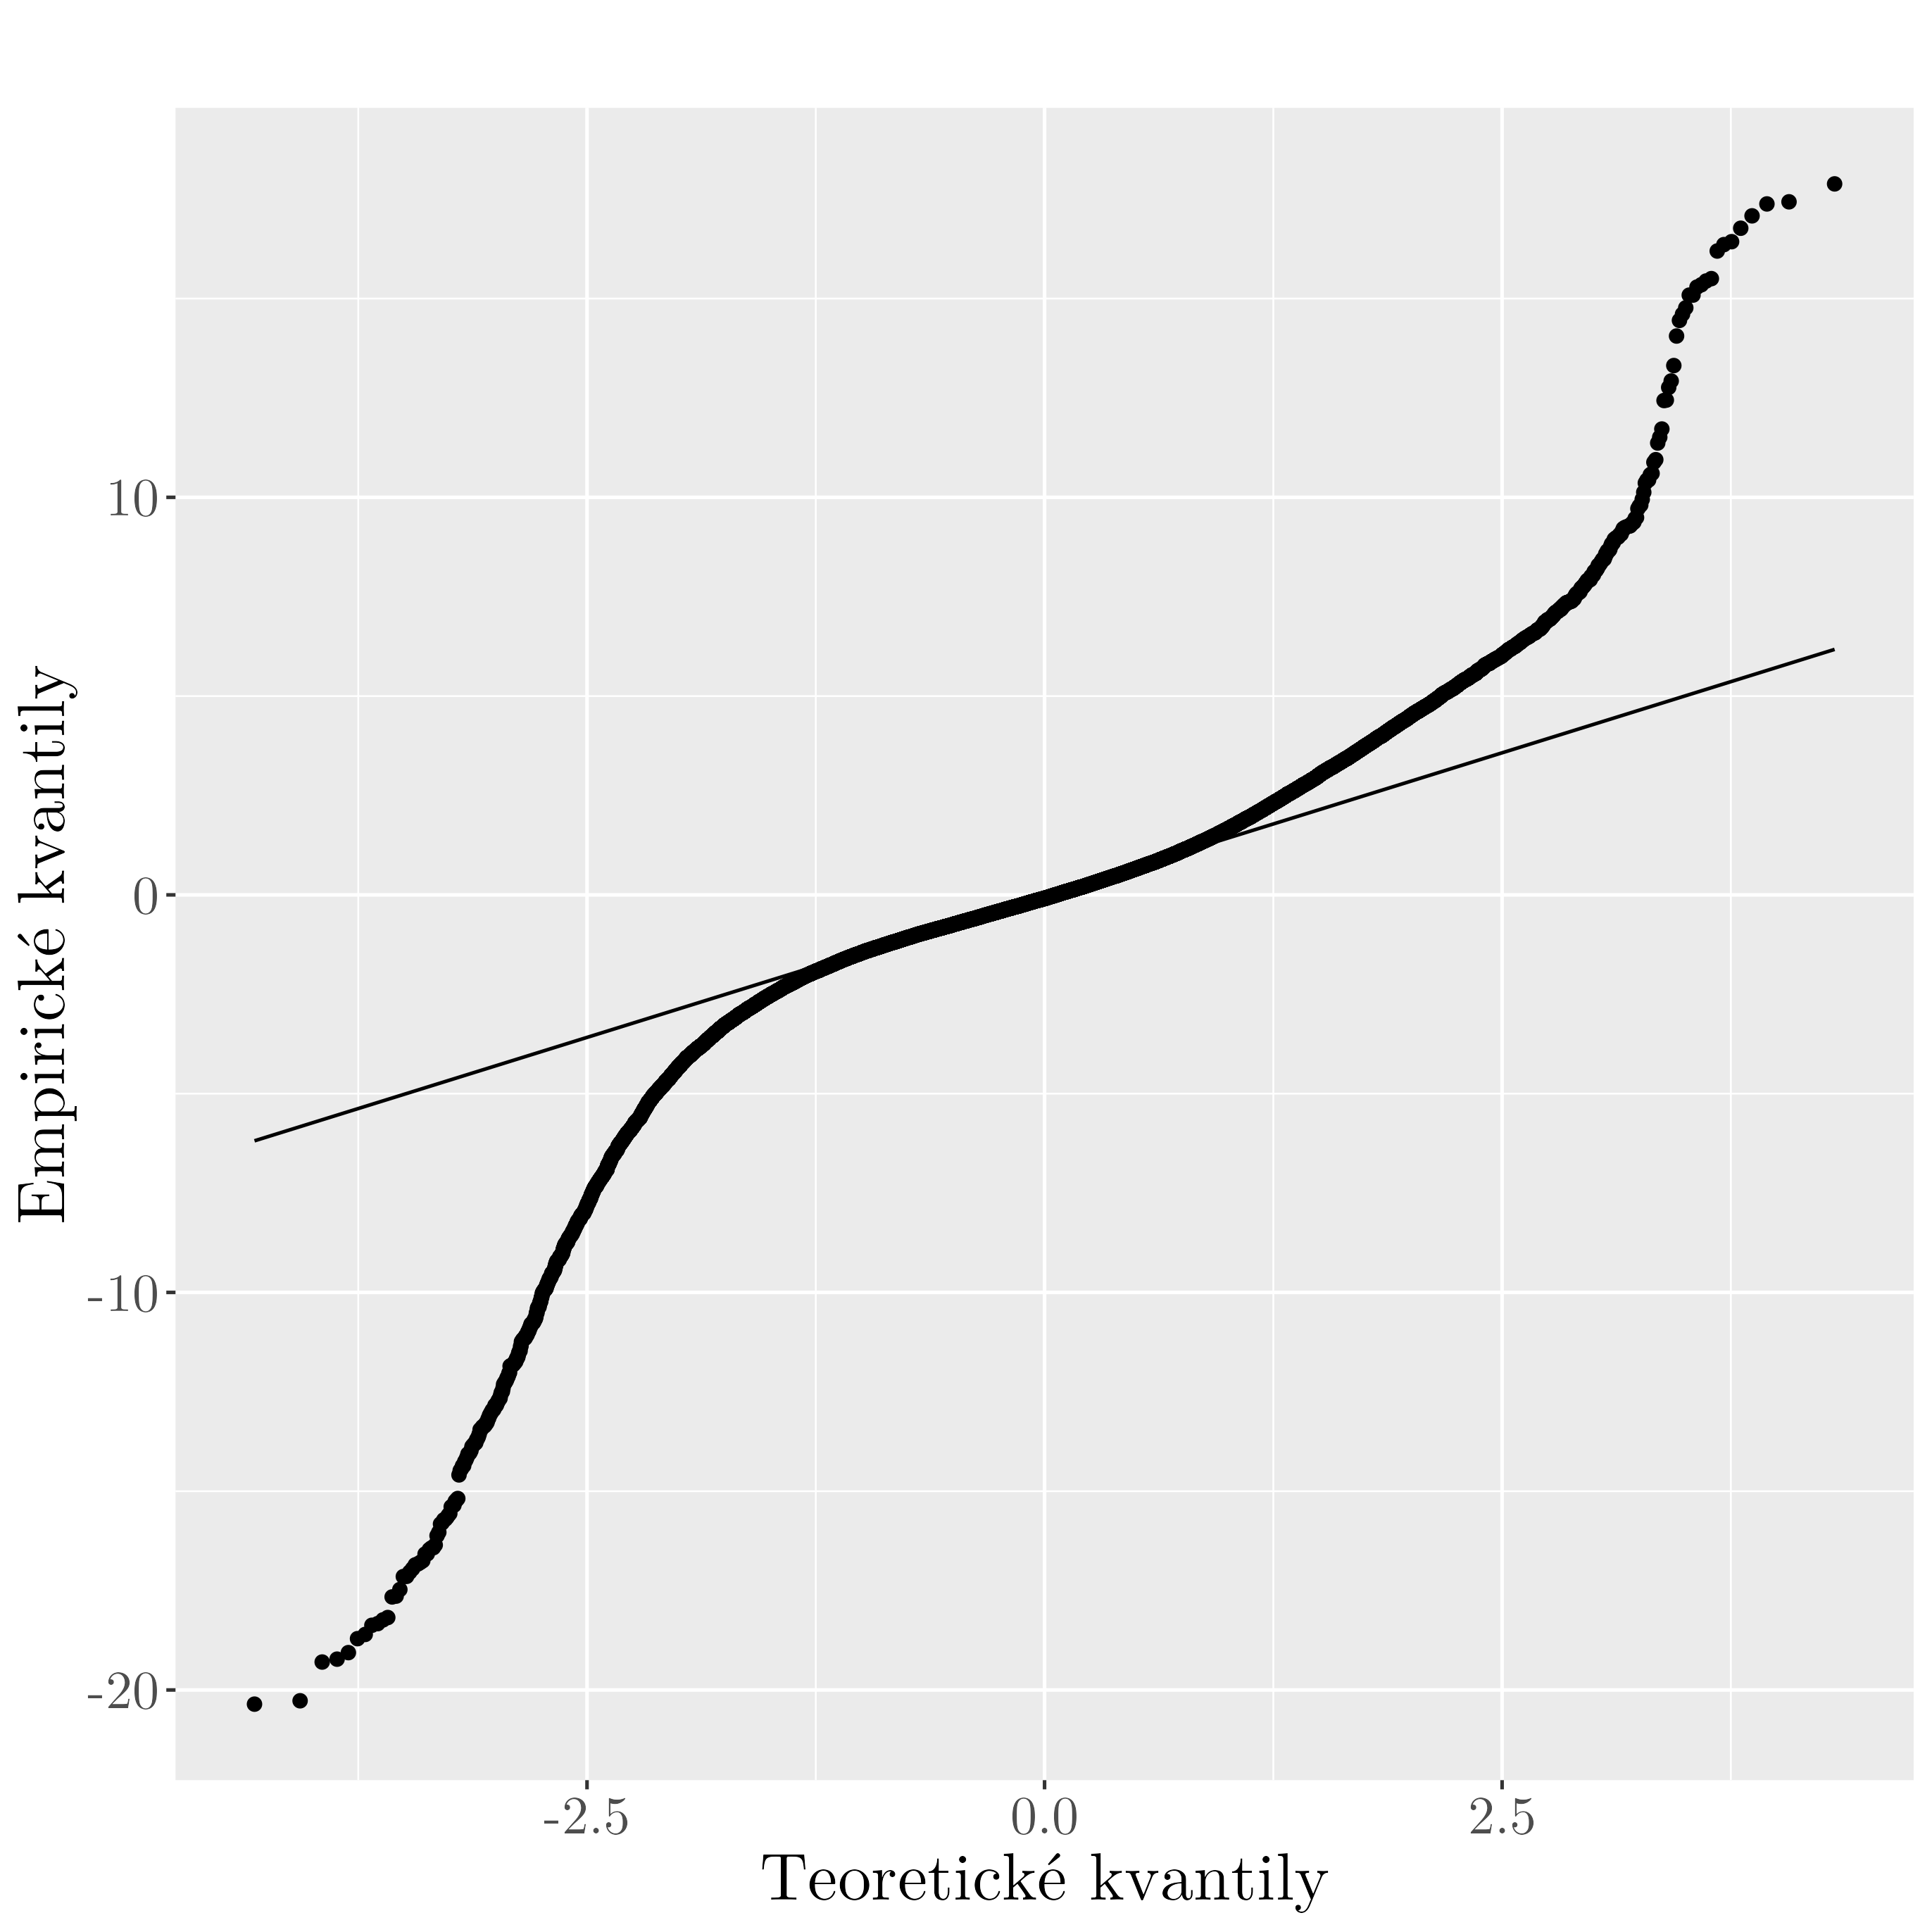
\includegraphics[width=\textwidth]{img/ch2/qq_modmax15cm_none.png}
		\caption{Bez transformace}
		\label{fig:qq_none}
	\end{subfigure}
	\hfill
	\begin{subfigure}{0.45\textwidth}
  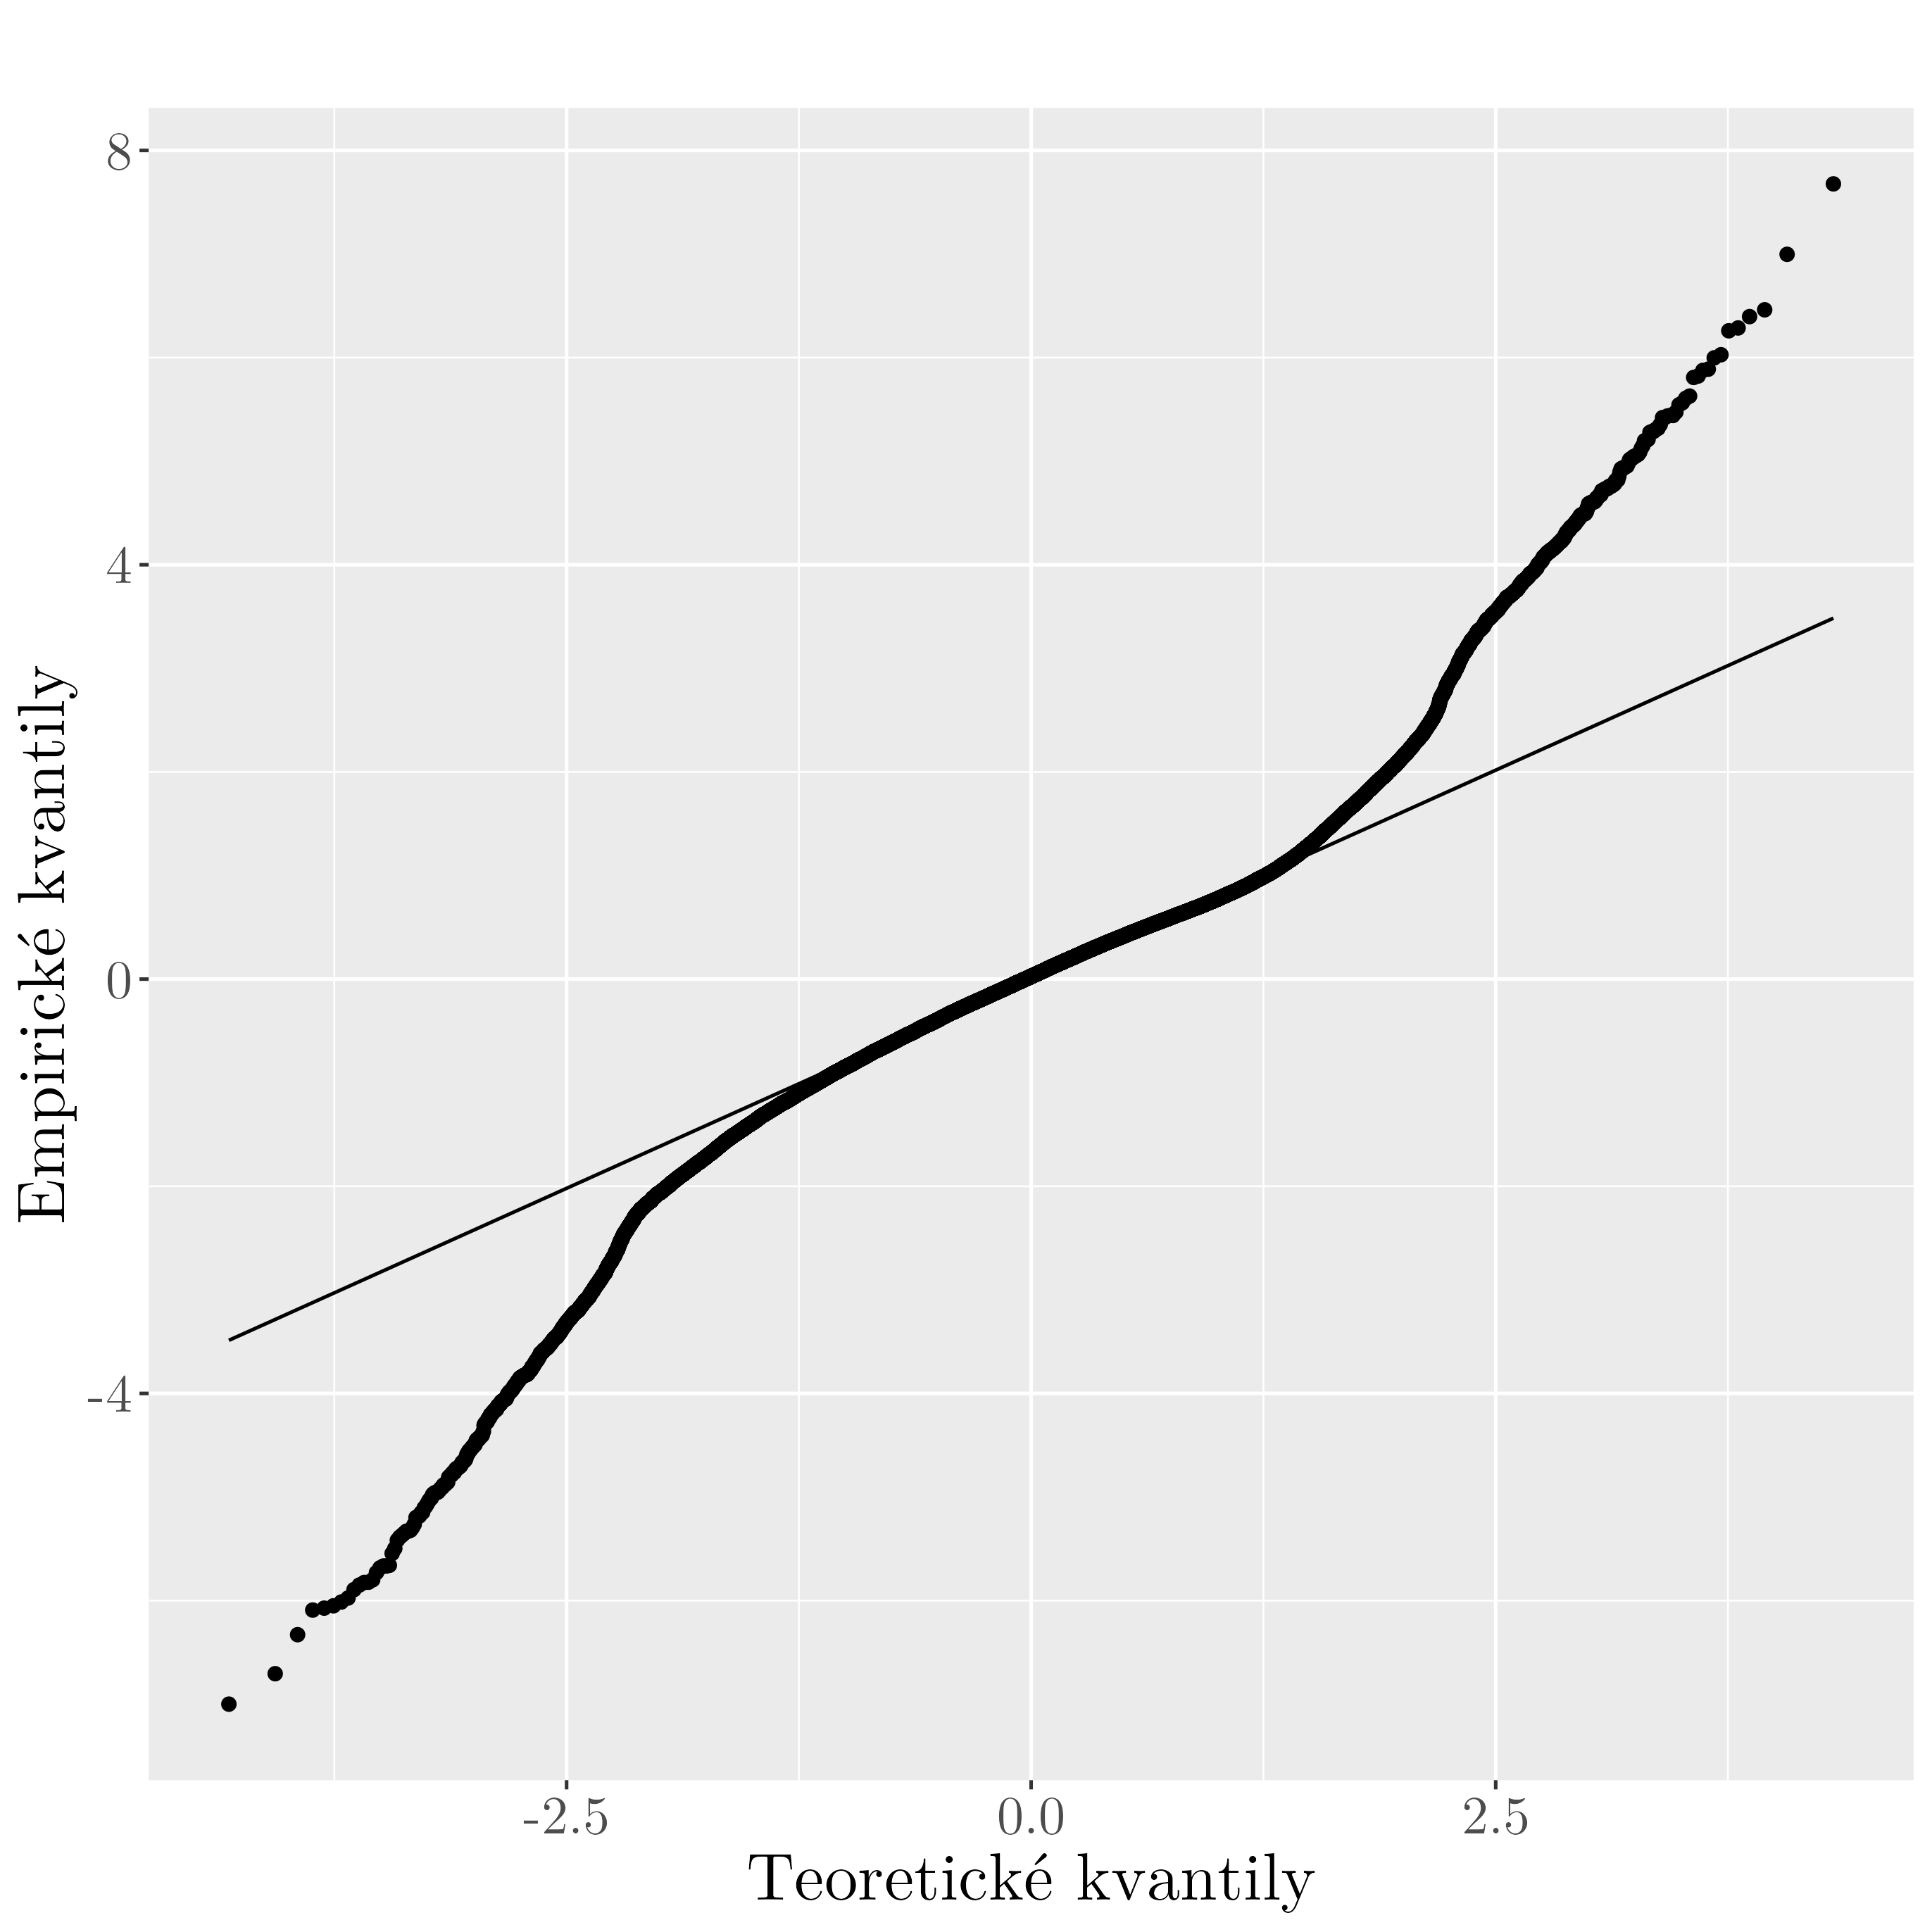
\includegraphics[width=\textwidth]{img/ch2/qq_modmax15cm_log.png}
		\caption{Přirozený logaritmus}
		\label{fig:qq_log}
	\end{subfigure}
	\hfill
	\begin{subfigure}{0.45\textwidth}
  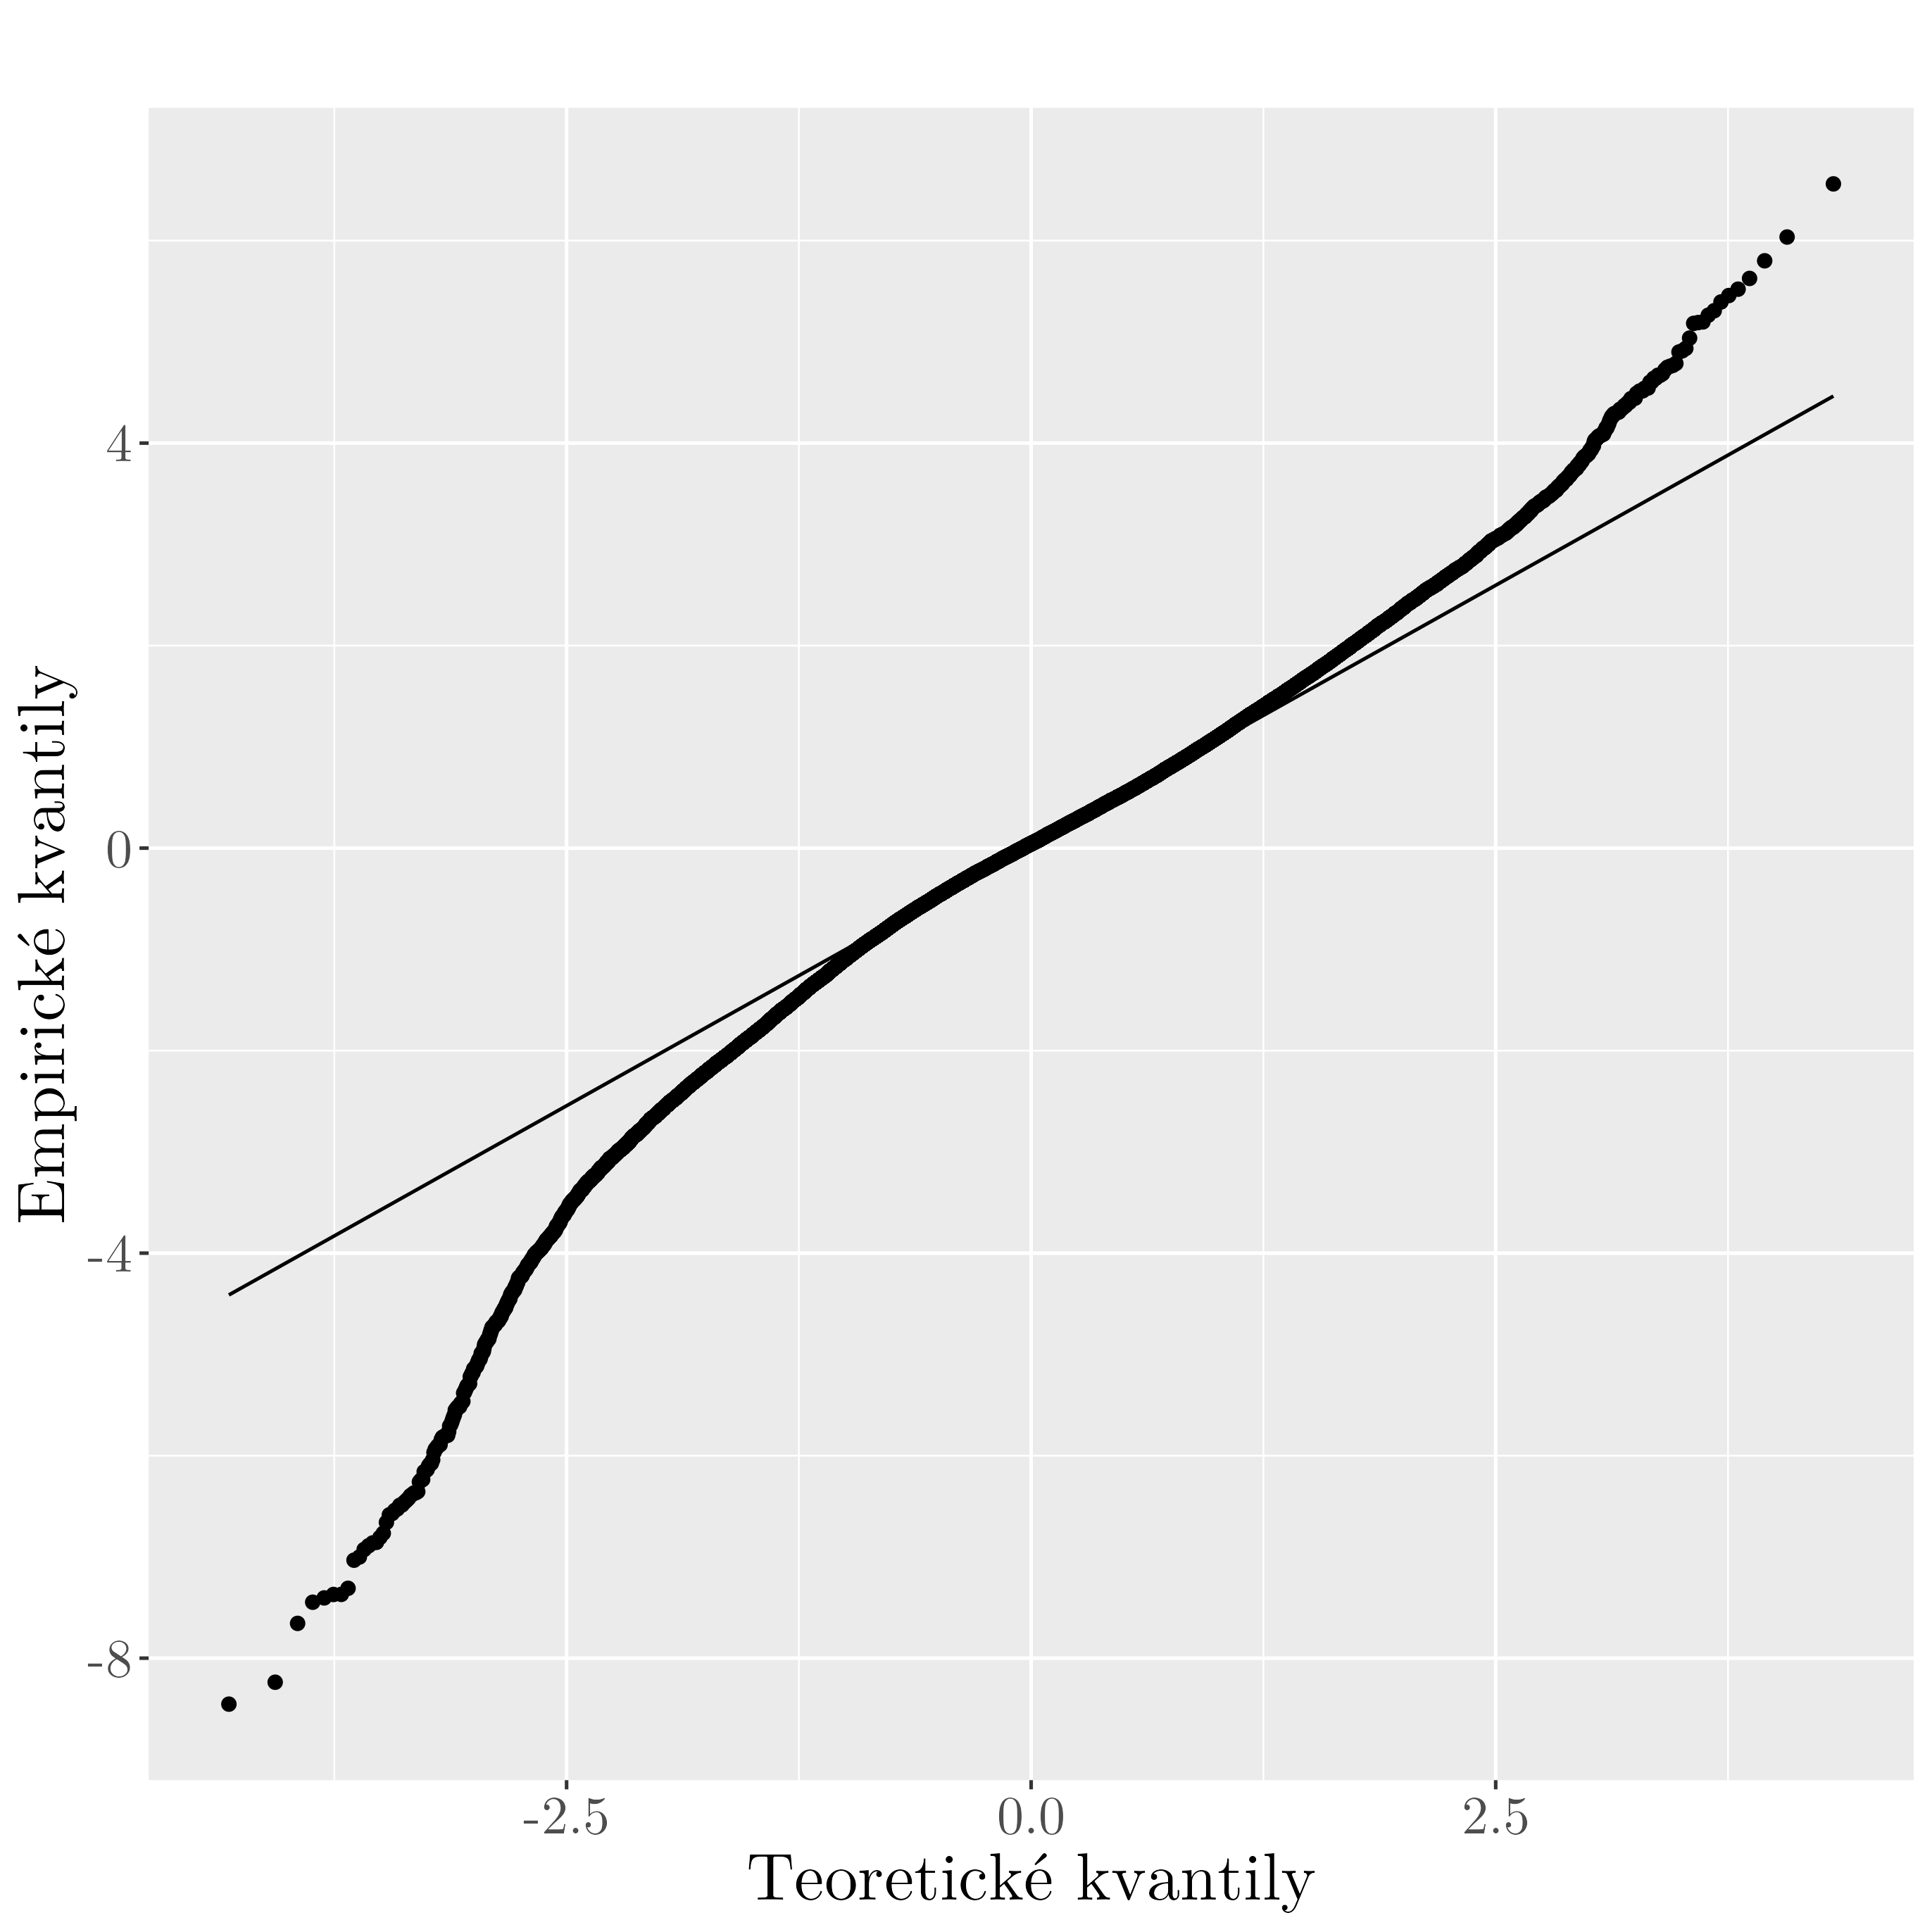
\includegraphics[width=\textwidth]{img/ch2/qq_modmax15cm_sqrt.png}
		\caption{Druhá odmocnina}
		\label{fig:qq_sqrt}
	\end{subfigure}
	\hfill
	\begin{subfigure}{0.45\textwidth}
  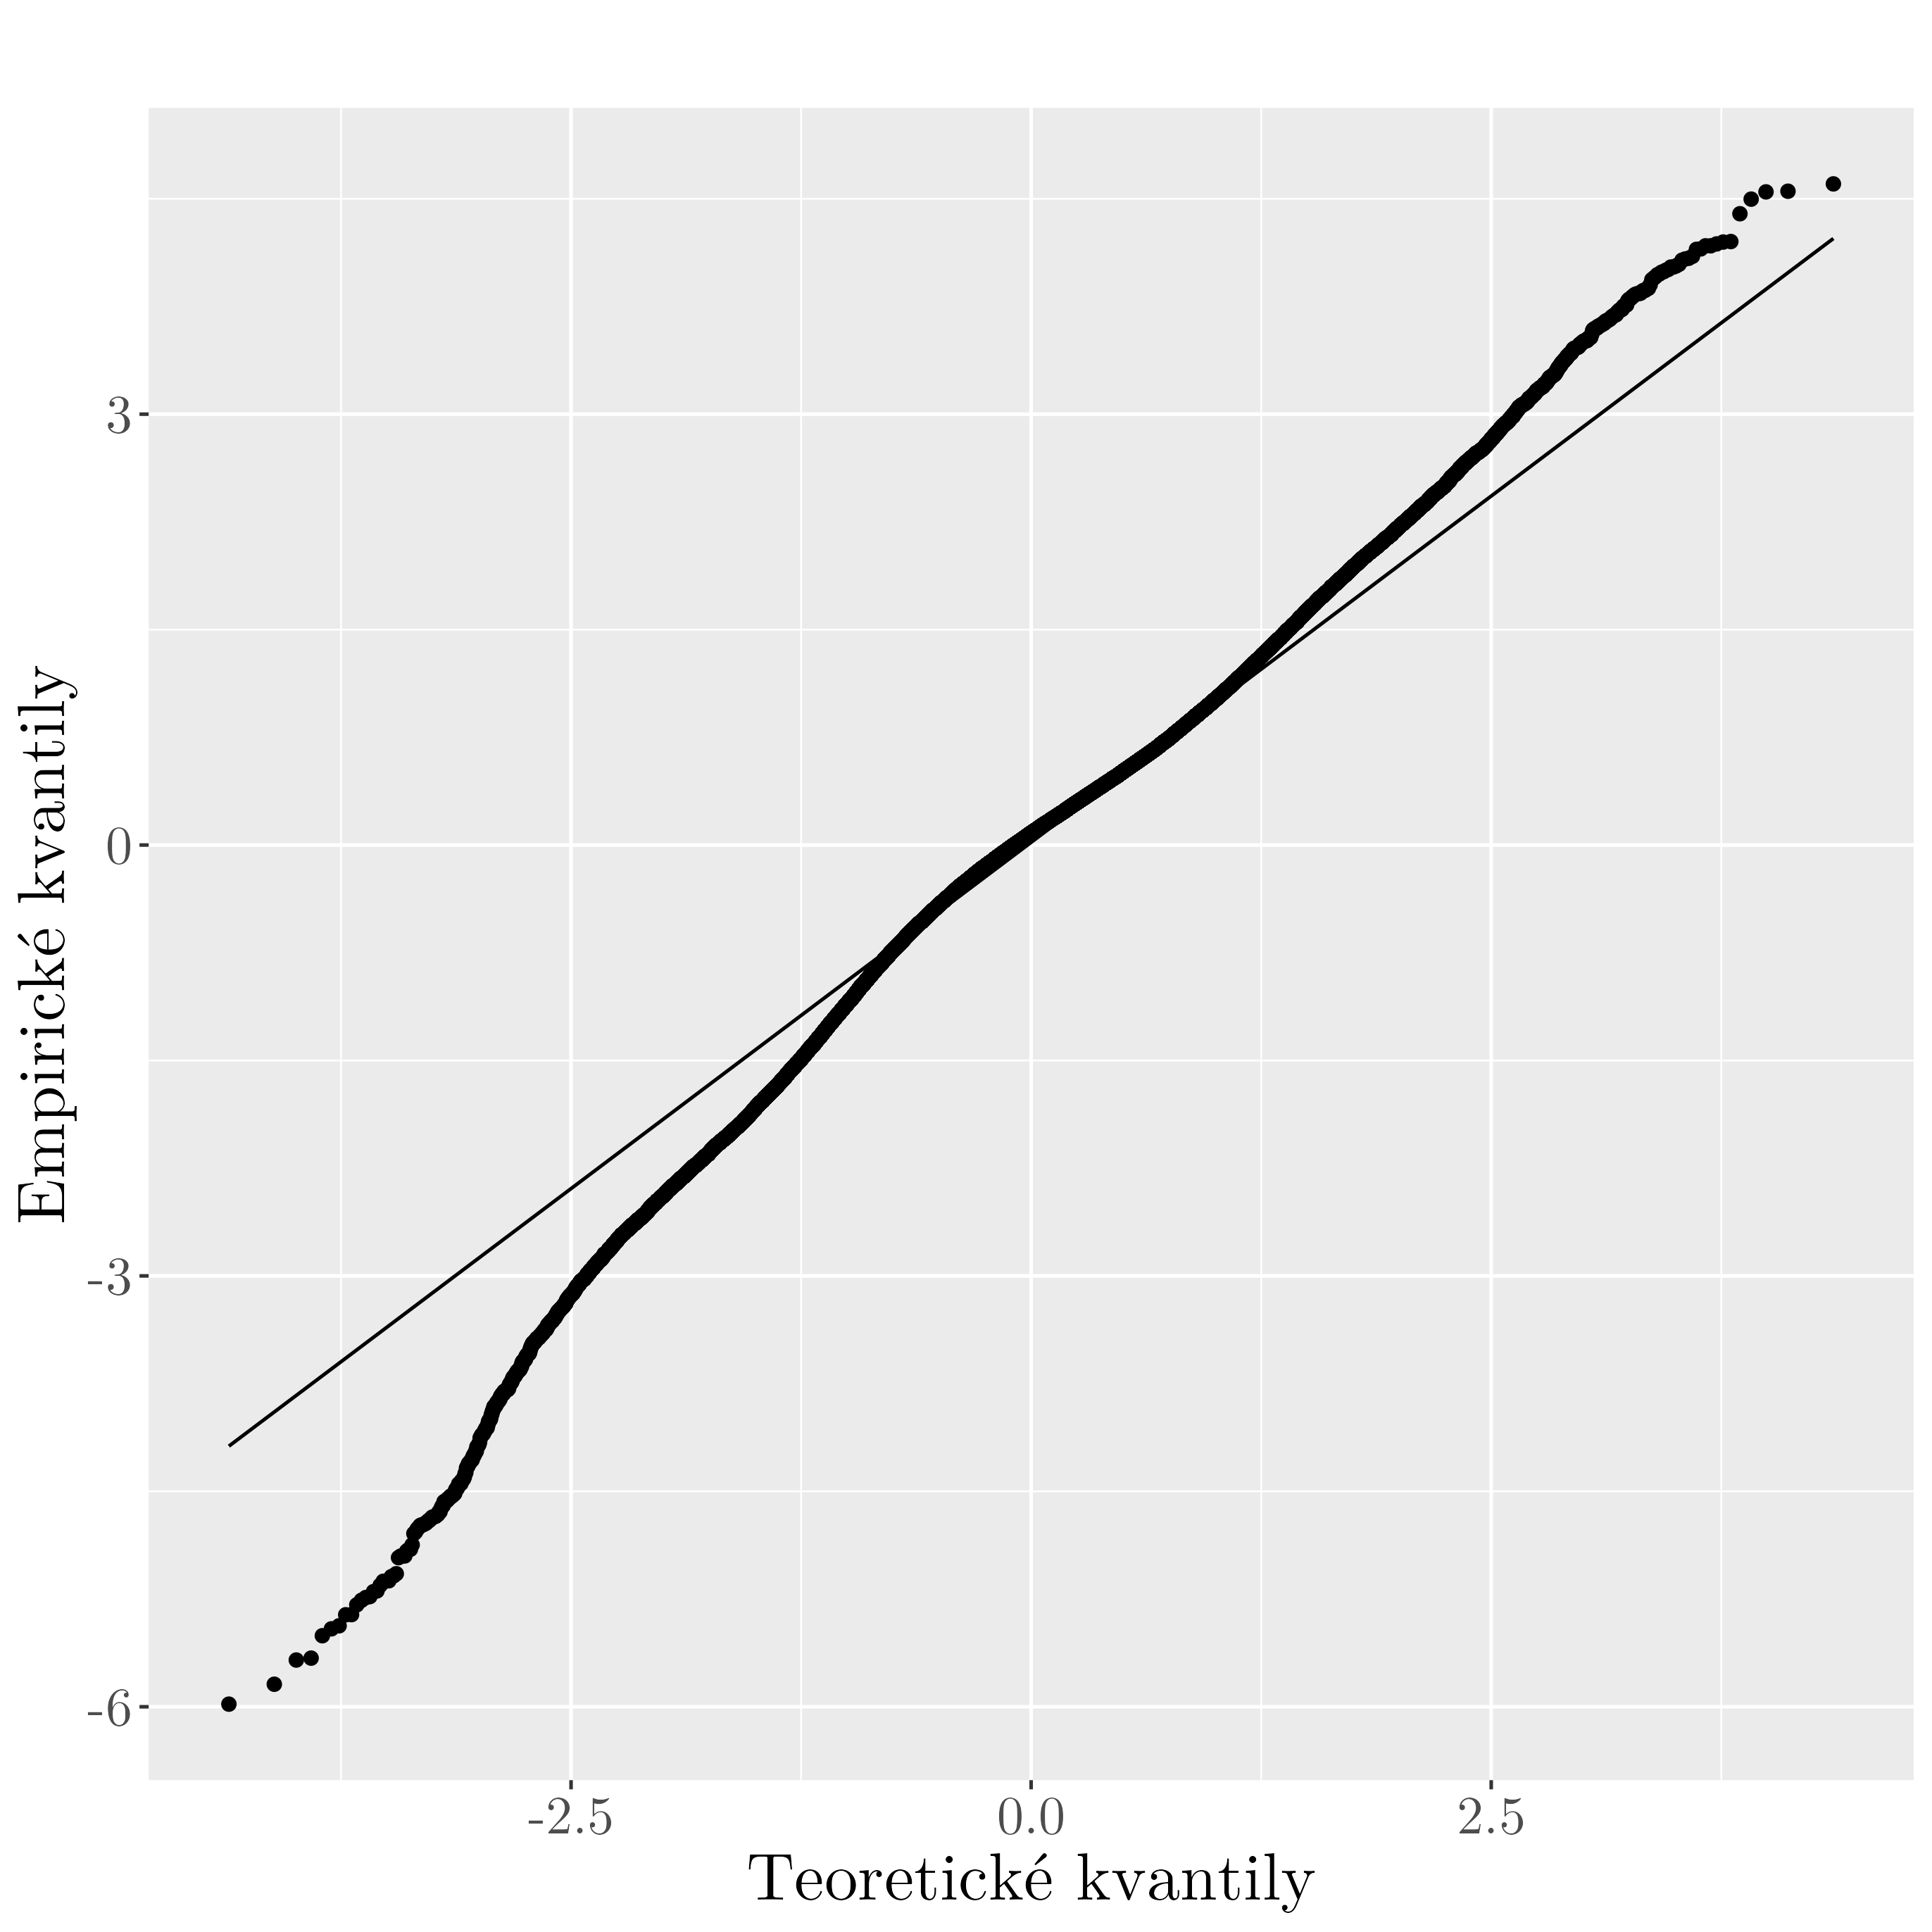
\includegraphics[width=\textwidth]{img/ch2/qq_modmax15cm_curt.png}
		\caption{Třetí odmocnina}
		\label{fig:qq_curt}
	\end{subfigure}
	\caption{Kvantil-kvantilový graf pro jednotlivé transformace vysvětlované proměnné.}
	\label{fig:qq}
\end{figure}

Vidíme, že nejlépe normálnímu rozdělení odpovídá transformace třetí odmocniny a proto s ní budeme nadále pracovat. Transformace ovšem není dokonalá, stále jsme se úplně nezbavili šikmosti (skewness). Formální testy normálity rozdělení jako například Shapiro-Wilkův test se zde nehodí, neboť jsou velmi náchylné na malé odchylky od normálního rozdělení \parencite{shapirowilk}. Na obrázku \ref{fig:resvsfit_curt} můžeme vidět srovnání residuálů modelu s fitovanými hodnotami. Na obrázku můžeme vidět, že v takto transformovaných datech není výrazná heteroskedasticita.

Homoskedasticitu budeme ověřovat graficky, pomocí srovnání fitovaných hodnot a residuálů modelu. Pokud nebyl porušen předpoklad homoskedasticity, tak nesmíme pozorovat závislost mezi fitovanými hodnotami a residuály, jak bylo popsáno v kapitole \ref{chap:lme}. Na obrázku \ref{fig:resvsfit_curt} vidíme srovnání residuálů modelu s fitovanými hodnotami a není zde žádná výrazná heteroskedasticita.

\begin{figure}
	\centering
  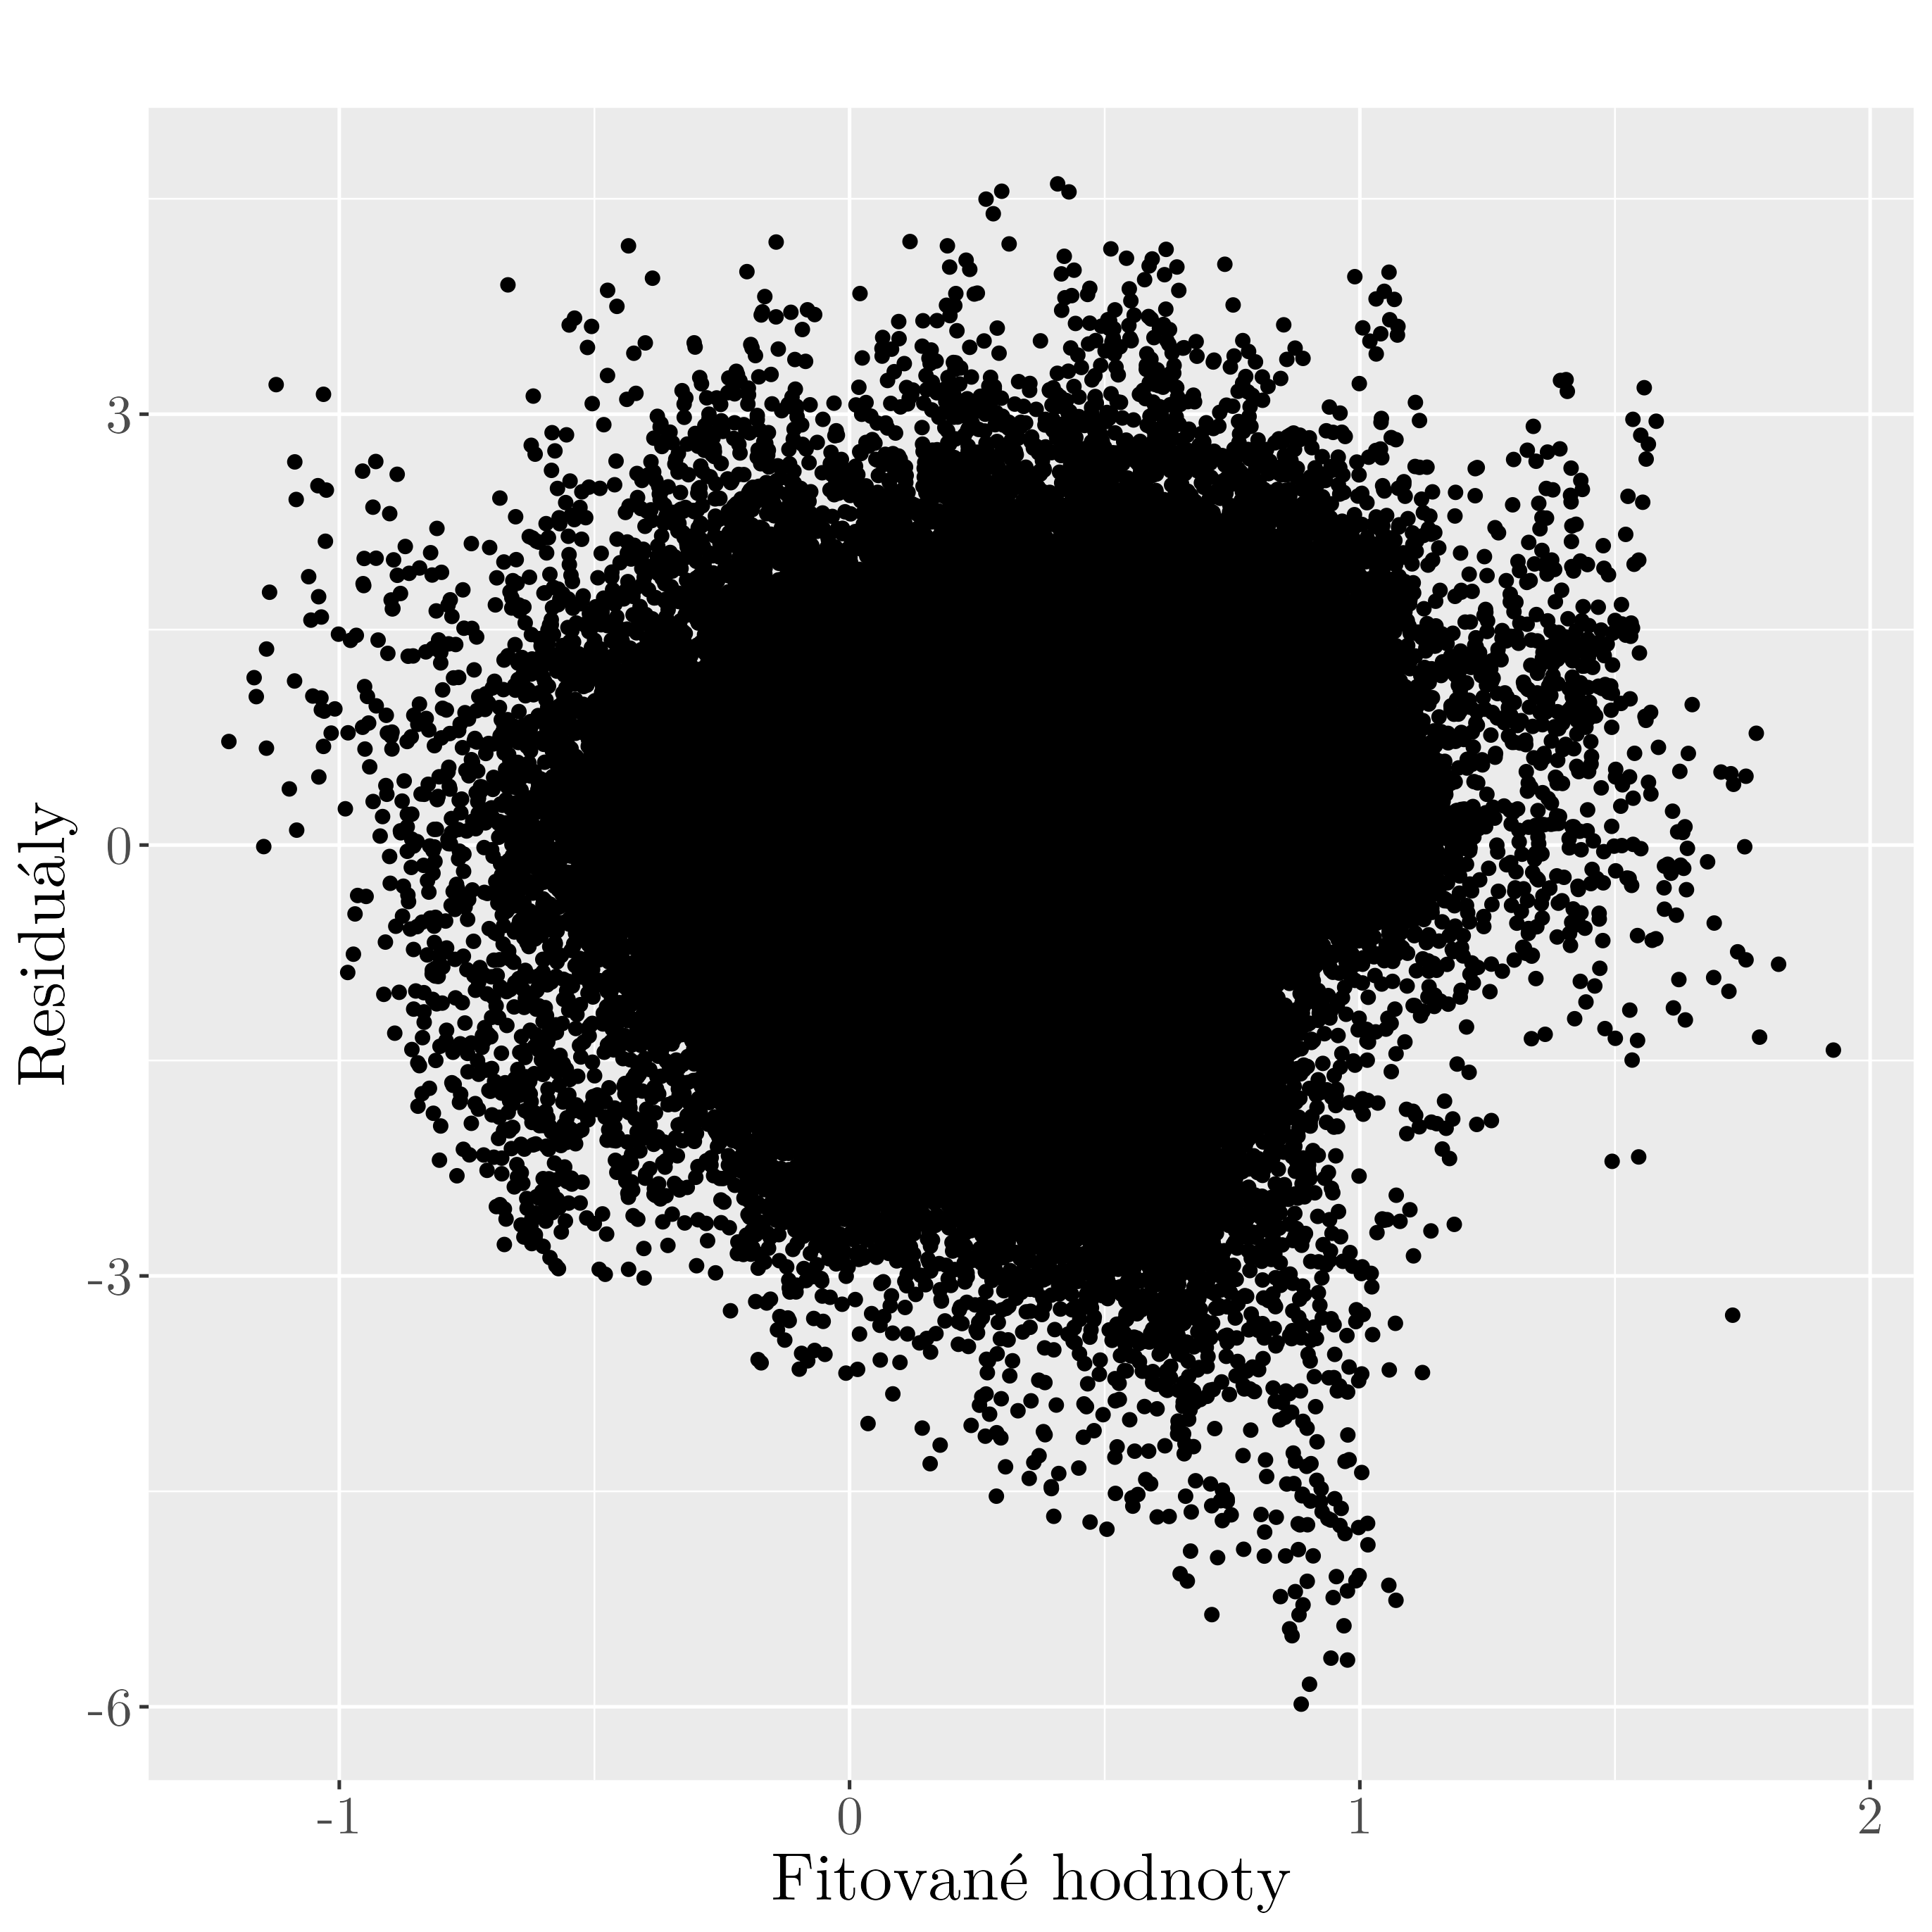
\includegraphics[width=0.55\textwidth]{img/ch2/modmax15cm_curt.png}
	\caption{Srovnání residuálů modelu s fitovanými hodnotami pro transformaci pomocí třetí odmocniny.}
	\label{fig:resvsfit_curt}
\end{figure}

Pro ilustraci důležitosti ARMA modelu na obrázku \ref{fig:acf_curtnoARMA} autokorelační funkci bez modelu ARMA a na \ref{fig:acf_curtARMA22} s modelem ARMA. Hodnota $\text{ACF}$ pro $\text{lag}=0$ je vyřazená pro větší přehlednost grafu, vždy nabývá hodnoty $1$.

Vidíme, že přidání ARMA s hodnotami ($p=2$ a $q=1$) se výrazně zlepší autokorelační funkce a korelační strukturu jsme téměř odfiltrovali. Testovali jsme i jiné hodnoty $p$ a $q$, ale pro $p=2$ a $q=1$ nám vyšla autokorelační funkce nejlepší. S rostoucím $p$ a $q$ také roste výpočetní náročnost, pro $p=3$ a $q=3$ se ACF téměř nezmění, ale výpočet trvá až 4-krát déle (na počítači, který byl používán ke zpracování, šlo o více než 3 hodiny výpočetního času).

\begin{figure}
	\centering
	\begin{subfigure}{0.45\textwidth}
  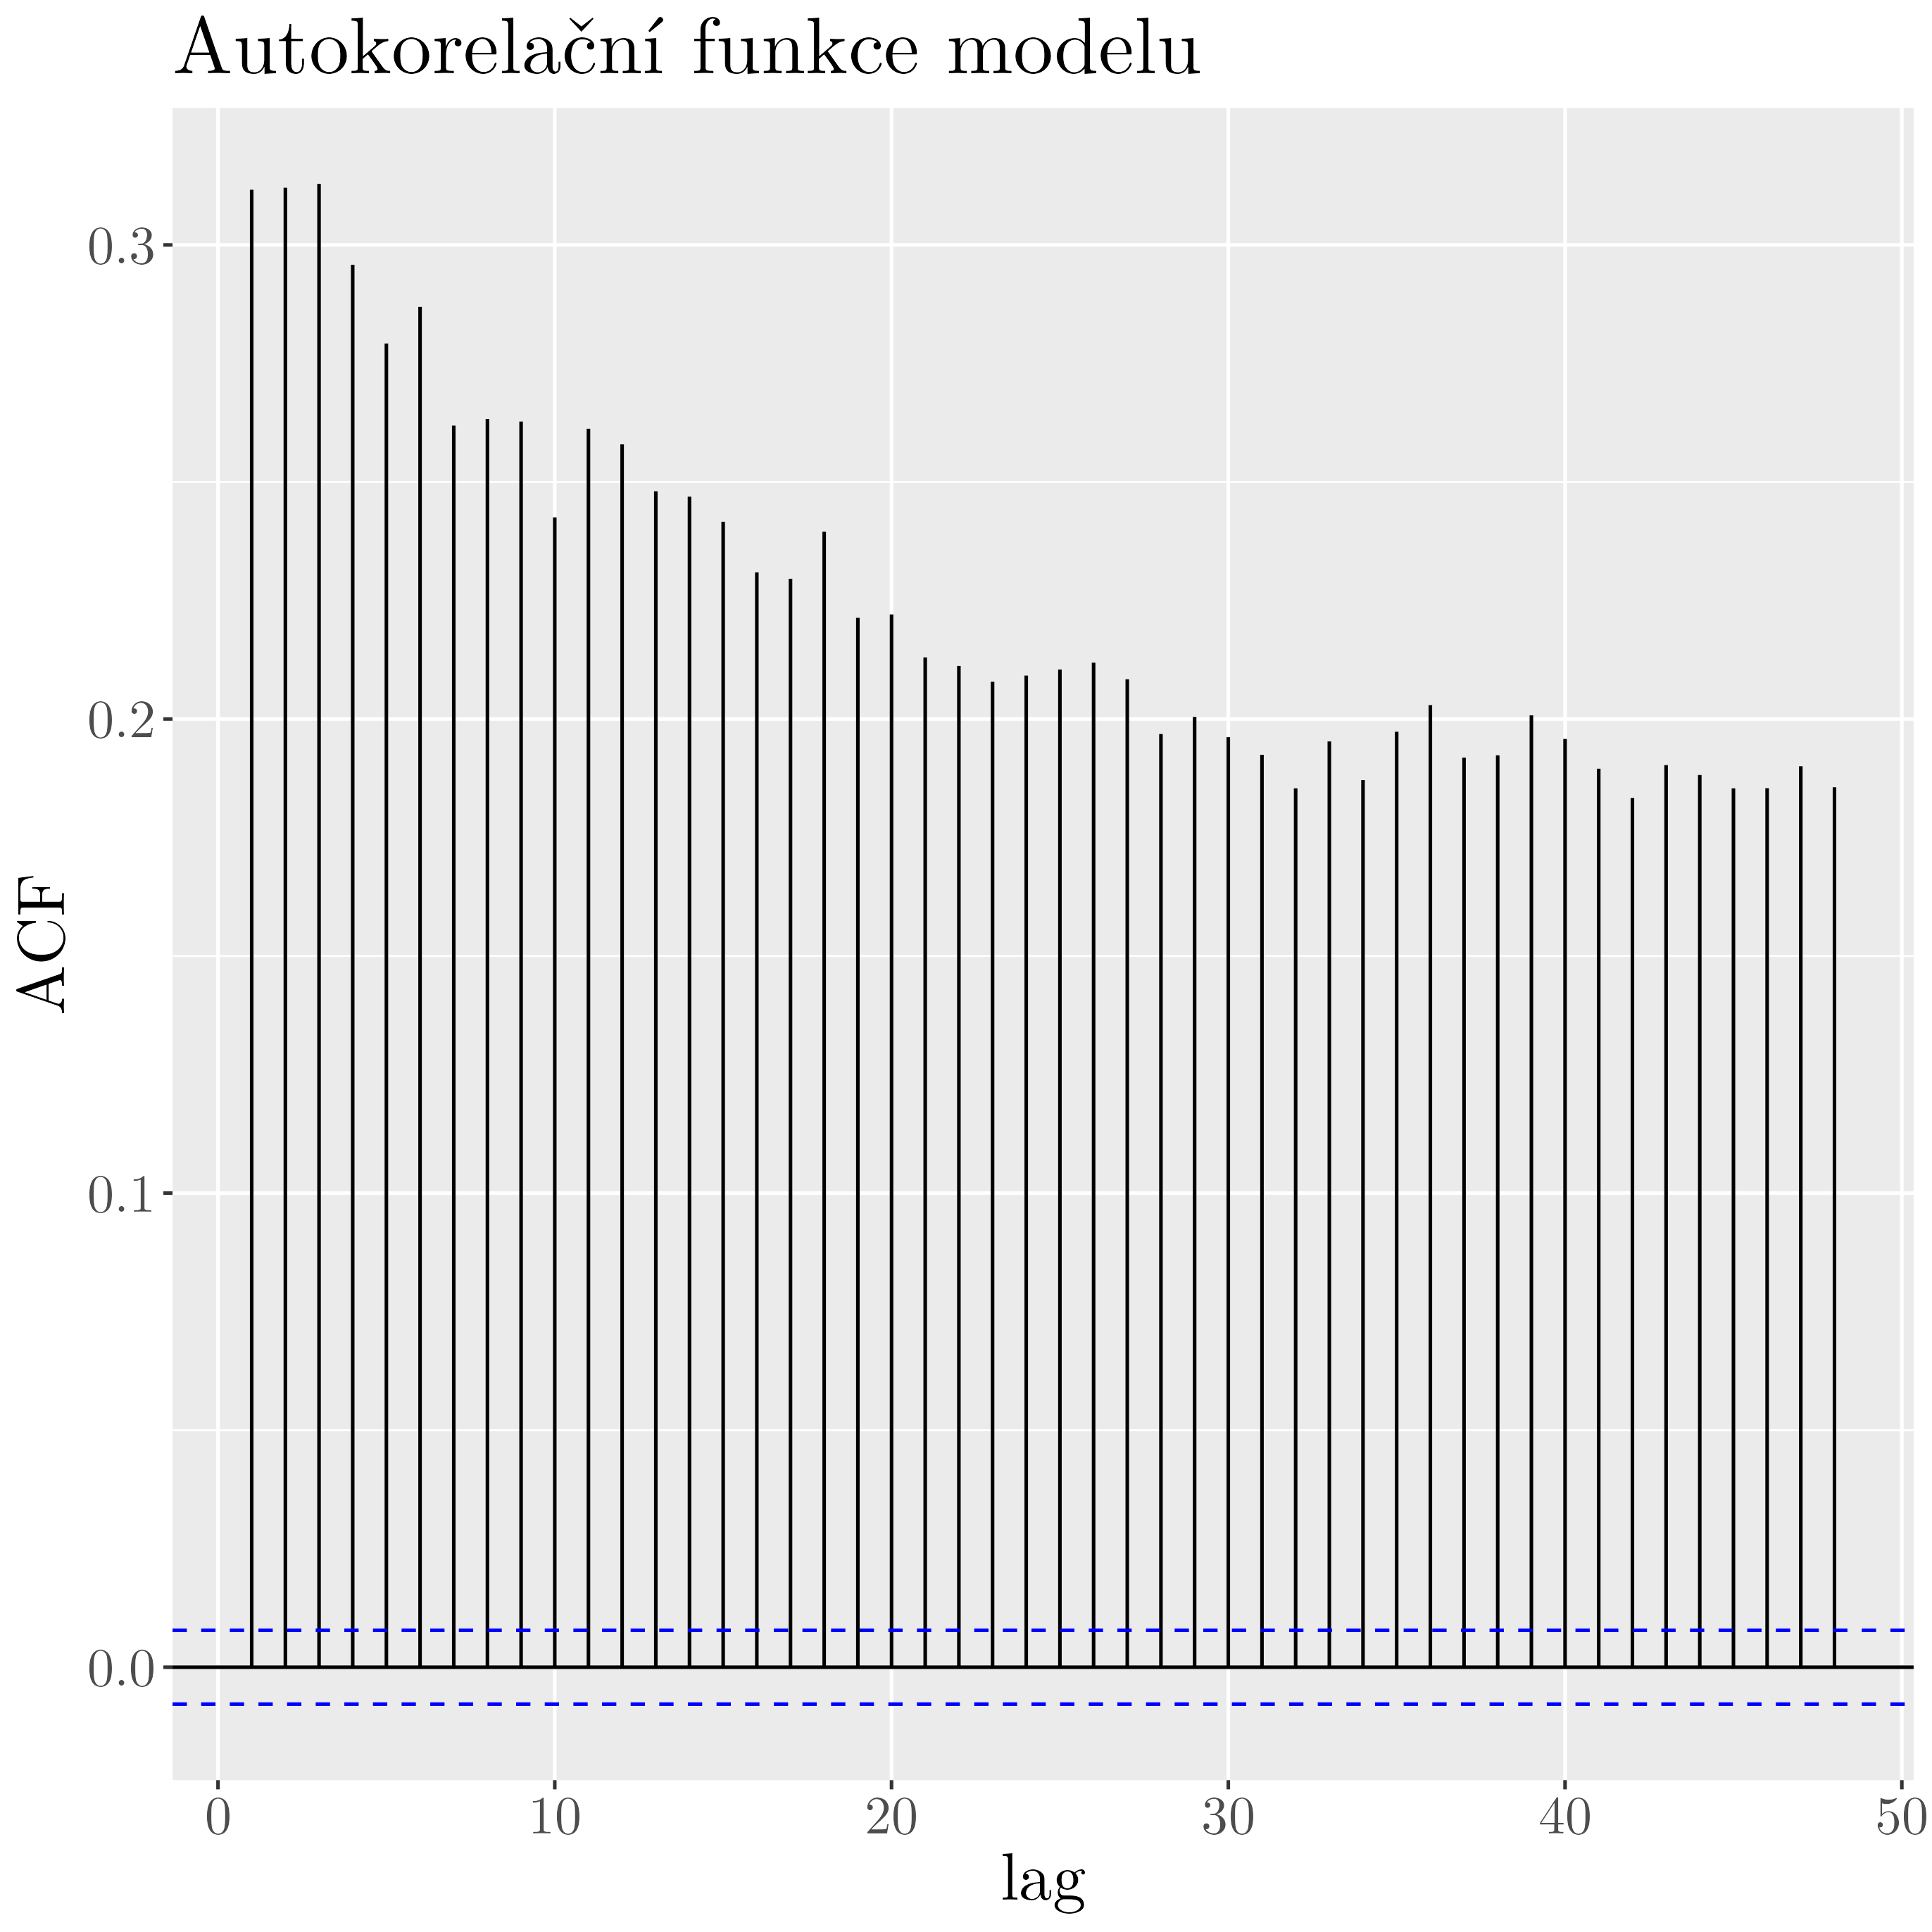
\includegraphics[width=\textwidth]{img/ch2/acf_curt.png}
		\caption{Autokorelační funkce pro model s transformací $\sqrt[3]{}$, ale bez modelování autokorelační struktury.}
		\label{fig:acf_curtnoARMA}
	\end{subfigure}
	\hfill
	\begin{subfigure}{0.45\textwidth}
  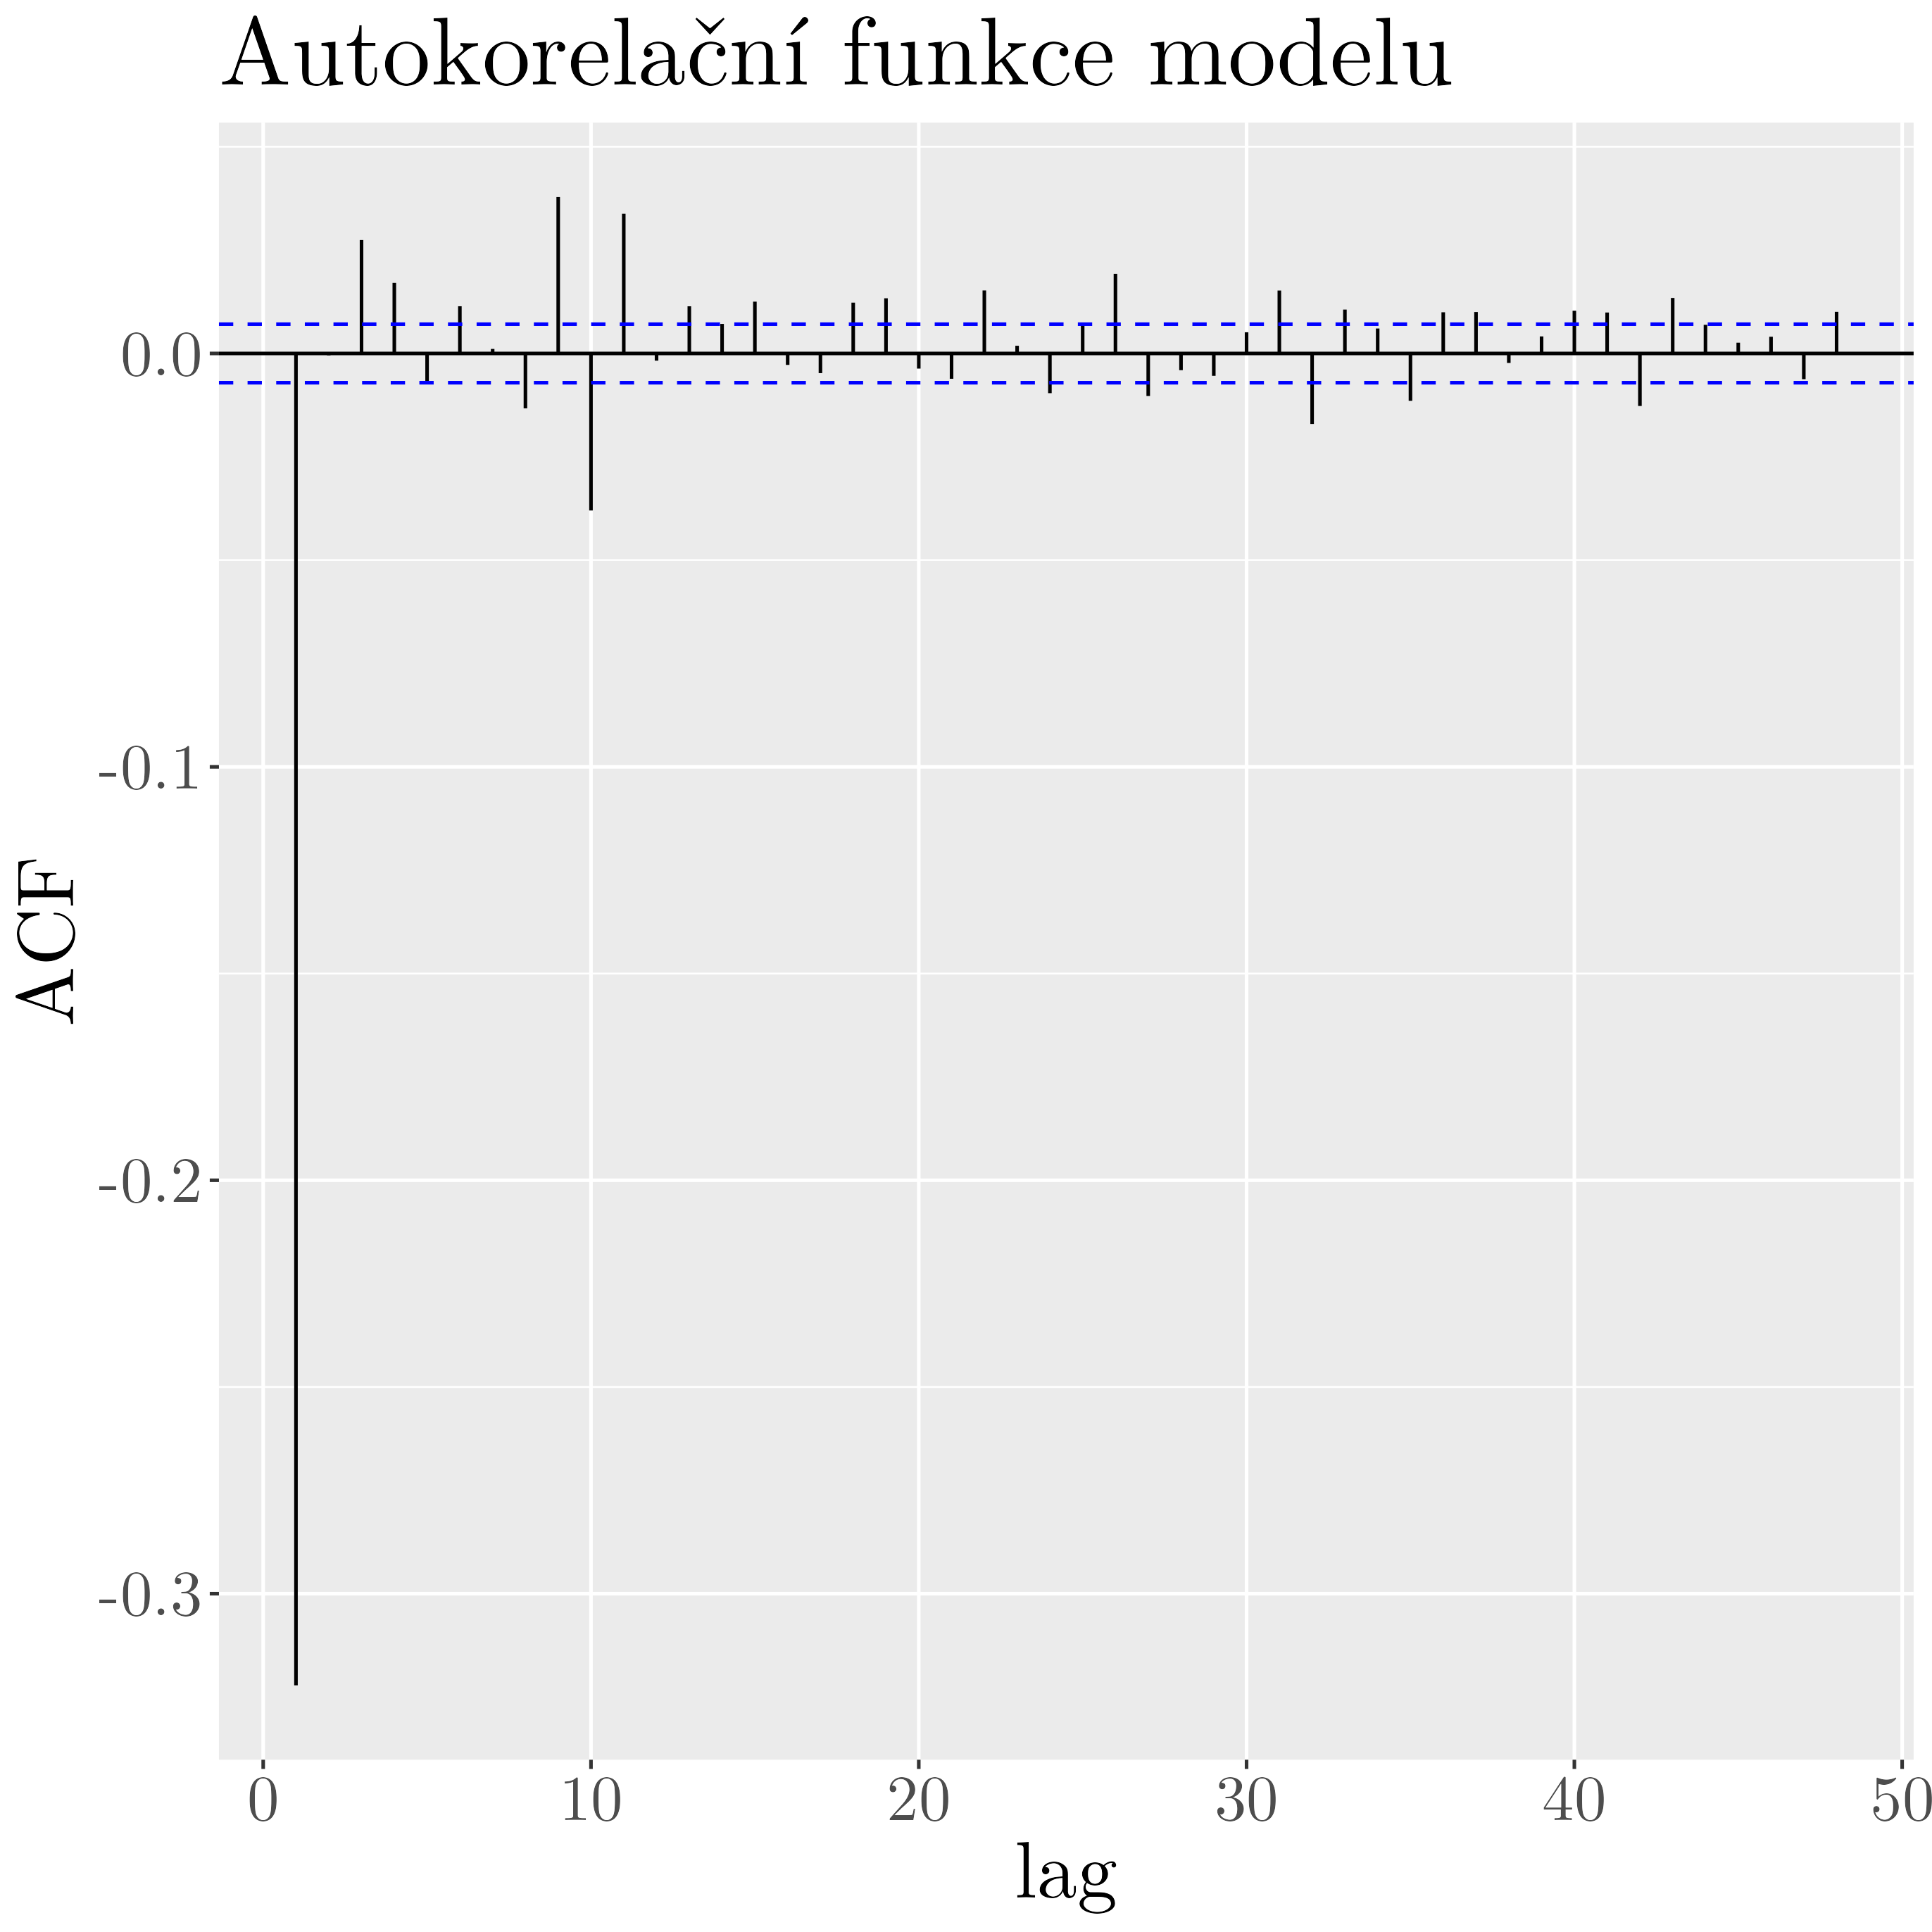
\includegraphics[width=\textwidth]{img/ch2/acf_curtARMA22.png}
		\caption{Autokorelační funkce pro model s transformací $\sqrt[3]{}$, s modelování autokorelační struktury, kde $p=2,\ q=1$.}
		\label{fig:acf_curtARMA22}
	\end{subfigure}
	\caption{Srovnání autokorelační funkce modelu s a bez ARMA}
	\label{fig:acf_curt}
\end{figure}

\subsection{Seznam modelů}
Výše jsme ukázali, jakým způsobem zpracováváme jednotlivé modely. Pro přehlednost označujeme modely zkratkou, abychom nemuseli vždy vypisovat pro které období byl model počítán nebo jestli jde o maximálně nebo minimální denní teploty. Seznam modelů je v tabulce \ref{tab:seznammodelu}. K těmto 16 modelům jsme přidali ještě dalších 16 modelů, které mají stejné parametry, ale místo rozdílu teplot např. $\Delta t = t_{15cm} - t_{2m}$ jako závislou proměnnou bereme její absolutní hodnotu, jako např. $\Delta t_{abs} = \left|t_{15cm} - t_{2m}\right|$. Tyto modely budeme označovat písmenem "A" na začátku (např. AMax15all) a pomůžou nám v interpretaci výsledků.

\begin{table}
\centering\footnotesize\sf
\begin{tabular}{lrrrrr}
\toprule
	Název modelu & Teploty & Výška čidla & Období & Počet čidel & Počet měření \\
\midrule
	Max15all & max. & $\SI{15}{cm}$ & vše & $157$ & $76627$ \\
	Max0all & max. & $\SI{0}{cm}$ & vše & $157$ & $76635$ \\
	Min15all & min. & $\SI{15}{cm}$ & vše & $157$ & $74225$ \\
	Min0all & min. & $\SI{0}{cm}$ & vše & $157$ & $74083$ \\
	Max15warm & max. & $\SI{15}{cm}$ & teplé & $157$ & $32062$ \\
	Max0warm & max. & $\SI{0}{cm}$ & teplé & $157$ & $32108$ \\
	Min15warm & min. & $\SI{15}{cm}$ & teplé & $157$ & $30716$ \\
	Min0warm & min. & $\SI{0}{cm}$ & teplé & $157$ & $30651$ \\
	Max15cold & max. & $\SI{15}{cm}$ & studené & $156$ & $44563$ \\
	Max0cold & max. & $\SI{0}{cm}$ & studené & $156$ & $44528$ \\
	Min15cold & min. & $\SI{15}{cm}$ & studené & $156$ & $43505$ \\
	Min0cold & min. & $\SI{0}{cm}$ & studené & $156$ & $43429$ \\
	Max15allc & max. & $\SI{15}{cm}$ & vše & $157$ & $76627$ \\
	Max15coldc & max. & $\SI{15}{cm}$ & studené & $156$ & $44563$ \\
	Min15allc & min. & $\SI{15}{cm}$ & vše & $157$ & $74225$ \\
	Min15coldc & min. & $\SI{15}{cm}$ & studené & $156$ & $43505$ \\
\bottomrule
\end{tabular}
	\caption{Seznam lineární smíšených modelů pro vyhodnocení. "c" u posledních čtyř modelů znamená, že prediktor výšky sněhu je nahrazen kategoriemi (bez sněhu, nad sněhem a pod sněhem). Druhou sadu modelů, kdy bereme absolutní hodnotu závislé proměnné, tak budeme značit písmenem "A" na začátku názvu.}
	\label{tab:seznammodelu}
\end{table}

\subsection{Použitý software}
Pro zpracování dat jsme využívali primárně programovací jazyk \texttt{R} \parencite{Rlanguage} a jeho verzi \texttt{4.1.3}. Použili jsme následující baličky a knihovny pro přípravu a analýzu dat: \texttt{stringr} \parencite{stringr}, \texttt{e1071} \parencite{e1071}, \texttt{xlsx} \parencite{xlsx}, \texttt{geosphere} \parencite{geosphere}, \texttt{ggplot2} \parencite{ggplot2}, \texttt{lmtest} \parencite{lmtest}, \texttt{data.table} \parencite{data.table}, \texttt{lubridate} \parencite{lubridate}, \texttt{nlme} \parencite{nlme}, \texttt{forecast} \parencite{forecast}, \texttt{moments} \parencite{moments}, \texttt{profvis} \parencite{profvis} a \texttt{climate} \parencite{climate}. Pro otevření dat formátu \texttt{grib} a jejich transformaci z reanalýzy ERA5 jsme použili programovací jazyk \texttt{Python}, verzi \texttt{3.8.13} \parencite{python} a knihovny \texttt{xarray} \parencite{xarray}, \texttt{numpy} \parencite{numpy}, \texttt{pandas} \parencite{pandas}, \texttt{cfgrib} \parencite{cfgrib} a \texttt{eccodes} \parencite{eccodes}. Pro vykreslení obrázku \ref{fig:rozlozenicidel} byl použit software \texttt{QGIS}, verze \texttt{3.10} \parencite{qgis}

\chapter{Výsledky a diskuze}\label{chap:ch3}
V první části této kapitoly ukážeme řadu modelů, jejichž výpočet byl po teoretické stránce popsán v kapitole \ref{chap:statistika}. V druhé části budeme diskutovat výsledky.

\section{Výsledky}
Nyní budeme studovat pomocí lineárního smíšeného modelu vztah mezi rozdílem maximální resp. minimálních teplot poblíž země a ve $\SI{2}{m}$ a meteorologických podmínek: výšce sněhu, půdní vlhkosti, oblačnosti, insolaci, rychlosti větru a množství srážek.

Uvedeme zde celkově 16 modelů. Nejdříve se budeme zabývat minimálními a maximálními denními teplotami naměřenými na čidlech blízko země a to ve výšce $\SI{15}{cm}$ nad zemí a $\SI{0}{cm}$ nad zemí. 

Dále rozdělíme data na dobu se sněhem a bez sněhu podle množství sněhu, které bylo naměřeno na stanici Churáňov \ref{fig:synop_snowcm}. Teplou sezónou (téměř bez sněhu) pak budeme nazývat období od začátku května do konce října a studená sezóna bude od začátku listopadu do konce dubna. Pro tyto dvě možnosti opět ukážeme modely pro maximální a minimální denní teploty naměřené v $\SI{15}{cm}$ a $\SI{0}{cm}$ nad zemí.

Poslední varianta se bude týkat pouze teplot v $\SI{15}{cm}$, protože změníme prediktor sníh na kategorickou proměnnou. Hodnota $0$ bude odpovídat hodnotám bez sněhu, $1$ hodnotám se sněhem menším než $\SI{15}{cm}$ a $2$ hodnotám nad $\SI{15}{cm}$.

Pro každý model uvedeme počet měření s kterými pracujeme, období z kterého data pochází, počet čidel, podmíněné a marginální $R^2$, koeficienty jednotlivých prediktorů v modelu, jejich chyba a označíme ty, které vyšly jako statisticky nevýznamné.

\subsection{Celosezónní modely}
V tabulce \ref{tab:basicmodels} jsou modely pro všechna dostupná data a kombinaci minimálních a maximálních denních teplot a výšky pozemního čidla $\SI{0}{cm}$ a $\SI{15}{cm}$.

\begin{table}
\centering\footnotesize\sf
\begin{tabular}{lrrrr}
\toprule
	& $\Delta t_{15cm,max}$ & $\Delta t_{0cm,max}$ & $\Delta t_{15cm,min}$ & $\Delta t_{0cm,min}$\\
\midrule
	Počet měření & $76627$ & $76635$ & $74225$ & $74083$\\
	Období & \multicolumn{4}{c}{12.10.2019 až 17.5.2021} \\
	Počet čidel & \multicolumn{4}{c}{157} \\
	$R_m^2$ & $0.031$ & $0.055$ & $0.14$ & $0.050$\\
	$R_c^2$ & $0.20$ & $0.16$ & $0.42$ & $0.28$\\
\midrule
	Konstanta & $\SI{0.42(6)}{}$ & $\SI{-0.28(7)}{}$ & $\SI{-1.23(5)}{}$ & $\SI{0.30(6)}{}$\\
	Výška sněhu & $\SI{0.0045(7)}{}$ & $\SI{0.0197(9)}{}$ & $\SI{0.0222(5)}{}$ & $\SI{0.0171(5)}{}$\\
	Oblačnost & $\SI{-0.041(8)}{}$ & $\SI{0.09(1)}{}$ & $\SI{0.211(6)}{}$ & $\SI{0.053(8)}{}$\\
	Vlhkost & $\SI{-0.6(1)}{}$ & $\SI{0.8(1)}{}$ & $\SI{1.9(1)}{}$ & $\SI{0.9(1)}{}$\\
	Srážky & \textcolor{gray}{$\SI{0.002(2)}{}$} & \textcolor{gray}{$\SI{0.02(1)}{}$} & \textcolor{gray}{$\SI{0.0006(6)}{}$} & $\SI{0.0008(4)}{}$\\
	Rychlost větru & $\SI{-0.0072(4)}{}$ & $\SI{-0.0138(5)}{}$ & $\SI{-0.0018(4)}{}$ & $\SI{-0.0184(5)}{}$\\
	Insolace & $\SI{0.00042(1)}{}$ & $\SI{-0.00026(1)}{}$ & $\SI{0.00006(2)}{}$ & $\SI{-0.00018(3)}{}$\\
\bottomrule
\end{tabular}
	\caption{Srovnání jednotlivých modelů pro všechna dostupná data. Šedě označené jsou hodnoty, pro které vyšla v F testu p hodnota $>0.05$, a nepovažujeme je statisticky významné od nuly (nezavrhli jsme nulovou hypotézu). Standartní chyba koeficientu je daná v závorce.}
\label{tab:basicmodels}
\end{table}

\subsection{Sezónní modely}
Podobně jako pro modely se všemi daty se nyní omezíme na období bez sněhu, tedy od května do října. Výsledky můžeme vidět v tabulce \ref{tab:warmhalfmodels}. Pro tyto modely jsme vyřadili prediktor výška sněhu.

\begin{table}
\centering\footnotesize\sf
\begin{tabular}{lrrrr}
\toprule
	& $\Delta t_{15cm,max}$ & $\Delta t_{0cm,max}$ & $\Delta t_{15cm,min}$ & $\Delta t_{0cm,min}$\\
\midrule
	Počet měření & $32062$ & $32108$ & $30716$ & $30651$\\
	Období & \multicolumn{4}{c}{+++} \\
	Počet čidel & \multicolumn{4}{c}{157} \\
	$R_m^2$ & $0.098$ & $0.20$ & $0.24$ & $0.21$\\
	$R_c^2$ & $0.51$ & $0.60$ & $0.71$ & $0.57$\\
\midrule
	Konstanta & $\SI{-0.55(7)}{}$ & \textcolor{gray}{$\SI{-2.5(1)}{}$} & $\SI{-2.44(7)}{}$ & $\SI{-1.60(8)}{}$\\
	Oblačnost & $\SI{-0.16(1)}{}$ & $\SI{0.11(2)}{}$ & $\SI{0.265(7)}{}$ & $\SI{0.21(1)}{}$\\
	Vlhkost & $\SI{2.2(1)}{}$ & $\SI{6.7(2)}{}$ & $\SI{4.5(1)}{}$ & $\SI{5.1(2)}{}$\\
	Srážky & $\SI{-0.04(1)}{}$ & $\SI{0.05(1)}{}$ & \textcolor{gray}{$\SI{0.0005(6)}{}$} & $\SI{0.0059(9)}{}$\\
	Rychlost větru & $\SI{-0.0034(7)}{}$ & $\SI{-0.0020(9)}{}$ & $\SI{0.0106(5)}{}$ & $\SI{-0.0065(7)}{}$\\
	Insolace & $\SI{0.00065(1)}{}$ & $\SI{-0.00027(2)}{}$ & $\SI{0.00028(2)}{}$ & $\SI{0.00015(4)}{}$\\
\bottomrule
\end{tabular}
	\caption{Srovnání jednotlivých modelů pro období bez sněhu. Šedě označené jsou hodnoty, pro které vyšla v F testu p hodnota $>0.05$, a nepovažujeme je statisticky významné od nuly (nezavrhli jsme nulovou hypotézu). Standartní chyba koeficientu je daná v závorce.}
\label{tab:warmhalfmodels}
\end{table}

V tabulce \ref{tab:coldhalfmodels} jsou výsledky z modelování dat pro studenou část roku, od listopadu do dubna.

\begin{table}
\centering\footnotesize\sf
\begin{tabular}{lrrrr}
\toprule
	& $\Delta t_{15cm,max}$ & $\Delta t_{0cm,max}$ & $\Delta t_{15cm,min}$ & $\Delta t_{0cm,min}$\\
\midrule
	Počet měření & $44563$ & $44528$ & $43505$ & $43429$\\
	Období & \multicolumn{4}{c}{+++} \\
	Počet čidel & \multicolumn{4}{c}{156} \\
	$R_m^2$ & $0.066$ & $0.087$ & $0.12$ & $0.088$\\
	$R_c^2$ & $0.19$ & $0.16$ & $0.29$ & $0.23$\\
\midrule
	Konstanta & $\SI{0.96(7)}{}$ & $\SI{0.99(7)}{}$ & $\SI{-0.11(6)}{}$ & $\SI{1.63(6)}{}$\\
	Výška sněhu & $\SI{0.0031(7)}{}$ & $\SI{0.0158(8)}{}$ & $\SI{0.0214(6)}{}$ & $\SI{0.0152(6)}{}$\\
	Oblačnost & $\SI{0.03(1)}{}$ & $\SI{0.09(1)}{}$ & $\SI{0.185(9)}{}$ & $\SI{-0.05(1)}{}$\\
	Vlhkost & $\SI{-2.4(2)}{}$ & $\SI{-2.6(2)}{}$ & $\SI{-0.6(1)}{}$ & $\SI{-1.9(1)}{}$\\
	Srážky & \textcolor{gray}{\SI{0.003(2)}{}} & $\SI{-0.04(2)}{}$ & \textcolor{gray}{$\SI{-0.001(1)}{}$} & \textcolor{gray}{$\SI{-0.0002(4)}{}$}\\
	Rychlost větru & $\SI{-0.0098(6)}{}$ & $\SI{-0.0161(7)}{}$ & $\SI{-0.0073(5)}{}$ & $\SI{-0.0241(6)}{}$\\
	Insolace & $\SI{0.00029(2)}{}$ & $\SI{-0.00030(2)}{}$ & $\SI{-0.00027(4)}{}$ & $\SI{-0.00033(5)}{}$\\
\bottomrule
\end{tabular}
	\caption{Srovnání jednotlivých modelů pro období se sněhem. Šedě označené jsou hodnoty, pro které vyšla v F testu p hodnota $>0.05$, a nepovažujeme je statisticky významné od nuly (nezavrhli jsme nulovou hypotézu). Standartní chyba koeficientu je daná v závorce.}
\label{tab:coldhalfmodels}
\end{table}

\subsection{Modely pro sníh jako kategorickou proměnnou}
Jako poslední sadu modelů, ukážeme ty pro které, jsme výšku sněhu nahradili kategorickou proměnnou. Celkově spočítáme čtyři modely, které budou kombinací maximálních a minimálních teplot a období se sněhem a všech dat, abychom mohli modely lépe srovnávat.

\begin{table}
\centering\footnotesize\sf
\begin{tabular}{lrrrr}
\toprule
	& $\Delta t_{all,max}$ & $\Delta t_{all,max}$ & $\Delta t_{cold,max}$ & $\Delta t_{cold,min}$\\
\midrule
	Počet měření &  & &  & \\
	Období & \multicolumn{4}{c}{+++} \\
	Počet čidel & \multicolumn{4}{c}{156} \\
	%$R_m^2$ & $0.066$ & $0.087$ & $0.12$ & $0.088$\\
	%$R_c^2$ & $0.19$ & $0.16$ & $0.29$ & $0.23$\\
\midrule
	Konstanta & $\SI{}{}$ & $\SI{}{}$ & $\SI{}{}$ & $\SI{}{}$\\
	Výška sněhu & $\SI{}{}$ & $\SI{}{}$ & $\SI{}{}$ & $\SI{}{}$\\
	Oblačnost & $\SI{}{}$ & $\SI{}{}$ & $\SI{}{}$ & $\SI{}{}$\\
	Vlhkost & $\SI{}{}$ & $\SI{}{}$ & $\SI{}{}$ & $\SI{}{}$\\
	Srážky & $\SI{}{}$ & $\SI{}{}$ & $\SI{}{}$ & $\SI{}{}$\\
	Rychlost větru & $\SI{}{}$ & $\SI{}{}$ & $\SI{}{}$ & $\SI{}{}$\\
	Insolace & $\SI{}{}$ & $\SI{}{}$ & $\SI{}{}$ & $\SI{}{}$\\
\bottomrule
\end{tabular}
	\caption{Srovnání jednotlivých modelů, pro které nahradíme mocnost sněhu kategorickou proměnnou. Indexy $all$ a $cold$ označujeme, jestli jde o o model používající všechna data nebo pouze pro období roku se sněhem. Šedě označené jsou hodnoty, pro které vyšla v F testu p hodnota $>0.05$, a nepovažujeme je statisticky významné od nuly (nezavrhli jsme nulovou hypotézu). Standartní chyba koeficientu je daná v závorce.}
	\label{tab:snowcategoricalmodels}
\end{table}

\section{Diskuze}

\subsection{Nahrazení oblačnosti pomocí reanalýzy ERA5}

You should have a separate chapter for presenting your results (generated by the stuff described previously, in our case in \cref{chap:math}). Remember that your work needs to be validated rigorously, and no one will believe you if you just say that `it worked well for you'.

Instead, try some of the following:
\begin{itemize}
\item State a hypothesis and prove it statistically
\item Show plots with measurements that you did to prove your results (e.g. speedup). Use either \texttt{R} and \texttt{ggplot}, or Python with \texttt{matplotlib} to generate the plots.\footnote{Honestly, the plots from \texttt{ggplot} look \underline{much} better.} Save them as PDF to avoid printing pixels (as in \cref{fig:f}).
\item Compare with other similar software/theses/authors/results, if possible
\item Show example source code (e.g. for demonstrating how easily your results can be used)
\item Include a `toy problem' for demonstrating the basic functionality of your approach and detail all important properties and results on that
\item Include clear pictures of `inputs' and `outputs' of all your algorithms, if applicable
\end{itemize}

\begin{figure}
\centering
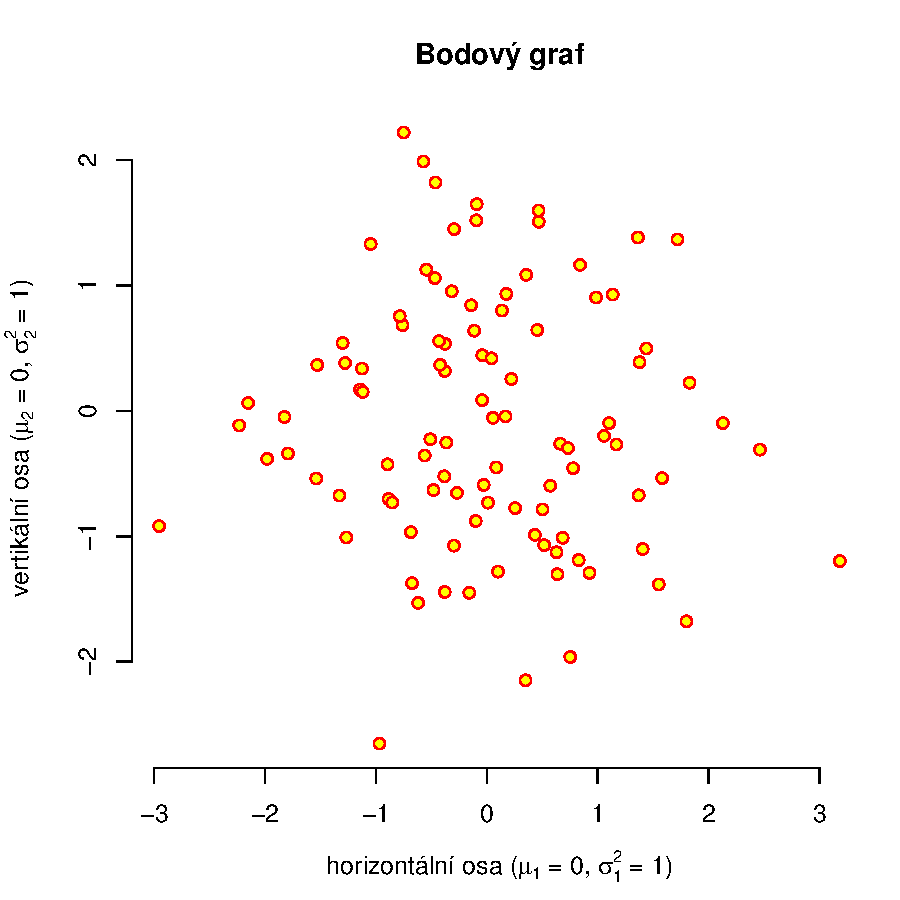
\includegraphics[width=.6\linewidth]{img/ukazka-obr01.pdf}
\caption{This caption is a friendly reminder to never insert figures ``in text,'' without a floating environment, unless explicitly needed for maintaining the text flow (e.g., the figure is small and developing with the text, like some of the centered equations, as in \cref{thm:y}). All figures \emph{must} be referenced by number from the text (so that the readers can find them when they read the text) and properly captioned (so that the readers can interpret the figure even if they look at it before reading the text --- reviewers love to do that).}
\label{fig:f}
\end{figure}

It is sometimes convenient (even recommended by some journals, including Cell) to name the results sub-sections so that they state what exactly has been achieved. Examples follow.

\section{SuperProgram is faster than OldAlgorithm}
\subsection{Scalability estimation}
\subsection{Precision of the results}
\section{Weird theorem is proven by induction}
\section{Amount of code reduced by CodeRedTool}
\subsection{Example}
\subsection{Performance on real codebases}
\section{\sloppy NeuroticHelper improves neural network learning}

\section{Graphics and figure quality}

No matter how great the text content of your thesis is, the pictures will always catch the attention first. This creates the very important first impression of the thesis contents and general quality. Crucially, that also decides whether the thesis is later read with joy, or carefully examined with suspicion.

Preparing your thesis in a way such that this first impression gets communicated smoothly and precisely helps both the reviewer and you: the reviewer will not have a hard time understanding what exactly you wanted to convey, and you will get a better grade.

Making the graphics `work for you' involves doing some extra work that is often unexpected. At the same time, you will need to fit into graphics quality constraints and guidelines that are rarely understood before you actually see a bad example. As a rule of thumb, you should allocate at least the same amount of time and effort for making the figures look good as you would for writing, editing and correcting the same page area of paragraph text.

\subsection{Visualize all important ideas}
The set of figures in your thesis should be comprehensive and complete. For all important ideas, constructions, complicated setups and results there should be a visualization that the reader can refer to in case the text does not paint the `mental image' sufficiently well. At the bare minimum, you should have at least 3 figures (roughly corresponding to the 3 chapters) that clearly and unambiguously show:
\begin{enumerate}
\item the context of the problem you are solving, optionally with e.g.~question marks and exclamation marks placed to highlight the problems and research questions
\item the overall architecture of your solution (usually as a diagram with arrows, such as in \cref{fig:schema}, ideally with tiny toy examples of the inputs and outputs of each box),
\item the advancement or the distinctive property of your solution, usually in a benchmark plot, or as a clear demonstration and comparison of your results.
\end{enumerate}

\subsection{Make the figures comprehensible}
The figures should be easily comprehensible. Surprisingly, that requires you to follow some common ``standards'' in figure design and processing. People are often used to a certain form of the visualizations, and (unless you have a very good reason) deviating from the standard is going to make the comprehension much more complicated. The common standards include the following:
\begin{itemize}
  \item caption everything correctly, place the caption at an expectable position
  \item systematically label the plots with `main' titles (usually in boldface, above the plot), plot axes, axis units and ticks, and legends
  \item lay out the diagrams systematically, ideally follow a structure of a bottom-up tree, a left-to-right pipeline, a top-down layered architecture, or a center-to-borders mindmap
  \item {use colors that convey the required information correctly \par\footnotesize Although many people carry some intuition for color use, achieving a really correct utilization of colors is often very hard without previous experience in color science and typesetting. Always remember that everyone perceives color hues differently, therefore the best distinction between the colors is done by varying lightness of the graphics elements (i.e., separating the data by dark vs.~light) rather than by using hues (i.e., forcing people to guess which one of salmon and olive colors means ``better''). Almost 10\% of the population have their vision impaired by some form of color vision deficiency, most frequently by deuteranomaly that prevents interpretation of even the most `obvious' hue differences, such as green vs.~red. Finally, printed colors look surprisingly different from the on-screen colors. You can prevent much of these problems by using standardized palettes and well-tested color gradients, such as the ones from ColorBrewer\footnote{\url{https://colorbrewer2.org}} and ViridisLite\footnote{\url{https://sjmgarnier.github.io/viridisLite/}}. Check if your pictures still look good if converted to greyscale, and use a color deficiency simulator to check how the colors are perceived with deuteranomaly.}
\end{itemize}

Avoid large areas of over-saturated and dark colors:
\begin{itemize}
  \item under no circumstances use dark backgrounds for any graphical elements, such as diagram boxes and tables --- use very light, slightly desaturated colors instead
  \item avoid using figures that contain lots of dark color (as a common example, heatmaps rendered with the `magma' color palette often look like huge black slabs that are visible even through the paper sheet, thus making a dark smudge on the neighboring page)
  \item increase the brightness of any photos to match the average brightness of the text around the figure
\end{itemize}

Remember to test your figures on other people --- usually, just asking `What do you think the figure should show?' can help you debug many mistakes in your graphics. If they think that the figure says something different than what you planned, then most likely it is your figure what is wrong, not the understanding of others.

Finally, there are many magnificent resources that help you arrange your graphics correctly. The two books by Tufte are arguably classics in the area. Additionally, you may find many interesting resources to help you with technical aspects of plotting, such as the \texttt{ggplot}-style `Fundamentals' book by, and a wonderful manual for the TikZ/PGF graphics system by that will help you draw high-quality diagrams (like the one in~\cref{fig:schema}).

\section{What is a discussion?}
After you present the results and show that your contributions work, it is important to \emph{interpret} them, showing what they mean in the wider context of the thesis topic, for the researchers who work in the area, and for the more general public, such as for the users.

Separate discussion sections are therefore common in life sciences where some ambiguity in result interpretation is common, and the carefully developed intuition about the wider context is sometimes the only thing that the authors have. Exact sciences and mathematicians do not need to use the discussion sections as often. Despite of that, it is nice to position your output into the previously existing environment, answering:
\begin{itemize}
\item What is the potential application of the result?
\item Does the result solve a problem that other people encountered?
\item Did the results point to any new (surprising) facts?
\item How (and why) is the approach you chose different from what the others have done previously?
\item Why is the result important for your future work (or work of anyone other)?
\item Can the results be used to replace (and improve) anything that is used currently?
\end{itemize}

If you do not know the answers, you may want to ask the supervisor. Also, do not worry if the discussion section is half-empty or completely pointless; you may remove it completely without much consequence. It is just a bachelor thesis, not a world-saving avenger thesis.

\chapwithtoc{Závěr}
V této práci jsme zkoumali vliv meteorologických podmínek na rozdíl teplot v blízkosti zemského povrchu v lesním porostu. K tomu jsme využili data z meteorologických stanic a ze $157$ čidel rozmístěných napříč národními parky Šumava a Bavorský les. Ke zpracování byla dostupná data za období od 12.10.2019 do 17.5.2021. Spočítali jsme 32 lineární smíšených modelů rozdělených do hlavních skupin podle toho, jestli závislá proměnná byla v absolutní hodnotě (modely s absolutní hodnotou), jestli jsme studovali maximální nebo minimální teploty, a nebo jestli zdroj teplot u země bylo čidlo ve výšce $\SI{0}{cm}$ nebo $\SI{15}{cm}$. Nulovou hypotézu jsme pomocí modelů vyvrátili a zjistili, že mezi rozdílem maximálních, resp. minimálních denních teplot na čidlech ve výšce $\SI{0}{cm}$, resp. $\SI{15}{cm}$ a $\SI{2}{m}$ a meteorologickými proměnnými ze staničních měření existuje vztah, neboli jejich koeficienty jsou pro většinu modelů nenulové. Tento vztah jsme zkoumali u řady prediktorů: výška sněhu, oblačnost, půdní vlhkost, množství srážek, rychlost větru a insolace.

Kromě statistického zpracování dat jsme také provedli interpretaci výsledků v kontextu rešerše dostupných znalostí z oblasti mikroklimatologie a mikrometeorologie. Ukázali jsme, že výška sněhu má kladný vliv na rozdíl teplot a nahrazení výšky sněhu za kategorickou proměnnou (žádný sníh, čidlo nad sněhem a čidlo pod sněhem) může výrazně zvýšit sílu prediktoru. Jako hlavní vliv výšky sněhu jsme určili to, že pod dostatečnou vrstvou sněhu se teplota pohybuje okolo $\SI{0}{\celsius}$. Prediktor oblačnosti má silný záporný vliv na rozdíl teplot především proto, že při větší oblačnosti dochází k menšímu ohřevu povrchu. Rychlost větru má záporný vliv na rozdíl teplot, protože dochází k silnějšímu promíchávání vzduchu. Insolace má slabý kladný vliv, protože souvisí s ohřevem povrchu. Množství srážek byl nejméně průkazný prediktor, který pro některé modely ukazoval pokles absolutního rozdílu teplot, který byl silnější pro čidla ve výšce $\SI{0}{cm}$. Půdní vlhkost byla silným prediktorem, který se ovšem výrazně lišil mezi modely s a bez absolutní hodnoty a mezi jednotlivými částmi roku. Možné důvody jsme uvedli v diskuzi. Hlavním důvodem pro nejistotu v interpretaci všech prediktorů byla relativní vzdálenost čidel od meteorologických stanic, které měřily meteorologické podmínky. Nebylo zde tedy v některých případech možné udělat hlubší analýzu problematiky kvůli kvalitě dat.

Dále jsme navrhli způsob, jak možnosti studia mikroklimatu vylepšit. Kvalita analýzy by byla výrazně vylepšena měřením meteorologických podmínek i v lesním porostu, ale také zpracováním delšího časového období z následujících let. Také jsme při zpracování dat nebrali v potaz rozdílný vliv topografie a vegetace na každé čidlo a kvůli tomu modely nemohly vysvětlit více variability rozdílu teplot. Některé prediktory bychom mohli v hlubší analýze upravit nebo nahradit jinými. Ze statistického hlediska by největším zlepšením zřejmě bylo vytvořit složitější prostoročasový model. Výsledky práce otevírají možnosti dalšímu výzkumu, který by mohl vést například k interpolaci chybějících mikroklimatických dat, a pomáhají nám porozumět interakci mezi teplotami v lesním porostu a ostatními meteorologickými podmínkami.


\ifEN
\chapwithtoc{Bibliography}
\else
\chapwithtoc{Seznam použité literatury}
\fi

\printbibliography[heading=none]


%\appendix
%\chapter{Using CoolThesisSoftware}

Use this appendix to tell the readers (specifically the reviewer) how to use your software. A very reduced example follows; expand as necessary. Description of the program usage (e.g., how to process some example data) should be included as well.

To compile and run the software, you need dependencies XXX and YYY and a C compiler. On Debian-based Linux systems (such as Ubuntu), you may install these dependencies with APT:
\begin{Verbatim}
apt-get install \
  libsuperdependency-dev \
  libanotherdependency-dev \
  build-essential
\end{Verbatim}

To unpack and compile the software, proceed as follows:
\begin{Verbatim}
unzip coolsoft.zip
cd coolsoft
./configure
make
\end{Verbatim}

The program can be used as a C++ library, the simplest use is demonstrated in \cref{lst:ex}. A demonstration program that processes demonstration data is available in directory \verb|demo/|, you can run the program on a demonstration dataset as follows:
\begin{Verbatim}
cd demo/
./bin/cool_process_data data/demo1
\end{Verbatim}

After the program starts, control the data avenger with standard \verb-WSAD- controls.

\begin{listing}
\begin{lstlisting}
#include <CoolSoft.h>
#include <iostream>

int main() {
	int i;
	if(i = cool::ProcessAllData()) // returns 0 on error
		std::cout << i << std::endl;
	else
		std::cerr << "error!" << std::endl;
	return 0;
}
\end{lstlisting}
\caption{Example program.}
\label{lst:ex}
\end{listing}


% if your attachments are complicated, describe them in a separate appendix
%\include{attachments}

\openright
\end{document}
